\documentclass{amsart}
%%%%%%%%%%%%%%%%%%%%%%%%%%%%%%%%%%%
\usepackage{amssymb}
\usepackage{amsfonts}
\usepackage{graphicx}
\usepackage{subfig}
\usepackage{mathrsfs}
\usepackage{enumerate}
\usepackage[hypertexnames=false]{hyperref}
\hypersetup{colorlinks=true,linkcolor=blue,pdfborder = {0 0 0.1}}

\renewcommand{\Re}{\mathrm{Re}}
\setcounter{MaxMatrixCols}{10}

\newtheorem{theorem}{Theorem}%[section]
\newtheorem{lemma}[theorem]{Lemma}
\theoremstyle{definition}
\newtheorem{definition}[theorem]{Definition}
\newtheorem{example}[theorem]{Example}
\newtheorem{counterexample}[theorem]{Counterexample}
\newtheorem{xca}[theorem]{Exercise}
\theoremstyle{remark}
\newtheorem{remark}[theorem]{Remark}
\numberwithin{equation}{section}
\theoremstyle{plain}
\newtheorem{acknowledgement}{Acknowledgement}
\newtheorem{algorithm}{Algorithm}
\newtheorem{axiom}{Axiom}
\newtheorem{case}{Case}
\newtheorem{claim}{Claim}
\newtheorem{conclusion}{Conclusion}
\newtheorem{condition}{Condition}
\newtheorem{conjecture}[theorem]{Conjecture}
\newtheorem{falsehood}[theorem]{Falsehood}
\newtheorem{question}[theorem]{Question}
\newtheorem{corollary}[theorem]{Corollary}
\newtheorem{criterion}{Criterion}
\newtheorem{exercise}{Exercise}
\newtheorem{notation}{Notation}
\newtheorem{proposition}[theorem]{Proposition}
\newtheorem{summary}{Summary}
\theoremstyle{definition}
\newtheorem{solution}{Solution}
\newtheorem{problem}{Problem}

\renewcommand{\Re}{\mathscr{R}} 
\setcounter{section}{-1}

\begin{document}
\title{Solutions to Rainville's \textquotedblleft Special Functions" (1960)}
\author{solutions by Sylvester J. Pagano and Leon Hall; ed. Tom Cuchta}

\maketitle 

%\addtocontents{toc}{\protect\hypertarget{toc}{}}
\tableofcontents \label{toc}

\date{\today}
\newpage
\section{Preface}
Earl D. Rainville began giving lectures on Special Functions at the University of Michigan in 1946.  The course was well received, and his notes became the basis for his book, Special Functions, published in 1960.  Also in 1946, Sylvester J. Pagano received his B.S. degree in Electrical Engineering at the Missouri School of Mines and Metallurgy (MSM).  That fall, Pagano was appointed Instructor in Mathematics at MSM.  In 1950, Pagano, now Assistant Professor, spent the summer at Michigan, where he and Rainville presumably met.  In the summers of 1962, 1963, and 1964, Pagano was again at Michigan, this time as a National Science Foundation Science Faculty Fellow.  Rainville passed away in 1966, the same year Pagano was promoted to Professor at the University of Missouri--–Rolla (UMR, MSM under its new name).  In the spring of 1966, I was a sophomore at UMR and was taking Elementary Differential Equations; the textbook was the third edition or so of Rainville's Elementary Differential Equations.  This would be a better story if Pagano had been the instructor in that class, but he wasn't.  I did have a class from Pagano later, when I was a beginning graduate student; it was Operational Calculus, and we used the Operational Mathematics book by R.V. Churchill.  Churchill was Rainville's Ph.D. advisor (Michigan 1939), but I knew nothing of any of these connections at the time.  Pagano was a member of both my M.S. and Ph.D. committees at UMR.

\begin{figure}[h]
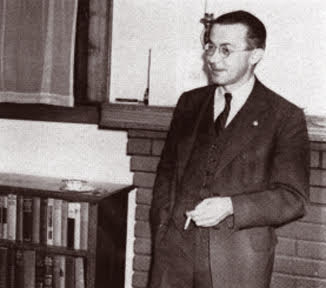
\includegraphics[scale=0.9]{images/rainville.jpg}
\caption{Photograph of Earl D. Rainville from the \href{http://um2017.org/faculty-history/faculty/earl-david-rainville}{University of Michigan}.}
\end{figure}
\newpage Pagano retired in 1986, a year after I had returned to Rolla as a faculty member.  Somehow, in the process of him cleaning out his office, I got his collections of worked problems from Rainville's Special Functions, Rainville's Intermediate Differential Equations, and Churchill's Operational Mathematics.  The way I remember it is that I knew these problem solutions existed, and when Pagano retired, I asked him if I could have them, a request to which he graciously agreed.  As to how I knew he even had this material, I don't remember for sure.  These problem solutions (hand--written) almost certainly go back to the three summers Pagano spent at Michigan in the 1960s, and some might even date back to his earlier 1950 visit; Pagano continued to work on them as he taught the courses himself in the 1960s--1980s.  

\begin{figure}
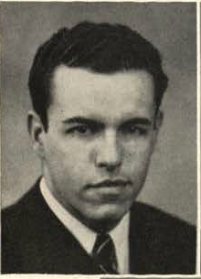
\includegraphics[scale=0.7]{images/pagano2.png}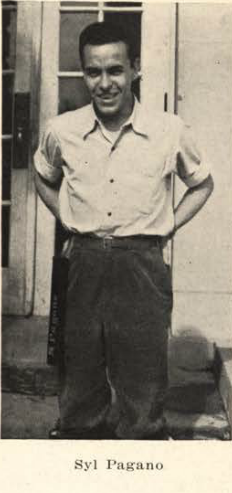
\includegraphics[scale=0.4]{images/pagano1.png}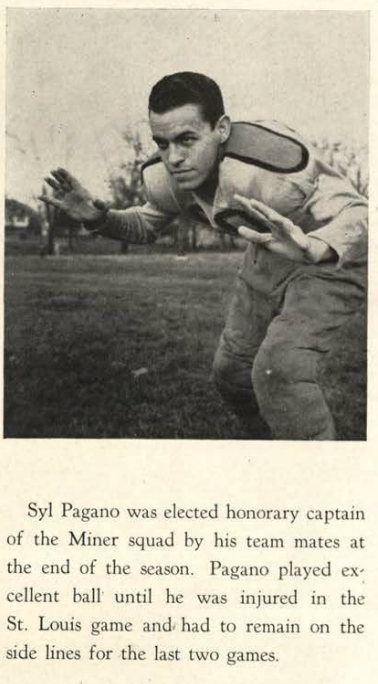
\includegraphics[scale=0.3]{images/pagano3.png}
\caption{These photographs are of Sylvester J. Pagano as a college senior in 1946.}
\end{figure}
Beginning in the mid--1990s I began to teach both Operational Calculus and Special Functions from time to time at UMR.  For Operational Calculus, I used Churchill's book, and Pagano's problem solutions were quite useful.  I developed my own notes for Special Functions because it was a summer course designed so our graduate students who taught in the summer would have something to take, and some of these students had not yet studied complex variables.  The last time I offered Special Functions was the summer of 2012, and I was able to talk Tom Cuchta, one of the students in that class, into working on transcribing Pagano's problem solutions from Rainville's Special Functions into electronic form using \LaTeX .  To my surprise and delight, Cuchta finished the job by the end of 2012!  We learned, however, that Pagano had not provided solutions to all the problems – he wrote up solutions to 196 out of 231 problems in the book.  That's 85$\%$, so is pretty good, but I decided I would work on finishing the job, and Cuchta agreed to keep adding to the \TeX file as more problems were completed.  As of now (April 2015), there are less than 10 problems left to finish.  The end is in sight.

Sylvester Pagano was a good example of a type of mathematics professor that seems to be disappearing these days.  He didn't publish any papers, but he was an outstanding teacher and he kept building his knowledge of mathematics throughout his career.  When I talk with alumni from our department, and often with engineering graduates from other departments, the person they most frequently ask about is Professor Pagano; they fondly remember him as one of the good ones from their student days.  These alums are right---he was one of the good ones, and he should be remembered.  These problem solutions are mostly his, and the rest were inspired by him.  There is a lot of interesting mathematics here.  I hope you enjoy it.\vspace{10pt}\\
Leon M. Hall \\
Professor Emeritus, Mathematics\\
Missouri S$\&$T
%%%%
%%
%%
%%%%
%%%% CHAPTER 1
%%%% CHAPTER 1
%%%%
%%
%%
%%%%

\section{Chapter 1 Solutions}
\begin{center}\hyperref[toc]{\^{}\^{}}\end{center}
\begin{center}\begin{tabular}{lllllllllllllllllllllllll}
\hyperref[problem1chapter1]{P1} & \hyperref[problem2chapter1]{P2} & \hyperref[problem3chapter1]{P3} & \hyperref[problem4chapter1]{P4} & \hyperref[problem5chapter1]{P5} & \hyperref[problem6chapter1]{P6} & \hyperref[problem7chapter1]{P7} & \hyperref[problem8chapter1]{P8} & \hyperref[problem9chapter1]{P9} & \hyperref[problem10chapter1]{P10} & \hyperref[problem11chapter1]{P11} 
\end{tabular}\end{center}
\begin{problem}\label{problem1chapter1}
Show that the following product converges and find its value: 
$$\displaystyle\prod_{n=1}^{\infty} \left[ 1 + \dfrac{6}{(n+1)(2n+9)} \right].$$
\end{problem}
\begin{solution}(Solution by Leon Hall)
By Theorem 3, page 3, this product converges absolutely because $\displaystyle\sum_{n=1}^{\infty} \dfrac{6}{(n+1)(2n+9)}$ converges absolutely.
$$\begin{array}{ll}
1 + \dfrac{6}{(n+1)(2n+9)} &= \dfrac{(n+1)(2n+9)+6}{(n+1)(2n+9)} \\
&= \dfrac{2n^2+11n+15}{(n+1)(2n+9)} \\
&= \dfrac{(2n+5)(n+3)}{(n+1)(2n+9)}.
\end{array}$$
So, if 
$$\begin{array}{ll}
P_n &= \displaystyle\prod_{k=1}^n \left[ 1 + \dfrac{6}{(k+1)(2k+9)} \right] \\
&= \displaystyle\prod_{k=1}^n \dfrac{(2k+5)(k+3)}{(k+1)(2k+9)} \\
&= \dfrac{[7 \cdot 9 \cdot  \cdot  \cdot (2n+5)][4 \cdot 5 \cdot  \cdot  \cdot (n+3)]}{[2 \cdot 3 \cdot  \cdot  \cdot (n+1)][11 \cdot 13 \cdot  \cdot  \cdot  (2n+9)]} \\
&= \dfrac{[7 \cdot 9][(n+2) (n+3)]}{[2 \cdot 3][(2n+7) (2n+9)]} \\
&= \dfrac{21}{2} \dfrac{(n+2)(n+3)}{(2n+7)(2n+9)}
\end{array}$$
then
$$\displaystyle\lim_{n \rightarrow \infty} P_n = \displaystyle\lim_{n \rightarrow \infty} \dfrac{21}{2} \dfrac{n^2 + 5n+6}{4n^2+32n+63} = \dfrac{21}{8}.$$
Note: The use of Theorem 3 is not needed because finding the value of the infinite product is sufficient itself to show convergence.
\end{solution}
%%%%
%%
%%
%%%%
\newpage
\begin{problem}\label{problem2chapter1}
Show that $\displaystyle\prod_{n=2}^{\infty} \left( 1 - \dfrac{1}{n^2} \right) = \dfrac{1}{2}$.
\end{problem}
\begin{solution}(Solution by Leon Hall)
First compute
$$1 - \dfrac{1}{n^2} = \dfrac{n^2-1}{n^2} = \dfrac{(n+1)(n-1)}{n^2}.$$
Let
$$\begin{array}{ll}
P_n &= \displaystyle\prod_{k=2}^n \left( 1 - \dfrac{1}{k^2} \right) \\
&= \displaystyle\prod_{k=2}^n \dfrac{(k+1)(k-1)}{k^2} \\
&= \dfrac{[3 \cdot 4 \cdot  \cdot  \cdot (n+1)][1 \cdot 2 \cdot 3 \cdot  \cdot  \cdot (n-1)]}{(2 \cdot 3 \cdot 4 \cdot  \cdot  \cdot n)^2} \\
&= \dfrac{(n+1)}{2n}. \\
\end{array}$$
Then,
$$\begin{array}{ll}
\displaystyle\lim_{n \rightarrow \infty} P_n &= \displaystyle\lim_{n \rightarrow \infty} \dfrac{n+1}{2n} \\ 
&= \dfrac{1}{2} \\
&= \displaystyle\prod_{n=2}^{\infty} \left( 1 - \dfrac{1}{n^2} \right).
\end{array}$$
\end{solution}
%%%%
%%
%%
%%%%
\begin{problem}\label{problem3chapter1}
Show that $\displaystyle\prod_{n=2}^{\infty} \left( 1 - \dfrac{1}{n} \right)$ diverges to $0$.
\end{problem}
\begin{solution}(Solution by Leon Hall)
$$P_n = \displaystyle\prod_{k=2}^n \left( \dfrac{k-1}{k} \right) = \dfrac{1 \cdot 2 \cdot 3 \cdot  \cdot  \cdot (k-1)}{2 \cdot 3 \cdot 4  \cdot  \cdot  \cdot  n} = \dfrac{1}{n}$$
Since
$$\displaystyle\lim_{n \rightarrow \infty} P_n = \displaystyle\lim_{n \rightarrow \infty} \dfrac{1}{n} = 0$$
the product diverges to $0$. [The product does not converge to $0$ because none of the terms in the product are $0$.]
\end{solution}
%%%%
%%
%%
%%%%
\begin{problem}\label{problem4chapter1}
Investigate the product $\displaystyle\prod_{n=0}^{\infty} (1 + z^{2^n})$ in $|z| < 1$.
\end{problem}
\begin{solution}(Solution by Leon Hall)
Let $P_n = \displaystyle\prod_{k=0}^n (1 + z^{2^k})$. Then
$$P_0 = 1+z,$$
$$P_1 = (1+z)(1+z^2)$$
$$P_2 = (1+z)(1+z^2)(1+z^4) = (1+z)(1+z^2+z^4+z^6).$$
Assume $P_n = (1+z) \displaystyle\sum_{k=0}^{2(2^n-1)} (z^2)^k = \displaystyle\sum_{k=0}^{2^{n+1}-2} (z^2)^k.$ Then
$$\begin{array}{ll}
P_{n+1} &= P_n(1+z^{2^{n+1}} ) \\
&= P_n + z^{2^{n+1}}P_n \\
&= (1+z) \left[ 1+ z^2 + \cdot \cdot \cdot + z^{2^{n+1}-2}+z^{2^{n+1}} + z^{2^{n+1}+2} + \cdot \cdot \cdot + z^{2^{n+2}-2} \right] \\
&= (1+z) \displaystyle\sum_{k=0}^{2^{n+2}-2} (z^2)^k
\end{array}$$
So we have shown by induction that
$$P_n = (1+z) \displaystyle\sum_{k=0}^{2^{n+1}-2} z^{2k},$$
which is a geometric series converging to $(z+1) \dfrac{1}{1-z^2}$, for $|z|<1$. 
$$|1+z^{2^n}| \leq 1 + |z|^{2^n}$$
and same process works. Thus, $\displaystyle\prod_{n=0}^{\infty} (1+z^{2^n})$ converges absolutely to $\dfrac{1}{1-z}$.
\end{solution}
%%%%
%%
%%
%%%%
\begin{problem}\label{problem5chapter1}
Show that $\displaystyle\prod_{n=1}^{\infty} \exp \left( \dfrac{1}{n} \right)$ diverges.
\end{problem}
\begin{solution}(Solution by Leon Hall)
Let $P_n = \displaystyle\prod_{k=1}^n \exp \left( \dfrac{1}{n} \right)$ and let 
$$S_n = \log P_n = \displaystyle\sum_{k=1}^n \dfrac{1}{k}.$$
$S_n$ is the $n$th partial sum of the harmonic series, which diverges. As in the proof of Theorem 2, page 3, $P_n = \exp S_n$ and
$$\displaystyle\lim_{n \rightarrow \infty} P_n = \displaystyle\lim_{n \rightarrow \infty} \exp S_n = \exp \displaystyle\lim_{n \rightarrow \infty} S_n.$$
Thus, because $\{S_n\}$ diverges, so does $\{P_n \}$.
\end{solution}
%%%%
%%
%%
%%%%
%%%%
%%
%%
%%%%
\begin{problem}\label{problem6chapter1}
Show that $\displaystyle\prod_{n=1}^{\infty} \exp \left( - \dfrac{1}{n} \right)$ diverges to $0$.
\end{problem}
\begin{solution}(Solution by Leon Hall)
Let 
$$\log P_n = S_n = \displaystyle\sum_{k=1}^n \left( - \dfrac{1}{k} \right) = - \displaystyle\sum_{k=1}^n \dfrac{1}{k}$$
as in Problem 5. Then
$$P_n = \exp S_n = \exp \left( -\displaystyle\sum_{k=1}^n \dfrac{1}{k} \right) = \dfrac{1}{\exp \left( \displaystyle\sum_{k=1}^n \dfrac{1}{k} \right)}.$$
Because $\displaystyle\sum_{k=1}^{\infty} \dfrac{1}{k}$ diverges to $\infty$ we have
$$\displaystyle\lim_{n \rightarrow \infty} P_n = 0$$
and so
$$\displaystyle\prod_{n=1}^{\infty} \exp \left( - \dfrac{1}{n} \right)$$
diverges to $0$.
\end{solution}
%%%%
%%
%%
%%%%
%%%%
%%
%%
%%%%
\begin{problem}\label{problem7chapter1}
Test $\displaystyle\prod_{n=1}^{\infty} \left( 1 - \dfrac{z^2}{n^2} \right).$
\end{problem}
\begin{solution}(Solution by Leon Hall)
The product diverges to $0$ for any $z$ such that $z = \pm m$, $m$ a positive integer. For all $z$ such that $1 - \dfrac{z^2}{n^2} \neq 0$, we have by Theorem 3, page 3, that $\displaystyle\prod_{n=1}^{\infty} \left( 1 - \dfrac{z^2}{n^2} \right)$ is absolutely convergent because $\displaystyle\sum_{n=1}^{\infty} \left( - \dfrac{z^2}{n^2} \right)$ is absolutely convergent. In fact,
$$\displaystyle\sum_{n=1}^{\infty} \left( - \dfrac{z^2}{n^2} \right) = -\dfrac{z^2 \pi^2}{6}.$$
\end{solution}
%%%%
%%
%%
%%%%
%%%%
%%
%%
%%%%
\begin{problem}\label{problem8chapter1}
Show that $\displaystyle\prod_{n=1}^{\infty} \left[ 1 + \dfrac{(-1)^{n+1}}{n} \right]$ converges to unity.
\end{problem}
\begin{solution}(Solution by Leon Hall)
Let $P_n = \displaystyle\prod_{k=1}^n \left[ 1 + \dfrac{(-1)^{k+1}}{k} \right]$.

Case 1: $n$ is even. Then
$$P_n = \left( \dfrac{1+1}{1} \right) \left( \dfrac{2-1}{2} \right) \left( \dfrac{3+1}{3} \right) \left( \dfrac{4-1}{4} \right) \cdot \cdot \cdot  \left( \dfrac{n}{n-1}  \right) \left( \dfrac{n-1}{n} \right)$$ 
Rearranging, we get $P_n = \dfrac{n!}{n!} = 1$ for even $n$.

Case 2: $n$ is odd. Then
$$P_n = \left( \dfrac{1+1}{1} \right) \left( \dfrac{2-1}{2} \right) \left( \dfrac{3+1}{3} \right) \left( \dfrac{4-1}{4} \right)  \cdot \cdot \cdot \left( \dfrac{n-1}{n-2} \right) \left( \dfrac{n-2}{n-1} \right) \left( \dfrac{n+1}{n} \right)  = \dfrac{n+1}{n}.$$

In both cases $\displaystyle\lim_{n \rightarrow \infty} P_n = 1$.
\end{solution}
%%%%
%%
%%
%%%%
%%%%
%%
%%
%%%%
\begin{problem}\label{problem9chapter1}
Test for convergence: $\displaystyle\prod_{n=2}^{\infty} \left( 1 - \dfrac{1}{n^p} \right)$ for real $p \neq 0$.
\end{problem}
\begin{solution}(Solution by Leon Hall)
For $p>1$ the series of positive numbers $\displaystyle\sum_{n=2}^{\infty} \dfrac{1}{n^p}$ is known to be convergent (e.g., by the Integral Test). Thus, $\displaystyle\prod_{n=2}^{\infty} \left( 1 - \dfrac{1}{n^p} \right)$ is absolutely convergent by Theorem 3.

For $0 < p \leq 1$, $1 - \dfrac{1}{n^p} > 0$ and so convergence and absolute convergence are the same. Because the series $\displaystyle\sum_{n=2}^{\infty} \dfrac{1}{n^p}$ diverges for $0 < p \leq 1$, our product diverges by Theorem 3.

For $p < 0$, let $p = -q$ where $q > 0$. Then
$$1 - \dfrac{1}{n^p} = 1 - n^q = 1 + (-n^q).$$
But $\displaystyle\lim_{n \rightarrow \infty} (-n^q) \neq 0$, so in this case our product diverges by Theorem~1. 

Summary: $\displaystyle\prod_{n=2}^{\infty} \left( 1 - \dfrac{1}{n^p} \right)$ diverges when $p \leq 1$ (an $p \neq 0$), and converges when $p > 1$.
\end{solution}
%%%%
%%
%%
%%%%
%%%%
%%
%%
%%%%
\begin{problem}\label{problem10chapter1}
Show that $\displaystyle\prod_{n=1}^{\infty} \dfrac{\sin ( \frac{z}{n})}{\frac{z}{n}}$ is absolutely convergent for all finite $z$ with the usual convention at $z=0$.
\end{problem}
\begin{solution}(Solution by Leon Hall)
Let
$$\dfrac{\sin(\frac{z}{n})}{\frac{z}{n}} = 1 + a_n(z).$$
Then
$$\begin{array}{ll}
a_n(z) &= \dfrac{\sin(\frac{z}{n})}{\frac{z}{n}} - 1 \\
&= -\dfrac{1}{3!} \dfrac{z^2}{n^2} + \dfrac{1}{5!} \dfrac{z^4}{n^4} - \dfrac{1}{7!} \dfrac{z^6}{n^6} + \ldots \\
&= \dfrac{1}{n^2} \left[ -\dfrac{z^2}{6} + \mathcal{O} \left( \dfrac{1}{n^2} \right) \right].
\end{array}$$
Thus, there exists a constant $M$ such that
$$|a_n(z)| < \dfrac{M}{n^2},$$
and because $\displaystyle\sum_{n=1}^{\infty} \dfrac{M}{n^2}$ converges, the product
$$\displaystyle\prod_{n=1}^{\infty} (1+a_n(z)) = \dfrac{\sin(\frac{z}{n})}{\frac{z}{n}}$$
converges absolutely and uniformly for all finite $z$ by Theorems 3 and 4. 

If $z=0$ the product is, with the usual convention,
$$\displaystyle\prod_{n=1}^{\infty} 1 = 1.$$
\end{solution}
%%%%
%%
%%
%%%%
\begin{problem}\label{problem11chapter1}
Show that if $c$ is not a negative integer,
$$\displaystyle\prod_{n=1}^{\infty} \left[ \left( 1 - \dfrac{z}{c+n} \right) \exp \left( \dfrac{z}{n} \right) \right]$$
is absolutely convergent for all finite $z$.
\end{problem}
\begin{solution}
Let
\begin{eqnarray*}
\lefteqn{1+a_n(z)} \\
& &= \left( 1 - \dfrac{z}{c+n} \right) \exp \left( \dfrac{z}{n} \right) \\
& &= \left( 1 + \dfrac{z}{n} + \dfrac{1}{2!} \dfrac{z^2}{n^2} + \dfrac{1}{3!} \dfrac{z^3}{n^3} + \ldots \right) - \dfrac{1}{c+n} \left( z + \dfrac{z^2}{n} + \dfrac{1}{2!} \dfrac{z^3}{n^2} + \dfrac{1}{3!} \dfrac{z^4}{n^3} + \ldots \right) \\
& &= 1 + \left( \dfrac{1}{n} - \dfrac{1}{c+n} \right)z + \left( \dfrac{1}{2!n^2} - \dfrac{1}{n(c+n)} \right) z^2 \\
& & \phantom{=}+ \left( \dfrac{1}{3!n^3} - \dfrac{1}{2! n^2(c+n)} \right) z^3 + \ldots \\
& &= 1 + \dfrac{c}{n(c+n)}z + \dfrac{c-n}{2n^2(c+n)}z^2 + \displaystyle\sum_{k=3}^{\infty} \dfrac{c - (k-1)n}{k! n^k (c+n)} z^k \\
& &= 1 + \dfrac{c}{n(c+n)}z - \dfrac{1}{2n(c+n)} z^2 + \mathcal{O} \left( \dfrac{1}{n^2} \right).
\end{eqnarray*}
Thus, for $c$ not a negative integer and for any finite $z$, there is a constant $M$ such that $|a_n(z)| \leq \dfrac{M}{n^2}$ and so by Theorems 3 and 4 the product converges absolutely and uniformly.
\end{solution}

%%%%
%%
%%
%%%%
%%%% CHAPTER 2
%%%% CHAPTER 2
%%%%
%%
%%
%%%%
\section{Chapter 2 Solutions}
\begin{center}\hyperref[toc]{\^{}\^{}}\end{center}
\begin{center}\begin{tabular}{lllllllllllllllllllllllll}
\hyperref[problem1chapter2]{P1} & \hyperref[problem2chapter2]{P2} & \hyperref[problem3chapter2]{P3} & \hyperref[problem4chapter2]{P4} & \hyperref[problem5chapter2]{P5} & \hyperref[problem6chapter2]{P6} & \hyperref[problem7chapter2]{P7} & \hyperref[problem8chapter2]{P8} & \hyperref[problem9chapter2]{P9} & \hyperref[problem10chapter2]{P10} & \hyperref[problem11chapter2]{P11} & \hyperref[problem12chapter2]{P12} & \hyperref[problem13chapter2]{P13} & \hyperref[problem14chapter2]{P14} & \hyperref[problem15chapter2]{P15} & 
\end{tabular}\end{center}
\setcounter{problem}{0}
\setcounter{solution}{0}
\begin{problem}\label{problem1chapter2} %Problem 1
Start with 
$$(\dagger) \dfrac{\Gamma'(z)}{\Gamma(z)} = -\gamma - \dfrac{1}{z} - \displaystyle\sum_{n=1}^{\infty} \left( \dfrac{1}{z+n} - \dfrac{1}{n} \right),$$
prove that
$$\dfrac{2 \Gamma'(2z)}{\Gamma(2z)} - \dfrac{\Gamma'(z)}{\Gamma(z)} - \dfrac{\Gamma'(z+\frac{1}{2})}{\Gamma(z+\frac{1}{2})} = 2 \log 2,$$
and thus derive Legendre's duplication formula, page 24.
\end{problem}
\begin{solution}
Applying $(\dagger)$ three times and simplifying yields
\begin{eqnarray*}
\lefteqn{\dfrac{2 \Gamma'(2z)}{\Gamma(2z)} - \dfrac{\Gamma'(z)}{\Gamma(z)} - \dfrac{\Gamma'(z+\frac{1}{2})}{\Gamma(z+\frac{1}{2})}} \\
& &= -2 \gamma - \dfrac{2}{2z} + \gamma + \dfrac{1}{z} + \gamma + \dfrac{1}{z+\frac{1}{2}} - \displaystyle\sum_{n=1}^{\infty} \left( \dfrac{2}{2z+n} - \dfrac{2}{n} \right) + \displaystyle\sum_{n=1}^{\infty} \left( \dfrac{1}{z+n} - \dfrac{1}{n} \right) \\
& & \phantom{=}+ \displaystyle\sum_{n=1}^{\infty} \left( \dfrac{1}{z+\frac{1}{2}+n} - \dfrac{1}{n} \right) \\
& &= \dfrac{2}{2z+1} - \displaystyle\lim_{n \rightarrow \infty} \displaystyle\sum_{k=1}^{2n} \left( \dfrac{2}{2z+k} - \dfrac{2}{k} \right) + \displaystyle\lim_{n \rightarrow \infty} \displaystyle\sum_{k=1}^n \left( \dfrac{1}{z+k} - \dfrac{1}{k} \right) \\
& & \phantom{=}+ \displaystyle\lim_{n \rightarrow \infty} \displaystyle\sum_{k=1}^n \left( \dfrac{2}{2z+1+2k} - \dfrac{1}{k} \right) \\
& &= \dfrac{2}{2z+1} + \displaystyle\lim_{n \rightarrow \infty} \left[ \displaystyle\sum_{k=1}^{2n} \dfrac{-2}{2z+k} + 2 H_{2n} + \displaystyle\sum_{k=1}^n \dfrac{2}{2z+2k} - H_n \right. \\
& & \phantom{=} \left. + \displaystyle\sum_{k=1}^n \dfrac{2}{2z+2k+1} - H_n \right] \\
& &= \dfrac{2}{2z+1} + \displaystyle\lim_{n \rightarrow \infty} \left[ \displaystyle\sum_{k=1}^{2n} \dfrac{-2}{2z+k} + \displaystyle\sum_{k=2}^{2n+1} \dfrac{2}{2z+k} + 2 H_{2n} - 2 H_n \right] \\
& &= \dfrac{2}{2z+1} + \dfrac{-2}{2z+1} + \displaystyle\lim_{n \rightarrow \infty} \dfrac{2}{2z+2n+1} + \displaystyle\lim_{n \rightarrow \infty} (2 H_{2n} - 2 H_n) \\
& &= 0 + 0 + 2 \displaystyle\lim_{n \rightarrow \infty} \left[ (H_{2n}- \log 2n) - (H_n - \log n) + \log 2n - \log n \right] \\
& &= 2 [ \gamma - \gamma + \log 2 ] \\
& &= 2 \log 2. \qed
\end{eqnarray*}
\end{solution}
%%%%
%%
%%
%%%%
\begin{problem}\label{problem2chapter2}
Show that $\Gamma' \left(\dfrac{1}{2} \right) = -(\gamma + 2 \log 2) \sqrt{\pi}$.
\end{problem}
\begin{solution}
By Problem $\ref{problem1chapter2}$, we know that
$$\dfrac{2 \Gamma'(2z)}{\Gamma(2z)} - \dfrac{\Gamma'(z)}{\Gamma(z)} - \dfrac{\Gamma'(z+\frac{1}{2})}{\Gamma(z+\frac{1}{2})} = 2 \log 2.$$
Now let $z=\dfrac{1}{2}$ to get
$$2 \dfrac{\Gamma'(1)}{\Gamma(1)} - \dfrac{\Gamma' \left(\frac{1}{2} \right)}{\Gamma \left(\frac{1}{2} \right)} - \frac{\Gamma'(1)}{\Gamma(1)} = 2 \log 2,$$
and so, algebra yields
$$\dfrac{\Gamma'(\frac{1}{2})}{\Gamma(\frac{1}{2})} =\dfrac{\Gamma'(1)}{\Gamma(1)} - 2 \log 2.$$
But $\Gamma(1)=1, \Gamma'(1)=-\gamma, \Gamma(\frac{1}{2}) = \sqrt{\pi}$, hence
$$\dfrac{\Gamma'(\frac{1}{2})}{\sqrt{\pi}} = - \dfrac{\gamma}{1} - 2 \log 2,$$
and by rearrangement,
$$\Gamma'\left(\frac{1}{2} \right) = -(\gamma + 2 \log 2) \sqrt{\pi}. \qed$$
\end{solution}
%%%%
%%
%%
%%%%
\begin{problem}\label{problem3chapter2}
Use Euler's integral form $\Gamma(z) = \displaystyle\int_0^{\infty} e^{-t} t^{z-1} \mathrm{d}t$ to show that 
$$\Gamma(z+1) = z \Gamma(z).$$
\end{problem}
\begin{solution}
From $\Gamma(z) = \displaystyle\int_0^{\infty} e^{-t} t^{z-1} \mathrm{d}t$, for $\mathrm{Re}(z) > 0$, integration by parts yields
$$\begin{array}{ll|ll}
u = t^z & \mathrm{d}v = e^{-t} \mathrm{d}t  & \Gamma(z+1) &= \displaystyle\int_0^{\infty} e^{-t}t^z \mathrm{d}t \\
\mathrm{d}u = zt^{z-1} & v=-e^{-t} & &= \left[-t^z e^{-t} \right]_0^{\infty} + z \displaystyle\int_0^{\infty} e^{-t} t^{z-1} \mathrm{d}t \\
& & &= 0 + z \Gamma(z),
\end{array}$$
where $\displaystyle\lim_{t \rightarrow \infty} -t^z e^{-t}$ converges for $\Re(z) > 0 \qed$.
\end{solution}
%%%%
%%
%%
%%%%
\begin{problem}\label{problem4chapter2}
Show that $\Gamma(z) = \displaystyle\lim_{n \rightarrow \infty} n^z B(z,n)$.
\end{problem}
\begin{solution}
From page 28 (1), we know
$$\Gamma(z) = \displaystyle\lim_{n \rightarrow \infty} \dfrac{(n-1)! n^z}{
(z)_n},$$
but
$$B(z,n) = \dfrac{\Gamma(z)\Gamma(n)}{\Gamma(z+n)} = \dfrac{\Gamma(z)(n-1)!}{(z)_n \Gamma(z)} = \dfrac{(n-1)!}{(z)_n}.$$
Hence 
$$\Gamma(z) = \displaystyle\lim_{n \rightarrow \infty} n^z B(z,n). \qed$$
\end{solution}
%%%%
%%
%%
%%%%
\begin{problem}\label{problem5chapter2}
Derive the following properties of the beta function: 
\begin{enumerate}[(a)]
\item $pB(p,q+1) = qB(p+1,q)$;
\item $B(p,q) = B(p+1,q) + B(p,q+1)$;
\item $(p+q)B(p,q+1) = qB(p,q)$;
\item $B(p,q)B(p+q,r) = B(q,r)B(q+r,p)$.
\end{enumerate}
\end{problem}
\begin{solution}
\begin{enumerate}[(a)]
\item We know $B(p,q) = \dfrac{\Gamma(p)\Gamma(q)}{\Gamma(p+q)}$, so
$$pB(p,q+1) = \dfrac{p \Gamma(p)\Gamma(q+1)}{\Gamma(p+q+1)} = \dfrac{\Gamma(p+1) q \Gamma(q)}{\Gamma(p+1+q)} = qB(p+1,q).$$
(note: $p \rightarrow q$ and $q \rightarrow p$ -- is this the symmetric property?)
\item
$$\begin{array}{ll}
B(p,q) &= \dfrac{\Gamma(p)\Gamma(q)}{\Gamma(p+q)} \\
&= \dfrac{\Gamma(p)\Gamma(q)}{\dfrac{\Gamma(p+q+1)}{p+q}} \\
&= \dfrac{(p+q)\Gamma(p)\Gamma(q)}{\Gamma(p+q+1)} \\
&= \dfrac{p \Gamma(p)\Gamma(q)}{\Gamma(p+q+1)} + \dfrac{q \Gamma(p) \Gamma(q)}{\Gamma(p+q+1)} \\
&= \dfrac{\Gamma(p+1) \Gamma(q)}{\Gamma(p+q+1) + \dfrac{\Gamma(p) \Gamma(q+1)}{\Gamma(p+q+1)}} \\
&= B(p+1,q) + B(p,q+1).
\end{array}$$
\item $$\begin{array}{ll}
(p+q)B(p,q+1) &= \dfrac{(p+q)\Gamma(p))\Gamma(q+1)}{\Gamma(p+q+1} \\
&= \dfrac{(p+q)\Gamma(p) \Gamma(q+1)}{(p+q) \Gamma(p+q)} \\
&= \dfrac{\Gamma(p) \Gamma(q+1)}{\Gamma(p+q)} \\
&= \dfrac{\Gamma(p) q \Gamma(q)}{\Gamma(p+q)} \\
&= qB(p,q).
\end{array}$$
\item $$\begin{array}{ll}
B(p,q)B(p+q,n) &= \dfrac{\Gamma(p)\Gamma(q)}{\Gamma(p+q)} \dfrac{\Gamma(p+q)\Gamma(n)}{\Gamma(p+q+n)} \\
&= \dfrac{\Gamma(p)\Gamma(q)\Gamma(n)}{\Gamma(p+q+n)} \\
&= \dfrac{\Gamma(q)\Gamma(n)}{\Gamma(q+n)} \dfrac{\Gamma(p)\Gamma(q+n)}{\Gamma(p+q+n)} \\
&= B(q,n) B(q+n,p). \qed
\end{array}$$
\end{enumerate}
\end{solution}%
%%%%
%%
%%
%%%%
\begin{problem}\label{problem6chapter2}
Show that for positive integral $n$, $B(p,n+1) = \dfrac{n!}{(p)_{n+1}}$.
\end{problem}
\begin{solution}
For integer $n$ and using Theorem 9 (pg. 23),
$$\begin{array}{ll}
B(p,n+1) &= \dfrac{\Gamma(p) \Gamma(n+1)}{\Gamma(p+n+1)} \\
&= \dfrac{\Gamma(p) \Gamma(n+1)}{(p+1)_n \Gamma(p+1)} \\
&= \dfrac{\Gamma(p) n!}{(p+1)_n p \Gamma(p)} \\
&= \dfrac{n!}{p(p+1)_n} \\
&= \dfrac{n!}{(p)_{n+1}}. \qed
\end{array}$$
\end{solution}
%%%%
%%
%%
%%%%
\begin{problem}\label{problem7chapter2}
Evaluate $\displaystyle\int_{-1}^1 (1+x)^{p-1}(1-x)^{q-1} \mathrm{d}x$.
\end{problem}
\begin{solution}
Let $A = \displaystyle\int_{-1}^1(1+x)^{p-1}(1-x)^{q-1} \mathrm{d}x$. Now let 
$$y = \dfrac{1+x}{2},$$
$$x=2y-1,$$ 
and
$$1-x=2-2y=2(1-y).$$
Hence
$$\begin{array}{ll}
A &= \displaystyle\int_0^1 2^{p-1} y^{p-1} 2^{q-1} (1-y)^{q-1} 2 \mathrm{d}y \\
&= 2^{p+q-1} \displaystyle\int_0^1 y^{p-1}(1-y)^{q-1} \mathrm{d}y \\
&= 2^{p+q-1} B(p,q). \qed
\end{array}$$
\end{solution}
%%%%
%%
%%
%%%%
\begin{problem}\label{problem8chapter2}
Show that for $0 \leq k \leq n$, 
$$(\alpha)_{n-k} = \dfrac{(-1)^k (\alpha)_n}{(1-\alpha-n)_k}.$$
Note particularly the special case $\alpha=1$.
\end{problem}
\begin{solution}
Consider $(\alpha)_{n-k}$ for $0 \leq k \leq n$. Then
$$\begin{array}{ll}
(\alpha)_{n-k} &= \alpha(\alpha+1) \ldots (\alpha+n-k-1) \\
&= \dfrac{\alpha(\alpha+1) \ldots (\alpha+n-k-1)[(\alpha+n-k)(\alpha+n-k+1)\ldots(\alpha+n-1)]}{(\alpha+n-1)(\alpha+n-2)\ldots(\alpha+n-k)} \\
&= \dfrac{(\alpha)_n}{(\alpha+n-k)_k} \\
&= \dfrac{(\alpha)_n}{(-1)^k(1-\alpha-n)_k} \\
&= \dfrac{(-1)^k (\alpha)_n}{(1-\alpha-n)_k}.
\end{array}$$
Note for $\alpha=1$, that $(n-k)! = \dfrac{(-1)^kn!}{(-n)_k}$. $\qed$
\end{solution}
%%%%
%%
%%
%%%%
\newpage
\begin{problem}\label{problem9chapter2}
Show that if $\alpha$ is not an integer,
$$\dfrac{\Gamma(1-\alpha-n)}{\Gamma(1-\alpha)} = \dfrac{(-1)^n}{(\alpha)_n}.$$
\end{problem}
\begin{solution}
Consider for $\alpha$ not equal to an integer
$$\begin{array}{ll}
\dfrac{\Gamma(1-\alpha-n)}{\Gamma(1-\alpha)} &= \dfrac{\Gamma(1-\alpha-n)}{-\alpha\Gamma(-\alpha)} \\
&= \dfrac{\Gamma(1-\alpha-n)}{(-\alpha)(-\alpha-1)\Gamma(-\alpha-1)} \\
&= \dfrac{\Gamma(1-\alpha-n)}{(-\alpha)(-\alpha-1)\ldots(-\alpha-n+1)\Gamma(1-\alpha-n)} \\
&= \dfrac{1}{(-1)^n(\alpha)_n},
\end{array}$$
as desired. $\qed$
\end{solution}
%%%%
%%
%%
%%%%
In the following problems, the function $P(x) := x - \lfloor x \rfloor - \dfrac{1}{2}$. 
\begin{problem}\label{problem10chapter2}
Evaluate $\displaystyle\int_0^x P(y) \mathrm{d}y$.
\end{problem}
\begin{solution}
To evaluate $\displaystyle\int_0^x P(y) \mathrm{d}y$ when $P(y)=y- \lfloor y \rfloor -\dfrac{1}{2}$. Let $m$ be an integer so that $m \geq 0$. If $m \leq x < m+1$, then $\lfloor x \rfloor=m$ and
$$\begin{array}{ll}
\displaystyle\int_0^x P(y) \mathrm{d}y &= \displaystyle\int_m^x P(y) \mathrm{d}y \\
&= \displaystyle\int_m^x \left(y-m-\dfrac{1}{2} \right) \mathrm{d}y \\
&= \dfrac{1}{2}\left[\left(y-m-\dfrac{1}{2} \right)^2 \right]_m^x \\
&= \dfrac{1}{2} \left[ \left(x-m-\dfrac{1}{2} \right)^2 - \left(\dfrac{1}{2}\right)^2 \right] \\
&= \dfrac{1}{2} \left[ P^2(x)-\dfrac{1}{4} \right] \\
&= \dfrac{1}{2} P^2(x)-\dfrac{1}{8}. \qed
\end{array}$$
\end{solution}
%%%%
%%
%%
%%%%
\begin{problem}\label{problem11chapter2}
Use integration by parts and the result of the above exercise to show that
$$\left| \displaystyle\int_n^{\infty} \dfrac{P(x)dx}{1+x} \mathrm{d}x \right| \leq \dfrac{1}{8(1+n)}.$$
\end{problem}
\begin{solution}
Consider $\displaystyle\int_n^{\infty} \dfrac{P(x)}{1+x} \mathrm{d}x$ and use integration by parts 
$$\left\{ \begin{array}{llll}
\mathrm{d}v=P(x)\mathrm{d}x & u=(1+x)^{-1} &  \\
v=\dfrac{1}{2} P^2(x)-\dfrac{1}{8} & du=-(1+x)^{-2} \mathrm{d}x & &
\end{array} \right.$$
$$\displaystyle\int_n^{\infty} \dfrac{P(x)}{1+x} \mathrm{d}x = \dfrac{1}{2} \left[ \dfrac{P^2(x)-\dfrac{1}{4}}{1+x} \right]_n^{\infty} + \dfrac{1}{2} \displaystyle\int_n^{\infty} \dfrac{P^2(x)-\dfrac{1}{4}}{(1+x)^2} \mathrm{d}x.$$
Now ${\mathrm max} \left\{ \left|P^2(x)-\dfrac{1}{4} \right| \right\} = \dfrac{1}{4}$ and $P^2(n)=\dfrac{1}{4}$ implies
$$\displaystyle\int_n^{\infty} \dfrac{P(x)}{1+x} \mathrm{d}x = 0 - 0 + \dfrac{1}{2} \displaystyle\int_n^{\infty} \dfrac{P^2(x)-\dfrac{1}{4}}{(1+x)^2} \mathrm{d}x$$
and
$$\left| \displaystyle\int_n^{\infty} \dfrac{P(x)}{1+x} \mathrm{d}x\right| \leq \dfrac{1}{2} \displaystyle\int_n^{\infty} \dfrac{\dfrac{1}{4}}{(1+x)^2} \mathrm{d}x = -\dfrac{1}{8} \left[ \dfrac{1}{1+x} \right]_n^{\infty}$$
or
$$\left| \displaystyle\int_n^{\infty} \dfrac{P(x)}{1+x} \mathrm{d}x \right| \leq \dfrac{1}{8} \left[ \dfrac{1}{1+n} \right]. \qed$$
\end{solution}
%%%%
%%
%%
%%%%
\begin{problem}\label{problem12chapter2}
With the aid of the above problem, prove the convergence of 
$$\displaystyle\int_0^{\infty} \dfrac{P(x) \mathrm{d}x}{1+x}.$$
\end{problem}
\begin{solution}
$\displaystyle\int_0^{\infty} \dfrac{P(x)}{1+x} \mathrm{d}x$ converges $\longleftrightarrow \displaystyle\lim_{n \rightarrow \infty} \int_n^{\infty} \dfrac{P(x)}{1+x} \mathrm{d}x = 0$
but from Exercise $\ref{problem11chapter2}$,
$$\displaystyle\lim_{n \rightarrow \infty} \left| \displaystyle\int_n^{\infty} \dfrac{P(x)}{1+x} \mathrm{d}x \right| \leq \displaystyle\lim_{N \rightarrow \infty} \dfrac{1}{8(1+n)} = 0.$$
Hence $\displaystyle\int_0^{\infty} \dfrac{P(x)}{1+x} \mathrm{d}x < \infty$. 
\end{solution}
%%%%
%%
%%
%%%%
\begin{problem}\label{problem13chapter2}
Show that
$$\displaystyle\int_0^{\infty} \dfrac{P(x) \mathrm{d}x}{1+x} = \displaystyle\sum_{n=0}^{\infty} \displaystyle\int_n^{n+1} \dfrac{P(x) \mathrm{d}x}{1+x} = \displaystyle\sum_{n=0}^{\infty} \displaystyle\int_0^1 \dfrac{(y - \frac{1}{2}) \mathrm{d}y}{1+n+y}.$$
Then prove that
$$\displaystyle\lim_{n \rightarrow \infty} n^2 \displaystyle\int_0^1 \dfrac{(y-\frac{1}{2}) \mathrm{d}y}{1+n+y} = - \dfrac{1}{12}$$
and thus conclude that $\displaystyle\int_0^{\infty} \dfrac{P(x) \mathrm{d}x}{1+x}$ is convergent.
\end{problem}
\begin{solution}
(Solution by Leon Hall)
Because $P(x)$ is periodic with period $1$, it is clear that
$$\displaystyle\int_0^{\infty} \dfrac{P(x)}{1+x} \mathrm{d}x = \displaystyle\sum_{n=0}^{\infty} \displaystyle\int_n^{n+1} \dfrac{P(x)}{1+x} \mathrm{d}x.$$
Let $x = n+y$. Then
$$\begin{array}{ll}
\displaystyle\int_n^{n+1} \dfrac{P(x)}{1+x} \mathrm{d}x &= \displaystyle\int_0^1 \dfrac{P(n+y)}{1+n+y} \mathrm{d}y \\
&= \displaystyle\int_0^1 \dfrac{P(y)}{1+n+y}\mathrm{d}y \\
&= \displaystyle\int_0^1 \dfrac{y - \frac{1}{2}}{1+n+y} \mathrm{d}y.
\end{array}$$
This establishes the first set of equalities. 
$$\begin{array}{ll}
\displaystyle\int_0^1 \dfrac{y - \frac{1}{2}}{y+n+1} \mathrm{d}y &= \displaystyle\int_0^1 \left[ 1 - \left( n + \dfrac{3}{2} \right) \dfrac{1}{y+n+1} \right] \mathrm{d}y \\
&= \left[ y - \left( n + \dfrac{3}{2} \right) \log(y+n+1) \right]_0^1 \\
&= 1 - \left( n + \dfrac{3}{2} \right) \log \dfrac{n+2}{n+1} \\
&= 1 - \left( n + \dfrac{3}{2} \right) \log \left( 1 + \dfrac{1}{n+1} \right) \\
&= 1\!-\!\left(\!n\!+\!\dfrac{3}{2}\!\right)\!\left(\!\dfrac{1}{n+1}\!-\!\dfrac{1}{2(n+1)^2}\!+\!\dfrac{1}{3(n+1)^3}\!-\!\dfrac{1}{4(n+1)^4}\!+\!\ldots\!\right)%
\end{array}$$
To determine the convergence of $\displaystyle\sum_{n=0}^{\infty} \displaystyle\int_0^1 \dfrac{(y - \frac{1}{2})}{y+n+1} \mathrm{d}y$, we compare with the known convergent series $\displaystyle\sum_{n=1}^{\infty} \dfrac{1}{n^2}$ using the limit comparison test:
\begin{eqnarray*}
\lefteqn{\dfrac{\displaystyle\int_0^1 \dfrac{(y - \frac{1}{2})}{y+n+1} \mathrm{d}y}{\frac{1}{n^2}}} \\
& &= n^2 - n^2 \left( n + \dfrac{3}{2} \right) \displaystyle\sum_{k=1}^{\infty} \dfrac{1}{k(n+1)^k} \\
& &= n^2 - n^2 \left( n + \dfrac{3}{2} \right) \left[ \dfrac{1}{n+1} - \dfrac{1}{2(n+1)^2} + \dfrac{1}{3(n+1)^3} \right] + \mathcal{O} \left( \dfrac{1}{n+1} \right) \\
& &= \dfrac{6n^2(n+1)^3 - n^2 ( n + \frac{3}{2}) [6(n+1)^2 - 3(n+1)+2]}{6(n+1)^3} + \mathcal{O} \left( \dfrac{1}{n+1} \right) \\
& &= \dfrac{6n^5 + 18n^4 + 18n^3 + 6n^2 - [6n^5 + 18n^4 + \frac{37}{2} n^3 + \frac{15}{2} n^2]}{6(n+1)^3} + \mathcal{O} \left( \dfrac{1}{n+1} \right) \\
& &= \dfrac{-\frac{1}{2} n^3}{6(n+1)^3} + \mathcal{O} \left( \dfrac{1}{n+1} \right).
\end{eqnarray*}
Thus,
$$\displaystyle\lim_{n \rightarrow \infty} n^2 \displaystyle\int_0^1 \dfrac{(y - \frac{1}{2})}{y+n+1} \mathrm{d}y = -\dfrac{1}{12},$$
and
$$\displaystyle\sum_{n=0}^{\infty} \displaystyle\int_0^1 \dfrac{(y-\frac{1}{2})}{y+n+1} \mathrm{d}y = \displaystyle\int_0^{\infty} \dfrac{P(x)}{1+x} \mathrm{d}x$$
converges.
\end{solution}
%%%%
%%
%%
%%%%
\begin{problem}\label{problem14chapter2}
Apply Theorem 11, page 27, to the function $f(x) = (1+x)^{-1}$; let $n \rightarrow \infty$ and thus conclude that
$$\gamma = \dfrac{1}{2} - \displaystyle\int_1^{\infty} y^{-2} P(y) \mathrm{d}y.$$
\end{problem}
\begin{solution}(Solution by Leon Hall)
Let $f(x) = \dfrac{1}{1+x}$. Theorem 11, page 27 gives with $p=0, q=n$, 
$$\displaystyle\sum_{k=0}^n \dfrac{1}{1+k} = \displaystyle\int_0^n \dfrac{1}{1+x} \mathrm{d}x + \dfrac{1}{2} + \dfrac{1}{2} \left( \dfrac{1}{1+n} \right) + \displaystyle\int_0^n f'(x) B_1(x) \mathrm{d}x.$$
So,
$$\begin{array}{ll}
\displaystyle\sum_{k=0}^n \dfrac{1}{1+k} - \log(1+n) &= \dfrac{1}{2} + \dfrac{1}{2} \left( \dfrac{1}{1+n} \right) + \displaystyle\int_0^n - \dfrac{B_1(x)}{(1+x)^2} \mathrm{d}x \\
y:=x+1 &= \dfrac{1}{2} + \dfrac{1}{2} \left( \dfrac{1}{1+n} \right) + \displaystyle\int_1^{n+1} - \dfrac{B_1(y+1)}{y^2} \mathrm{d}y \\
&= \dfrac{1}{2} + \dfrac{1}{2} \left( \dfrac{1}{1+n} \right) - \displaystyle\int_1^{n+1} \dfrac{B_1(y)}{y^2} \mathrm{d}y
\end{array}$$
\end{solution}
%%%%
%%
%%
%%%%
\begin{problem}\label{problem15chapter2}
Use the relation $\Gamma(z) \Gamma(1-z) = \dfrac{\pi}{\sin \pi z}$ and the elementary result 
$$\sin(x)\sin(y) = \dfrac{1}{2} [ \cos (x-y) - \cos(x+y) ]$$
to prove that
\begin{eqnarray*}
\lefteqn{1 - \dfrac{\Gamma(c)\Gamma(1-c)\Gamma(c-a-b)\Gamma(a+b+1-c)}{\Gamma(c-a)\Gamma(a+1-c)\Gamma(c-b)\Gamma(b+1-c)}} \\
& &= \dfrac{\Gamma(2-c)\Gamma(c-1)\Gamma(c-a-b)\Gamma(a+b+1-c)}{\Gamma(a)\Gamma(1-a)\Gamma(b)\Gamma(1-b)}.
\end{eqnarray*}
\end{problem}
\begin{solution}
Note that
$$1-(c-a-b)=a+b+1-c,$$
$$1-(c-a)=a+1-c,$$
and
$$1-(c-b)=b=1-c,$$
so we can use the gamma function relation four times to get
\begin{eqnarray*}
\lefteqn{1 - \dfrac{\Gamma(c)\Gamma(1-c)\Gamma(c-a-b)\Gamma(a+b+1-c)}{\Gamma(c-a)\Gamma(a+1-c)\Gamma(c-b)\Gamma(b+1-c)}} \\
& &= 1 - \dfrac{\pi^2 \sin(\pi(c-a)) \sin(\pi(c-b))}{\pi^2 \sin(\pi c) \sin (\pi(c-a-b))} \\
& &= \dfrac{\sin(\pi c) \sin (\pi(c-a-b)) - \sin (\pi(c-a)) \sin (\pi(c-b))}{\sin(\pi c)\sin \pi(c-a-b)}.
\end{eqnarray*}
Use the trigonometric identity and continue the equality:
$$\begin{array}{ll}
&=\!\dfrac{\frac{1}{2}[\cos(\pi(a+b))\!-\!\cos(\pi(2c-a-b))]\!-\!\frac{1}{2}[\cos(\pi(b-a))\!-\!\cos(\pi(2c-a-b))]}{\frac{1}{2}[\cos(\pi(a+b))\!-\!\cos(\pi(2c-a-b))]} \\
&= \dfrac{-\frac{1}{2} [ \cos(\pi (b-a)) - \cos(\pi (a+b))]}{\frac{1}{2}[\cos(\pi(a+b)) - \cos(\pi(2c-a-b))]} \\
&= \dfrac{-\sin (\pi a) \sin(\pi b)}{\sin (\pi c) \sin(\pi(c-a-b))} \\
&= \dfrac{-\sin(\pi a) \sin(\pi b)}{-\sin(\pi(c-1)) \sin(\pi(c-a-b))}.
\end{array}$$
Canceling minus signs and multiplying and dividing by $\pi^2$ yields
$$= \dfrac{\Gamma(c-1)\Gamma(2-c)\Gamma(c-a-b)\Gamma(a+b+1-c)}{\Gamma(a)\Gamma(1-a)\Gamma(b)\Gamma(1-b)}$$
as desired.
\end{solution}
%%%%
%%
%%
%%%%
%%%% CHAPTER 3
%%%% CHAPTER 3
%%%%
%%
%%
%%%%
\section{Chapter 3 Solutions}
\begin{center}\hyperref[toc]{\^{}\^{}}\end{center}
\setcounter{problem}{0}
\setcounter{solution}{0}
\begin{center}\begin{tabular}{lllllllllllllllllllllllll}
\hyperref[problem1chapter3]{P1} & \hyperref[problem2chapter3]{P2} & \hyperref[problem3chapter3]{P3} & \hyperref[problem4chapter3]{P4} & \hyperref[problem5chapter3]{P5} & \hyperref[problem6chapter3]{P6} & \hyperref[problem7chapter3]{P7}
\end{tabular}\end{center}
\begin{problem}\label{problem1chapter3}
With the assumptions of Watson's lemma, show, with the aid of the convergence of the series $F(t) = \displaystyle\sum_{k=1}^{\infty} a_n \exp_t \left( \dfrac{k}{r} - 1 \right)$ in $|t| \leq a + \delta$, that for $0 \leq t \leq a$, there exists a positive constant $c_1$ such that 
$$\left| F(t) - \displaystyle\sum_{k=1}^n a_k \exp_t \left(\dfrac{k}{r} - 1 \right) \right| < c_1 \exp_t \left( \dfrac{n+1}{r} - 1 \right).$$
\end{problem}
\begin{solution}
We wish to show that there exists $c_1$ such that for $0 \leq t \leq a$ (see problem (2) for $t > a$), 
$$\left| F(t) - \displaystyle\sum_{k=1}^n a_kt^{\frac{k}{r}-1} \right| < c_1 t^{\frac{n+1}{r} - 1}$$
under the condition of Watson's lemma. 
By the convergence of $\displaystyle\sum_{n=1}^{\infty} a_n t^{\frac{n}{r}-1} = F(t)$ in $|t| \leq a$ we write
$$\begin{array}{ll}
\left| F(t) - \displaystyle\sum_{k=1}^n a_k t^{\frac{k}{r}-1} \right| &= \left| \displaystyle\sum_{k=n+1}^{\infty} a_k t^{\frac{k}{r}-1} \right| \\
&= t^{\frac{n+1}{r}-1} \left| \displaystyle\sum_{k=n+1}^{\infty} a_k t^{\frac{k-n-1}{r}} \right| \\
&\leq t^{\frac{n+1}{r}-1} \left| \displaystyle\sum_{k=n+1}^{\infty} a_k a^{\frac{k-n-1}{r}} \right| \\
&< c_1  t^{\frac{n+1}{r}-1},
\end{array}$$
where $c_1 > \left|\displaystyle\sum_{k=n+1}^{\infty} a_k a^{\frac{k-n-1}{r}} \right|$.
Remember from Watson's lemma
$$F(t) = \displaystyle\sum_{k=1}^{\infty} a_n t^{\frac{n}{r}-1}$$
for $|t| \leq a+\delta$ where $\delta > 0.$ $\qed$
\end{solution}
%%%%
%%
%%
%%%%
\begin{problem}\label{problem2chapter3}
With the assumptions of Watson's lemma, page 41, show that for $t > a$, there exist positive constants $c_2$ and $\beta$ such that
$$\left| F(t) - \displaystyle\sum_{k=1}^n a_k \exp_t \left( \dfrac{k}{r} - 1 \right) \right| < c_2 \exp_t \left( \dfrac{n+1}{r} - 1 \right) e^{\beta t}.$$
\end{problem}
\begin{solution}
Under the assumption of Watson's lemma we wish to show that for $t > a$, there exist constants $c_2, \beta$ such that
$$\left| F(t) - \displaystyle\sum_{k=1}^n a_kt^{\frac{k}{r}-1} \right| < c_2 e^{\beta t} t^{\frac{n+1}{r} - 1}.$$
Now for $t > 0$, we have given $|F(t)| < ke^{bt}.$ Hence
$$\begin{array}{ll} \left| F(t) - \displaystyle\sum_{k=1}^n a_k t^{\frac{k}{r}-1} \right| &< k e^{bt} + t^{\frac{n+1}{r}-1} \left| \displaystyle\sum_{k=1}^n a_k t^{\frac{k-n-1}{r}} \right| \\
&= k e^{bt} + \left| \displaystyle\sum_{k=1}^n a_kt^{\frac{k}{r}-1} \right|,
\end{array}$$
but $k-n-1 < 0$ and $t > a$, so
$$\left| F(t) - \displaystyle\sum_{k=1}^n a_k t^{\frac{k}{r}-1} \right| < ke^{bt} + t^{\frac{n+1}{r}-1} \left| \displaystyle\sum_{k=1}^n a_k a^{\frac{k-n-1}{r}} \right|$$
but $\left| \displaystyle\sum_{k=1}^{\infty} a_k a^{\frac{k}{r}} \right|$ converges. Hence, since $t > a$, there exist constants $M_1, M_2$ such that
$$\begin{array}{ll}
\left| F(t) - \displaystyle\sum_{k=1}^n a_k t^{\frac{k}{r}-1} \right| &< M_1 e^{bt} t^{\frac{n+1}{r}-1} \left( \dfrac{a}{t} \right)^{\frac{n+1}{r}-1} + M_2 t^{\frac{n+1}{r}-1} \\
&< M_1 e^{bt} t^{\frac{n+1}{r}-1} + M_2 t^{\frac{n+1}{r}-1} e^{bt} \\
&< c_1 e^{\beta t} t^{\frac{n+1}{r}-1}. \qed
\end{array}$$
\end{solution}
%%%%
%%
%%
%%%%
\begin{problem}\label{problem3chapter3}
Derive the asymptotic expansion (6) immediately preceding these exercises by applying Watson's lemma to the function
$$f'(x) = -\displaystyle\int_0^{\infty} \dfrac{te^{-xt}}{t+t^2} \mathrm{d}t$$
and then integrating the resultant expansion term by term.
\end{problem}
\begin{solution}
Consider Watson's lemma with $F(t) = \dfrac{-t}{1+t^2}$. Hence
$$F(t) = \dfrac{-t}{1+t^2} = \displaystyle\sum_{n=0}^{\infty} (-1)^{n+1} t^{2n+1} = \displaystyle\sum_{n=1}^{\infty} (-1)^n t^{2n-1}; 0 \leq t < 1.$$
Choose $r = \dfrac{1}{2}$, $a = \dfrac{1}{2}$, $\delta = \dfrac{1}{3}$. Also for $t \geq 0$, $e^t \geq 1$ and $\dfrac{t}{1+t^2} < \dfrac{1}{2}$. 

Hence
$$|F(t)| < 1 \cdot e^t; t \geq \dfrac{1}{2},$$
satisfying condition (2) of Watson's Lemma, and
$$F(t) = \displaystyle\sum_{n=1}^{\infty} (-1)^n t^{\frac{n}{1/2}-1}$$
for $|t| \leq \dfrac{1}{2} + \dfrac{1}{3} = \dfrac{5}{6}$.

Hence by Watson's lemma for $f'(x) = \displaystyle\int_0^{\infty} \dfrac{-te^{-xt}}{1+t^2} \mathrm{d}t$ we have
$$f'(x) \sim \displaystyle\sum_{n=1}^{\infty} \dfrac{(-1)^n \Gamma \left( \dfrac{n}{1/2} \right)}{x^{2n}} = \displaystyle\sum_{n=1}^{\infty} \dfrac{(-1)^n (2n-1)!}{x^{2n}}.$$
Then
$$\displaystyle\int_x^{\infty} f'(s) \mathrm{d}s \sim \displaystyle\sum_{n=1}^{\infty} \displaystyle\int_x^{\infty} \dfrac{(-1)^n(2n-1)!}{s^{2n}} \mathrm{d}s.$$
After integrating, this becomes
$$(*) \hspace{5pt} \displaystyle\int_x^{\infty} f'(s) \mathrm{d}s \sim \displaystyle\sum_{n=1}^{\infty} \dfrac{(-1)^n (2n-2)!}{x^{2n-1}}.$$
Now
$$\dfrac{\mathrm{d}}{\mathrm{d}x} \displaystyle\int_0^{\infty} \dfrac{e^{-xt}}{1+t^2}\mathrm{d}t = \displaystyle\int_0^{\infty} \dfrac{-t e^{-xt}}{1+t^2} \mathrm{d}t \equiv f'(x).$$
Let \textquotedblleft A\textquotedblright {} label the integral in the middle of the last formula. Hence 
$$f(x) = \displaystyle\int_0^{\infty} \dfrac{e^{-xt}}{1+t^2} \mathrm{d}t,$$
which we label as \textquotedblleft B\textquotedblright.
Also note that integrals \textquotedblleft A\textquotedblright {} and \textquotedblleft B\textquotedblright {} are uniformly convergent. Hence
$$\displaystyle\lim_{x \rightarrow \infty} f(x) = \displaystyle\int_0^{\infty} \displaystyle\lim_{x \rightarrow \infty} \dfrac{e^{-xt}}{1+t^2} \mathrm{d}t = 0.$$
Therefore
$$\displaystyle\int_x^{\infty} f'(s) \mathrm{d}s = f(s) \Bigm| _x^{\infty} = 0 - f(x).$$
By $(*)$, for $\mathrm{Re}(x) > 0$ and as $|x| \rightarrow \infty$,
$$0 - f(x) \sim \displaystyle\sum_{n=1}^{\infty} \dfrac{(-1)^n (2n-2)!}{x^{2n-1}}.$$
So for $\mathrm{Re}(x)>0$ and as $|x| \rightarrow \infty$,
$$\begin{array}{ll}
f(x) &= \displaystyle\int_0^{\infty} \dfrac{e^{-xt}}{1+t^2} \mathrm{d}t \\
&\sim - \displaystyle\sum_{n=1}^{\infty} \dfrac{(-1)^n(2n-2)!}{x^{2n-1}} \\
&\sim \displaystyle\sum_{n=0}^{\infty} \dfrac{(-1)^n (2n)!}{x^{2n+1}}.
\end{array}$$
\end{solution}
%%%%
%%
%%
%%%%
\begin{problem}\label{problem4chapter3}
Establish (6), page 43, directly, first showing that
$$f(x) - \displaystyle\sum_{k=0}^n (-1)^k (2k)! x^{-2k-1} = (-1)^{n+1} \displaystyle\int_0^{\infty} \dfrac{e^{-xt}t^{2n+2}}{1+t^2} \mathrm{d}t,$$
and thus obtain not only (6) but also a bound on the error made in computing with the series involved.
\end{problem}
\begin{solution}(Solution by Leon Hall)
Because $\dfrac{1}{1+t^2} = \displaystyle\sum_{k=0}^{\infty} (-1)^k t^{2k}$, we have
$$\begin{array}{ll}
\dfrac{1}{1+t^2} &= \displaystyle\sum_{k=0}^n (-1)^k t^{2k} + \displaystyle\sum_{k=n+1}^{\infty} (-1)^k t^{2k} \\
&=\displaystyle\sum_{k=0}^n (-1)^k t^{2k} + (-1)^{n+1} t^{2n+2} \displaystyle\sum_{k=0}^{\infty} (-1)^k t^{2k} \\
&=\displaystyle\sum_{k=0}^n (-1)^k t^{2k} + (-1)^{n+1} \dfrac{t^{2n+2}}{1+t^2}.
\end{array}$$
So
$$\begin{array}{ll}
f(x) &= \displaystyle\int_0^{\infty} \dfrac{e^{-xt}}{1+t^2} \mathrm{d}t \\
&= \displaystyle\int_0^{\infty} e^{-xt} \displaystyle\sum_{k=0}^n (-1)^k t^{2k} \mathrm{d}t + (-1)^{n+1} \displaystyle\int_0^{\infty} \dfrac{e^{-xt} t^{2n+2}}{1+t^2} \mathrm{d}t \\ 
&=\displaystyle\sum_{k=0}^n (-1)^k \displaystyle\int_0^{\infty} e^{-xt}t^{2k}\mathrm{d}t + (-1)^{n+1} \displaystyle\int_0^{\infty} \dfrac{e^{-xt}t^{2n+2}}{1+t^2} \mathrm{d}t.
\end{array}$$
Integration by parts give the reduction formula (for $x$ as specified)
$$\displaystyle\int_0^{\infty} e^{-xt}t^{2k} \mathrm{d}t = \dfrac{2k(2k-1)}{x^2} \displaystyle\int_0^{\infty}e^{-xt} t^{2k-2} \mathrm{d}t.$$
This, plus the fact that $\displaystyle\int_0^{\infty}e^{-xt}\mathrm{d}t = \dfrac{1}{x}$, yields
$$f(x) = \displaystyle\sum_{k=0}^n (-1)^k \dfrac{(2k)!}{x^{2k+1}} + (-1)^{n+1} \displaystyle\int_0^{\infty} \dfrac{e^{-xt} t^{2n+2}}{1+t^2} \mathrm{d}t.$$
Then
$$\begin{array}{ll}
\left| f(x) - \displaystyle\sum_{k=0}^n (-1)^k \dfrac{(2k)!}{x^{2k+1}} \right| &= \left| \displaystyle\int_0^{\infty} \dfrac{e^{-xt} t^{2n+2}}{1+t^2} \mathrm{d}t \right| \\
&< \displaystyle\int_0^{\infty} |e^{-xt}| t^{2n+2} \mathrm{d}t \\
&< \displaystyle\int_0^{\infty} e^{-Re(x)t} t^{2n+2} \mathrm{d}t \\
&= \dfrac{(2n+2)!}{[Re(x)]^{2n+3}}.
\end{array}$$
In the region $|\mathrm{arg \hspace{3pt}} x| \leq \dfrac{\pi}{2} - \Delta, \Delta > 0$, if $\mathrm{Re}(x) > N$, then $|x| > \dfrac{N}{\sin(\Delta)}$ and as $|x| \rightarrow \infty$,
$$\dfrac{(2n+2)!}{[Re(x)]^{2n+3}} = \mathcal{O} \left( |x|^{-2n-2} \right).$$
So
$$f(x) \sim \displaystyle\sum_{n=0}^{\infty} (-1)^k \dfrac{(2k)!}{x^{2k+1}}$$
as $|x| \rightarrow \infty$ in the sector $|\mathrm{arg \hspace{3pt}} x| < \dfrac{\pi}{2} - \Delta, \Delta > 0$.
\end{solution}
%%%%
%%
%%
%%%%
\begin{problem}\label{problem5chapter3}
Use integration by parts to establish that for real $x \rightarrow \infty$,
$$\displaystyle\int_x^{\infty} e^{-t}t^{-1} \mathrm{d}t \sim e^{-x} \displaystyle\sum_{n=0}^{\infty} (-1)^n n! x^{-n-1}.$$
\end{problem}
\begin{solution}
Consider $f(x) = \displaystyle\int_x^{\infty} \dfrac{e^{-t}}{t} \mathrm{d}t$ as $x \rightarrow \infty$.
Using integration by parts,
$$\begin{array}{ll|ll}
u=\dfrac{1}{t} & \mathrm{d}v=e^{-t}\mathrm{d}t & f(x) = \left[ -\dfrac{1}{t}e^{-t} \right|_x^{\infty} - \displaystyle\int_x^{\infty} t^{-2} e^{-t}\mathrm{d}t \\
u=-\dfrac{1}{t^2} & v = -e^{-t} & \phantom{f(x)}= \dfrac{1}{x} e^{-x} + \left[ \dfrac{1}{t^2}e^{-t} \right|_x^{\infty} + 2 \displaystyle\int_0^{\infty} \dfrac{1}{t^3}e^{-t}\mathrm{d}t \\
u=\dfrac{1}{t^2} & \mathrm{d}v = e^{-t} \mathrm{d}t & \phantom{f(x)}=\!\left[ \dfrac{e^{-x}}{x} - \dfrac{e^{-x}}{x^2} \right]\!-\!\left[\dfrac{2e^{-t}}{t^3} \right]_x^{\infty}\!-\!\!2 \cdot 3\!\displaystyle\int_x^{\infty}\!\dfrac{1}{t^4}e^{-t}\mathrm{d}t \\
\mathrm{d}u = -2\dfrac{1}{t^3} & v = -e^{-t} \\
&= \ldots .
\end{array}$$
This pattern can clearly continue forever, so we can write
$$f(x) = e^{-x} \displaystyle\sum_{k=0}^n \dfrac{(-1)^k k!}{x^{k+1}} + (-1)^{n+1}(n+1)! \displaystyle\int_x^{\infty} t^{-(n+2)}e^{-t} \mathrm{d}t.$$
Now since $0 < x < t$,
$$\begin{array}{ll}
\left| e^x f(x) - \displaystyle\sum_{k=0}^n \dfrac{(-1)^k k!}{x^{k+1}} \right| &= (n+1)! e^x \displaystyle\int_x^{\infty} \dfrac{e^{-t}}{t^{n+2}} \mathrm{d}t \\
&< \dfrac{(n-1)!}{x^{n+2}} e^x \displaystyle\int_x^{\infty} e^{-t} \mathrm{d}t \\
&< \dfrac{(n+1)!}{x^{n+2}}.
\end{array}$$
Hence
$$e^x f(x) - \displaystyle\sum_{k=0}^n \dfrac{(-1)^k k!}{x^{k+1}} = \mathcal{O} \left( \dfrac{1}{x^{n+2}} \right) = \mathcal{O} \left( \dfrac{1}{x^{n+1}} \right),$$
so
$$e^x f(x) \sim \displaystyle\sum_{k=0}^{\infty} \dfrac{(-1)^n n!}{x^{n+1}}$$
or as $x \rightarrow \infty$,
$$\displaystyle\int_x^{\infty} t^{-1}e^{-t} \mathrm{d}t \sim e^{-x} \displaystyle\sum_{n=0}^{\infty} \dfrac{(-1)^n n!}{x^{n+1}}.$$
\end{solution}
%%%%
%%
%%
%%%%
\begin{problem}\label{problem6chapter3}
Let the Hermite polynomials $H_n(x)$ be defined by 
$$\exp(2xt-t^2) = \displaystyle\sum_{n=0}^{\infty} \dfrac{H_n(x)t^n}{n!}$$
for all $x$ and $t$, as in Chapter 11. Also let the complementary error function $\mathrm{erfc \hspace{3pt}} x$ be defined by
$$\mathrm{erfc \hspace{3pt}}x = 1 - \mathrm{erf \hspace{3pt}}x = \dfrac{2}{\sqrt{\pi}} \displaystyle\int_x^{\infty} \exp(-\beta^2) \mathrm{d}\beta.$$
Apply Watson's lemma to the function $F(t)=\exp(2xt-t^2)$; obtain as $s \rightarrow \infty$,
$$\exp \left( x-\dfrac{1}{2}s \right)^2 \displaystyle\int_{\frac{1}{2}s-x}^{\infty} \exp(-\beta^2) \mathrm{d} \beta \sim \displaystyle\sum_{n=0}^{\infty} H_n(x) s^{-n-1}$$
and thus arrive at the result as $t \rightarrow 0^+$,
$$\dfrac{1}{2} t^{-1} \sqrt{\pi} \exp \left[ \left( \dfrac{1}{2}t^{-1} - x \right)^2 \right] \mathrm{erfc}\left( \dfrac{1}{2}t^{-1} - x \right) \sim \displaystyle\sum_{n=0}^{\infty} H_n(x)t^n.$$
\end{problem}
\begin{solution}
Because $\exp_t(n-1)=t^{n-1},$ and if 
$$F(t) = \exp(2xt-t^2) = \displaystyle\sum_{n=0}^{\infty} \dfrac{H_n(x)}{n!} t^n,$$
we can write
$$F(t) = \displaystyle\sum_{n=1}^{\infty} \dfrac{H_{n-1}(x)}{(n-1)!} \exp_t(n-1)$$
so the first condition in Watson's Lemma is satisfied for any fixed $x$ with $r=1$, $a=1$, and any $\delta > 0$. Also,
$$F(t) = \exp(2xt-t^2) = e^{-t^2} e^{2xt} < 2e^{2xt}$$
for $t \geq 0$, so the second condition in Watson's Lemma is satisfied with $k=2$ (or anything $>1$) and $b=2x$. Thus, we get
$$\displaystyle\int_0^{\infty} e^{-st} F(t) \mathrm{d}t \sim \displaystyle\sum_{n=1}^{\infty} \dfrac{H_{n-1}(x) \Gamma(n)}{(n-1)!s^n}$$
as $s \rightarrow \infty$, or
$$\displaystyle\int_0^{\infty} \exp \left[-t^2+2 \left( x - \dfrac{1}{2}s \right)t \right]\mathrm{d}t \sim \displaystyle\sum_{n=0}^{\infty} H_n(x) s^{-n-1},$$
as $s \rightarrow \infty$. Completing the square in the exponent leads to
$$\exp \left[ x - \dfrac{1}{2}s \right] \displaystyle\int_0^{\infty} \exp \left[ - \left( t+\dfrac{1}{2}s - x \right)^2 \right] \mathrm{d}t \sim \displaystyle\sum_{n=0}^{\infty} H_n(x) s^{-n-1}$$
as $s \rightarrow \infty$, and if we let $\beta = t + \dfrac{1}{2}s - x$ we get
$$\exp \left[ \left( x - \dfrac{1}{2}s \right)^2 \right] \displaystyle\int_{\frac{1}{2}s - x}^{\infty} e^{-\beta^2} \mathrm{d} \beta \sim \displaystyle\sum_{n=0}^{\infty} H_n(x) s^{-n-1},$$
as $s \rightarrow \infty$.

Using the definition of $\mathrm{erfc}$, and then making the substitution $t = \dfrac{1}{s}$ (not the inverse Laplace transform) we get
$$\dfrac{\sqrt{\pi}}{2}\exp \left[ \left(x - \dfrac{1}{2} s \right)^2 \right] \mathrm{erfc} \left( \dfrac{1}{2}s - x \right) \sim \displaystyle\sum_{n=0}^{\infty} H_n(x) s^{-n-2},$$
as $s \rightarrow \infty$ or
$$\dfrac{\sqrt{\pi}}{2t} \exp \left[ \left( x - \dfrac{1}{2t} \right)^2 \right] \mathrm{erfc} \left( \dfrac{1}{2t} - x \right) \sim \displaystyle\sum_{n=0}^{\infty} H_n(x) t^n,$$
as $t \rightarrow 0^+$ as desired.
\end{solution}
%%%%
%%
%%
%%%%
\begin{problem}\label{problem7chapter3}
Use integration by parts to show that if $\mathrm{Re}(\alpha) > 0$, and if $x$ is real and $x \rightarrow \infty$,
$$\displaystyle\int_x^{\infty} e^{-t}t^{-\alpha} \mathrm{d}t \sim x^{1 - \alpha} e^{-x} \displaystyle\sum_{n=0}^{\infty} \dfrac{(-1)^n (\alpha)_n}{x^{n+1}},$$
of which Problem \ref{problem5chapter3} is the special case $\alpha=1$.
\end{problem}
\begin{solution}
Integration by parts with $u=t^{-\alpha}$ and $\mathrm{d}v = e^{-t} \mathrm{d}t$ yields
$$\displaystyle\int_x^{\infty} e^{-t}t^{-\alpha} \mathrm{d}t = e^{-x} x^{-\alpha} - \alpha \displaystyle\int_x^{\infty} e^{-t} t^{-(\alpha+1)}\mathrm{d}t.$$
The same integration by parts with $\alpha$ replaced by $\alpha+1$ applied to the last integral gives
$$\displaystyle\int_x^{\infty} e^{-t} t^{-\alpha} \mathrm{d}t = e^{-x} x^{-\alpha} \left[ 1 - \dfrac{\alpha}{x} \right] + \alpha(\alpha+1) \displaystyle\int_x^{\infty} e^{-t} t^{-(\alpha+2)}\mathrm{d}t.$$
Continuing, after $n+1$ integrations by parts, we have
$$\displaystyle\int_x^{\infty} e^{-t} t^{-\alpha} \mathrm{d}t = e^{-x} x^{-\alpha+1} \displaystyle\sum_{k=0}^n \dfrac{(-1)^k (\alpha)_k}{x^{k+1}} + (-1)^{n+1} (\alpha)_{n+1} \displaystyle\int_x^{\infty} e^{-t} t^{-(\alpha+n+1)}\mathrm{d}t$$
or
$$e^x x^{\alpha-1} \displaystyle\int_x^{\infty} e^{-t}t^{-\alpha} \mathrm{d}t - \displaystyle\sum_{k=0}^n \dfrac{(-1)^k (\alpha)_k}{x^{k+1}} = e^x x^{\alpha-1}(-1)^n (\alpha)_{n+1} \displaystyle\int_x^{\infty}e^{-t}t^{-(\alpha+n+1)} \mathrm{d}t.$$
Thus, we have the desired asymptotic series if the right side of the last equation is $\mathcal{O} \left( \dfrac{1}{x^n}+1 \right)$ as $x \rightarrow \infty$. This is true because as $x \rightarrow \infty$,
\begin{eqnarray*}
\lefteqn{\left| e^x x^{\alpha-1} (-1)^n (\alpha)_{n+1} \displaystyle\int_x^{\infty} e^{-t} t^{-(\alpha+n+1)}\mathrm{d}t \right|} \\
& &\leq \left| \dfrac{e^x x^{\alpha-1} (\alpha)_{n+1}}{x^{\alpha+n+1}}\displaystyle\int_x^{\infty} e^{-t} \mathrm{d}t \right| \\
& &= \left| \dfrac{e^x (\alpha)_{n+1}}{x^{n+2}} e^{-x} \right| \\
& &= \dfrac{\left| (\alpha)_{n+1} \right|}{x^{n+2}} \\
& &= \mathcal{O} \left( \dfrac{1}{x^{n+1}} \right).
\end{eqnarray*}
\end{solution}
%%%%
%%
%%
%%%%
%%%% CHAPTER 4
%%%% CHAPTER 4
%%%%
%%
%%
%%%%
\section{Chapter 4 Solutions}
\begin{center}\hyperref[toc]{\^{}\^{}}\end{center}
\begin{center}\begin{tabular}{cccccccccccccc}
\hyperref[problem1chapter4]{P1} & \hyperref[problem2chapter4]{P2} & \hyperref[problem3chapter4]{P3} & \hyperref[problem4chapter4]{P4} & \hyperref[problem5chapter4]{P5} & \hyperref[problem6chapter4]{P6} & \hyperref[problem7chapter4]{P7} & \hyperref[problem8chapter4]{P8} & \hyperref[problem9chapter4]{P9} & \hyperref[problem10chapter4]{P10} & \hyperref[problem11chapter4]{P11} & \hyperref[problem12chapter4]{P12} & \hyperref[problem13chapter4]{P13} \\
\hyperref[problem14chapter4]{P14} & \hyperref[problem15chapter4]{P15} & \hyperref[problem16chapter4]{P16} & \hyperref[problem17chapter4]{P17} & \hyperref[problem18chapter4]{P18} & \hyperref[problem19chapter4]{P19} & \hyperref[problem20chapter4]{P20} & \hyperref[problem21chapter4]{P21} & \hyperref[problem22chapter4]{P22} & \hyperref[problem23chapter4]{P23} 
\end{tabular}\end{center}

\setcounter{problem}{0}
\setcounter{solution}{0}

\begin{problem}\label{problem1chapter4}
Show that 
$$\dfrac{\mathrm{d}}{\mathrm{d}x} F \left[ \begin{array}{rlr}
a, b; & & \\
& & x \\
c; & & \end{array} \right] = \dfrac{ab}{c} F \left[ \begin{array}{rlr}
a+1,b+1 ; & & \\
& & x \\
c+1; 
\end{array} \right].$$
\end{problem}
\begin{solution}
From
$$F(a,b;c;1) \equiv \displaystyle\sum_{n=0}^{\infty} \dfrac{(a)_n (b)_n}{(c)_n n!},$$
we get
$$\begin{array}{ll}
\dfrac{\mathrm{d}}{\mathrm{d}x} F(a,b;c;x) &= \displaystyle\sum_{n=1}^{\infty} \dfrac{(a)_n(b)_n x^{n-1}}{{(c)_n(c-1)!}} \\
&= \displaystyle\sum_{n=0}^{\infty} \dfrac{(a)_{n+1} (b)_{n+1} x^n}{(c)_{n+1} n!} \\
&= \dfrac{ab}{c} \displaystyle\sum_{n=0}^{\infty} \dfrac{(a+1)_n (b+1)_n x^n}{(c+1)_n n!} \\
&= \dfrac{ab}{c} F(a+1,b+1; c+1; x).
\end{array}$$
\end{solution}
%%%%
%%
%%
%%%%
\begin{problem}\label{problem2chapter4}
Show that
$$F \left[ \begin{array}{rlr} 
2a, 2b; & & \\
& & \dfrac{1}{2} \\
a + b + \dfrac{1}{2};
\end{array} \right] = \dfrac{\Gamma \left( a + b + \dfrac{1}{2} \right) \Gamma \left( \dfrac{1}{2} \right)}{\Gamma \left( \dfrac{1}{2}c + \dfrac{1}{2}a \right) \Gamma \left( \dfrac{1}{2} c - \dfrac{1}{2} a + \dfrac{1}{2} \right) }.$$
\end{problem}
\begin{solution}
Wish to evaluate $F \left[ \begin{array}{rlr}
2a,2b; & & \\
& & \dfrac{1}{2} \\
a+b+\dfrac{1}{2}; & & 
\end{array} \right]$. 
From Chapter~4, Theorem~25, 
$$F \left[ \begin{array}{rlr}
2a,2b; & & \\
& & x \\
a+b+\dfrac{1}{2} & & 
\end{array} \right] = F \left[ \begin{array}{rlr} 
a, b ; & & \\
& & 4x(1-x) \\
a+ b + \dfrac{1}{2} & & 
\end{array} \right]$$
for $|x| < 1$, $|4x(1-x)| < 1$. We need to use $x = \dfrac{1}{2}$, but note that $\mathrm{Re}(a+b+\dfrac{1}{2}-a-b) > 0$. Hence, by Chapter~4, Theorem~18,
$$F \left[ \begin{array}{rlr}
2a,2b; & & \\
& & \dfrac{1}{2} \\
a+b+\dfrac{1}{2} & &
\end{array} \right] = F \left[ \begin{array}{rlr}
a,b; & & \\
& & 1 \\
a+b+\dfrac{1}{2} & &
\end{array} \right] = \dfrac{\Gamma \left(a+b+\dfrac{1}{2} \right) \Gamma \left( \dfrac{1}{2} \right) }{\Gamma \left( b+ \dfrac{1}{2} \right) \Gamma \left( a + \dfrac{1}{2} \right)}.$$
\end{solution}
%%%%
%%
%%
%%%%
\begin{problem}\label{problem3chapter4}
Show that 
$$F \left[ \begin{array}{rlr}
a, 1-a; & & \\
& & \dfrac{1}{2} \\
c; & &
\end{array} \right] = \dfrac{2^{1-c}\Gamma(c) \Gamma \left( \dfrac{1}{2} \right)}{\Gamma \left( \dfrac{1}{2}c + \dfrac{1}{2} a \right) \Gamma \left( \dfrac{c-a+1}{2} \right)}$$
\end{problem}
\begin{solution}
Consider 
$$F \left[ \begin{array}{rlr}
a,1-a; & & \\
& & x \\
c; & & 
\end{array} \right] = (1-x)^{c-1} F \left[ \begin{array}{rlr}
\dfrac{c-1}{2}, \dfrac{c+a-1}{2}; & & \\
& & 4x(1-x) \\
c ; & & 
\end{array} \right].$$
By Chapter~4, Theorem~27, for $|x| < 1$, $|4x(1-x)| < 1$,
$$F \left[ \begin{array}{rlr}
a,1-a; & & \\
& & x \\
c; & &
\end{array} \right] = (1-x)^{c-1} F \left[ \begin{array}{rlr}
\dfrac{c-a}{2}, \dfrac{c+a-1}{2}; & & \\
& & 4x(1-x) \\
c; & &
\end{array} \right].$$
Since $\mathrm{Re} \left( c - \dfrac{c}{2} + \dfrac{a}{2} - \dfrac{c}{2} - \dfrac{a}{2} + \dfrac{1}{2} \right) > 0$, we may use Chapter~4, Theorem~18 to conclude that
$$\begin{array}{ll}
F \left[ \begin{array}{rlr}
a,1-a; & & \\
& & \dfrac{1}{2} \\
c; & & 
\end{array} \right] &= \left( \dfrac{1}{2} \right)^{c-1} F \left[ \begin{array}{rlr}
\dfrac{c-1}{2}, \dfrac{c+a-1}{2}; & & \\
& & 1 \\
c; & & 
\end{array} \right] \\
&= \dfrac{ \Gamma(c) \Gamma \left( \dfrac{1}{2} \right)}{2^{c-1} \Gamma \left( \dfrac{c+a}{2} \right) \Gamma \left( \dfrac{c-a+1}{2} \right)},
\end{array}$$
as desired.
\end{solution}
%%%%
%%
%%
%%%%
\begin{problem}\label{problem4chapter4}
Obtain the result
$$F \left[ \begin{array}{rlr}
-n,b; & & \\
& & 1 \\
c; & &
\end{array} \right] = \dfrac{(c-b)_n}{(c)_n}.$$
\end{problem}
\begin{solution}
Consider $F(-n,b;c;1).$
At once, if $\mathrm{Re}(c-b)>0$,
$$F(-n,b;c;1) = \dfrac{\Gamma(c) \Gamma(c-b+n)}{\Gamma(c+n)\Gamma(c-b)} = \dfrac{(c-b)_n}{(c)_n}.$$
Actually the condition $\mathrm{Re}(c-b)>0$ is not necessary because of the termination of the series involved.
\end{solution}
%%%%
%%
%%
%%%%
\begin{problem}\label{problem5chapter4}
Obtain the result 
$$F \left[ \begin{array}{rlr}
-n,a+n; & & \\
& & 1 \\
c; & 
\end{array} \right] = \dfrac{(-1)^n (1+a-c)_n}{(c)_n}.$$
\end{problem}
\begin{solution}
$$F \left[ \begin{array}{rlr}
-n, a+n; & & \\
& & 1 \\
c; & &
\end{array} \right] = \dfrac{\Gamma(c) \Gamma(c-a)}{\Gamma(c+n) \Gamma(c-a-n)}.$$
By Exercise 9, Chapter 2, if $(c-a)$ is nonintegral,
$$\dfrac{\Gamma(1-\alpha-n)}{\Gamma(1-\alpha)} = \dfrac{(-1)^n}{(\alpha)_n}.$$
Hence,
$$F \left[ \begin{array}{rlr}
-n, a+n; & & \\
& & 1 \\
a; & &
\end{array} \right] = \dfrac{(-1)^n ( 1-c+a)_n}{(c)_n},$$
as desired.
\end{solution}
%%%%
%%
%%
%%%%
\begin{problem}\label{problem6chapter4}
Show that
$$F \left[ \begin{array}{rlr}
-n 1-b-n; & & \\
& & 1 \\
a; & &
\end{array} \right] = \dfrac{(a+b-1)_{2n}}{(a)_n(a+b-1)_n}.$$
\end{problem}
\begin{solution}
$$F \left[ \begin{array}{rlr}
-n,1-b-n; & & \\
& & 1 \\
a; & & 
\end{array} \right] = \dfrac{\Gamma(a) \Gamma(a-1+b+2n)}{\Gamma(a+n)\Gamma(a-1+b+n)} = \dfrac{(a-1+b)_{2n}}{(a)_n (a-1+b)_n}.$$
Of course $a \neq$ nonpositive integer, as usual.
\end{solution}
%%%%
%%
%%
%%%%
\begin{problem} \label{problem7chapter4}
Prove that if $g_n = F(-n, \alpha; 1 +\alpha-n; 1)$ and $\alpha$ is not an integer, then $g_n=0$ for $n \geq 1, g_0=1$.
\end{problem}
\begin{solution}
Let $g_n = F(-n,\alpha;1+\alpha-n;1).$
Then
$$g_n = \displaystyle\sum_{k=0}^n \dfrac{(-n)_k (\alpha)_k}{k! (1+\alpha-n)_k} = \displaystyle\sum_{k=0}^n \dfrac{n! (\alpha)_k (-\alpha)_k}{n! (n-k)! (\alpha)_n}.$$
Hence, compute the series
$$\begin{array}{ll}
\displaystyle\sum_{n=0}^{\infty} \dfrac{(-\alpha)_n g_n t^n}{n!} &= \displaystyle\sum_{n=0}^{\infty} \displaystyle\sum_{k=0}^n \dfrac{(\alpha)_k (-\alpha)_{n-k} t^n}{k! (n-k)!} \\
&= \left( \displaystyle\sum_{n=0}^{\infty} \dfrac{(\alpha)_n t^n}{n!} \right) \left( \displaystyle\sum_{n=0}^{\infty} \dfrac{(-\alpha)_n t^n}{n!} \right) \\
&= (1-t)^{\alpha} (1-t)^{-\alpha} \\
&= 1.
\end{array}$$
Therefore, $g_0=1$ and $g_n=0$ for $n \geq 1$.
(Note: easiest to choose $\alpha$ to not be an integer; can actually do better than that probably.)
\end{solution}
%%%%
%%
%%
%%%%
\begin{problem}\label{problem8chapter4}
Show that
$$\dfrac{\mathrm{d}^n}{\mathrm{d}x^n} \left[ x^{a-1+n} F(a,b;c;x) \right] = (a)_x x^{a-1} F(a+n, b; c; x).$$
\end{problem}
\begin{solution}
Consider $\mathcal{D}^n[x^{a-1+n}F(a,b;c;x)]$ ($\mathcal{D} \equiv \dfrac{\mathrm{d}}{\mathrm{d}x}$).
We have
\begin{eqnarray*}
\lefteqn{\mathcal{D}^n[x^{a-1+n}F(a,b;c;x)]} \\
& &= \mathcal{D}^n \displaystyle\sum_{k=0}^{\infty} \dfrac{(a)_k (b)_k x^{n+k+a-1}}{(c)_k k!} \\
& &= \displaystyle\sum_{k=0}^{\infty} \dfrac{(a)_k (n+k+a-1)(n+k+a-2) \ldots (k+a) x^{k+1-a} (b)_k}{(c)_k k!} \\
& &= \displaystyle\sum_{k=0}^{\infty} \dfrac{(a)_k (a)_{n+k} x^{k+a-1}(b)_k}{(c)_k (a)_k k!} \\
& &= \displaystyle\sum_{k=0}^{\infty} \dfrac{(a+k)_n (a)_n x^{k+a-1} (b)_k}{k! (c)_k} \\
& &= (a)_n x^{a-1} F(a+n,b;c;x).
\end{eqnarray*}
\end{solution}
%%%%
%%
%%
%%%%
\begin{problem}\label{problem9chapter4}
Use pg.~66 (2) with $z = -x, b=-n,$ in which $n$ is a non-negative integer, to conclude that
$$F \left[ \begin{array}{rlr}
-n,a; & & \\
& & -x \\
1+a+n;
\end{array} \right] = (1-x)^{-a} F \left[ \begin{array}{rlr}
\dfrac{1}{2}a,\dfrac{1}{2}a+\dfrac{1}{2}; & & \\
& & \dfrac{-4x}{(1-x)^2} \\
1+a+n ;
\end{array} \right].$$
\end{problem}
\begin{solution}
From pg.~66 (2), we get
$$(1+z)^{-a} F \left[ \begin{array}{rlr}
\dfrac{a}{2}, \dfrac{a+1}{2}; & & \\
& & \dfrac{-4z}{(1+z)^2} \\
1+a-b; & & 
\end{array} \right] = F \left[ \begin{array}{rlr}
a,b;
& & z \\
1+a-b;
\end{array} \right].$$
Use $z = -x$, $b = -n$ to arrive at 
$$(1-x)^{-a} F \left[ \begin{array}{rlr}
\dfrac{a}{2}, \dfrac{a+1}{2}; & & \\
& & \dfrac{-4x}{(1-x)^2} \\
1+a+n; & & 
\end{array} \right] = F \left[ \begin{array}{rlr}
a, -n; & & \\
& & -x \\
1+a+n; & &
\end{array} \right],$$
as desired. 
\end{solution}
%%%%
%%
%%
%%%%
\begin{problem}\label{problem10chapter4}
In Theorem~23, page~65, put $b= \gamma$, $a = \gamma + \dfrac{1}{2}$, $4x(1+x)^{-2} = z$ and thus prove that

$$F \left[ \begin{array}{rlr}
\gamma, \gamma + \dfrac{1}{2}; & & \\
& & z \\
2 \gamma
\end{array} \right] = (1-z)^{\frac{1}{2}} \left[ \dfrac{2}{1+\sqrt{1-z}} \right]^{2 \gamma - 1}.$$
\end{problem}
\begin{solution}
Chapter~4, Theorem~23 gives us 
$$(1+x)^{-2a} F \left[ \begin{array}{rlr}
a,b; & & \\
& & \dfrac{4x}{(1+x)^2} \\
ab; & &
\end{array} \right] = F \left[ \begin{array}{rlr}
a, a-b+\dfrac{1}{2}; & & \\
& & x^2 \\
b + \dfrac{1}{2}; & & 
\end{array} \right].$$
Put $b = \gamma$, $a = \gamma + \dfrac{1}{2}$ and
$$\dfrac{4x}{(1+x)^2} = z.$$
Then
$$zx^2+2(z-2)x+z=0$$
$$zx = 2 - 3 \pm \sqrt{z^2-4z+4-3^2} = 2-z \pm 2 \sqrt{1-z}.$$
Now $x=0$ when $z=0$, so
$$zx = 2 - z - 2 \sqrt{1-z} = 1 - z + 1 - 2\sqrt{1-z}$$
or
$$x = \dfrac{(1-\sqrt{1-z})^2}{z} = \dfrac{(1-\sqrt{1-z} [1 - (1-z)]}{z ( 1 + \sqrt{1-z})}.$$
Thus
$$x = \dfrac{1 - \sqrt{1-z}}{1 + \sqrt{1-z}}$$
and
$$1 + x = \dfrac{2}{1+\sqrt{1-z}}.$$
Then we obtain
$$\dfrac{4x}{(1+x)^2} = \dfrac{4(1-\sqrt{1-z})}{1+\sqrt{1-z}} \cdot \dfrac{(1+\sqrt{1-z})^2}{4} = z,$$
a check. 
Now with $b= \gamma, a = \gamma + \dfrac{1}{2}$, Chapter~4, Theorem~23 yields
$$\begin{array}{ll}
\left( \dfrac{2}{1+\sqrt{1-z}} \right)^{-2\gamma-1} F \left[ \begin{array}{rlr}
\gamma + \dfrac{1}{2}, \gamma; & & \\
& & z \\
2 \gamma; & & 
\end{array} \right] &= F \left[ \begin{array}{rlr}
\gamma + \dfrac{1}{2}, 1; & & \\
& & x^2 \\
\gamma + \dfrac{1}{2}; & &
\end{array} \right] \\
&= _1 \!\!F_0 \left[ \begin{array}{rlr}
1; & &\\
& & x^2 \\
-; & &
\end{array} \right] \\
&= (1-x^2)^{-1}.
\end{array}$$
Since $1 - x = \dfrac{2 \sqrt{1-z}}{1 + \sqrt{1-z}}$ and $1 + x = \dfrac{2}{1 + \sqrt{1-z}}$,
$$(1-x^2) = \dfrac{4 \sqrt{1-z}}{(1+\sqrt{1-z})^2}.$$
Thus we have
$$\begin{array}{ll}
F \left[ \begin{array}{rlr}
\gamma, \gamma + \dfrac{1}{2}; & & \\
& & z \\
2 \gamma; & & 
\end{array} \right] &= \left( \dfrac{2}{1 + \sqrt{1-z}} \right)^{2\gamma+1} \left( \dfrac{2}{1+\sqrt{1-z}} \right)^{-2} (1-z)^{-\frac{1}{2}} \\
&= (1-z)^{-\frac{1}{2}} \left( \dfrac{2}{1+\sqrt{1-z}} \right)^{2 \gamma-1},
\end{array}$$
as defined. Now we use Chapter~4, Theorem~21 to see that
$$F \left[ \begin{array}{rlr}
\gamma, \gamma + \dfrac{1}{2}; & & \\
& & 2 \\
2 \gamma; & &
\end{array} \right] = (1-z)^{-\frac{1}{2}} F \left[ \begin{array}{rlr}
\gamma, \gamma - \dfrac{1}{2}; & & \\
& & z \\
2 \gamma; & &
\end{array} \right]$$
so that we also get
$$F \left[ \begin{array}{rlr}
\gamma, \gamma - \dfrac{1}{2}; & & \\
& & z \\
2 \gamma; & & 
\end{array} \right] = \left( \dfrac{2}{1 + \sqrt{1-z}} \right)^{2 \gamma -1},$$
as desired.
\end{solution}
%%%%
%%
%%
%%%%
\begin{problem}\label{problem11chapter4}
Use Chapter~4, Theorem~27 to show that
\begin{eqnarray*}
\lefteqn{(1-x)^{1-c} F \left[ \begin{array}{rlr}
a, 1-a; & & \\
& & x \\
c; & 
\end{array} \right]} \\
&&  = (1-2x)^{a-c} F \left[ \begin{array}{rlr}
\dfrac{1}{2}c - \dfrac{1}{2}a, \dfrac{1}{2}c - \dfrac{1}{2}a + \dfrac{1}{2}; & & \\
& & \dfrac{4x(x-1}{(1-2x)^2} \\
c;
\end{array} \right].
\end{eqnarray*}
\end{problem}
\begin{solution}
By Chapter~4, Theorem~27,
\begin{eqnarray*}
\lefteqn{(1-x)^{1-c} F \left[ \begin{array}{rlr}
a, 1-a; & & \\
& & x \\
a; & & 
\end{array} \right]} \\
& &= F \left[ \begin{array}{rlr}
\dfrac{c-a}{2}, \dfrac{c+a-1}{2}; & & \\
& & 4x(1-x) \\
c; & & 
\end{array} \right] \\
& &= F \left[ \begin{array}{rlr}
\dfrac{c-a}{2}, \dfrac{c+a-1}{2}; & & \\
& & 1 - (1-2x)^2 \\
c; & & 
\end{array} \right] \\
& &= (1-2x)^{2 \dfrac{a-c}{2}} F \left[ \begin{array}{rlr}
\dfrac{c-a}{2}, c-\dfrac{c-a+1}{2}; & & \\
& & \dfrac{-1 + (1-2x)^2}{(1-2x)^2} \\
c; & & 
\end{array} \right] \\
& &= (1-2x)^{a-c} F \left[ \begin{array}{rlr}
\dfrac{c-a}{2}, \dfrac{c-a+1}{2}; & & \\
& & \dfrac{4x(x-1)}{(1-2x)^2} \\
c; & &
\end{array} \right],
\end{eqnarray*}
which we wished to obtain.
\end{solution}
%%%%
%%
%%
%%%%
\begin{problem}\label{problem12chapter4}
In the differential equation (3), page~54, for 
$$w = F(a,b;c;z)$$
introduce a new dependent variable $u$ by $w = (1-z)^{-a}u$, thus obtaining
$$z(1-z)^2u'' + (1-z)[c+(a-b-1)z]u' + a(c-b)u = 0.$$
Next change the independent variable to $x$ by putting $x = \dfrac{-z}{1-z}$. Show that the equation for $u$ in terms of $x$ is
$$x(1-x)\dfrac{\mathrm{d}^2u}{\mathrm{d}x^2} + [ c - (a+c-b+1)x] \dfrac{\mathrm{d}u}{\mathrm{d}x} - a(c-b)u = 0,$$
and thus derive the solution
$$w = (1-z)^{-a} F \left[ \begin{array}{rlr}
a, c-b; & & \\
& & \dfrac{-z}{1-z} \\
c; & &
\end{array} \right].$$
\end{problem}
\begin{solution}
We know that $w = F(a,b;c;z)$ is a solution of the equation
$$(1) z(1-z)w'' + [c-(a+b+1)z]w' - abw = 0.$$
In $(1)$ put $w = (1-z)^{-a}u$. Then
$$w' = (1-z)^{-a}u' + a(1-z)^{-a-1}u,$$
$$w'' = (1-z)^{-a}u'' + 2a(1-z)^{-a-1}u' + a(a+1)(1-z)^{-a-2}u.$$
Hence the new equation is
\begin{eqnarray*}
\lefteqn{z(1-z)u'' + 2azu' + a(a+1)z(1-z)^{-1}u + cu' + ca(1-z)^{-1}u} \\
& & - (a+b+1)zu' - a(a+b+1)z(1-z)^{-1}u - abu = 0,
\end{eqnarray*}
or
$$z(1-z)u'' + [c - (b-a+1)z]u' + (1-z)^{-1} [(a^2+a)z + ca - (a^2+ab+a)z - ab(1-z)]u=0,$$
or
$$(2) z(1-z)^2u'' + (1-z)[c+(a-b-1)z] u' + a(c-b)u = 0.$$
Now put $x = \dfrac{-z}{1-z}$. Then $z = \dfrac{-x}{1-x}, 1-z = \dfrac{1}{1-x},$ and we use equation (12) on page 12 of IDE for the change of variable.
First, $\dfrac{\mathrm{d}x}{\mathrm{d}z} = \dfrac{-1}{(1-z)^2} = -(1-x)^2$: $\dfrac{\mathrm{d}^2x}{\mathrm{d}z^2} = \dfrac{-2}{(1-z)^3} = -2(1-x)^3.$
The old equation $(2)$ above may be written
$$\dfrac{\mathrm{d}^2u}{\mathrm{d}z^2} + \left[ \dfrac{c}{z(1-z)} + \dfrac{a-b-1}{1-z} \right] \dfrac{\mathrm{d}u}{\mathrm{d}t} + \dfrac{a(c-b)}{z(1-z)^2}u = 0,$$
which then leads to the new equation
\begin{eqnarray*}
\lefteqn{(1-x)^4 \dfrac{\mathrm{d}^2u}{\mathrm{d}x^2} + \left[ -2(1-x)^3 \phantom{\dfrac{1}{1}} \right.} \\
& & \left. - (1-x)^2 \left\{ \dfrac{c(1-x)^2}{-x} + (a-b-1)(1-x) \right\} \right] \dfrac{\mathrm{d}u}{\mathrm{d}x} - \dfrac{a(c-b)(1-x)^3}{x}u = 0,
\end{eqnarray*}
or
$$x(1-x) \dfrac{\mathrm{d}^2u}{\mathrm{d}x^2} + \left[ -2x - \left\{ -c (1-x) + (a-b-1)x \right\} \right] \dfrac{\mathrm{d}u}{\mathrm{d}x} - a(c-b)u = 0,$$
or
$$(3) x(1-x) \dfrac{\mathrm{d}^2u}{\mathrm{d}x^2} + [x - (a-b+c+1)x ] \dfrac{\mathrm{d}u}{\mathrm{d}x} - a(c-b)u =0.$$
Now $(3)$ is a hypergeometric equation with parameters $\gamma = c$, $\alpha + \beta + 1 = a - b + c + 1, \alpha \beta = a(c-b)$. 
Hence $\alpha=a, \beta = c-b, \gamma =c$. One solution of $(3)$ is
$$u = F(a,c-b;c;x),$$
so one solution of equation $(1)$ is 
$$W = (1-z)^{-a} F \left[ \begin{array}{rlr}
a, c-b; & & \\
& & \dfrac{-z}{1-z} \\
c; & &
\end{array} \right].$$
\end{solution}
%%%%
%%
%%
%%%%
\begin{problem}\label{problem13chapter4}
Use the result of Exercise 12 and the method of Section 40 to prove Chapter~4, Theorem~20. 
\end{problem}
\begin{solution}
We know that in the region in common to $|z|<1$ and $\left| \dfrac{z}{1-z} \right| < 1$, there is a relation
$$(1-z)^{-a} F \left[ \begin{array}{rlr}
a,c-b; & & \\
& & \dfrac{-z}{1-z} \\
c; & & 
\end{array} \right] = AF(a,b;c;z) + Bz^{1-c}F(a+1-c,b+1-c;z-c;z).$$
Since $c$ is neither zero nor a negative integer, the last term is not analytic at $z=0$. Hence $B=0$. Then use $z=0$ to obtain $1 \cdot 1 = A \cdot 1$, so $A = 1$. Hence
$$F(a;b;c;z) = (1-z)^{-a} F \left[ \begin{array}{rlr}
a,c-b; & & \\
& & \dfrac{-z}{1-z} \\
c; & & 
\end{array} \right].$$
\end{solution}
%%%%
%%
%%
%%%%
\begin{problem}\label{problem14chapter4}
Prove Chapter~4, Theorem~21 by the method suggested by Exercises 12 and 13. 
\end{problem}
\begin{solution}(Solution by Leon Hall)
Note that the first two parameters in $F(a,b;c;z)$ are interchangeable, so results involving one of them also apply to the other. By Exercise~12,
$$F(a,b;c;z) = (1-z)^{-a} F \left( a,c-b;c; \dfrac{-z}{1-z} \right).$$
Let $w = \dfrac{-z}{1-z}$ so this becomes
$$F(a,b;c;z) = (1-z)^{-a} F(a,c-b;c;w).$$
Again, by Exercise~12, applied to the second parameter,
$$F(a,b;c;z) = (1-z)^{-a}(1-w)^{-(c-b)}F \left(c-a,c-b;c; \dfrac{-w}{1-w} \right).$$
But $1-w=(1-z)^{-1}$, and $\dfrac{-w}{1-w} = z$, so
$$\begin{array}{ll}
F(a,b;c;z) &= (1-z)^{-a}((1-z)^{-1})^{-(c-b)}F(c-a,c-b;c,z) \\
&=(1-z)^{c-a-b}F(c-a,c-b;c;z)
\end{array}$$
as desired.
\end{solution}
%%%%
%%
%%
%%%%
\begin{problem}\label{problem15chapter4}
Use the method of Section 39 to prove that if both $|z|<1$ and $|1-z|<1$, and if $a,b,c$ are suitably restricted,
$$\begin{array}{ll}
F \left[ \begin{array}{rlr}
a,b; & & \\
& & z \\
c; & &
\end{array} \right] &= \dfrac{\Gamma(c)\Gamma(c-a-b)}{\Gamma(c-a)\Gamma(c-b)} F \left[ \begin{array}{rlr}
a,b; & & \\
& & 1-z \\
1+b+1-c; & & 
\end{array} \right] \\
&+ \dfrac{\Gamma(c)\Gamma(a+b-c)(1-z)^{c-a-b}}{\Gamma(a)\Gamma(b)} F \left[ \begin{array}{rlr}
c-a,c-b; & & \\
& & 1-z \\
c-a-b+1; & &
\end{array} \right].
\end{array}$$
\end{problem}
\begin{solution}(Solution by Leon Hall)
We denote the hypergeometric differential equation:
$$z(1-z)w''(z)+[c-(a+b+1)z]w'(z)-abw(z)=0$$
by HGDE. If we make the change of variable $z = 1-y,$ then HGDE becomes
$$y(1-y)w''(y)+[c*-(a+b+1)y]w'(y)-abw(y)=0$$
where $c*=a+b+1-c$. Thus, two linearly independent solutions are
$$F(a,b;c*;y)$$
and
$$y^{1-c*}F(a+1-c*,b+1-c*;2-c*;y).$$
These solutions as function of $z$ are valid in $|1-z|<1$ and are
$$F(a,b;a+b+1-c;1-z)$$
and
$$(1-z)^{c-a-b}F(c-a,c-b;c-a-b+1;1-z).$$
Thus, in the region $D$ where both $|z|<1$ and $|1-z|<1$, 
$$F(a,b;c;z)=AF(a,b;a+b+1-c;1-z) + B(1-z)^{c-a-b}F(c-a,c-b;c-a-b+1;1-z)$$
for some constants $A$ and $B$.

Assume $\mathrm{Re}(c-a-b)>0$ and $c \neq 0$ or a negative integer and let $z \rightarrow 1$ inside the region $D$ to get
$$F(a,b;c;1)=A \cdot 1 + B \cdot 0.$$
Thus, by Theorem~18, page 49, we get
$$A = \dfrac{\Gamma(c) \Gamma(c-a-b)}{\Gamma(c-a) \Gamma(c-b)}.$$
Now, let $z \rightarrow 0$ inside the region $D$ and assume $\mathrm{Re}(1-c)>0$ and neither $a+b+1-c$ nor $c-a-b+1$ is zero or a negative integer. Then
$$1 = AF(a,b;a+b+1-c;1) + BF(c-a,c-b;c-a-b+1;1)$$
and we get
$$B = \dfrac{1 - AF(a,b;a+b+1-c;1)}{F(c-a,c-b;c-a-b+1;1)}.$$
Again using Theorem~18, this becomes
$$B = \dfrac{1 - \frac{\Gamma(c) \Gamma(c-a-b) \Gamma(a+b+1-c) \Gamma(1-c)}{\Gamma(c-a) \Gamma(c-b) \Gamma(b+1-c) \Gamma(a+1-c)}}{\frac{\Gamma(c-a-b+1) \Gamma(1-c)}{\Gamma(1-b) \Gamma(1-a)}}.$$
By Exercise~15, page 32 the numerator is equal to
$$\dfrac{\Gamma(2-c) \Gamma(c-1) \Gamma(c-a-b) \Gamma(a+b+1-c)}{\Gamma(a) \Gamma(1-a) \Gamma(b) \Gamma(1-b)}.$$
Hence,
$$\begin{array}{ll}
B &= \dfrac{\Gamma(2-c) \Gamma(c-1) \Gamma(c-a-b) \Gamma(a+b+1-c)}{\Gamma(a)\Gamma(b) \Gamma(c-a-b+1) \Gamma(1-c)} \\
&= \dfrac{(1-c) \Gamma(1-c) \frac{\Gamma(c)}{c-1} (a+b-c) \Gamma(a+b-c)}{\Gamma(a) \Gamma(b) (c-a-b) \Gamma(c-a-b) \Gamma(1-c)} \\
&= \dfrac{\Gamma(c) \Gamma(a+b-c)}{\Gamma(a) \Gamma(b)}.
\end{array}$$
This yields the desired formula for $F(a,b;c;z)$ in terms of the given hypergeometric functions of $1-z$.
\end{solution}
%%%%
%%
%%
%%%%
\begin{problem}\label{problem16chapter4}
In a common notation for the Laplace transform
$$L \{F(t)\} = \displaystyle\int_0^{\infty} e^{-st} F(t) dt = f(s); L^{-1}\{f(s)\} = F(t).$$
Show that 
$$L^{-1} \left\{ \dfrac{1}{s} F \left[ \begin{array}{rlr}
a,b; & & \\
& & z \\
s+1; & & 
\end{array} \right] \right\} = F \left[ \begin{array}{rlr}
a, b; & & \\
& & z(1-e^{-t}) \\
1; & & 
\end{array} \right].$$
\end{problem}
\begin{solution}
Let $A = \mathscr{L}^{-1} \left\{ \dfrac{1}{s} F \left[ \begin{array}{rlr}
a,b; & & \\
& & z \\
1+s;
\end{array} \right] \right\}.$ We wish to evaluate $A$. Now
$$A = \displaystyle\sum_{n=0}^{\infty} \dfrac{(a)_n (b)_n z^n}{n!} \mathscr{L}^{-1} \left\{ \dfrac{1}{s(1+s)_n} \right\}.$$
But
$$\begin{array}{ll}
\dfrac{1}{s(s+1)_n} &= \dfrac{\Gamma(1+s)}{s \Gamma(1+s+n)} \\
&= \dfrac{1}{s n!} \dfrac{\Gamma(1+s) \Gamma(1+n)}{\Gamma(1+s+n) \Gamma(1)} \\
&= \dfrac{1}{n!s} F \left[ \begin{array}{rlr}
-n, s; & & \\
& & 1 \\
1+s; & & 
\end{array} \right] \\
&= \dfrac{1}{n!s} \displaystyle\sum_{k=0}^n \dfrac{(-n)_k (s)_k}{k! (1+s)_k}.
\end{array}$$
Hence
$$\dfrac{1}{s(s+1)_n} = \dfrac{1}{n!} \displaystyle\sum_{k=0}^n \dfrac{(-n)_k}{k!(s+k)}.$$
Then
$$\mathscr{L}^{-1} \left\{ \dfrac{1}{s(s+1)_n} \right\} = \dfrac{1}{n!} \displaystyle\sum_{k=0}^n \dfrac{(n)_k e^{-kt}}{k!} = \dfrac{1}{n!} (1 - e^{-t})^n.$$
Therefore
$$A = \displaystyle\sum_{n=0}^{\infty} \dfrac{(a)_n (b)_n z^n (1-e^{-t})^n}{n! n!} = F \left[ \begin{array}{rlr}
a,b; & & \\
& & z(1-e^{-t}) \\
1; & & 
\end{array} \right].$$
There are many other ways of doing Exercise 16. Probably the easiest, but most undesirable, is to work from right to left in the result to be proved. It is hard to see any chance for \underline{discovering} the relation that way.
\end{solution}
%%%%
%%
%%
%%%%
\begin{problem}\label{problem17chapter4}
With that notation of Exercise 16 show that
$$L \{t^n \sin at\} = \dfrac{a \Gamma(n+2)}{s^{n+2}} F \left[ \begin{array}{rlr}
1 + \dfrac{n}{2}, \dfrac{3+n}{2}; & & \\
& & -\dfrac{a^2}{s^2} \\
\dfrac{3}{2}; 
\end{array} \right].$$
\end{problem}
\begin{solution}
We wish to obtain the Laplace Transform of $t^n \sin at$. Now
$$t^n \sin at = \displaystyle\sum_{k=0}^{\infty} \dfrac{(-1)^k a^{2k+1} t^{n+2k+1}}{(2k+1)!}.$$
and
$$\mathscr{L} \left\{ t^m \right\} = \dfrac{\Gamma(m+1)}{s^{m+1}}.$$
Hence
$$\begin{array}{ll}
\mathscr{L} \left\{ t^n \sin at \right\} &= \displaystyle\sum_{k=0}^{\infty} \dfrac{(-1)^k a^{2k+1} \Gamma(n+2k+2)}{(2k+1)! s^{n+2k+2}} \\
&= \dfrac{a \Gamma(n+2)}{s^{n+2}} \displaystyle\sum_{k=0}^{\infty} \dfrac{(-1)^k (n+2)_{2k} a^{2k}}{(2)_{2k} s^{2k}} \\
&= \dfrac{a \Gamma(n+2)}{s^{n+2}} \displaystyle\sum_{k=0}^{\infty} \dfrac{(-1)^k \left( \dfrac{n+2}{2} \right)_k \left( \dfrac{n+3}{2} \right)_k a^{2k}}{k! \left( \dfrac{3}{2} \right)_k s^{2k}} \\
&= \dfrac{a \Gamma(n+2)}{s^{n+2}} F \left[ \begin{array}{rlr}
\dfrac{n+2}{2}, \dfrac{n+3}{2}; & & \\
& & \dfrac{-a^2}{s^2} \\
\dfrac{3}{2}; & & 
\end{array} \right].
\end{array}$$
\end{solution}
%%%%
%%
%%
%%%%
\begin{problem}\label{problem18chapter4}
Obtain the results
$$\log(1+x) = xF(1,1;2;-x),$$
$$\arcsin x = xF \left(\dfrac{1}{2}, \dfrac{1}{2}; \dfrac{3}{2}; x^2 \right),$$
$$\arctan x = x F \left( \dfrac{1}{2}, 1; \dfrac{3}{2}; -x^2 \right).$$
\end{problem}
\begin{solution}
Using $\dfrac{n!}{(n+1)!} = \dfrac{(1)_n}{(2)_n}$ we know that 
$$\begin{array}{ll}
\log(1+x) &= \displaystyle\sum_{n=0}^{\infty} \dfrac{(-1)^n x^{n+1}}{n+1} \\
&= x \displaystyle\sum_{n=0}^{\infty} \dfrac{(-1)^n (1)_n (1)_n x^n}{(2)_n n!} \\
&= x F(1,1;2;-x).
\end{array}$$
Next, start with
$$(1-y^2)^{-\frac{1}{2}} = \displaystyle\sum_{n=0}^{\infty} \dfrac{\left( \frac{1}{2} \right)_n y^{2n}}{n!}$$
using $\dfrac{1}{2n+1} = \dfrac{\frac{1}{2}}{n+\frac{1}{2}} = \dfrac{\left(\frac{1}{2} \right)_n}{\left( \frac{3}{2} \right)_n}$ to get
$$\displaystyle\int_0^x (1-y^2)^{-\frac{1}{2}} \mathrm{d}y = \displaystyle\sum_{n=0}^{\infty} \dfrac{\left( \frac{1}{2} \right)_n x^{2n+1}}{n! (2n+1)}.$$
Thus we arrive at
$$\begin{array}{ll}
\arcsin x &= \displaystyle\sum_{n=0}^{\infty} \dfrac{\left( \frac{1}{2} \right)_n \left( \frac{1}{2} \right)_n x^{2n+1}}{\left( \frac{3}{2} \right)_n n!} \\
&= x F \left( \dfrac{1}{2}, \dfrac{1}{2}; \dfrac{3}{2}; x^2 \right).
\end{array}$$
Finally form
$$(1+y^2)^{-1} = \displaystyle\sum_{n=0}^{\infty} (-1)^n y^{2n}$$
to obtain
$$\displaystyle\int_0^x (1+y^2)^{-1} dy = \displaystyle\sum_{n=0}^{\infty} \dfrac{(-1)^n x^{2n+1}}{2n+1} = \displaystyle\sum_{n=0}^{\infty} \dfrac{(-1)^n \left( \frac{1}{2} \right)_n x^{2n+1}}{\left( \frac{3}{2} \right)_n} \cdot \dfrac{(1)_n}{n!}$$
or
$$\arctan x = x F \left( \dfrac{1}{2}, 1 ; \dfrac{3}{2}; -x^2 \right).$$
\end{solution}
%%%%
%%
%%
%%%%
\begin{problem}\label{problem19chapter4}
The complete elliptic integral of the first kind is
$$K = \displaystyle\int_0^{\frac{\pi}{2}} \dfrac{\mathrm{d} \phi}{\sqrt{1-k^2 \sin^2\phi}}.$$
Show that $K = \dfrac{\pi}{2} F \left( \dfrac{1}{2}, \dfrac{1}{2}; 1 ; k^2 \right).$
\end{problem}
\begin{solution}
From $K = \displaystyle\int_0^{\frac{\pi}{2}} \dfrac{\mathrm{d} \phi}{\sqrt{1 - k^2 \sin^2 \phi}}$ we obtain
$$K = \displaystyle\int_0^{\frac{\pi}{2}} \displaystyle\sum_{n=0}^{\infty} \dfrac{ \left(\frac{1}{2} \right)_n k^{2n} \sin^{2n} \phi \mathrm{d} \phi}{n!}.$$
But
$$\displaystyle\int_0^{\frac{\pi}{2}} \sin^{2n}\phi \mathrm{d}\phi = \dfrac{1}{2} B \left(n+\dfrac{1}{2}, \dfrac{1}{2} \right) = \dfrac{\Gamma \left( n + \frac{1}{2} \right) \Gamma \left( \frac{1}{2} \right)}{2 \Gamma(n+1)} = \dfrac{\Gamma^2 \left(\frac{1}{2} \right) \left( \frac{1}{2} \right)_n}{2n!} = \dfrac{\pi}{2} \dfrac{\left( \frac{1}{2} \right)_n}{n!}.$$
Hence
$$K = \dfrac{\pi}{2} \displaystyle\sum_{n=0}^{\infty} \dfrac{ \left( \frac{1}{2} \right)_n \left( \frac{1}{2} \right)_n k^{2n}}{n! n!} = \dfrac{\pi}{2} F \left(\dfrac{1}{2},\dfrac{1}{2};1;k^2 \right).$$
\end{solution}
%%%%
%%
%%
%%%%
\begin{problem} \label{problem20chapter4}
The complete elliptic integral of the second kind is 
$$E = \displaystyle\int_0^{\frac{\pi}{2}} \sqrt{1 - k^2 \sin^2 \theta} \mathrm{d} \theta.$$
Show that $E = \dfrac{\pi}{2} F \left(\dfrac{1}{2}, -\dfrac{1}{2};1;k^2 \right).$
\end{problem}
\begin{solution}
From $E = \displaystyle\int_0^{\frac{\pi}{2}} \sqrt{1 - k^2 \sin^2 \theta} \mathrm{d} \theta$,
we get
$$\begin{array}{ll}
E &= \displaystyle\int_0^{\frac{\pi}{2}} \displaystyle\sum_{n=0}^{\infty} \dfrac{ \left( -\frac{1}{2} \right)_n k^{2n} \sin^{2n} \phi \mathrm{d} \phi}{n!} \\
&= \dfrac{\pi}{2} \displaystyle\sum_{n=0}^{\infty} \dfrac{ \left( -\frac{1}{2} \right)_n \left( \frac{1}{2} \right)_n k^{2n}}{n! n!}.
\end{array}$$
Hence
$$E = \dfrac{\pi}{2} F \left( - \dfrac{1}{2}, \dfrac{1}{2}; 1 ; k^2 \right).$$
\end{solution}
%%%%
%%
%%
%%%%
\begin{problem} \label{problem21chapter4}
From the contiguous function relations 1-5 obtain the relations 6-10.
\begin{enumerate}
\item $(a-b)F = aF(a+) - bF(b+),$
\item $(a-c+1)F = aF(a+) - (c-1)F(c-),$
\item $[a+(b-c)z]F = a(1-z)F(a+) - c^{-1}(c-a)(c-b)zF(c+),$
\item $(1-z)F = F(a-) - c^{-1}(c-b)zF(c+),$
\item $(1-z)F = F(b-) - c^{-1}(c-a)zF(c+),$
\item $[2a-c+(b-a)z]F = a(1-z)F(a+) - (c-a)F(a-),$
\item $(a+b-c)F = a(1-z)F(a+) - (c-b)F(b-),$
\item $(c-a-b)F = (c-a)F(a-) - b(1-z)F(b+),$
\item $(b-a)(1-z)F = (c-a)F(a-)-b(1-z)F(b+),$
\item $[1-z+(c-b-1)z]F = (c-a)F(a-) - (c-1)(1-z)F(c-),$
\item $[2b-c+(a-b)z]F = b(1-z)F(b+) - (c-b)F(b-),$
\item $[b+(a-c)z]F = b(1-z)F(b+) - c^{-1}(c-a)(c-b)zF(c+),$
\item $(b-c+1)F = bF(b+) - (c-1)F(c-),$
\item $[1-b+(c-a-1)z]F = (c-b)F(b-) - (c-1)(1-z)F(c-),$
\item $[c-1+(a+b+1-2c)z]F = (c-1)(1-z)F(c-) - c^{-1}(c-a)(c-b)zF(c+).$
\end{enumerate}
\end{problem}
\begin{solution}
From $(3)$ and $(4)$ we get
$$[a + (b-c)z - (c-a)(1-z)]F = a(1-z)F(a+)-(c-a)F(a-),$$
or
$$(6) \hspace{30pt} [2a-c + (b-a)z]F = a(1-z)F(a+) - (c-a) F(a-).$$
From $(3)$ and $(5)$ we get
$$[a + (b-c)z - (c-b)(1-z)]F = a(1-z)F(a+) - (c-b)F(b-),$$
or
$$(7) \hspace{30pt} [a+b-c]F = a(1-z)F(a+) - (c-b)F(b-).$$
From $(1)$ and $(6)$ we get
$$[(a-b)(1-z) - 2a + c - (b-a)z]F = (c-a)F(a-) - b(1-z)F(b+),$$
or
$$(8) \hspace{30pt} [c-a-b]F = (c-a)F(a-) - b(1-z)F(b+).$$
From $(6)$ and $(7)$ we get
$$(9) \hspace{30pt} (b-a)(1-z)F = (c-a)F(a-)-(c-b)F(b-).$$
Use $(2)$ and $(6)$ to obtain
$$[(a-c+1)(1-z)-2a+c - (b-a)z]F = (c-a) F(a-) - (c-1)(1-z)F(c-),$$
or
$$(10) \hspace{30pt} [1-a+(c-b-1)z] F = (c-a)F(a-) - (c-1)(1-z)F(c-).$$
From $(1)$ and $(7)$ we get
$$[a+b-c-(a-b)(1-z)]F = b(1-z)F(b+) - (c-b)F(b-),$$
or
$$(11) \hspace{30pt} [2b-c+(1-b)z]F = b(1-z)F(b+) - (c-b)F(b-),$$
which checks with $(6)$. Easier method: in $(6)$ interchange $a$ and $b$.
From $(1)$ and $(3)$ we get
$$[a + (b-c)z - (a-b)(1-z)]F = b(1-z)F(b+) - c^{-1}(c-a)(c-b)zF(c+),$$
or
$$(12) \hspace{30pt} [b+(a-c)z]F = b(1-z)F(b+) - c^{-1}(c-a)(c-b)zF(c+),$$
more easily found by changing $b$ to $a$ and $a$ to $b$ in $(3)$.
In $(2)$ interchange $a$ and $b$ to get
$$(13) \hspace{30pt} (b-c+1)F = bF(b+) - (c-1)F(c-).$$
In $(10)$ interchange $a$ and $b$ to get
$$(14) \hspace{30pt} [1-b+(c-a-1)z]F = (c-b)F(b-) - (c-1)(1-z)F(c-).$$
From $(2)$ and $(3)$ we get
$$[a+(b-c)z-(a-c+1)(1-z)]F = (c-1)(1-z)F(c-)-c^{-1}(c-a)(c-b)zF(c+),$$
or
$$(15) \hspace{30pt} [c-1+(a+b-2c+1)z]F = (c-1)(1-z)F(c-) - c^{-1}(c-a)(c-b)zF(c+).$$
\end{solution}
%%%%
%%
%%
%%%%
\begin{problem}\label{problem22chapter4}
The notation used in Exercise~\ref{problem21chapter4} and in Section~33 is often extended as in the examples
$$F(a-,b+) = F(a-1,b+1;c;z),$$
$$F(b+,c+) = F(a,b+1;c+1;z).$$
Use the relations (4) and (5) of Exercise~\ref{problem21chapter4} to obtain
$$F(a-) - F(b-) + c^{-1}(b-a)zF(c+) = 0$$
and from it, by changing $b$ to $(b+1)$ to obtain the relation
$$(c-1-b)F = (c-a)F(a-,b+) + (a-1-b)(1-z)F(b+),$$
or
$$(c-1-b)F(a,b;c;z) = (c-a)F(a-1,b+1;c;z) + (a-1-b)(1-z)F(a,b+1;c;z),$$
another relation we wish to use in Chapter~16.
\end{problem}
\begin{solution}
From Exercise~\ref{problem21chapter4} equation $(4)$ and $(5)$ we get
$$(1) (1-z)F=F(a-)-c^{-1}(c-b)zF(c+),$$
$$(2) (1-z)F = F(b-) - c^{-1}(c-a)zF(c+).$$
From the above we get
$$F(a-) - F(b-) + c^{-1}(b-a)zF(c+) = 0.$$
Now replace $b$ by $b+1$ to write
$$F(a-,b+) - F + c^{-1}(b+1-a)zF(b+,c+) = 0,$$
or
$$F(a,b;c;z) = F(a-1,b+1;c;z) + c^{-1}(b+1-a)zF(a,b+1;c+1;z).$$
\end{solution}
\begin{problem}\label{problem23chapter4}
In equation $(9)$ of Exercise~\ref{problem21chapter4} shift $b$ to $b+1$ to obtain the relation
$$(c-1-b)F = (c-a)F(c-,b+)+(a-1-b)(1-z)F(b+),$$
or
$$(c-1-b)F(a,b;c;z) = (c-a)F(a-1,b+1;c;z) + (a-1-b)(1-z)F(a,b+1;c;z),$$
another relation we wish to use in Chapter 16.
\end{problem}
\begin{solution}
Equation $(9)$ of Exercise~\ref{problem21chapter4} is
$$(b-a)(1-z)F = (c-a)F(a-) - (c-b)F(b-)$$
from which we may write
$$(b+1-a)(1-z)F(b+) = (c-a)F(a-,b+) - (c-b-1)F,$$
or
$$(c-b-1)F(a,b;c;z) = (c-a)F(a-,b+1;c;z) + (a-1-b)(1-z)F(a,b+1;c;z).$$
\end{solution}
%%%%
%%
%%
%%%%
%%%% CHAPTER 5
%%%% CHAPTER 5
%%%%
%%
%%
%%%%
\section{Chapter 5 Solutions}
\begin{center}\hyperref[toc]{\^{}\^{}}\end{center}
\begin{center}\begin{tabular}{lllllllllllllllllllllllll}
\hyperref[problem1chapter5]{P1} & \hyperref[problem2chapter5]{P2} & \hyperref[problem3chapter5]{P3} & \hyperref[problem4chapter5]{P4} & \hyperref[problem5chapter5]{P5} & \hyperref[problem6chapter5]{P6} & \hyperref[problem7chapter5]{P7} & \hyperref[problem8chapter5]{P8} & \hyperref[problem9chapter5]{P9} & \hyperref[problem10chapter5]{P10} & \hyperref[problem11chapter5]{P11} & \hyperref[problem12chapter5]{P12} & \hyperref[problem13chapter5]{P13} 
\end{tabular}\end{center}
\setcounter{problem}{0}
\setcounter{solution}{0}
\begin{problem}\label{problem1chapter5}
Show that 
$$_0F_1 \left[ \begin{array}{rlr}
-; & & \\
& & x \\
a; & &
\end{array} \right] {}_0F_1 \left[ \begin{array}{rlr}
-; & & \\
& & x \\
b; & &
\end{array} \right] = {}_2F_3 \left[ \begin{array}{rlr}
\dfrac{1}{2}a + \dfrac{1}{2}b, \dfrac{1}{2}a + \dfrac{1}{2}b - \dfrac{1}{2}; & & \\
& & 4x \\
a,b,a+b-1; & &
\end{array} \right].$$
\end{problem}
\begin{solution}
Consider the product
$$\begin{array}{ll}
{}_0F_1(-;a;x) {}_0F_1(-;b;x) &= \displaystyle\sum_{n,k=0}^{\infty} \dfrac{x^{n+k}}{(a)_k (b)_n k! n!} \\
&= \displaystyle\sum_{n=0}^{\infty} \displaystyle\sum_{k=0}^{n} \dfrac{x^n}{(a)_k (b)_{n-k} k! (n-k)!} \\
&= \displaystyle\sum_{n=0}^{\infty} \displaystyle\sum_{k=0}^n \dfrac{(1-b-n)_k (-n)_k}{(a)_k k!} \cdot \dfrac{x^n}{(b)_n n!} \\
&= \displaystyle\sum_{n=0}^{\infty} F \left[ \begin{array}{rlr}
-n, 1-b-n; & & \\
& & 1 \\
a; & &
\end{array} \right] \dfrac{x^n}{(b)_n n!}.
\end{array}$$
We then use the result in Exercise 6, page 69, to get
$$\begin{array}{ll}
{}_0F_1(-;a;x) {}_0F_1(-;b;x) &= \displaystyle\sum_{n=0}^{\infty} \dfrac{(a+b-1)_{2n} x^n}{(b)_n (a)_n (a+b-1)_n n!} \\
&= \displaystyle\sum_{n=0}^{\infty} \dfrac{\left( \dfrac{a+b-1}{2} \right)_n}{\left( \dfrac{a+b}{2} \right)_n 2^{2n} x^n}{(a)_n (b)_n (a+b-1)_n n!} \\
&= {}_2F_3 \left[ \begin{array}{rlr}
\dfrac{a+b}{2}, \dfrac{a+b-1}{2}; & & \\
& & 4x \\
a,b,a+b-1; & &
\end{array} \right].
\end{array}$$
\end{solution}
%%%%
%%
%%
%%%%
\begin{problem}\label{problem2chapter5}
Show that 
$$\displaystyle\int_0^t x^{\frac{1}{2}} (t-x)^{-\frac{1}{2}}[1 - x^2(t-x)^2]^{-\frac{1}{2}} \mathrm{d}x = \dfrac{\pi t}{2} {}_2F_1 \left[ \begin{array}{rlr}
\dfrac{1}{4}, \dfrac{3}{4}; & & \\
& & \dfrac{t^4}{16} \\
1; & &
\end{array} \right].$$
\end{problem}
\begin{solution}
We use Chapter~5, Theorem~37 on the integral
$$A = \displaystyle\int_0^t x^{\frac{1}{2}} (t-x)^{-\frac{1}{2}} [1 - x^2(t-x)^2]^{-\frac{1}{2}} \mathrm{d}x.$$
Now
$$A = \displaystyle\int_0^t x^{\frac{1}{2}} (t-x)^{-\frac{1}{2}} {}_1F_0 \left( \dfrac{1}{2}; - ; x^2(t-x)^2 \right) \mathrm{d}x,$$
so in Chapter~5, Theorem~37 we put $\alpha = \dfrac{3}{2}$, $\beta = \dfrac{1}{2}$, $p=1,
q=0$, $a_1 = \dfrac{1}{2}, c=1, k=2, s=2.$ The result is
$$A = B \left( \dfrac{3}{2}, \dfrac{1}{2} \right)t {}_5F_4 \left[ \begin{array}{rlr}
\dfrac{1}{2}, \dfrac{3}{4}, \dfrac{5}{4}, \dfrac{1}{4}, \dfrac{3}{4}; & & \\
& & \dfrac{2^2 2^2 t^{2+2}}{4^4} \\
\dfrac{2}{4}, \dfrac{3}{4}, \dfrac{4}{4}, \dfrac{5}{4}; 
\end{array} \right],$$
or
$$A = \dfrac{\Gamma \left( \dfrac{3}{2} \right) \Gamma \left( \dfrac{1}{2} \right)}{\Gamma(2)}t {}_2F_1 \left[ \begin{array}{rlr}
\dfrac{1}{4}, \dfrac{3}{4}; & & \\
& & \dfrac{t^4}{16} \\
1, 1; & &
\end{array} \right] = \dfrac{\pi}{2} t {}_2F_1 \left[ \begin{array}{rlr}
\dfrac{1}{4}, \dfrac{3}{4}; & & \\
& & \dfrac{t^4}{16} \\
1; & &
\end{array} \right],$$
as desired.
\end{solution}
%%%%
%%
%%
%%%%
\begin{problem}\label{problem3chapter5}
With the aid of Chapter~5, Theorem~8, show that
$$\dfrac{\Gamma(1+\frac{1}{2}a)}{\Gamma(1+a)} = \dfrac{\cos \frac{1}{2}\pi a \Gamma(1-a)}{\Gamma(1 - \frac{1}{2}a)}$$
and that
$$\dfrac{\Gamma(1+a-b)}{\Gamma(1 + \frac{1}{2}a - b)} = \dfrac{\sin \pi(b-\frac{1}{2}a) \Gamma(b- \frac{1}{2}a)}{\sin \pi (b-a) \Gamma(b-a)}.$$
Thus put Dixon's theorem (Chapter~5, Theorem~33) in the form
\begin{eqnarray*}
\lefteqn{{}_3F_2 \left[ \begin{array}{rlr}
a,b,c; & & \\
& & 1 \\
1+a-b,1+a-c; & &
\end{array} \right]}\\
& & = \dfrac{\cos \frac{1}{2}\pi a \sin \pi(b-\frac{1}{2}a)}{\sin \pi(b-a)} \cdot \dfrac{\Gamma(1-a)\Gamma(b-\frac{1}{2}a) \Gamma(1+a-c) \Gamma(1 + \frac{1}{2}a - b - c)}{\Gamma(1 - \frac{1}{2}a) \Gamma(b-a) \Gamma(1 + \frac{1}{2}a-c) \Gamma(1+a-b-c)}.
\end{eqnarray*}
\end{problem}
\begin{solution}
We first note that, since $\Gamma(z)\Gamma(1-z) = \dfrac{\pi}{\sin \pi z},$
$$\begin{array}{ll}
\dfrac{\Gamma \left( 1 + \dfrac{1}{2}a \right) \Gamma \left( 1 - \dfrac{1}{2}a \right)}{\Gamma \left( 1+a \right) \Gamma(1-a)} &= \dfrac{\dfrac{1}{2}a \Gamma \left( \dfrac{1}{2} a \right) \gamma \left( 1 - \dfrac{1}{2}a \right)}{a \Gamma(a) \Gamma(1-a)} \\
&= \dfrac{\sin \pi a \cdot \pi}{2 \pi \sin \dfrac{\pi a}{2}} \\
&= \dfrac{2 \cos \dfrac{\pi}{2}a \sin \dfrac{\pi}{2}a}{2 \sin \dfrac{\pi}{2}a} \\
&= \cos \dfrac{\pi a}{2}.
\end{array}$$
\begin{eqnarray*}
\lefteqn{{}_3F_2 \left[ \begin{array}{rlr}
a,b,c; & & \\
& & 1 \\
1+a-b, 1+a-c; & &
\end{array} \right]} \\
& & =\!\!\dfrac{\cos \dfrac{\pi a}{2} \sin \pi \left(b- \dfrac{1}{2}a \right)\Gamma(1-a) \Gamma \left( b- \dfrac{1}{2}a \right) \Gamma(1+a-c) \Gamma \left( 1 + \dfrac{1}{2}a - b - c \right)}{\sin \pi (b-a)\Gamma \left( 1 - \dfrac{1}{2}a \right) \Gamma(b-a) \Gamma \left(1 + \dfrac{1}{2}a - c \right) \Gamma(1+a-b-c)}\dfrac{}{},
\end{eqnarray*}
so long as $a, \dfrac{1}{2}a, b-a, b-\dfrac{1}{2}a$ are not integers and the gamma functions involved have no poles.

But now we have arrived at an identity (for non-integral values of certain parameters) which has the property that both members are well-behaved if $a$ is a negative integer or zero. It follows that the identity continues to be valid for $a = -n$, $n$ a nonnegative integer. 
If $a = -(2n+1)$, an odd negativer integer, $\cos \dfrac{\pi a}{2}=0$.
\end{solution}
%%%%
%%
%%
%%%%
\begin{problem}\label{problem4chapter5}
Use the result in Exercise~\ref{problem3chapter5} to show that if $n$ is a non-negative integer,
$$_3F_2\left[ \begin{array}{rlr}
-2n,\alpha,1- \beta - 2n; & & \\
& & 1 \\
1- \alpha - 2n, \beta; & &
\end{array} \right] = \dfrac{(2n)!(\alpha)_n (\beta - \alpha)_n}{n! (\alpha)_{2n}(\beta)_n}.$$
\end{problem}
\begin{solution}
If $a=-2n$ in the identity of Exercise~\ref{problem3chapter5} above, and if we chose $b = \alpha, c=1-\beta^{-2n}$, we obtain
\begin{eqnarray*}
\lefteqn{{}_3F_2 \left[ \begin{array}{rlr}
-2n, \alpha, 1-\beta-2n; & & \\
& & 1 \\
1- \alpha - 2n, \beta; & &
\end{array} \right]} \\
& &= \dfrac{\cos(- \pi n) \sin \pi(\alpha+n)}{\sin \pi(\alpha+2n)} \\
& & \phantom{=}\cdot\dfrac{\Gamma(1+2n)\Gamma(\alpha+n) \Gamma(1-2n-1+\beta+2n)\Gamma(1-n-\alpha-1+\beta+2n)}{\Gamma(1+n) \Gamma(\alpha + 2n)\Gamma(1-n-1+\beta+2n) \Gamma(1-2n-\alpha-1+\beta+2n)} \\
& &= \dfrac{(-1)^n (-1)^n \sin \pi \alpha}{\sin \pi \alpha} \dfrac{(2n)! (\alpha)_n \Gamma(\beta) \Gamma(\beta - \alpha + n)}{n! (\alpha)_{2n} \Gamma(\beta + n) \Gamma(\beta - \alpha)} \\
& &= \dfrac{(2n)! (\alpha)_n (\beta - \alpha)_n}{n! (\alpha)_{2n} (\beta)_n},
\end{eqnarray*}
as desired.
\end{solution}
%%%%
%%
%%
%%%%
\begin{problem}\label{problem5chapter5}
With the aid of the formula in Exercise~\ref{problem4chapter5} prove Ramanujan's theorem:
$$_1F_1\left[ \begin{array}{rlr}
\alpha; & & \\
& & x \\
\beta; & & 
\end{array} \right] _1F_1 \left[ \begin{array}{rlr}
\alpha; & & \\
& & -x \\
\beta; & &
\end{array} \right] = _2F_3 \left[ \begin{array}{rlr}
\alpha, \beta - \alpha; & & \\
& & \dfrac{x^2}{4} \\
\beta, \dfrac{1}{2}\beta, \dfrac{1}{2}\beta + \dfrac{1}{2};
\end{array} \right].$$
\end{problem}
\begin{solution}
Consider the product
$$\begin{array}{ll}
{}_1F_1(\alpha; \beta; x) {}_1F_1(\alpha; \beta; -x) &= \displaystyle\sum_{n=0}^{\infty} \displaystyle\sum_{k=0}^{n} \dfrac{(-1)^k (\alpha)_k (\alpha)_{n-k} x^n}{(\beta)_k (\beta)_{n-k} k! (n-k)!} \\
&= \displaystyle\sum_{n=0}^{\infty} \displaystyle\sum_{k=0}^n \dfrac{(-n)_k (\alpha)_k (1 - \beta - n)_k}{k! (\beta)_k (1 - \alpha - n)_k} \dfrac{(\alpha)_n x^n}{n! (\beta)_n} \\
&= \displaystyle\sum_{n=0}^{\infty} {}_3F_2 \left[ \begin{array}{rlr}
-n, \alpha, 1-\beta-n; & & \\
& & 1 \\
\beta, 1-\alpha - n; & &
\end{array} \right] \dfrac{(\alpha)_n x^n}{n! (\beta)_n}.
\end{array}$$
Since the product of the two ${}_1F_1's$ is an even function of $x$, we may conclude that
$${}_3F_2 \left[ \begin{array}{rlr}
-2n-1, \alpha, 1-\beta-2n-1; & & \\
& & 1 \\
\beta, 1-\alpha-2n-1; & & 
\end{array} \right] = 0$$
and that 
$$\begin{array}{ll}
{}_1F_1(\alpha;\beta;x) {}_1F_1(\alpha; \beta; -x) &= \displaystyle\sum_{n=0}^{\infty} {}_3F_2 \left[ \begin{array}{rlr}
-2n, \alpha, 1-\beta-2n; & & \\
& & 1 \\
\beta, 1-\alpha-2n; & & 
\end{array} \right] \dfrac{(\alpha)_{2n} x^{2n}}{(2n)!(\beta)_{2n}} \\
&= \displaystyle\sum_{n=0}^{\infty} \dfrac{(2n)! (\alpha)_n (\beta - \alpha)_n}{n! (\alpha)_{2n} (\beta)_n} \dfrac{(\alpha)_{2n} x^{2n}}{(2n)! (\beta)_{2n}},
\end{array}$$
by Exercise~\ref{problem4chapter5}. Hence we get Ramanujan's theorem
$${}_1F_1(\alpha;\beta;x) {}_1F_1(\alpha; \beta; -x) = {}_2F_3 \left[ \begin{array}{rlr}
\alpha, \beta - \alpha; & & \\
& & \frac{x^2}{4} \\
\beta, \dfrac{1}{2} \beta, \dfrac{1}{2} \beta + \dfrac{1}{2};
\end{array} \right].$$
\end{solution}
%%%%
%%
%%
%%%%
\begin{problem}\label{problem6chapter5}
Let $\gamma_n = _3F_2(-n,1-a-n,1-b-n;a,b;1).$ Use the result in Exercise~\ref{problem3chapter5} to show that $\gamma_{2n+1} = 0$ and 
$$\gamma_{2n} = \dfrac{(-1)^n (2n)! (a+b-1)_{3n}}{n!(a)_n(b)_n(a+b-1)_{2n}}.$$
\end{problem}
\begin{solution}
From Exercise~\ref{problem3chapter5}, we get
\begin{eqnarray*}
\lefteqn{{}_3F_2 \left[ \begin{array}{rlr}
\alpha, \beta, \gamma; & & \\
& & 1 \\
1+\alpha-\beta, 1+\alpha-\gamma ;
\end{array} \right]} \\
& & = \dfrac{\cos \frac{\pi a}{2} \sin \pi(\beta - \frac{\alpha}{2})}{\sin \pi(\beta - \alpha)} \dfrac{\Gamma(1-\alpha) \Gamma(\beta - \frac{\alpha}{2})\Gamma(1 + \alpha - \gamma) \Gamma(1 + \frac{\alpha}{2} - \beta - \gamma)}{\Gamma(1 - \frac{\alpha}{2})\Gamma(\beta - \alpha) \Gamma(1 + \frac{\alpha}{2} - \gamma)\Gamma(1 + \alpha - \beta - \gamma)}.
\end{eqnarray*}
Consider $\gamma_n ={}_3F_2(-n, 1-a-n, 1-b-n; a,b;1).$ We wish to use $\alpha = -n$, but $\cos \left( \dfrac{\pi n}{2} \right) = 0$ for $n$ odd. Hence $\gamma_{2n+1}=0$ and 
$$\gamma_{2n} = {}_3F_2(-2n, 1-a-2n,1-b-2n;a,b;1).$$
Therefore in the result from Exercise~\ref{problem3chapter5} we put $\alpha = -2n$, $\beta = 1-a-2n$, $\gamma=1-b-2n$, and thus obtain
$$\begin{array}{ll}
\gamma_n &= \dfrac{\cos(n \pi)\sin \pi(1-a-n)}{\sin \pi(1-a)} \dfrac{\Gamma(1+2n)\Gamma(1-a-n) \Gamma(b) \Gamma(-1+a+b+3n)}{\Gamma(1+n) \Gamma(1-a) \Gamma(b+n) \Gamma(-1+a+b+2n)} \\
&= \dfrac{\cos^2(n \pi) \sin \pi(1-a)}{\sin \pi(1-a)} \dfrac{(2n)! (-1)^n (a+b-1) 3n}{n! (a)_n (b)_n (a+b-1)_{2n}},
\end{array}$$
so that 
$$\gamma_n = \dfrac{(-1)^n (2n)! (a+b-1)_{3n}}{n! (a)_n (b)_n (a+b-1)_{2n}}.$$
\end{solution}
%%%%
%%
%%
%%%%
\begin{problem}\label{problem7chapter5}
With the aid of the result in Exercise~\ref{problem6chapter5} show that
\begin{eqnarray*}
\lefteqn{{}_0F_2(-;a,b;t) _0F_2(-;a,b;-t)} \\
& &  = _3F_8 \left[ \begin{array}{rlr}
\dfrac{1}{3}(a+b-1), \dfrac{1}{3}(a+b), \dfrac{1}{3}(a+b+1); & & \\
& & \dfrac{-27t^2}{64} \\
a,b,\dfrac{1}{2}a+\dfrac{1}{2}, \dfrac{1}{2}b, \dfrac{1}{2}b + \dfrac{1}{2}, \dfrac{1}{2}(a+b-1), \dfrac{1}{2}(a+b); & &
\end{array} \right].
\end{eqnarray*}
\end{problem}
\begin{solution}
Let us consider the product
$$\begin{array}{ll}
\psi(t) &= {}_0F_2(-;a,b;t) {}_0F_2(-;a,b;-t) \\
&= \displaystyle\sum_{n=0}^{\infty} \displaystyle\sum_{k=0}^n \\
&= \displaystyle\sum_{n=0}^{\infty} \displaystyle\sum_{n=0}^n \dfrac{(-n)_k (1-a-n)_k (1-b-n)_k}{k! (a)_k (b)_k} \dfrac{t^n}{n! (a)_n (b)_n} \\
&= \displaystyle\sum_{n=0}^{\infty} \gamma_n \dfrac{t^n}{n! (a)_n (b)_n} \\
&= \displaystyle\sum_{n=0}^{\infty} \dfrac{\gamma_{2n} t^{2n}}{(2n)! (a)_{2n} (b)_{2n}},
\end{array}$$
in terms of the $\gamma_n$ of Exercise~\ref{problem6chapter5} above. We already knew that $\gamma_{2n+1}=0$ which checks with the fact that $\Psi(t)$ is an even function of $t$.
Since, by Exercise~\ref{problem6chapter5},
$$\gamma_n = \dfrac{(-1)^n(2n)!(a+b-1)_{3n}}{n!(a)_n(b)_n(a+b-1)_{2n}},$$
we have
$$\begin{array}{ll}
\psi(t) &= \displaystyle\sum_{n=0}^{\infty} \dfrac{(-1)^n(a+b-1)_{3n}t^{2n}}{n! (a)_n (b)_n (a)_{2n} (a+b-1)_{2n}} \\
&= \displaystyle\sum_{n=0}^{\infty} \dfrac{(-1)^n 3^{3n} \left(\frac{a+b-1}{3} \right)_n \left( \frac{a+b}{3} \right)_n \left( \frac{a+b+1}{3} \right)_n t^{2n}}{n! (a)_n (b)_n 2^{2n} \left( \frac{a}{2} \right)_n \left( \frac{a+1}{2} \right)_n 2^{2n} \left( \frac{b}{2} \right)_n \left( \frac{b+1}{2} \right)_n 2^{2n} \left( \frac{a+b-1}{2} \right)_n \left( \frac{a+b}{2} \right)_n},
\end{array}$$
or
\begin{eqnarray*}
\lefteqn{{}_0F_2(-1,a,b;x){}_0F_2(-;a,b;-x)} \\
& & = {}_3F_8 \left[ \begin{array}{rlr}
\frac{1}{3} (a+b-1), \dfrac{1}{3}(a+b), \dfrac{1}{3} (a+b+1) ; & & \\
& & -\dfrac{27t^2}{64} \\
a,b, \dfrac{a}{2}, \dfrac{a+1}{2},\dfrac{b}{2}, \dfrac{b+1}{2}, \dfrac{a+b-1}{2}, \dfrac{a+b}{2}; & & 
\end{array} \right].
\end{eqnarray*}
\end{solution}
%%%%
%%
%%
%%%%
\begin{problem}\label{problem8chapter5}
Prove that
$$\displaystyle\sum_{k=0}^n\!\!\dfrac{(-1)^{n-k}(\gamma - b -c)_{n-k} (\gamma - b)_k (\gamma-c)_k x^{n-k}}{k! (n-k)! (\gamma)_k} {}_3F_2 \left[ \begin{array}{rlr}
-k, b, c; \\
& & \!\!\!\!x \\
\!\!\!1\!-\!\gamma\!+\!b\!-\!k\!,\!1\!-\!\gamma\!+\!c\!-\!k\!; & & 
\end{array} \right]$$
$$= \dfrac{(\gamma-b)_n(\gamma-c)_n(1-x)^n}{n!(\gamma)_n} {}_3F_2 \left[ \begin{array}{rlr}
-\dfrac{1}{2}n, -\dfrac{1}{2}n+ \dfrac{1}{2}, 1-\gamma-n; & & \\
& & \dfrac{-4x}{(1-x)^2} \\
1 - \gamma + b - n, 1 - \gamma + c - n; & & 
\end{array} \right]$$
and note the special case $\gamma = b+c$, Whipple's theorem.
\end{problem}
\begin{solution}
Let $\psi = {}_2F_1 \left[ \begin{array}{rlr}
\gamma - b, \gamma-c; & & \\
& & t(1-x+xt) \\
\gamma; & & 
\end{array} \right].$
Then
$$\begin{array}{ll}
\psi &= \displaystyle\sum_{n=0}^{\infty} \dfrac{(\gamma - b)_n (\gamma - c)_n t^n [(1-x)+xt]^n}{(\gamma)_n n!} \\
&= \displaystyle\sum_{k=0}^{\infty} \displaystyle\sum_{k=0}^{n} \dfrac{(\gamma-b)_n (\gamma-c)_n (1-x)^{n-k}x^k t^{n+k}}{k! (n-k)! (\gamma)_n} \\
&= \displaystyle\sum_{n=0}^{\infty} \displaystyle\sum_{k=0}^{[\frac{n}{2}]} \dfrac{(\gamma-b)_{n-k} (\gamma -c)_{n-k} (1-x)^{n-2k}x^kt^n}{k! (n-2k)! (\gamma)_{n-k}} \\
&= \displaystyle\sum_{n=0}^{\infty} \displaystyle\sum_{n=0}^{[\frac{n}{2}]} \dfrac{(-n)_{2n} (1-\gamma-n)_k (-1)^k x^k (\gamma-b)_n (\gamma-c)_n (1-x)^n t^n}{k! (1-\gamma+c-n)_k (1-\gamma+b-n)_k (1-x)^{2k}n! (\gamma)_n},
\end{array}$$
or
$$\psi\!=\!\displaystyle\sum_{n=0}^{\infty}\!{}_3F_2\!\left[\!\!\! \begin{array}{rlr}
\!-\!\dfrac{n}{2}\!,\!-\dfrac{n-1}{2}\!,\!1\!-\!\gamma\!-\!n; & & \\
& & \dfrac{-4x}{(1-x)^2} \\
\!1\!-\!\gamma\!+\!b\!-\!n\!,\!1\!-\!\gamma\!+\!c\!-\!n\!; & & 
\end{array} \right] \dfrac{(\gamma-b)_n (\gamma-c)_n (1-x)^n t^n}{n! (\gamma)_n}.$$
But also, since $1-t(1-x+x\epsilon) = (1-t)(1+xt),$
$$\Psi = (1-t)^{b+c-\gamma} (1+xt)^{b+c-\gamma} {}_2 F_1 \left[ \begin{array}{rlr}
b, c; & & \\
& & t(1-x+xt) \\
\gamma; & &
\end{array} \right].$$
Hence
$$\begin{array}{ll}
\psi &= (1-t)^{b+c-\gamma} (1+xt)^{b+c-\gamma} \displaystyle\sum_{n=0}^{\infty} \dfrac{(b)_n (c)_n t^n [1-x(1-t)]^n}{n! (\gamma)_n} \\
&= (1-t)^{b+c-1} (1+xt)^{b+c-\gamma} \displaystyle\sum_{n=0}^{\infty} \displaystyle\sum_{k=0}^n \dfrac{(-1)^k (b)_n (c)_n x^k (1-t)^k t^n}{k! (n-k)! (\gamma)_n},
\end{array}$$
or
$$\begin{array}{ll}
\psi &= (1-t)^{b+c-\gamma}(1+xt)^{b+c-\gamma} \displaystyle\sum_{n,k=0}^{\infty} \dfrac{(-1)^k (b)_{n+k} (c)_{n+k} x^k (1-t)^x t^{n+k}}{k! n! (\gamma)_{n+k}} \\
&= (1+xt)^{b+c-\gamma} (1-t)^{b+c-\gamma} \displaystyle\sum_{k=0}^{\infty} {}_2F_1 \left[ \begin{array}{rlr}
b+k, c+k; & & \\
& & 1 \\
\gamma + k; & &
\end{array} \right]
\end{array}$$
Now
$${}_2F_1 \left[ \begin{array}{rlr}
b+k, c+k; & & \\
& & t \\
\gamma + k; & &
\end{array} \right] = (1-t)^{\gamma -b -c -k} {}_2F_1 \left[ \begin{array}{rlr}
\gamma-b, \gamma-c; & & \\
& & t \\
\gamma + k; & &
\end{array} \right].$$
Therefore
$$\begin{array}{ll}
\psi &= (1+xt)^{b+c-\gamma} \displaystyle\sum_{k=0}^{\infty} {}_2F_1 \left[ \begin{array}{rlr}
\gamma -b, \gamma-c ; & & \\
& & t \\
\gamma + k; & &
\end{array} \right] \dfrac{(-1)^k (b)_k (c)_k (xt)^k}{k! (\gamma)_k} \\
&= (1+xt)^{b+c-\gamma} \displaystyle\sum_{n,k=0}^{\infty} \dfrac{(-1)^k (b)_k (c)_k (\gamma-b)_n (\gamma-c)_n x^k t^{n+k}}{k! n! (\gamma)_{n+k}} \\
&= (1+xt)^{b+c-\gamma} \displaystyle\sum_{n=0}^{\infty} \displaystyle\sum_{s=0}^n \dfrac{(-1)^s (b)_s (c)_s (\gamma-b)_{n-s} (\gamma-c)_{n-s}x^st^n}{s! (n-s)! (\gamma)_n} \\
&=\!\left(\!\displaystyle\sum_{n=0}^{\infty}\!\dfrac{(-1)^n\!(\!\gamma\!-\!b\!-\!c\!)_n x^n\!t^n}{n!}\!\right)\!\!\left(\!\displaystyle\sum_{n=0}^{\infty}\!{}_3F_2\!\left[\!\begin{array}{rlr}
-n, b, c; & & \\
& & x \\
\!1\!-\!\gamma\!+\!b\!-\!n\!,\!1\!-\!\gamma\!+\!c\!-\!n; & &
\end{array} \right] \right),
\end{array}$$
or
\begin{eqnarray*}
\psi &= \displaystyle\sum_{n=0}^{\infty} \displaystyle\sum_{k=0}^n {}_3F_2 \left[ \begin{array}{rlr}
-k, b,c; & & \\
& & x \\
1-\gamma+c-b, 1-\gamma+c-x; & &
\end{array} \right] \\ 
& \cdot \left( \dfrac{(-1)^{n-k} (\gamma-b-c)_{n-k} (\gamma-b)_k (\gamma-c)_k x^{n-k}}{k! (\gamma)_k (n-k)!}t^n \right).
\end{eqnarray*}
By equating coefficients of $t^n$ in the two expansions we obtain the desired identity
\end{solution}
%%%%
%%
%%
%%%%
Exercises 9-11 below use the notation of the Laplace transform as in Exercise 16, page 71.
\begin{problem}\label{problem9chapter5}
Show that
$$L \left\{ t^c _pF_q \left[ \begin{array}{rlr}
a_1, \ldots, a_p; & & \\
& & zt \\
b_1, \ldots, b_q; & &
\end{array} \right] \right\} = \dfrac{\Gamma(1+c)}{s^{1+c}} _{p+1}F_q \left[ \begin{array}{rlr}
1+c,a_1,\ldots,a_p; & & \\
& & \dfrac{z}{s} \\
b_1, \ldots, b_q; & &
\end{array} \right].$$
\end{problem}
\begin{solution}
We know that $\mathscr{L} \{ t^m \} = \dfrac{\Gamma(m+1)}{s^{m+1}}.$ Then,
\begin{eqnarray*}
\lefteqn{\mathscr{L} \left\{ t^c {}_pF_q \left[ \begin{array}{rlr}
a_1, \ldots, a_p; & & \\
& & zt \\
b_1, \ldots, b_q; & & 
\end{array} \right] \right\}} \\
& &= \displaystyle\sum_{n=0}^{\infty} \dfrac{(a_1)_n \ldots (a_p)_n z^n}{(b_1)_n \ldots (b_q)_n n!} \mathscr{L} \{t^{n+k} \} \\
&&= \displaystyle\sum_{n=0}^{\infty} \dfrac{(a_1)_n \ldots (a_p)_n z^n}{(b_1)_n \ldots (b_p)_n n! s^{n+k+1}} \dfrac{(1+c)_n \Gamma(1+c)}{1} \\
&&= \dfrac{F(1+c)}{s^{1+c}} {}_{p+1}F_q \left[ \begin{array}{rlr}
1+c, a_1, \ldots, a_p; & & \\
& & \dfrac{z}{5} \\
b_1, \ldots, b_q; & &
\end{array} \right].
\end{eqnarray*}
\end{solution}
%%%%
%%
%%
%%%%
\begin{problem}\label{problem10chapter5}
Show that
\begin{eqnarray*}
\lefteqn{L^{-1} \left\{ \dfrac{1}{s} _pF_{q+1} \left[ \begin{array}{rlr}
a_1,\ldots,a_p; & & \\
& & z \\
s+1,b_1,\ldots,b_q; & &
\end{array} \right] \right\}} \\
& & = _pF_{q+1} \left[ \begin{array}{rlr}
a_1,\ldots,a_p; & & \\
& & z(1-e^{-1}) \\
1, b_1, \ldots, b_q; & & 
\end{array} \right].
\end{eqnarray*}
\end{problem}
\begin{solution}
In Chapter 4, Exercise 16 we found that
$$\mathscr{L}^{-1} \left\{ \dfrac{1}{s(s+1)_n} \right\} = \dfrac{(1-e^{-t})^n}{n!}.$$
It follows that
\begin{eqnarray*}
\lefteqn{\mathscr{L}^{-1} \left\{ \dfrac{1}{s} {}_pF_{q+1} \left[ \begin{array}{rlr}
a_1, \ldots, a_p; & & \\
& & z \\
1+s, b_1, \ldots, b_q; & &
\end{array} \right] \right\}} \\
& & = {}_p F_{q+1} \left[ \begin{array}{rlr}
a_1, \ldots, a_p; & & \\
& & z(1-e^{-t}) \\
1, b_1, \ldots, b_q; & &
\end{array} \right].
\end{eqnarray*}
\end{solution}
%%%%
%%
%%
%%%%
\begin{problem}\label{problem11chapter5}
Show that
$$L^{-1} \left\{ \dfrac{s^k}{(s-z)^{k+1}} \right\} = {}_1F_1 \left[ \begin{array}{rlr}
k+1; & & \\
& & zt \\
1; & &
\end{array} \right] $$
\end{problem}
\begin{solution}
Consider 
$$\dfrac{s^k}{(s-z)^{k+1}} = \dfrac{1}{s} \dfrac{1}{(1 - \frac{4}{5})^{k+1}} = \dfrac{1}{s} {}_1F_0 \left[ \begin{array}{rlr}
k+1; & & \\
& & \dfrac{z}{5} \\
-; & &
\end{array} \right].$$
By Exercise~\ref{problem9chapter5} with $c=0$,
$$\begin{array}{ll}
\mathscr{L}^{-1} \left\{ \dfrac{\Gamma(1)}{s} {}_1 F_0 \left[ \begin{array}{rlr}
k+1; & & \\
& & \dfrac{z}{s} \\
-; & &
\end{array} \right] \right\} &= \mathscr{L}^{-1} \left\{ \dfrac{\Gamma(1)}{s} {}_2F_1 \left[ \begin{array}{rlr}
1, k+1; & & \\
& & \dfrac{z}{s} \\
1; & &
\end{array} \right] \right\} \\
&= t^0 F \left[ \begin{array}{rlr}
k+1; & & \\
& & zt \\
1; & &
\end{array} \right] \\
&= F \left[ \begin{array}{rlr}
k+1; & & \\
& & zt \\
1; & & 
\end{array} \right].
\end{array}$$
\end{solution}
%%%%
%%
%%
%%%%
\begin{problem}\label{problem12chapter5}
Show that
$$\dfrac{\mathrm{d}}{\mathrm{d}z} {}_pF_q \left[ \begin{array}{rlr}
a_1,\ldots,a_p; & & \\
& & z \\
b_1,\ldots,b_q; & &
\end{array} \right] = \dfrac{\displaystyle\prod_{m=1}^p a_m}{\displaystyle\prod_{j=1}^q b_j} {}_pF_q \left[ \begin{array}{rlr}
a_1+1, \ldots, a_p+1; & & \\
& & z \\
b_1+1, \ldots, b_q+1; & &
\end{array} \right].$$
\end{problem}
\begin{solution}
$$\begin{array}{ll}
\dfrac{\mathrm{d}}{\mathrm{d}z} {}_pF_q \left[ \begin{array}{rlr}
a_1, \ldots, a_p; & & \\
& & z \\
b_1, \ldots, b_q; & & 
\end{array} \right] &= \displaystyle\sum_{n=1}^{\infty} \dfrac{(a_1)_n \ldots (a_p)_n z^{n-1}}{(b_1)_n \ldots (b_q)_n (n-1)!} \\
&= \displaystyle\sum_{n=0}^{\infty} \dfrac{(a_1)_{n+1} \ldots (a_0)_{n+1} z^n}{ (b_1)_{n+1} \ldots (b_q)_{n+1} n!} \\
&= \dfrac{a_1 \ldots a_p}{b-1 \ldots b_q} {}_p F_q \left[ \begin{array}{rlr}
a_1+1, \ldots, a_p+1; & & \\
& & z \\
b_1+1, \ldots, b_q+1; & &
\end{array} \right].
\end{array}$$
\end{solution}
%%%%
%%
%%
%%%%
\begin{problem}\label{problem13chapter5}
In Exercise 19 page 71, we found that the complete elliptic integral of the first kind is given by
$$K(k) = \dfrac{\pi}{2}  {}_2F_1 \left( \dfrac{1}{2}, \dfrac{1}{2}; 1; k^2 \right).$$
Show that
$$\displaystyle\int_0^t K(\sqrt{x(t-x)}) dx = \pi \arcsin \left( \dfrac{1}{2} t \right).$$
\end{problem}
\begin{solution}
We are given that
$$K(k) = \dfrac{1}{2} \pi {}_2F_1 \left( \dfrac{1}{2}, \dfrac{1}{2}; 1; k^2 \right).$$
Now consider
$$A = \displaystyle\int_0^t K(\sqrt{x(t-x)}) dx.$$
By the integral of Section 56, (i.e. Theorem 57) with $\alpha=1, \beta=1, k=1, s=1,$ etc.
$$\begin{array}{rl}
A &= \dfrac{\pi}{2} \displaystyle\int_0^t {}_2F_1 \left( \dfrac{1}{2}, \dfrac{1}{2}; 1; x(t-x) \right) dx \\
&= \dfrac{\pi}{2} B(1,1) t^{2-1} {}_4F_3 \left[ \begin{array}{rlr}
\dfrac{1}{2}, \dfrac{1}{2}, \dfrac{1}{1}, \dfrac{1}{1}; & & \\
& & 1 \cdot \dfrac{1 \cdot 1 t^2}{2^2} \\
1, \dfrac{2}{2}, \dfrac{3}{2}; & &
\end{array} \right] \\
&= \dfrac{\pi}{2} \dfrac{\Gamma(1) \Gamma(1)}{\Gamma(2)} t {}_2F_1 \left( \dfrac{1}{2}, \dfrac{1}{2}; \dfrac{3}{2}; \dfrac{t^2}{4} \right) \\
&= \pi \left( \dfrac{t}{2} \right) {}_2F_1 \left( \dfrac{1}{2}, \dfrac{1}{2}; \dfrac{3}{2}; \left( \dfrac{t}{2} \right)^2 \right) \\
&= \pi \arcsin \left( \dfrac{t}{2} \right),
\end{array}$$
by Exercise 18, Chapter 4.
\end{solution}
%%%%
%%
%%
%%%%
%%%% CHAPTER 6
%%%% CHAPTER 6
%%%%
%%
%%
%%%%
\section{Chapter 6 Solutions}
\begin{center}\hyperref[toc]{\^{}\^{}}\end{center}
\begin{center}\begin{tabular}{lllllllllllllllllllllllll}
\hyperref[problem1chapter6]{P1} & \hyperref[problem2chapter6]{P2} & \hyperref[problem3chapter6]{P3} & \hyperref[problem4chapter6]{P4} & \hyperref[problem5chapter6]{P5} & \hyperref[problem6chapter6]{P6} & \hyperref[problem7chapter6]{P7} & \hyperref[problem8chapter6]{P8} & \hyperref[problem9chapter6]{P9} & \hyperref[problem10chapter6]{P10} & \hyperref[problem11chapter6]{P11} & \hyperref[problem12chapter6]{P12} & \hyperref[problem13chapter6]{P13} \\
\hyperref[problem14chapter6]{P14} & \hyperref[problem15chapter6]{P15} & \hyperref[problem16chapter6]{P16} & \hyperref[problem17chapter6]{P17} & \hyperref[problem18chapter6]{P18} & \hyperref[problem19chapter6]{P19} & \hyperref[problem20chapter6]{P20} & \hyperref[problem21chapter6]{P21} & \hyperref[problem22chapter6]{P22} & \hyperref[problem23chapter6]{P23} 
\end{tabular}\end{center}
\setcounter{problem}{0}
\setcounter{solution}{0}
\begin{problem}\label{problem1chapter6}
By collecting powers of $x$ in the summation on the left, show that
$$\displaystyle\sum_{n=0}^{\infty} J_{2n+1}(x) = \dfrac{1}{2} \displaystyle\int_0^x J_0(y) dy.$$
\end{problem}
\begin{solution}
$$\begin{array}{ll}
\displaystyle\sum_{k=0}^{\infty} J_{2k+1}(x) &= \displaystyle\sum_{k,n=0}^{\infty} \dfrac{(-1)^n (\frac{x}{2})^{2n+2k+1}}{n! (n+2k+1)!} \\
&= \displaystyle\sum_{n=0}^{\infty} \displaystyle\sum_{k=0}^{n} \dfrac{(-1)^{n-k}(\frac{x}{2})^{2n+1}}{(n-k)! (n+k+1)!} \\
&= \displaystyle\sum_{n=0}^{\infty} \displaystyle\sum_{k=0}^{n} \dfrac{(-n)_k}{(n+1)_k} \dfrac{(-1)^n (\frac{x}{2})^{2n+1}}{n! (n+1)!} \\
&= \displaystyle\sum_{n=0}^{\infty} {}_2F_1 \left[ \begin{array}{rlr}
-n, 1; & & \\
& & 1 \\
n+2; & &
\end{array} \right] \dfrac{(-1)^n (\frac{x}{2})^{2n+1}}{n! (n+1)!} \\
&= \displaystyle\sum_{n=0}^{\infty} \dfrac{\Gamma(n+2) \Gamma(2n+1) (-1)^n (\frac{x}{2})^{2n+1}}{\Gamma(2n+2) \Gamma(n+1) n! (n+1)!} \\
&= \displaystyle\sum_{n=0}^{\infty} \dfrac{(-1)^n (\frac{x}{2})^{2n+1}}{(2n+1)n! n!} \\
&= \dfrac{1}{2} \displaystyle\int_0^x \displaystyle\sum_{n=0}^{\infty} \dfrac{(-1)^n (\frac{y}{2})^{2n}}{n! n!} dy \\
&= \dfrac{1}{2} \displaystyle\int_0^x J_0(y) dy.
\end{array}$$
\end{solution}
%%%%
%%
%%
%%%%
\begin{problem}\label{problem2chapter6}
Put the equation of Theorem 39, page 113, into the form
$$(A) \hspace{30pt} \exp \left[ \dfrac{1}{2}z(t-t^{-1}) \right] = J_0(z) + \displaystyle\sum_{n=1}^{\infty} J_n(z)[t^n+(-1)^nt^{-n}].$$
Use equation $(A)$ with $t=i$ to conclude that
$$\cos z = J_0(z) + 2 \displaystyle\sum_{k=1}^{\infty} (-1)^k J_{2k}(z),$$
$$\sin z = 2 \displaystyle\sum_{k=0}^{\infty} (-1)^k J_{2k+1}(z).$$
\end{problem}
\begin{solution}
We know that
$$\exp \left[ \dfrac{1}{2} z(t-t^{-1}) \right] = \displaystyle\sum_{n=-\infty}^{\infty} J_n(z)t^n = \displaystyle\sum_{n=-\infty}^{-1} J_n(z)t^n + J_0(z) + \displaystyle\sum_{n=1}^{\infty} J_n(z) t^n.$$
Now $J_{-n}(z) = (-1)^n J_n(z)$. Hence
$$\begin{array}{ll}
\exp \left[ \dfrac{z}{2}(t- \dfrac{1}{t} \right] &= \displaystyle\sum_{n=1}^{\infty} J_{-n}(z)E^n + J_0(z) + \displaystyle\sum_{n=1}^{\infty} J_n(z)Tt^n \\
&= J_0(z) + \displaystyle\sum_{n=1}^{\infty} J_n(z) [t^n + (-1)^n t^{-n}].
\end{array}$$
Now use $t=i$. Then $(-1)^n i^{-n} = i^{2n}i^{-n} = i^n$ and
$$\exp \left[ \dfrac{\pi}{2} \left( i-\dfrac{1}{i} \right) \right] = \exp(iz) = \cos z + i \sin z.$$
Therefore
$$\cos z + i \sin z = J_0(z) + 2 \displaystyle\sum_{n=1}^{\infty} i^n J_n(z).$$
But $J_n(-z) = (-1)^n J_n(z)$, so we have
$$\cos z - i \sin z = J_0(z) + 2 \displaystyle\sum_{n=1}^{\infty} (-1)^n i^n J_n(z).$$
(note: above argument can be done more easily by equating even and odd function of $z$)
Thus we get
$$\cos z = J_0(z) + 2 \displaystyle\sum_{n=1}^{\infty} i^{2n} d_{2n}(z) = J_0(z) + 2 \displaystyle\sum_{n=1}^{\infty} (-1)^n J_{2n}(z)$$
and
$$i \sin z = 2 \displaystyle\sum_{n=0}^{\infty} i^{2n+1} J_{2n+1}(z),$$
or
$$\sin z = 2 \displaystyle\sum_{n=0}^{\infty} (-1)^n J_{2n+1}(z).$$
\end{solution}
%%%%
%%
%%
%%%%
\begin{problem}\label{problem3chapter6}
Use $t=e^{i \theta}$ in equation $(A)$ of Exercise~\ref{problem2chapter6} to obtain the results
$$\cos(z \sin (\theta)) = J_0(z) + 2 \displaystyle\sum_{k=1}^{\infty} J_{2k}(z) \cos(2k \theta),$$
$$\sin (z \sin (\theta)) =  2 \displaystyle\sum_{k=0}^{\infty} J_{2k+1}(z) \sin(2k+1)\theta.$$
\end{problem}
\begin{solution}
Put $t=e^{i \theta}$. Then $t^n + (-1)^n t^{-n} = e^{ni \theta} + (-1)^N e^{-ni \theta}$ and 
$$\exp \left[ \dfrac{z}{2} \left(t - \dfrac{1}{t} \right) \right] = \exp(iz \sin(\theta)) = \cos(z \sin(\theta)) + i \sin(z \sin (\theta)).$$
Also $e^{ni \theta}+(-1)^n e^{-ni \theta} = [ 1 + (-1)^n] \cos (n \theta) + [1 - (-1)^n]  \sin (n \theta).$
From 
$$\exp \left[ \dfrac{z}{2} \left(t - \dfrac{1}{t} \right) \right] = J_0(z) + \displaystyle\sum_{n=1}^{\infty} J_n(z) [t^n + 9-1)^n t^{-n}]$$
we thus obtain
$$\cos(z \sin \theta) + i \sin (z \sin \theta) = J_0(z) + \displaystyle\sum_{n=1}^{\infty} J_n(z) [(1 + (-1)^n) \cos(n \theta) + (1 - (-1)^n) \sin(n \theta)].$$
Now equate even function of $z$ on the two sides, then odd functions of $z$ on the two sides to get
$$\cos(z \sin \theta) = J_0(z) + 2 \displaystyle\sum_{k=1}^{\infty} J_{2k}(z) \cos(2k \theta)$$
and
$$\sin(z \sin \theta) = 2 \displaystyle\sum_{k=0}^{\infty} J_{2k+1}(z) \sin(2k+1)\theta.$$
\end{solution}
%%%%
%%
%%
%%%%
\begin{problem}\label{problem4chapter6}
Use Bessel's integral, page 114, to obtain for integral $n$ in the relations
$$(B) \hspace{30pt} [1+(-1)^n]J_n(z) = \dfrac{2}{\pi} \displaystyle\int_0^{\pi} \cos(n \theta) \cos(z \sin (\theta)) \mathrm{d} \theta,$$
$$(C) \hspace{30pt} [1-(-1)^n]J_n(z) = \dfrac{2}{\pi} \displaystyle\int_0^{\pi} \sin(n \theta) \sin(z \sin (\theta)) \mathrm{d} \theta.$$
With the aid of $(B)$ and $(C)$ show that for integral $k$,
$$J_{2k}(z) = \dfrac{1}{\pi} \displaystyle\int_0^{\pi} \cos(2k \theta) \cos(z \sin (\theta)) \mathrm{d} \theta,$$
$$J_{2k+1}(z) = \dfrac{1}{\pi} \displaystyle\int_0^{\pi} \sin(2k+1) \theta \sin(z \sin (\theta)) \mathrm{d} \theta,$$
$$\displaystyle\int_0^{\pi} \cos(2k+1)\theta \cos(z \sin(\theta) \mathrm{d}\theta = 0,$$
$$\displaystyle\int_0^{\pi} \sin(2k \theta) \sin(z \sin(\theta)) \mathrm{d} \theta = 0.$$
\end{problem}
\begin{solution}
We know that
$$J_n(z) = \dfrac{1}{\pi} \displaystyle\int_0^{\pi} \cos(n \theta - z \sin \theta) \mathrm{d} \theta.$$
Then
$$J_n(z) = \dfrac{1}{\pi} \displaystyle\int_0^{\pi} \cos (n \theta) \cos (z \sin \theta) \mathrm{d} \theta + \dfrac{1}{\pi} \displaystyle\int_0^{\pi} \sin(n \theta) \sin(z \sin \theta) \mathrm{d} \theta.$$
Now change $z$ to $(-z)$ to get 
$$(-1)^n J_n(z) = \dfrac{1}{\pi} \displaystyle\int_0^{\pi} \cos(n \theta) \cos(z \sin \theta) \mathrm{d} \theta - \dfrac{1}{\pi} \displaystyle\int_0^{\pi} \sin(n \theta) \sin(z \sin \theta) \mathrm{d} \theta.$$
We then obtain
$$(B) \hspace{30pt} [1+(-1)^n]J_n(z) = \dfrac{2}{\pi} \displaystyle\int_0^{\pi} \cos(n \theta) \cos(z \sin \theta) \mathrm{d} \theta$$
$$(C) \hspace{30pt} [1 - (-1)^n] J_n(z) = \dfrac{2}{\pi} \displaystyle\int_0^{\pi} \sin(n \theta) \sin(z \sin \theta) \mathrm{d} \theta.$$
Use $(B)$ with $n=2k$ and $(C)$ with $n=2k+1$ to obtain
$$J_{2k}(z) = \dfrac{1}{\pi} \displaystyle\int_0^{\pi} \cos(2k \theta) \cos(z \sin \theta) \mathrm{d} \theta,$$
$$J_{2k+1}(z) = \dfrac{1}{\pi} \displaystyle\int_0^{\pi} \sin(2k+1)\theta \sin(z \sin \theta) \mathrm{d} \theta.$$
Use $(B)$ with $n= 2k+1$ and $(C)$ with $n=2k$ to obtain
$$\displaystyle\int_0^{\pi} \cos((2k+1)\theta) \cos(z \sin \theta) \mathrm{d} \theta = 0,$$
$$\displaystyle\int_0^{\pi} \sin(2k \theta) \sin(z \sin \theta) \mathrm{d} \theta = 0.$$
\end{solution}
%%%%
%%
%%
%%%%
\begin{problem}\label{problem5chapter6}
Expand $\cos(z \sin (\theta))$ and $\sin(z \sin(\theta))$ in Fourier series over the interval $-\pi < \theta < \pi$. Thus use Exercise~\ref{problem4chapter6} to obtain in another way the expansions in Exercise~\ref{problem3chapter6}.
\end{problem}
\begin{solution}
In the interval $-\pi < \theta < \pi$, the Fourier approximation of $f(\theta)$ is
$$f(\theta) = \dfrac{1}{2} a_0 + \displaystyle\sum_{n=1}^{\infty} (a_n \cos (n \theta) + b_n \sin(n \theta)),$$
in which
$$a_n = \dfrac{1}{\pi} \displaystyle\int_{-\pi}^{\pi} f(\theta) \cos(n \theta) \mathrm{d} \theta,$$
$$b_n = \dfrac{1}{\pi} \displaystyle\int_{-\pi}^{\pi} f(\theta) \sin(n \theta) \mathrm{d} \theta.$$
Consider first $f(\theta) = \cos(z \sin \theta)$, an \underline{even} function of $\theta$. For this function
$$a_n = \dfrac{2}{\pi} \displaystyle\int_0^{\pi} \cos(n \theta) \cos(z \sin \theta) \mathrm{d} \theta, b_n=0.$$
By the results in Exercise~\ref{problem4chapter6} we obtain $a_{2k+1}=0, a_{2k}=2 J_{2k}(z).$ Hence
$$\cos(z \sin \theta) = J_0(z) + 2 \displaystyle\sum_{k=1}^{\infty} J_{2k}(z) \cos(2k \theta), - \pi < \theta < \pi.$$
Next, let $f(\theta) = \sin(z \sin \theta),$ an \underline{odd} function of $\theta$. For this function,
$$a_n=0, b_n = \dfrac{2}{\pi} \displaystyle\int_0^{\pi} \sin(n \theta) \sin(z \sin \theta) \mathrm{d} \theta.$$
From Exercise~\ref{problem4chapter6} we get $b_{2k}=0, b_{2k+1}=2 J_{2k+1}(z)$. Hence
$$\sin(z \sin \theta) = 2 \displaystyle\sum_{k=0}^{\infty} J_{2k+1}(z) \sin((2k+1)\theta)), - \pi < \theta < \pi.$$
\end{solution}
%%%%
%%
%%
%%%%
\begin{problem}\label{problem6chapter6}
In the product of $\exp \left[ \dfrac{1}{2}x(t-t^{-1}) \right]$ by $\exp \left[ -\dfrac{1}{2} x(t-t^{-1}) \right],$ obtain the coefficient of $t^0$ and thus show that 
$$J_0^2(x) + 2 \displaystyle\sum_{n=1}^{\infty} J_n^2(x) = 1.$$
For real $x$ conclude that $|J_0(x)| \leq 1$ and $|J_n(x)| \leq 2^{-\frac{1}{2}}$ for $n \geq 1$.
\end{problem}
\begin{solution}
We know that 
$$\exp \left[ \dfrac{\gamma}{2} \left( t - \dfrac{1}{t} \right) \right] = \displaystyle\int_{n=-\infty}^{\infty} J_n(x) t^n$$
and thus that
$$\exp \left[ - \dfrac{\gamma}{2} \left( t - \dfrac{1}{t} \right) \right] = \displaystyle\int_{n=-\infty}^{\infty} (-1)^k J_k(x)J_n(x) t^{n+k}.$$
The coefficient of $t^0$ on the right is $(k=-n)$
$$\displaystyle\sum_{n=-\infty}^{\infty} (-1)^{-n} J_{-n}(x) J_n(x) = 0,$$
from which we obtain 
$$J_0^2(x) + 2 \displaystyle\sum_{n=1}^{\infty} (-1)^n J_{-n}(x) J_n(x) =1.$$
But $J_{2n}(x) = (-1)^n J_n(x).$ Hence
$$J_0^2(x) + 2 \displaystyle\sum_{n=1}^{\infty} J_n^2(x) = 1.$$
It follows at once, for real $x$, that
$$|J_0(x)| \leq 1,$$
$$|F_n(x)| \leq \dfrac{1}{\sqrt{2}}, n \geq 1.$$
\end{solution}
%%%%
%%
%%
%%%%
\begin{problem}\label{problem7chapter6}
Use Bessel's integral to show that $|J_n(x)| \leq 1$ for real $x$ and integral $n$.
\end{problem}
\begin{solution}
Bessel's integral is
$$J_n(x) = \dfrac{1}{\pi} \displaystyle\int_0^{\pi} \cos(n \theta - x \sin \theta) \mathrm{d} \theta.$$
For real $x$ (and $n$), $|\cos(n \theta - x \sin \theta)| \leq 1$. Hence
$$|J_n(x)| \leq \dfrac{1}{\pi} \displaystyle\int_0^{\pi} \mathrm{d} \theta = 1.$$
\end{solution}
%%%%
%%
%%
%%%%
\begin{problem} \label{problem8chapter6}
By iteration of equation $(8)$, page 111, show that
$$2^m \dfrac{\mathrm{d}^m}{\mathrm{d}z^m} J_n(z) = \displaystyle\sum_{n=0}^m (-1)^{m-k} C_{m,k} J_{n+m-2k}(z),$$
where $C_{m,k}$ is the binomial coefficient.
\end{problem}
\begin{solution}
We have, with $\mathscr{D} = \dfrac{\mathrm{d}}{\mathrm{d}z}$, from (8), page 100,
$$2 \mathscr{D}J_n(z) = J_{n-1}(z) - J_{n+1}(z).$$
Then
$$\begin{array}{ll}
2^2 \mathscr{D}^2J_n(z) &= 2 \mathscr{D}J_{n-1}(z) - 2 \mathscr{D}J_{n+1}(z) \\
&= J_{n-2}(z) - J_n(z) - J_n(z) + J_{n+2}(z) \\
&= J_{n-2}(z) - 2J_n(z) + J_{n+2}(z).
\end{array}$$
Let us use induction. Assume
$$2^m \mathscr{D}^m J_n(z) = \displaystyle\sum_{k=0}^m (-1)^{m-k} C_{m,k} J_{n+m-2k}(z),$$
as we k now is true for $m=1,2.$ Then
\begin{eqnarray*}
\lefteqn{2^{m+1} \mathscr{D}^{m+1}J_n(z)} \\
& &= \displaystyle\sum_{k=0}^m (-1)^{m-k} C_{m,k} [J_{n+m-2k-1}(z) - J_{n+m-2k+1}(z) ] \\
& &= \displaystyle\sum_{k=1}^{m+1} (-1)^{m-k+1} C_{m, k-1} J_{n+m+1-2k}(z) + \displaystyle\sum_{k=0}^m (-1)^{m+1-k} C_{m,k} J_{n+m+1-2k}(z) \\
& &= \displaystyle\sum_{k=1}^m\!(-1)^{m+1-k}\![C_{m,k}\!+\!C_{m,k-1}]\!J_{n\!+\!m\!+\!1\!-\!2\!k}(z)\!+ \!(-1)^{m+1} J_{n+m+1}(z)\!+\!J_{\!n\!-\!m\!-\!1\!}(\!z\!).
\end{eqnarray*}
Now $C_{m,k}+C_{m,k-1} = C_{m+1,k}$ (Pascal's triangle), so that (using the last two terms also),
$$2^{m+1}\mathscr{D}^{m+1}J_n(z) = \displaystyle\sum_{k=0}^{m+1} (-1)^{m+1-k} C_{m+1,k} J_{n+m+1-2k}(z),$$
which completes the induction.
\end{solution}
%%%%
%%
%%
%%%%
\begin{problem} \label{problem9chapter6}
Use the result in Exercise 1, page 105, to obtain the probduct of two Bessel functions of equal argument.
\end{problem}
\begin{solution}
We know already that
$${}_0F_1(-;a;x) {}_0F_1(-;b;x) = {}_2F_3 \left[ \begin{array}{rlr}
\dfrac{a+b}{2}, \dfrac{a+b-1}{2}; & & \\
& & 4x \\
a,b,a+b-1; & & 
\end{array} \right].$$
Then
$$\begin{array}{ll}
J_n(z)J_m(z) &= \dfrac{\left( \dfrac{z}{2} \right)^n \left( \dfrac{z}{2} \right)^m}{\Gamma(n+1) \Gamma(m+1)} {}_0F_1(-;n+1; - \dfrac{z^2}{4}) {}_0F_1(-;m+1;-\dfrac{z^2}{4}) \\
&= \dfrac{\left( \dfrac{z}{2} \right)^{n+m}}{\Gamma(n+1) \Gamma(m+1)} {}_2F_3 \left[ \begin{array}{rlr}
\dfrac{n+m+2}{2}, \dfrac{n+m+1}{2}; & & \\
& & -z^2 \\
n+1,m+1, n+m+1; & & 
\end{array} \right].
\end{array}$$
\end{solution}
%%%%
%%
%%
%%%%
\begin{problem} \label{problem10chapter6}
Start with the power series for $J_n(z)$ and use the form (2), page 18, of the Beta function to arrive at the equation
$$J_n(z) = \dfrac{2 (\frac{1}{2}z)^n}{\Gamma(\frac{1}{2})\Gamma(n+\frac{1}{2})} \displaystyle\int_0^{\frac{\pi}{2}} \sin^{2n} \phi \cos(z \cos \phi) d\phi,$$
for $\Re(n) > -\dfrac{1}{2}.$
\end{problem}
\begin{solution}
We know that
$$J_n(z) = \displaystyle\sum_{k=0}^{\infty} \dfrac{(-1)^k z^{2k+n}}{2^{2k+1} k! \Gamma(k+n+1)} = \displaystyle\sum_{k=0}^{\infty} \dfrac{(-1)^k \left(\dfrac{1}{2} \right)_k z^{2k+n}}{2^n (2k)! \Gamma(k+n+1)}.$$
Also
$$\begin{array}{ll}
\dfrac{\left( \dfrac{1}{2} \right)_k}{\Gamma(k+n+1)} &= \dfrac{\Gamma \left( k + \dfrac{1}{2} \right) \Gamma \left( n + \dfrac{1}{2} \right)}{\Gamma \left( \dfrac{1}{2} \right) \Gamma(k+n+1) \Gamma \left( n + \dfrac{1}{2} \right)} \\
&= \dfrac{B \left( k + \dfrac{1}{2}, n + \dfrac{1}{2} \right)}{\Gamma \left( \dfrac{1}{2} \right) \Gamma \left( n + \dfrac{1}{2} \right)} \\
&= \dfrac{2}{\Gamma \left( \dfrac{1}{2} \right) \Gamma \left( n + \dfrac{1}{2} \right)} \displaystyle\int_0^{\frac{\pi}{2}} \cos^{2k} \phi \sin^{2n} \phi \mathrm{d} \phi.
\end{array}$$
Therefore
$$\begin{array}{ll}
J_n(z) &= \dfrac{2 \left( \dfrac{z}{2} \right)^n}{\Gamma \left( \dfrac{1}{2} \right) \Gamma \left( n + \dfrac{1}{2} \right)} \displaystyle\int_0^{\frac{\pi}{2}} \sin^{2n} \phi \cos(z \cos \phi) \mathrm{d} \phi \\
&= \dfrac{2 \left( \dfrac{z}{2} \right)^n}{\Gamma \left( \dfrac{1}{2} \right) \Gamma \left( n + \dfrac{1}{2} \right)} \displaystyle\int_0^{\frac{\pi}{2}} \sin^{2n} \phi \cos(z \cos \phi) \mathrm{d} \phi.
\end{array}$$
\end{solution}
%%%%
%%
%%
%%%%
\begin{problem} \label{problem11chapter6}
Use the property
$$\dfrac{\mathrm{d}}{\mathrm{d}x} {}_0F_1(-;a;u) = \dfrac{1}{a} \dfrac{\mathrm{d}u}{\mathrm{d}x} {}_0F_1(-;a+1;u)$$
to obtain the differential recurrence relation (6) of Section 60.
\end{problem}
\begin{solution}
We know that $\dfrac{\mathrm{d}}{\mathrm{d}x} {}_0F_1(-;a;u) = \dfrac{1}{a} \dfrac{\mathrm{d}u}{\mathrm{d}x} {}_0F_1 (-;a+1;u).$
Since
$$(1) \hspace{30pt} J_n(z) = \dfrac{\left( \dfrac{z}{2} \right)^n}{\Gamma(1 + n)} {}_0F_1 \left(-;1+n;-\dfrac{z^2}{4} \right)$$
we obtain
$$\begin{array}{ll}
\dfrac{\mathrm{d}}{\mathrm{d}z} \left[ z^{-n} J_n(z) \right] &= \dfrac{1}{2^n \Gamma(1+n)} \dfrac{1}{1+n} \left( - \dfrac{z}{2} \right) {}_0F_1 \left(-;2+n; - \dfrac{z^2}{4} \right) \\
&= -z^{-n} \dfrac{\left( \dfrac{z}{2} \right)^{n+1}}{\Gamma(2+n)} {}_0F_1 \left(-;2+n; -\dfrac{z^2}{4} \right) \\
&= - z^{-n} J_{n+1}(z),
\end{array}$$
which yields $(6)$ of Section~60.
\end{solution}
%%%%
%%
%%
%%%%
\begin{problem} \label{problem12chapter6}
Expand
$${}_0F_1 \left[ \begin{array}{rlr}
-; & & \\
& & \dfrac{2xt - t^2}{4} \\
1+\alpha; & & 
\end{array} \right]$$
in a series of powers of $x$ and thus arrive at the result
$$\left( \dfrac{t-2x}{t} \right)^{-\frac{1}{2} \alpha} J_{\alpha}(\sqrt{t^2-2xt}) = \displaystyle\sum_{n=0}^{\infty} \dfrac{J_{\alpha+n}(t)x^n}{n!}.$$
\end{problem}
\begin{solution}
Consider ${}_0F_1 \left[-;1+\alpha; \dfrac{1}{4}(2xt-t^2) \right]$. We obtain
\begin{eqnarray*}
\lefteqn{{}_0F_1 \left[ \begin{array}{rlr}
- ; & & \\
& & \dfrac{2xt-t^2}{4} \\
1+\alpha; & &
\end{array} \right]} \\
& &= \displaystyle\sum_{n=0}^{\infty} \dfrac{t^n (2x-t)^n}{2^{2n} (1+\alpha)_n n!} \\
& &= \displaystyle\sum_{n=0}^{\infty} \displaystyle\sum_{k=0}^n \dfrac{(-1)^k (2k)^n t^{n+2k}}{w^{2n+2k}(1+\alpha)_{n+k} k! n!} \\
& &= \displaystyle\sum_{n=0}^{\infty} \displaystyle\sum_{k=0}^{\infty} \dfrac{(-1)^k t^{2k}}{2^{2k} k! (1+\alpha+n)_k} \dfrac{t^n (2x)^n}{2^{2n} n! (1+\alpha)_n} \\
& &= \displaystyle\sum_{n=0}^{\infty} {}_0F_1 \left(-;1+\alpha+n; - \dfrac{t^2}{4} \right) \dfrac{ \left( \dfrac{t}{2} \right)^n x^n \Gamma(1 + \alpha)}{n! \Gamma(1 + \alpha + n)}.
\end{eqnarray*}
Now
$$J_{\alpha+n}(t) = \dfrac{\left( \dfrac{t}{2} \right)^{\alpha + n}}{\Gamma(\alpha + n +1)} {}_0F_1 \left(-; 1 + \alpha + n; -\dfrac{t^2}{4} \right),$$
so we obtain
$${}_0F_1 \left[ \begin{array}{rlr}
-; & & \\
& & \dfrac{2xt-t^2}{4} \\
1 + \alpha ; & & 
\end{array} \right] = \Gamma(1 + \alpha) \left( \dfrac{t}{2} \right)^{-\alpha} \displaystyle\sum_{n=0}^{\infty} \dfrac{J_{n+\alpha}(t)x^n}{n!}$$
or
$$\left( \dfrac{\sqrt{t^2-2xt}}{2} \right)^{-\alpha} \Gamma(1 + \alpha) J_{\alpha} \left( \sqrt{t^2 - 2xt} \right) = \Gamma(1 + \alpha) \left( \dfrac{t}{2} \right)^{-\alpha} \displaystyle\sum_{n=0}^{\infty} \dfrac{J_{n + \alpha}(t)x^n}{n!},$$
or
$$\left( \dfrac{t-2x}{t} \right)^{\frac{\alpha}{2}} J_{\alpha} ( \sqrt{t^2-2xt} ) = \displaystyle\sum_{n=0}^{\infty} \dfrac{J_{n + \alpha}(t)x^n}{n!}.$$
\end{solution}
%%%%
%%
%%
%%%%
\begin{problem} \label{problem13chapter6}
Use the realtions (3) and (6) of Section 60 to prove that: For real $x$, between any two consecutive zeros of $x^{-n}F_n(x)$, there lies one and only one zero of $x^{-n}F_{n+1}(x).$
\end{problem}
\begin{solution}
We are given that
$$\dfrac{\mathrm{d}}{\mathrm{d}x} \left[ x^n J_n(x) \right] = x^n J_{n-1}(x),$$
$$\dfrac{\mathrm{d}}{\mathrm{d}x} \left[ x^{-n} J_n(x) \right] = -x^{-n} J_{n+1}(x).$$
We know that $J_n(x)$ has exactly $n$ zeros at $x=0$. Let the others (we have proved there are any) on the axis of reals be at $\alpha_{1,n}, \alpha_{2,n}, \ldots.$ 
The curve $y = x^{-n}J_n(x)$ has its real zeros only at the $\alpha$'s. By Rolle's theorem we see that the zeros $\beta_{1,n_1}, \beta_{2,n_2}, \ldots$ of 
$$y' = -x^{-n}J_{n+1}(x)$$
are such that an odd number of them lie between each two consecutive $\alpha$'s. The curve
$$y_2 = x^{n+1}J_{n+1}(x)$$
has its zeros at $x=0$ and at the $\beta$'s. But
$$y_2' = x^{n+1}J_n(x),$$
so the $\alpha$'s lie between consecutive $\beta$'s.
\end{solution}
%%%%
%%
%%
%%%%
\begin{problem} \label{problem14chapter6}
For the function $I_n(z)$ of Section 65 obtain the following properties by using the methods, but not the results, of this chapter:
$$(1) zI_n'(z) = zI_{n-1}(z) - nI_n(z),$$
$$(2) zI_n'(z) = zI_{n+1}(z) + nI_n(z),$$
$$(3) 2I_n'(z) = I_{n-1}(z) + I_{n+1}(z),$$
$$(4) 2nI_n(z) = z[I_{n-1}(z)-I_{n+1}(z)].$$
\end{problem}
\begin{solution}(Solution by Leon Hall)
$$\begin{array}{ll}
I_n(z) &= i^{-n}J_n(iz) \\
&= \dfrac{\left( \frac{z}{2} \right)^n}{\Gamma(1+n)} {}_0F_1 \left( -; 1+n; \dfrac{z^2}{4} \right) \\
&= \dfrac{\left( \frac{z}{2} \right)^n}{\Gamma(1+n)} \displaystyle\sum_{k=0}^{\infty} \dfrac{1}{(1+n)_k k!} \left( \dfrac{z^2}{4} \right)^k \\
&= \displaystyle\sum_{k=0}^{\infty} \dfrac{z^{2k+n}}{2^{2k+n}k! \Gamma(k+n+1)}.
\end{array}$$
$$(1+n)_k = (1+n)(2+n) \ldots (k+n),$$
so

$$\Gamma(1+n) (1+n)_k = \Gamma(k+n+1).$$
So, as in the method of Section~60,
$$\begin{array}{ll}
\dfrac{\mathrm{d}}{\mathrm{d}z} \left[ z^n I_n(z) \right] &= \displaystyle\sum_{k=0}^{\infty} \dfrac{z^{2k+n2n-1}}{2^{2k+n-1}k! \Gamma(n+k)} \\
&= z^n \displaystyle\sum_{k=0}^{\infty} \dfrac{z^{2k+n-1}}{2^{2k+n-1}k! \Gamma(n+k)} \\
&= z^n \displaystyle\sum_{k=0}^{\infty} \dfrac{z^{2k+n-1}}{2^{2k+n-1}k! \Gamma(k + (n-1)+1)} \\
&= z^n I_{n-1}(z),
\end{array}$$
or
$$z^nI_n'(z) + nz^{n-1}I_n(z) = z^n I_{n-1}(z),$$
which is equivalent to
$$zI_n(z) = zI_{n-1}(z) - nI_n(z),$$
which is $(1)$.

Similarly, 
$$\begin{array}{ll}
\dfrac{\mathrm{d}}{\mathrm{d}z} \left[ z^{-n} I_n(z) \right] &= \dfrac{\mathrm{d}}{\mathrm{d}z} \displaystyle\sum_{k=0}^{\infty} \dfrac{z^{2k}}{2^{2k+n} k! \Gamma(k+n+1)} \\
&= \displaystyle\sum_{k=1}^{\infty} \dfrac{z^{2k-1}}{2^{2k+n-1} (k-1)! \Gamma(k+n+1)} \\
&= \displaystyle\sum_{k=0}^{\infty} \dfrac{z^{2k+1}}{2^{2k+n+1} k! \Gamma(k+n+1+1)} \\
&= z^{-n} I_{n+1}(z),
\end{array}$$
and
$$z^{-n} I_n'(z) - nz^{-n-1} I_n(z) = z^{-n} I_{n+1}(z),$$
or
$$zI_n'(z) = nI_n(z) + z I_{n+1}(z),$$
which is $(2)$.

Adding $(1)$ and $(2)$:
$$2z I_n'(z) = z I_{n-1}(z) + zI_{n+1}(z)$$
or
$$2I_n'(z) = I_{n-1}(z) + I_{n+1}(z),$$
which is $(3)$.

Equating the right sides of $(1)$ and $(2)$:
$$zI_{n-1}(z) - nI_n(z) = zI_{n+1}(z) + nI_n(z),$$
or
$$2nI_n(z) = z[I_{n-1}(z) - I_{n+1}(z)],$$
which is $(4)$.
\end{solution}
%%%%
%%
%%
%%%%
\begin{problem} \label{problem15chapter6}
Show that $I_n(z)$ is one solution of the equation
$$z^2 w'' + zw' - (z^2+n^2)w = 0.$$
\end{problem}
\begin{solution}(Solution by Leon Hall)
Because $I_n$ is a ${}_0F_1$ function times $z^n$, we know from Section~46 that $u={}_0F_1(-;b;y)$ is a solution of
$$y \dfrac{\mathrm{d}^2y}{\mathrm{d}y^2} + b \dfrac{\mathrm{d}u}{\mathrm{d}y} - u = 0,$$
and so ${}_0F_1 \left( -; 1+n; \dfrac{z^2}{4} \right)$ is a solution of
$$z \dfrac{d^2u}{dz^2} + (2n+1) \dfrac{du}{dz} - zu=0.$$
Thus is $w = z^nu$, $I_n(z)$ will be a solution of 
$$z^{-n+1} w'' - 2nz^{-n} w' + n(n+1) z^{-n-1}w + (2n+1) [z^{-n}w'- nz^{-n-1}w] - z^{-n+1}w=0$$
or
$$z^{-n}[zw'' - (2n-2n-1)w' - [-n(n+1)z^{-1} + n(2n+1)z^{-1}+z]w] = 0$$
or
$$z^2 w'' + zw' - (n^2+z^2)w=0.$$
\end{solution}
%%%%
%%
%%
%%%%
\begin{problem} \label{problem16chapter6}
Show that, for $\mathrm{Re}(n) > -\dfrac{1}{2},$
$$I_n(z) = \dfrac{2 \left( \frac{1}{2} z \right)^n}{\Gamma \left(\frac{1}{2} \right) \Gamma \left( n + \frac{1}{2} \right)} \displaystyle\int_0^{\frac{\pi}{2}} \sin^{2n} \phi \cosh(z \cos(\phi)) \mathrm{d} \phi.$$
\end{problem}
\begin{solution}(Solution by Leon Hall)
For $n$ not a negative integer,
$$I_n(z) = i^{-n} J_n(iz),$$
and using the result of Problem~\ref{problem10chapter6},
$$I_n(z) = i^{-n} \dfrac{2(\frac{1}{2}iz)^n}{\Gamma(\frac{1}{2}) \Gamma(n+\frac{1}{2})} \displaystyle\int_0^{\frac{1}{2}\pi} \sin^{2n} \phi \cosh(z \cos \phi) \mathrm{d}\phi.$$
The powers of $i$ cancel, and because $\cos(iw) = \cosh w$ we get
$$I_n(z) = \dfrac{2(\frac{1}{2}z)^n}{\Gamma(\frac{1}{2}) \Gamma(n+\frac{1}{2})} \displaystyle\int_0^{\frac{1}{2}\pi} \sin^{2n} \phi \cosh(z \cos \phi) \mathrm{d} \phi$$
for $\mathrm{Re}(n) > -\dfrac{1}{2}$ as desired.
\end{solution}
%%%%
%%
%%
%%%%
\begin{problem} \label{problem17chapter6}
For negative integral $n$ define $I_n(z) = (-1)^n I_{-n}(z)$, thus completing the definition in Section 65. Show that $I_n(-z) = (-1)^N I_n(z)$ and that
$$\exp \left[ \dfrac{1}{2} z(t+t^{-1}) = \displaystyle\sum_{n=-\infty}^{\infty}I_n(z) t^n. \right]$$
\end{problem}
\begin{solution}(Solution by Leon Hall)
We have
$$\begin{array}{ll}
\displaystyle\sum_{n=-\infty}^{\infty} I_n(z) t^n &= \displaystyle\sum_{n=-\infty}^{-1} (-1)^n I_{-n}(z) t^{-n} + \displaystyle\sum_{n=0}^{\infty} I_n(z) t^n \\
&= \displaystyle\sum_{n=0}^{\infty} (-1)^{n+1} I_{n+1}(z) t^{-n-1} + \displaystyle\sum_{n=0}^{\infty} I_n(z) t^n.
\end{array}$$
Now proceed exactly as in the proof of Theorem~39, the only difference being that $I_n(z)$ involves ${}_0F_1 \left( -; 1+n; \dfrac{z^2}{4} \right)$ whereas $J_n(z)$ involves ${}_0F_1 \left( -;1+n; -\dfrac{z^2}{4} \right)$, to get
$$\displaystyle\sum_{n=-\infty}^{\infty} I_n(z) t^n = \exp \left[ \dfrac{1}{2} z (t+t^{-1}) \right].$$
\end{solution}
%%%%
%%
%%
%%%%
\begin{problem} \label{problem18chapter6}
Use the integral evaluated in Section 56 to show that
$$\displaystyle\int_0^t [\sqrt{x(t-x)}]^n J_n(\sqrt{x(t-x)}) \mathrm{d}x = 2^{-n} \sqrt{\pi} t^{n+\frac{1}{2}} J_{n + \frac{1}{2}} \left( \dfrac{t}{2} \right).$$
\end{problem}
\begin{solution}
\begin{eqnarray*}
\lefteqn{\displaystyle\int_0^t [\sqrt{x(t-x)} ]^n J_n(\sqrt{x(t-x)})\mathrm{d}x} \\
& & = \dfrac{1}{2^n \Gamma(1+n)} \displaystyle\int_0^t x^n(t-x)^n {}_0F_1 \left[ \begin{array}{rlr}
-; & & \\
& & -\dfrac{x(z-x)}{4} \\
1+n;
\end{array} \right] \mathrm{d}x.
\end{eqnarray*}
Now use Theorem~37 with $\alpha = n+1$, $\beta = n+1$, $p=0$, $q=1$, $b_1=1+n$, $c=-\dfrac{1}{4}$, $k=1$, $s=1.$ The result is
\begin{eqnarray*}
\lefteqn{\displaystyle\int_0^t [\sqrt{x(t-x)}]^n J_n(\sqrt{x(t-x)})\mathrm{d}x} \\
& &= \dfrac{1}{2^n \Gamma(1+n)} B(1+n,1+n)t^{2n+1} F \left[ \begin{array}{rlr} 
n+1,n+1; & & \\
& & -\dfrac{t^2}{4 \cdot 4} \\
1+n, \dfrac{2n+2}{2}, \dfrac{2n+3}{2}; & & 
\end{array} \right] \\
& &= \dfrac{\Gamma(1+n) \Gamma(1+n)}{2^n \Gamma(1+n) \Gamma(2+2n)} t^{2n+1} {}_0F_1 \left[ \begin{array}{rlr}
-; & & \\
& & -\dfrac{t^2}{16} \\
n+ \dfrac{3}{2}; & & 
\end{array} \right] \\
& &= \dfrac{\Gamma(1+n) \Gamma \left( n + \dfrac{3}{2} \right) 2^{n+1} \left( \dfrac{t}{r} \right)^{n + \frac{1}{2}} t^{n + \frac{1}{2}}}{\Gamma(2+2n) \Gamma \left( n + \dfrac{3}{2} \right)} {}_0 F_1 \left[ \begin{array}{rlr}
- ; & & \\
& & - \dfrac{\left( \dfrac{t}{2} \right)^2}{4} \\
n + \dfrac{3}{2}; & & 
\end{array} \right] \\
& &= 2^{n+1} t^{n + \frac{1}{2} } \dfrac{\Gamma(1+n) \Gamma \left( \dfrac{3}{2} + n \right)}{\Gamma(2+2n)} J_{n + \frac{1}{2}} \left( \dfrac{t}{2} \right).
\end{eqnarray*}
By Legendre's duplication formula, $\Gamma(2z) = \dfrac{2^{2z-1} \Gamma(z) \Gamma \left( z + \dfrac{1}{2} \right)}{\sqrt{\pi}},$ we get
$$\Gamma(2 + 2n) = \dfrac{2^{1+2n} \Gamma(1+n)\Gamma \left( \dfrac{3}{2} + n \right)}{\sqrt{\pi}}.$$
Hence
$$\begin{array}{ll}
\displaystyle\int_0^t [\sqrt{x(t-x)}]^n J_n(\sqrt{x(t-x)}) \mathrm{d}x &= \dfrac{2^{n+1} t^{n + \frac{1}{2}} \sqrt{\pi}}{2^{1+2n}} J_{n + \frac{1}{2}} \left( \dfrac{t}{2} \right) \\
&= 2^{-n} \sqrt{\pi} t^{n + \frac{1}{2}} J_{n + \frac{1}{2}} \left( \dfrac{t}{2} \right).
\end{array}$$
\end{solution}
%%%%
%%
%%
%%%%
\begin{problem} \label{problem19chapter6}
By the method of Exercise~\ref{problem18chapter6} show that
$$\displaystyle\int_0^1 \sqrt{1-x} \sin(\alpha \sqrt{x}) \mathrm{d}x = \pi \alpha^{-1}J_2(\alpha),$$
and, in general, that
$$\displaystyle\int_0^1 (1-x)^{c-1} x^{\frac{1}{2}n} J_n(\alpha \sqrt{x}) \mathrm{d}x = \Gamma(c) \left( \dfrac{2}{\alpha} \right)^c J_{n+c}(\alpha).$$
\end{problem}
\begin{solution}
Consider
$$\displaystyle\int_0^1 \sqrt{1-x} \sin(\alpha \sqrt{x}) \mathrm{d}x.$$
We know that
$$\sin z = z {}_0F_1 \left(-;\dfrac{3}{2}; -\dfrac{z^2}{4} \right).$$
Hence
$$\displaystyle\int_0^1 \sqrt{1-x} \sin(\alpha \sqrt{x}) \mathrm{d}x = \alpha \displaystyle\int_0^1 x^{\frac{1}{2}} (1-x)^{\frac{1}{2}} {}_0F_1 \left(-;\dfrac{3}{2}; -\dfrac{\alpha^2 x}{4} \right) \mathrm{d}x$$
We now use Theorem 3 with $t=1$, $\alpha = \dfrac{3}{2}$, $\beta = \dfrac{3}{2}$, $p=0$, $q=1$, $b_1 = \dfrac{3}{2}$, $c = -\dfrac{\alpha^2}{4}$, $k=1$, $s=0$. We get
$$\begin{array}{ll}
\displaystyle\int_0^1 \sqrt{1-x} \sin(\alpha \sqrt{x}) \mathrm{d}x &= \alpha B \left( \dfrac{3}{2}, \dfrac{3}{2} \right) \cdot 1^2 F \left[ \begin{array}{rlr}
\dfrac{3}{2}; & & \\
& & -\dfrac{\alpha^2}{4} \\
\dfrac{3}{2}, \dfrac{3}{1}; & & 
\end{array} \right] \\
&= \alpha \dfrac{\Gamma \left( \dfrac{3}{2} \right) \Gamma \left( \dfrac{3}{2} \right)}{\Gamma(3)} {}_0F_1 \left(-;3;-\dfrac{\alpha^2}{4} \right)
\end{array}$$
Now let us turn to
$$\displaystyle\int_0^1 \!(1-x)^{c-1} x^{\frac{1}{2}n} J_n(\alpha \sqrt{x}) \mathrm{d}x = \dfrac{(\frac{\alpha}{2})^n}{\Gamma(1+n)} \displaystyle\int_0^1 \!(1-x)^{c-1} x^n {}_0F_1 \left(-;1+n;-\dfrac{\alpha^2 x}{4} \right) \mathrm{d}x$$
and use Theorem 37 with $\alpha=n+1$, $\beta=c$, $p=0$, $q=1$, $b_1=1+n$, $t=1$, $c=-\dfrac{\alpha^2}{4}$, $k=1$, $s=0.$
The result is
\begin{eqnarray*}
\lefteqn{\displaystyle\int_0^1 (1-x)^{t-1} x^{tn} J_n(\alpha \sqrt{x}) \mathrm{d}x} \\
& &= \dfrac{(\frac{\alpha}{2})^n}{\Gamma(1+n)} B(n+1,c) F \left[ \begin{array}{rlr}
n+1; & & \\
& & -\dfrac{\alpha^2}{4} \cdot 1 \\
1+n, c+n+1;
\end{array} \right] \\
& &= \dfrac{\Gamma(n+1)\Gamma(c)}{\Gamma(1+n)} \dfrac{(\frac{\alpha}{2})^n}{\Gamma(n+c+1)} {}_0F_1 \left(-;c+n+1; - \dfrac{\alpha^2}{4} \right) \\
&&= \Gamma(c) \left( \dfrac{\alpha}{2} \right)^{-c} J_{n+c}(\alpha),
\end{eqnarray*}
as desired.
\end{solution}
%%%%
%%
%%
%%%%
\begin{problem} \label{problem20chapter6}
Show that
$$\displaystyle\int_0^t \exp[-2x(t-x)] I_0[2x(t-x)]\mathrm{d}x = \displaystyle\int_0^t \exp(-\beta^2) \mathrm{d} \beta.$$
\end{problem}
\begin{solution}
Consider $\displaystyle\int_0^t \exp [ -2x(t-x)]I_0[2x(t-x)] \mathrm{d}x.$
Now
$$\exp[-2x(t-x)]I_0[2x(t-x)] = \exp[-2x(t-x)]{}_0F_1[-;1;x^2(1-x)^2].$$
In Kummer's second formula we have
$${}_1F_1(a; 2a; 2z) = e^z {}_0F_1 \left(-; 1 + \dfrac{1}{2}; \dfrac{z^2}{4} \right).$$
Use $a = \dfrac{1}{2}$ and $z = -2x(t-x)$ to get
$$\exp[-2x(t-x)]I_0[2x(t-x)] = {}_1F_1 \left( \dfrac{1}{2}; 1 ; -4x(t-x) \right).$$
Then,
$$\displaystyle\int_0^t \exp[-2x(t-x)]I_0[2x(t-x)]dx = \displaystyle\int_0^t {}_1F_1 \left( \dfrac{1}{2}; 1 ; -4x(t-x) \right) \mathrm{d}x,$$
to which we may apply Theorem 37 with $\alpha=1$, $\beta=1$, $p=1$, $q=1$, $a_1 = \dfrac{1}{2}$, $b_1=1$, $c=-4$, $k=1$, $s=1.$ We thus get
$$\begin{array}{ll}
\displaystyle\int_0^t \exp[-2x(t-x)]I_0[2x(t-x)]\mathrm{d}x &= B(1,1)t F \left[ \begin{array}{rlr}
\dfrac{1}{2}, \dfrac{1}{1}, \dfrac{1}{1}; & & \\
& & -4 \dfrac{t^2}{4} \\
1, \dfrac{2}{2}, \dfrac{3}{2}; & & 
\end{array} \right] \\
&= t {}_1F_1 \left( \dfrac{1}{2}; \dfrac{3}{2}; -t^2 \right) \\
&= \displaystyle\sum_{n=0}^{\infty} \dfrac{(-1)^n \left( \dfrac{1}{2} \right)_n t^{2n+1}}{\left( \dfrac{3}{2} \right)_n n!} \\
&= \displaystyle\sum_{n=0}^{\infty} \dfrac{(-1)^n t^{n+1}}{n! (2n+1)} \\
&= \displaystyle\int_0^t \displaystyle\sum_{n=0}^{\infty} \dfrac{(-1)^n \beta^{2n}}{n!} \mathrm{d} \beta \\
&= \displaystyle\int_0^t \exp(-\beta^2) \mathrm{d} \beta.
\end{array}$$
\end{solution}
%%%%
%%
%%
%%%%
\begin{problem} \label{problem21chapter6}
Show that
$$\displaystyle\int_0^t [x(t-s)]^{-\frac{1}{2}} \exp[4x(t-x)]\mathrm{d}x = \pi \exp \left( \dfrac{1}{2}t^2 \right) I_0 \left( \dfrac{1}{2} t^2 \right).$$
\end{problem}
\begin{solution}
$$\displaystyle\int_0^t [x(t-x)]^{-\frac{1}{2}} \exp[4x(t-x)]\mathrm{d}x = \displaystyle\int_0^t x^{-\frac{1}{2}}(t-x)^{-\frac{1}{2}} {}_0F_0(-;-;4x(t-x))\mathrm{d}x.$$
We use Theorem 37 with $\alpha = \dfrac{1}{2}, \beta = \dfrac{1}{2}, p=q=0, k=1, s=1, c=4:$
$$\begin{array}{ll}
\displaystyle\int_0^t [x(t-x)]^{-\frac{1}{2}} \exp[4x(t-x)]\mathrm{d}x &= B \left( \dfrac{1}{2}, \dfrac{1}{2} \right) t^0 F \left[ \begin{array}{rlr}
\dfrac{1}{2}, \dfrac{1}{2}; & & \\
& & \dfrac{4t^2}{4} \\
\dfrac{1}{2}, \dfrac{2}{2}; & & 
\end{array} \right] \\
&= \dfrac{\Gamma(\frac{1}{2}) \Gamma(\frac{1}{2})}{\Gamma(1)} {}_1F_1 \left( \dfrac{1}{2}; 1 ; t^2 \right) \\
&= \pi \exp \left( \dfrac{1}{2}t^2 \right) {}_0F_1 \left(-;t; \dfrac{t^4}{16} \right) \\
&= \pi \exp \left( \dfrac{t^2}{2} \right) I_0 \left( \dfrac{t^2}{2} \right).
\end{array}$$
\end{solution}
%%%%
%%
%%
%%%%
\begin{problem} \label{problem22chapter6}(Solution by Leon Hall)
Obtain Neumann's expansion
$$\left( \dfrac{z}{2} \right)^n = \displaystyle\sum_{k=0}^{\infty} \dfrac{(n+2k)(n+k-1)!J_{n+2k}(z)}{k!}, n \geq 1.$$
\end{problem}
\begin{solution}
Let 
$$F_n(z) = \displaystyle\sum_{k=0}^{\infty} \dfrac{(n+2k)(n+k-1)!}{k!} \left( \dfrac{z}{2} \right)^{-n} J_{n+2k}(z).$$
Then
\begin{eqnarray*}
\lefteqn{\dfrac{\mathrm{d}}{\mathrm{d}z} \left\{ \left( \dfrac{z}{2} \right)^{-n} J_{n+2k}(z) \right\}} \\
& &= \left( \dfrac{z}{2} \right)^{-n} J_{n+2k}'(z) - \dfrac{n}{2} \left( \dfrac{z}{2} \right)^{-n} J_{n+2k}(z) \\
& &= \left( \dfrac{z}{2} \right)^{-n} \left[ J_{n+2k}'(z) - \dfrac{n}{z} J_{n+2k}(z) \right] \\
& &= \dfrac{(\frac{z}{2})^{-n}}{n+2k} \left[ nJ_{n+2k}'(z) + 2kJ_{n+2k}'(z)-\dfrac{n(n+2k)}{z} J_{n+2k}(z). \right]
\end{eqnarray*}
Using $(8),$ Section 60, and $(1)$, Section 61, and simplifying gives
$$\dfrac{\mathrm{d}}{\mathrm{d}z} \left\{ \left( \dfrac{z}{2} \right)^{-n} J_{n+2k}(z) \right\} = \dfrac{(\frac{z}{2})^{-n}}{n+2k} \left[ kJ_{n+2k-1}(z) - (n+k) J_{n+2k+1}(z) \right].$$
So 
$$F_n'(z) = \left( \dfrac{z}{2} \right)^{-n} \left[ \displaystyle\sum_{k=0}^{\infty} \dfrac{k(n+k-1)!}{k!} J_{n+2k-1}(z) - \displaystyle\sum_{k=0}^{\infty} \dfrac{(n+k)!}{k!} J_{n+2k+1}(z). \right]$$
Note that the $k=0$ term in the first series is zero, and so shifting the index in the first series yields the second series. 

Thus, $F_n'(z)=0$, making $F_n(z)=\mathrm{constant}$. From the structure of the Bessel functions, we see that
$$F_n(0)=\left( \dfrac{z}{2} \right)^{-n} \dfrac{n!}{n!} \left( \dfrac{z}{2} \right)^n = 1$$
and so $F_n(z)=1$, from which Neumann's expansion immediately follows.
\end{solution}
%%%%
%%
%%
%%%%
\begin{problem} \label{problem23chapter6}(Solution by Leon Hall)
Prove Theorem 39, page 113, by forming the product of the series for $\exp \left( \dfrac{1}{2} zt \right)$ and the series for $\exp \left( - \dfrac{1}{2}zt^{-1} \right).$
\end{problem}
\begin{solution}
Theorem~39 is: for $t\neq 0$ and for all finite $z$,
$$\exp \left[ \dfrac{z}{2}  \left(t - \frac{1}{t} \right) \right] = \displaystyle\sum_{n=-\infty}^{\infty} J_n(z) t^n.$$
We know 
$$\exp \left( \dfrac{z}{2} t \right) = \displaystyle\sum_{n=0}^{\infty} \dfrac{z^n}{2^n n!} t^n$$
and
$$\exp \left( - \dfrac{z}{2} t^{-1} \right) = \displaystyle\sum_{m=0}^{\infty} \dfrac{(-1)^m z^m}{2^m m!} t^{-m} = \displaystyle\sum_{n=-\infty}^0 \dfrac{(-1)^n z^{-n}}{2^{-n} (-n)!}t^n.$$
Now, in the product $\left( \displaystyle\sum_{n=0}^{\infty} a_n t^n \right)\left( \displaystyle\sum_{n=-\infty}^0 b_n t^n \right),$
the coefficient of $t^n$, $n \geq 0$, is given by
$$\displaystyle\sum_{k=0}^{\infty} a_{n+k}b_k$$
and the coefficient of $t^{-n}$, $n>0$ is given by
$$\displaystyle\sum_{k=0}^{\infty} a_k b_{n+k}.$$
Thus, in the product $\exp \left( \dfrac{z}{2} t \right) \exp \left( - \dfrac{z}{2} t^{-1} \right),$ or $\exp \left[ \dfrac{z}{2} \left(t - \frac{1}{t} \right) \right]$, the coefficient of $t^n$ for $n \geq 0$ is:
$$\begin{array}{ll}
\displaystyle\sum_{k=0}^{\infty} \left( \dfrac{z^{k+n}}{2^{k+n}(k+n)!} \right) \left( \dfrac{(-1)^k z^k}{2^k k!} \right) &= \displaystyle\sum_{k=0}^{\infty} \dfrac{(-1)^k z^{2k+n}}{2^{2k+n} k! (k+n)!} \\
&= J_n(z),
\end{array}$$
and the coefficient of $t^{-n}$, $n>0$ is:
$$\begin{array}{ll}
\displaystyle\sum_{k=0}^{\infty} \left( \dfrac{z^k}{2^k k!} \right) \left( \dfrac{(-1)^{k+n} z^{k+n}}{2^{k+n}(k+n)!} \right) &= (-1)^n \displaystyle\sum_{k=0}^{\infty} \dfrac{(-1)^k z^{2k+n}}{2^{2k+n}k! (k+n)!} \\
&= (-1)^n J_n(z) \\
&= J_{-n}(z).
\end{array}$$
\end{solution}
%%%%
%%
%%
%%%%
%%%% CHAPTER 7
%%%% CHAPTER 7
%%%%
%%
%%
%%%%
\section{Chapter 7 Solutions}
\begin{center}\hyperref[toc]{\^{}\^{}}\end{center}
\begin{center}\begin{tabular}{lllllllllllllllllllllllll}
\hyperref[problem1chapter7]{P1} & \hyperref[problem2chapter7]{P2} & \hyperref[problem3chapter7]{P3} & \hyperref[problem4chapter7]{P4} & \hyperref[problem5chapter7]{P5} & \hyperref[problem6chapter7]{P6} 
\end{tabular}\end{center}
\setcounter{problem}{0}
\setcounter{solution}{0}
\begin{problem}\label{problem1chapter7}
The function 

$$\mathrm{erf}(x) = \dfrac{2}{\sqrt{\pi}} \displaystyle\int_0^x \exp(-t^2) \mathrm{d}t$$
was defined on page 36. Show that
$$\mathrm{erf}(x) = \dfrac{2x}{\sqrt{\pi}} {}_1F_1 \left( \dfrac{1}{2}; \dfrac{3}{2}; -x^2 \right).$$
\end{problem}
\begin{solution}
Let 
$$\mathrm{erf}(x) = \dfrac{2}{\sqrt{\pi}} \displaystyle\int_0^x \exp(-t^2) \mathrm{d}t.$$
Then,
$$\begin{array}{ll}
\mathrm{erf}(x) &= \dfrac{2}{\sqrt{\pi}} \displaystyle\sum_{n=0}^{\infty} \dfrac{(-1)^n \displaystyle\int_0^x t^{2n} \mathrm{d}t}{n!} \\
&= \dfrac{2}{\sqrt{\pi}} \displaystyle\sum_{n=0}^{\infty} \dfrac{(-1)^n x^{2n+1}}{n! (2n+1)} \\
&= \dfrac{2x}{\sqrt{\pi}} \displaystyle\sum_{n=0}^{\infty} \dfrac{(-1)^n \left( \frac{1}{2} \right)_n x^{2n}}{n! \left( \frac{3}{2} \right)_n} \\
&= \dfrac{2x}{\sqrt{\pi}} {}_1F_1 \left( \dfrac{1}{2}; \dfrac{3}{2}; -x^2 \right).
\end{array}$$
\end{solution}
%%%%
%%
%%
%%%%
\begin{problem}\label{problem2chapter7}
The incomplete gamma function may be defined by the following equation for $\mathrm{Re}(\alpha)>0$:
$$\gamma(\alpha,x) = \displaystyle\int_0^x e^{-t} t^{\alpha-1} \mathrm{d}t.$$
Show that
$$\gamma(\alpha, x) = \alpha^{-1} x^{\alpha} {}_1F_1(\alpha; \alpha+1; -x).$$
\end{problem}
\begin{solution}
For $\mathrm{Re}(\alpha)>0$, let 
$$\gamma(\alpha, x) = \displaystyle\int_0^x e^{-t} t^{\alpha -1} \mathrm{d}t.$$
Then,
$$\begin{array}{ll}
\gamma(\alpha, x) &= \displaystyle\int_0^x \displaystyle\sum_{n=0}^{\infty} \dfrac{(-1)^n t^{n + \alpha - 1}}{n!} \mathrm{d}t \\
&= \displaystyle\sum_{n=0}^{\infty} \dfrac{(-1)^n x^{n + \alpha}}{n! (\alpha + n)}.
\end{array}$$
Now, $(\alpha + n) = \dfrac{\alpha (\alpha+1)_n}{(\alpha)_n}.$ Hence
$$\gamma(\alpha,x) = \alpha^{-1}x^{\alpha} \displaystyle\sum_{n=0}^{\infty} \dfrac{(-1)^n (\alpha)_n x^n}{n! (\alpha + 1)_n} = \alpha^{-1}x^{\alpha} {}_1F_1(\alpha; \alpha+1; -x).$$
\end{solution}
%%%%
%%
%%
%%%%
\begin{problem}\label{problem3chapter7}
Prove that
$$(b)_k \dfrac{\mathrm{d}^k}{\mathrm{d}z^k} \left[ e^{-z} {}_1F_1(a;b;z) \right] = (-1)^k (b-a)_ke^{-z} {}_1F_1(a;b+k;z).$$
You may find it helpful to use Kummer's formula, Theorem 42.
\end{problem}
\begin{solution}
Let $\mathscr{D} = \dfrac{\mathrm{d}}{\mathrm{d}x}$. Consider $\mathscr{D}[e^{-z} {}_1F_1(a;b;z)].$ We know that
$${}_1F_1(a;b;z) = e^z {}_1F_1(b-a;b;-z).$$
Hence
$$\begin{array}{ll}
\mathscr{D}^k[e^{-z}{}_1F_1(a;b;z)] &= \mathscr{D}^k {}_1F_1(b-a;b;-z) \\
&= \dfrac{(b-a)_k (-1)^k}{(b)_k} {}_1F_!(b-1+k;b+k;-z) \\
&= \dfrac{(-1)^k (b-a)_k}{(b)_k} e^{-z} {}_1F_!(a ; b+k;z).
\end{array}$$

We used $\mathscr{D}{}_1F_1(a;b;z) = \dfrac{a}{b} {}_1F_1(a+1;b+1;z)$ $k$ times.
\end{solution}
%%%%
%%
%%
%%%%
\begin{problem}\label{problem4chapter7}
Show that

$${}_1F_1(a;b;z) = \dfrac{1}{\Gamma(a)} \displaystyle\int_0^{\infty} e^{-t}t^{\alpha-1}{}_0F_1(-;b;zt) \mathrm{d}t.$$
\end{problem}
\begin{solution}
We know that for $\mathrm{Re}(x)>0$,
$$\Gamma(x) = \displaystyle\int_0^{\infty} e^{-t} t^{x-1} \mathrm{d}t.$$
Then for $\mathrm{Re}(a)>0$,
$$\begin{array}{ll}
{}_1F_1(a;b;z) &= \displaystyle\sum_{n=0}^{\infty} \dfrac{(a)_n z^n}{n! (b)_n} \\
&= \dfrac{1}{\Gamma(a)} \displaystyle\sum_{n=0}^{\infty} \dfrac{\Gamma(a+n)z^n}{n!(b)_n} \\
&= \dfrac{1}{\Gamma(a)} \displaystyle\int_0^{\infty} e^{-t} \displaystyle\sum_{n=0}^{\infty} \dfrac{t^{a+n-1}z^n}{n! (b)_n} \mathrm{d}t \\
&= \dfrac{1}{\Gamma(a)} \displaystyle\int_0^{\infty} e^{-t} t^{a-1} {}_0F_1(-;b;tz)\mathrm{d}t.
\end{array}$$
\end{solution}
%%%%
%%
%%
%%%%
\begin{problem}\label{problem5chapter7}
Show, with the aid of the result in Exercise~\ref{problem4chapter7}, that
$$\displaystyle\int_0^{\infty} \exp(-t^2) t^{2a-n-1}J_n(zt) \mathrm{d}t = \dfrac{\Gamma(a)z^n}{2^{n+1}\Gamma(n+1)} {}_1F_1 \left( a; n+1; -\dfrac{z^2}{4} \right).$$
\end{problem}
\begin{solution}
We obtain
$$\begin{array}{ll}
A &= \displaystyle\int_0^{\infty} \exp(-t^2) t^{2a-n-1} J_n(zt) \mathrm{d}t \\
&= \displaystyle\int_0^{\infty} \dfrac{e^{-t^2}t^{2a-n-1} z^n t^n}{2^n \Gamma(1+n)} {}_0F_1 \left( -;1+n;-\dfrac{z^2t^2}{4} \right) \mathrm{d}t.
\end{array}$$
Put $t^2=\beta$. Then
$$\begin{array}{ll}
A &= \dfrac{z^n}{2^n \Gamma(1+n)} \dfrac{1}{2} \displaystyle\int_0^{\infty} e^{-\beta} \beta^{a-1} {}_0F_1 \left( - ; 1+n; - \dfrac{z^2 \beta}{4} \right) \mathrm{d} \beta \\
&= \dfrac{z^n}{2^{n+1}\Gamma(1+n)} \dfrac{\Gamma(a)}{1} {}_1F_! \left( a; 1+n; -\dfrac{z^2}{4} \right),
\end{array}$$

as desired.
\end{solution}
%%%%
%%
%%
%%%%
\begin{problem}\label{problem6chapter7}
If $k$ and $n$ are non-negative integers, show that

$$\begin{array}{ll}
F \left[ \begin{array}{rlr}
-k, \alpha+n; & & \\
& & 1 \\
\alpha; & & 
\end{array} \right] = \left\{
\begin{array}{ll}
0 &; k > n \\
\dfrac{(-n)_k}{(\alpha)_k} &; 0 \leq k \leq n.
\end{array}
\right.
\end{array}$$
\end{problem}

\begin{solution}
Let $V(k,n) = F(-k,\alpha+n;\alpha;1).$ Then

$$V(k,n) = \displaystyle\sum_{s=0}^k \dfrac{(-k)_s (\alpha+n)_s}{s! (\alpha)_s} = \displaystyle\sum_{s=0}^k \dfrac{(-1)^s k! (\alpha)_{n+s}}{s! (k-s)! (\alpha)_s (\alpha)_n}.$$

Hence

$$\begin{array}{ll}
\psi &= \displaystyle\sum_{k=0}^{\infty} \dfrac{V(k,n)t^k}{k!} \\
&= \displaystyle\sum_{k=0}^{\infty} \displaystyle\sum_{s=0}^k \dfrac{(-1)^s (\alpha)_{n+s} t^k}{s! (k-s)! (\alpha)_s (\alpha)_n} \\
&= \displaystyle\sum_{k,j=0}^{\infty} \dfrac{(-1)^s (\alpha)_{n+s} t^{k+s}}{s! k! (\alpha)_s (\alpha)_n} \\
&= e^t \displaystyle\sum_{s=0}^{\infty} \dfrac{(-1)^s (\alpha+n)_s t^s}{s! (\alpha)_s} \\
&= e^t {}_1F_!(\alpha+n;\alpha;-t) \\
&= e^t e^{-t} {}_1F_!(-n;\alpha;t) \\
&= \displaystyle\sum_{k=0}^n \dfrac{(-n)_k t^k}{k! (\alpha)_k}.
\end{array}$$

Thus

$$V(k,n) = \left\{ \begin{array}{ll}
\dfrac{(-n)_k}{(\alpha)_k} &; 0 \leq k \leq n \\
0 &; k > n.
\end{array} \right.$$

note: this method requires material in chapter 7 (on line 5)

Can do by Chapter 4 if first show that $e^{-t} {}_1F_1(-n;\alpha;t) =  {}_1F_1(\alpha+n;\alpha;-t).$
\end{solution}
%%%%
%%
%%
%%%%
%%%% CHAPTER 8
%%%% CHAPTER 8
%%%%
%%
%%
%%%%
\section{Chapter 8 Solutions}
\begin{center}\hyperref[toc]{\^{}\^{}}\end{center}
\begin{center}\begin{tabular}{lllllllllllllllllllllllll}
\hyperref[problem1chapter8]{P1} & \hyperref[problem2chapter8]{P2} & \hyperref[problem3chapter8]{P3} & \hyperref[problem4chapter8]{P4} & \hyperref[problem5chapter8]{P5} & \hyperref[problem6chapter8]{P6} & \hyperref[problem7chapter8]{P7} & \hyperref[problem8chapter8]{P8} & \hyperref[problem9chapter8]{P9}
\end{tabular}\end{center}
\setcounter{problem}{0}
\setcounter{solution}{0}
\begin{problem}\label{problem1chapter8}
From $e^t \psi(xt) = \displaystyle\sum_{n=0}^{\infty} \sigma_n(x)t^n,$ show that

$$\sigma_n(xy) = \displaystyle\sum_{k=0}^n \dfrac{y^k (1-y)^{n-k} \sigma_k(x)}{(n-k)!},$$

and in particular that

$$2^n \sigma_n \left( \dfrac{1}{2} x \right) = \displaystyle\sum_{k=0}^n \dfrac{\sigma_k(x)}{(n-k)!}.$$
\end{problem}
\begin{solution}
Let 

$$e^t \psi(xt) = \displaystyle\sum_{n=0}^{\infty} \sigma_n(x)t^n.$$

Then

$$e^t \psi(xyt) = \displaystyle\sum_{n=0}^{\infty} \sigma_n(xy)t^n$$

and

$$e^{yt} \psi(xyt) = \displaystyle\sum_{n=0}^{\infty} \sigma_n(x) y^n t^n.$$

But

$$e^t \psi(xyt) = e^{(1-y)t} e^{yt} \psi(xyt)$$

so that

$$\begin{array}{ll}
\displaystyle\sum_{n=0}^{\infty} \sigma_n(xy)t^n &= \left( \displaystyle\sum_{n=0}^{\infty} \dfrac{(1-y)^n t^n}{n!} \right) \left( \displaystyle\sum_{n=0}^{\infty} \sigma_n(x) y^n t^n \right)\\ 
&= \displaystyle\sum_{n=0}^{\infty} \displaystyle\sum_{k=0}^n \dfrac{(1-y)^{n-k} y^k \sigma_k(x)}{(n-k)!} t^n. \\
\end{array}$$

Hence

$$\sigma_n(xy) = \displaystyle\sum_{k=0}^n \dfrac{y^k (1-y)^{n-k} \sigma_k(x)}{(n-k)!}.$$

For $y = \dfrac{1}{2}$, we obtain

$$2^n \sigma_n \left( \dfrac{1}{2} x \right) = \displaystyle\sum_{k=0}^n \dfrac{\sigma_k(x)}{(n-k)!}.$$
\end{solution}

%%%%
%%
%%
%%%%
\begin{problem}\label{problem2chapter8}
Consider the set (called Appell polynomials) $\alpha_n(x)$ generated by

$$e^{xt} A(t) = \displaystyle\sum_{n=0}^{\infty} \alpha_n(x) t^n.$$

Show that $\alpha'_0(x) = 0$, and that for $n \geq 1$, $\alpha_n'(x) = \alpha_{n-1}(x).$
\end{problem}
\begin{solution}
Consider $\alpha_n(x)$ defined by

$$(A) \hspace{30pt} e^{xt}A(t) = \displaystyle\sum_{n=0}^{\infty} \alpha_n(x) t^n.$$

From $(A)$ we obtain

$$t e^{xt} A(t) = \displaystyle\sum_{n=0}^{\infty} \alpha_n'(x) t^n.$$

Hence

$$\displaystyle\sum_{n=0}^{\infty} \alpha_n(x) t^{n+1} = \displaystyle\sum_{n=0}^{\infty} \alpha_n'(x) t^n,$$

or

$$\displaystyle\sum_{n=1}^{\infty} \alpha_{n-1}(x)t^n = \displaystyle\sum_{n=0}^{\infty} \alpha_n'(x) t^n.$$

Therefore, $\alpha_0'(x) =0$, and, for $n \geq 1,$ $\alpha_n'(x) = \alpha_{n-1}(x).$
\end{solution}
%%%%
%%
%%
%%%%
\begin{problem}\label{problem3chapter8}
Apply Theorem 50, page 141, to the polynomials $\sigma_n(x)$ of Section 73 and thus obtain Theorem 45.
\end{problem}
\begin{solution}
We have

$$e^t \psi(xt) = \displaystyle\sum_{n=0}^{\infty} \sigma_n(x) t^n$$

and wish to apply Theorem~50, page 239. In the notation of Theorem~50 we have

$$A(t)e^t, H(t)=t, \psi(t) = \displaystyle\sum_{n=0}^{\infty} \gamma_n t^n, \gamma_0 \neq 0.$$

Now $A(t) = e^t = \displaystyle\sum_{n=0}^{\infty} \dfrac{t^n}{n!},$, so $a_n = \dfrac{1}{n}; H(t) = t$, so $h_0=1, h_n=0$ for $n \geq 1.$

Then also

$$\dfrac{t A'(t)}{A(t)} = \dfrac{te^t}{e^t} = t = \displaystyle\sum_{n=0}^{\infty} \alpha_n t^{n+1},$$

so that $\alpha_0=1, \alpha_n=0$ for $n \geq 1$. 

Furthermore,

$$\dfrac{t H'(t)}{H(t)} = \dfrac{t \cdot 1}{t} = 1 = 1 + \displaystyle\sum_{n=0}^{\infty} \beta_n t^{n+1}$$

so that $\beta_n=0$ for $n \geq 0$. Hence by Theorem~50,

$$x \sigma_n'(x) - n \sigma_n(x) = -1 \cdot \sigma_{n-1-0}(x) = -\sigma_{n-1}(x),$$

which is Theorem~45, page 224.
\end{solution}
%%%%
%%
%%
%%%%
\begin{problem}\label{problem4chapter8}
The polynomials $\sigma_n(x)$ of Exercise~\ref{problem3chapter8} and Section 73 are defined by 

$$(A) \hspace{30pt} e^t \psi(xt) = \displaystyle\sum_{n=0}^{\infty} \sigma_n(x) t^n,$$

but by equation (9), page 134, they  also satisfy

$$(B) \hspace{30pt} (1-t)^{-c} F \left( \dfrac{xt}{1-t} \right) = \displaystyle\sum_{n=0}^{\infty} (c)_n \sigma_n(x) t^n,$$

for a certain function $F$. By applying Theorem 50, page 141, to $(B)$, conclude that the $\sigma_n(x)$ of $(A)$ satisfy the relation

$$(c)_n[x \sigma_n'(x) - n \sigma_n(x)] = - \displaystyle\sum_{k=0}^{n-1} (c)_k [c \sigma_k(x) + x \sigma_k'(x)],$$

for arbitrary $c$.
\end{problem}
\begin{solution}
For the $\sigma_n(x)$ of Exercise~\ref{problem3chapter8} above, we know that

$$(B) \hspace{30pt} (1-t)^{-c} F \left( \dfrac{xt}{1-t} \right) = \displaystyle\sum_{n=0}^{\infty} (c)_n \sigma_n(x) t^n,$$

where

$$F(u) = \displaystyle\sum_{n=0}^{\infty} (c)_n \gamma_n u^n$$

in terms of $\psi(u) = \displaystyle\sum_{n=0}^{\infty} \gamma_n u^n.$

We now use Theorem~50 on the polynomials $f_n(x) = (c)_n \sigma_n(x)$ of $(B)$. 

Here

$$A(t) = (1-t)^{-c}, H(t) = \dfrac{t}{1-t}.$$

Then

$$\log A(t) = -c \log(1-t),$$

$$H(t) = -1 + \dfrac{1}{1-t}; H'(t) = \dfrac{1}{(1-t)^3},$$

$$\dfrac{A'(t)}{A(t)} = \dfrac{c}{1-t},$$

$$\dfrac{t H'(t)}{H(t)} = \dfrac{t}{(1-t)^2} \dfrac{1-t}{t} = \dfrac{1}{1-t} = 1 + \displaystyle\sum_{n=1}^{\infty} t^n.$$

Hence

$\dfrac{t A'(t)}{A(t)} = \displaystyle\sum_{n=0}^{\infty} ct^{n+1},$ so $\alpha_n=c$ for $n \geq 0$; 

$\dfrac{t H'(t)}{H(t)} = 1 + \displaystyle\sum_{n=0}^{\infty} t^{n+1},$ so $\beta_n=1$ for $n \geq 0$.

Thus Theorem~50 yields

$$x (c)_{n} \sigma_{n}'(x) - n(c)_n \sigma_n(x) = - \displaystyle\sum_{k=0}^{n-1} c (c)_{n-1-k} \sigma_{n-1-k}(x) - x \displaystyle\sum_{k=0}^{n-1} 1 \cdot (c)_{n-1-k} \sigma'_{n-1-k}(x),$$

or, with reversal of order of summation,

$$(c)_n [x \sigma_n'(x) - n \sigma_n(x)] = - \displaystyle\sum_{k=0}^{n-1} (c)_k [c \sigma_k(x) + x \sigma_k'(x)].$$
\end{solution}
%%%%
%%
%%
%%%%
\begin{problem}\label{problem5chapter8}
Apply Theorem 50, page 141, to the polynomials $y_n(x)$ defined by $(1)$, page 135. You do not, of course, get Theorem 47, since that theorem depended upon the specific character of the exponential.
\end{problem}
\begin{solution}
On page 228 we find

$$A(t) \exp \left( \dfrac{-xt}{1-t} \right) = \displaystyle\sum_{n=0}^{\infty} y_n(x) t^n.$$

In the notation of Theorem~50 we have

$$A(t) = A(t), H(t) = - \dfrac{t}{1-t} = 1 - \dfrac{1}{1-t}$$

from which

$$H'(t) = -\dfrac{1}{(1-t)^2}, \dfrac{tH'(t)}{H(t)} = -\dfrac{-t}{(1-t)^2} \cdot \dfrac{1-t}{-t} = \dfrac{1}{1-t} = 1 + \displaystyle\sum_{n=1}^{\infty} t^n.$$

so

$$\dfrac{t A'(t)}{A(t)} = \displaystyle\sum_{n=0}^{\infty} \alpha_n t^{n+1}$$

and

$$\dfrac{t H'(t)}{H(t)} = 1 + \displaystyle\sum_{n=0}^{\infty} t^{n+1},$$

so that $\beta_n=1$ for $n \geq 0$.

Therefore, we may conclude that there exist constants $\alpha_n$ such that

$$x y_n'(x) - ny_n(x) = - \displaystyle\sum_{k=0}^{n-1} \alpha_k y_{n-1-k}(x) - x \displaystyle\sum_{k=0}^{n-1} 1 \cdot y_{n-1-k}'(x).$$
\end{solution}
%%%%
%%
%%
%%%%
\begin{problem}\label{problem6chapter8}
Apply Theorem 50 to the Laguerre polynomials through the genrating relation 914), page 135, to get

$$x DL_n^{(\alpha)}(x) - nL_n^{(\alpha)}(x) = - \displaystyle\sum_{k=0}^{n-1}[(1 + \alpha) L_k^{(\alpha)}(x)+x DL_k^{(\alpha)}(x)=0$$

for the Laguerre polynomials.
\end{problem}
\begin{solution}
From page 228 we have

$$(1-t)^{-1-\alpha} \exp \left( \dfrac{-xt}{1-t} \right) = \displaystyle\sum_{n=0}^{\infty} \mathscr{L}_n^{(\alpha)}(x)t^n.$$

We may therefore use Theorem~50 with

$$A(t) = (1-t)^{-1-\alpha},$$

$$H(t) = -\dfrac{t}{1-t} = 1 - \dfrac{1}{1-t},$$

$$\log A(t) = -(1+  \alpha) \log(1-t),$$

$$H'(t) = - \dfrac{1}{(1-t)^2},$$

$$\dfrac{tA'(t)}{A(t)} = \dfrac{(1+\alpha)t}{1-t} = (1 + \alpha) \displaystyle\sum_{n=0}^{\infty} t^{n+1},$$

$$\dfrac{tH'(t)}{H(t)} = -\dfrac{t}{(1-t)^2} \dfrac{1-t}{-t} = \dfrac{1}{1-t} = 1 + \displaystyle\sum_{n=1}^{\infty} t^n = 1+ \displaystyle\sum_{n=0}^{\infty} t^{n+1}.$$

Hence

$$\alpha_n=1+\alpha, n \geq 0;$$

$$\beta_n=1, n \geq 0.$$

Therefore we obtain

$$x \mathscr{D} \mathscr{L}_n^{(\alpha)}(x) - n \mathscr{L}_n^{(\alpha)}(x) = -(1+\alpha) \displaystyle\sum_{k=0}^{n-1} \mathscr{L}_{n-1-k}^{(\alpha)}(x) - x \displaystyle\sum_{k=0}^{n-1} \mathscr{D} \mathscr{L}_{n-1-k}^{(\alpha)}(x)$$

or

$$(A) \hspace{30pt} x \mathscr{D} \mathscr{L}_n^{(\alpha)}(x) - n \mathscr{L}_n^{(\alpha)}(x) = - \displaystyle\sum_{k=0}^{n-1} [ (1 + \alpha)\mathscr{L}_k^{(\alpha)}(x) + x \mathscr{D} \mathscr{L}_k^{(\alpha)}(x)].$$

On page 230 we had

$$(B) \hspace{30pt} \mathscr{D} \mathscr{L}_n^{(\alpha)}(x) = - \displaystyle\sum_{k=0}^{n-1} \mathscr{L}_k^{(\alpha)}(x).$$

Using $(B)$ with $(A)$ we obtain

$$x \mathscr{D} \mathscr{L}_n^{(\alpha)}(x) - n \mathscr{L}_n^{(\alpha)}(x) = (1 + \alpha) \mathscr{D} \mathscr{L}_n^{(\alpha)}(x) + x \mathscr{D}^2 \mathscr{L}_n^{(\alpha)}(x),$$

or

$$[x \mathscr{D}^2 + (1 + \alpha - x) \mathscr{D} + n] \mathscr{L}_n^{(\alpha)}(x) = 0,$$

as desired.
\end{solution}
%%%%
%%
%%
%%%%
\begin{problem}\label{problem7chapter8}
The Humbert polynomials $h_n(x)$ are defined by

$$(1-3xt+t^3)^{-p} = \displaystyle\sum_{n=0}^{\infty} h_n(x) t^n.$$

Use Theorem 52, page 144, to conclude that

$$xh_n'(x) - nh_n(x) = h'_{n-2}(x).$$
\end{problem}
\begin{solution}
For $h_n(x)$ we have

$$(1 - 3xt + t^3)^{- \nu} = \displaystyle\sum_{n=0}^{\infty} h_n(x)t^n = {}_1F_0 \left[ \begin{array}{rlr}
\nu; & & \\
& & 3xt-t^3 \\
-; & &
\end{array} \right].$$

In the notation of Theorem~52 we have

$$A(t)=1, H(t)=3t, g(t)=-t^3, \psi(t) = (1-t)^{-\nu}.$$

Then

$$\dfrac{t A'(t)}{A(t)} = 0, \dfrac{t H'(t)}{H(t)} = \dfrac{3t}{3t} = 1, \dfrac{t g'(t)}{H(t)} = \dfrac{t(-3t^2)}{3t} = -t^2.$$

Hence

$\alpha_n=0, n \geq =0; \beta_n=0, n \geq 0; \delta_1=-1, \delta_n=0$ for $n =0, n \geq 2.$

Therefore Theorem~52 yields

$$x h_n'(x) - nh_n(x) = h_{n-2}'(x).$$
\end{solution}
%%%%
%%
%%
%%%%
\begin{problem}\label{problem8chapter8}
For the $y_n(x)$ of Section~74 show that

$$F = A(t) \exp \left( \dfrac{-xt}{1-t} \right)$$

satisfies the equation

$$x \dfrac{\partial F}{\partial x} - t \dfrac{\partial F}{\partial t} = -t^2 \dfrac{\partial F}{\partial t} - \dfrac{(1-t)t A'(t)}{A(t)}F$$

and draw what conclusions you can about $y_n(x)$.
\end{problem}
\begin{solution}
Let $F = A(t) \exp \left( \dfrac{-xt}{1-t} \right) = \displaystyle\sum_{n=0}^{\infty} y_n(x) t^n.$

Then

$$\dfrac{\partial F}{\partial x} = -\dfrac{t}{1-t} A(t) \exp \left( \dfrac{-xt}{1-t} \right)$$

$$\dfrac{\partial F}{\partial t} = -\dfrac{x}{(1-t)^2} A(t) \exp \left( \dfrac{-xt}{1-t} \right) + A'(t) \exp \left( \dfrac{-xt}{1-t} \right).$$

Thus we obtain

$$x \dfrac{\partial F}{\partial x} - t(1-t) \dfrac{\partial F}{\partial t} = - t(1-t) \dfrac{A'(t)}{A(t)} F,$$

or

$$x \dfrac{\partial F}{\partial x} - t \dfrac{\partial F}{\partial t} = - t^2 \dfrac{\partial F}{\partial t} - (1-t) \dfrac{tA'(t)}{A(t)} F.$$

Now let

$$\dfrac{t A'(t)}{A(t)} = \displaystyle\sum_{n=0}^{\infty} \alpha_n t^{n+1}.$$

Then

\begin{eqnarray*}
\lefteqn{\displaystyle\sum_{n=0}^{\infty} [xy_n'(x) - ny_n(x)]t^n} \\
& &=\!-\!\displaystyle\sum_{n=1}^{\infty}\!y_n(x) c t^{n+1}\! -\! \left(\! \displaystyle\sum_{n=0}^{\infty} \alpha_n t^{n+1}\! \right)\! \left( \displaystyle\sum_{n=0}^{\infty} y_n(x) t^n \!\right)\! +\! \left(\! \displaystyle\sum_{n=0}^{\infty} \alpha_n t^{n+2}\! \right)\! \left(\! \displaystyle\sum_{n=0}^{\infty} y_n(x) t^n\! \right) \\
&&= -\displaystyle\sum_{n=0}^{\infty} n y_n(x) t^{n+1} - \displaystyle\sum_{n=0}^{\infty} \displaystyle\sum_{k=0}^n \alpha_{n-k} y_k(x) t^{n+1} + \displaystyle\sum_{n=0}^{\infty} \displaystyle\sum_{k=0}^n \alpha_{n-k} y_k(x)t^{n+2} \\
&&= - \displaystyle\sum_{n=2}^{\infty} (n-1) y_{n-1}(x)t^n - \displaystyle\sum_{n=1}^{\infty} \displaystyle\sum_{k=0}^{n-1} \alpha_{n-1-k}y_k(x)t^n + \displaystyle\sum_{n=2}^{\infty} \displaystyle\sum_{k=0}^{n-2} \alpha_{n-2-k}y_k(x) t^n.
\end{eqnarray*}

Hence we get $y_0'(x) = 0, xy_1'(x) - y_1(x) = -\alpha_0 y_0(x),$ and for $n \geq 2,$

\begin{eqnarray*}
\lefteqn{x y_n'(x) - ny_n(x)} \\
&& = -(n-1)y_{n-2}(x) - \displaystyle\sum_{k=0}^{n-2} (\alpha_{n-1-k}-\alpha_{n-2-k}) y_k(x) - \alpha_0 y_{n-1}(x).
\end{eqnarray*}

We may also write

$$x(1-t) \dfrac{\partial F}{\partial x} - t(1-t) \dfrac{\partial F}{\partial t} = -xt \dfrac{\partial F}{\partial x} - t(1-t) \dfrac{A'(t)}{A(t)} F,$$

or

$$x \dfrac{\partial F}{\partial x} - t \dfrac{\partial F}{\partial t} = - \dfrac{xt}{1-t} \dfrac{\partial F}{\partial x} - \dfrac{t A'(t)}{A(t)} F,$$

from which it follows that

\begin{eqnarray*}
\lefteqn{\displaystyle\sum_{n=0}^{\infty} [x y_n'(x) - ny_n(x)] y^n} \\
& &= - x \left( \displaystyle\sum_{n=0}^{\infty} t^{n+1} \right) \left( \displaystyle\sum_{n=0}^{\infty} y_n'(x) t^n \right) - \left( \displaystyle\sum_{n=0}^{\infty} \alpha_n t^{n+1} \right) \left( \displaystyle\sum_{n=0}^{\infty} y_n(x) t^n \right) \\
& &= -x \displaystyle\sum_{n=0}^{\infty} \displaystyle\sum_{k=0}^n y_k'(x) t^{n+1} - \displaystyle\sum_{n=0}^{\infty} \displaystyle\sum_{k=0}^n \alpha_{n-k} y_k(t) t^{n=1}.
\end{eqnarray*}

Hence, for $n \geq 1$,

$$x y_n'(x) - ny_n(x) = - \displaystyle\sum_{k=0}^{n-1} [x y_k'(x) + \alpha_{n-1-k} y_k(x)].$$
\end{solution}
%%%%
%%
%%
%%%%
\begin{problem}\label{problem9chapter8}
For polynomials $a_n(x)$ defined by

$$(1-t)^{-c} A \left( \dfrac{-xt}{1-t} \right) = \displaystyle\sum_{n=0}^{\infty} a_n(x) t^n$$

obtain what results you can parallel to those of Theorem~48, page 137.
\end{problem}
\begin{solution}
Let $a_n(x)$ be defined by

$$(1) \hspace{30pt} (1-t)^{-c} A \left( \dfrac{-xt}{1-t} \right) = \displaystyle\sum_{n=0}^{\infty} a_n(x)t^n.$$

Let

$$(2) \hspace{30pt} A(u) = \displaystyle\sum_{n=0}^{\infty} \alpha_n u^n.$$

Put

$$F = (1-t)^{-c} A \left( \dfrac{-xt}{1-t} \right).$$

Then

$$\dfrac{\partial F}{\partial x} = -t(1-t)^{-c-1} A'$$

$$\dfrac{\partial F}{\partial t} = c(1-t)^{-c-1} A - x(1-t)^{-c-2} A'.$$

Hence

$$x \dfrac{\partial F}{\partial x} - t(1-t) \dfrac{\partial F}{\partial t} = -ctF.$$

From which we may write

$$(3) \hspace{30pt} x \dfrac{\partial F}{\partial x} - t \dfrac{\partial F}{\partial t} = -ctF - t^2 \dfrac{\partial F}{\partial t}.$$

From $(3)$ we obtain 

$$\begin{array}{ll}
\displaystyle\sum_{n=0}^{\infty} [xa_n'(x) - na_n(x)]t^n &= - c \displaystyle\sum_{n=0}^{\infty} a_n(x) t^{n+1} - \displaystyle\sum_{n=0}^{\infty} n g_n(x) t^{n+1} \\
&= - \displaystyle\sum_{n=1}^{\infty} [c+n-1] g_{n-1}(x) t^n.
\end{array}$$

Therefore, $a_0'(x) =0$ and for $n \geq 2,$

$$x a_n'(x) - na_n(x) = -(c+n-1)a_{n-1}(x).$$

We may rewrite equation $(3)$ in the form

$$x(1-t) \dfrac{\partial F}{\partial x} - t(1-t) \dfrac{\partial F}{\partial t} = -ctF - xt \dfrac{\partial F}{\partial x}.$$

This leads to the identity

$$x \dfrac{\partial F}{\partial x} - t \dfrac{\partial F}{\partial t} = -\dfrac{ct}{1-t} F - \dfrac{xt}{1-t} \dfrac{\partial F}{\partial x}$$

from which we get

\begin{eqnarray*}
\lefteqn{\displaystyle\sum_{n=0}^{\infty} [x a_n'(x) - n a_n(x)]t^n} \\
& &= -c \left( \displaystyle\sum_{n=0}^{\infty} t^{n+1} \right) \left( \displaystyle\sum_{n=0}^{\infty} a_n(x) t^n \right) - x \left( \displaystyle\sum_{n=0}^{\infty} t^{n+1} \right) \left( \displaystyle\sum_{n=0}^{\infty} a_n'(x) t^n \right) \\
&&= -c \displaystyle\sum_{n=0}^{\infty} \displaystyle\sum_{k=0}^n a_k(x) t^{n+1} - x \displaystyle\sum_{k=0}^{\infty} \displaystyle\sum_{k=0}^n a_k'(x) t^{n+1} \\
&&= - \displaystyle\sum_{n=0}^{\infty} \displaystyle\sum_{k=0}^{n-1} [c a_k(x) + x a_k'(x) ] t^n.
\end{eqnarray*}

Hence we obtain the relation

$$xa_n'(x) - na_n(x) = - \displaystyle\sum_{k=0}^{n-1} [c a_k(x) + x a_k'(x)].$$

In $(1)$, let us put $v = -\dfrac{t}{1-t}$. Then $t = -\dfrac{v}{1-t}$ and $1-t = \dfrac{1}{1-v}$.

Hence $(1)$ becomes 

$$(1-v)^c A(xv) = \displaystyle\sum_{n=0}^{\infty} \dfrac{a_n(x) (-v)^n}{(1-v)^n},$$

or

$$\begin{array}{ll}
\displaystyle\sum_{n=0}^{\infty} \alpha_n x^n v^n &= \displaystyle\sum_{n=0}^{\infty} \dfrac{a_n(x) (-1)^n v^n}{(1-v)^{n+c}} \\
&= \displaystyle\sum_{n,k=0}^{\infty} \dfrac{(-1)^n a_n(x) (c)_{n+k} v^{n+k}}{k! (c)_n} \\
&= \displaystyle\sum_{n=0}^{\infty} \displaystyle\sum_{k=0}^n \dfrac{(c)_n (-1)^{n-k} a_{n-k}(x)}{k! (c)_{n-k}} v^n \\
&= \displaystyle\sum_{n=0}^{\infty} \displaystyle\sum_{k=0}^n \dfrac{(-1)^k (c)_n a_k(x)}{(c)_k (n-k)!} v^n,
\end{array}$$

which can be put in various other forms.

Next, from $(1)$ we get

$$\begin{array}{ll}
\displaystyle\sum_{n=0}^{\infty} a_n(x) t^n &= \displaystyle\sum_{n=0}^{\infty} \dfrac{\alpha_n (-x)^n t^n}{(1-t)^{n+c}} \\
&= \displaystyle\sum_{n,k=0}^{\infty} \dfrac{\alpha_n (-1)^n x^n(c)_{n+k} t^{n+k}}{(c)_n k!} \\
&= \displaystyle\sum_{n=0}^{\infty} \displaystyle\sum_{k=0}^n \dfrac{(-1)^{n-k} x^{n-k} \alpha_{n-k} (c)_n t^n}{k1 (c)_{n-k}}
\end{array}$$

or

$$\displaystyle\sum_{n=0}^{\infty} a_n(x) t^n = \displaystyle\sum_{n=0}^{\infty} \displaystyle\sum_{k=0}^n \dfrac{(-1)^k x^k \alpha_k (c)_n t^n}{(n-k)! (c)_k}.$$

Therefore,

$$a_n(x) = \displaystyle\sum_{k=0}^n \dfrac{(-1)^k x^k \alpha_k (c)_n}{(n-k)! (c)_k}.$$
\end{solution}
%%%%
%%
%%
%%%%
%%%% CHAPTER 9
%%%% CHAPTER 9
%%%%
%%
%%
%%%%
\section{Chapter 9 Solutions}
\begin{center}\hyperref[toc]{\^{}\^{}}\end{center}
\setcounter{problem}{0}
\setcounter{solution}{0}
No problems in Chapter 9.
%%%%
%%
%%
%%%%
%%%% CHAPTER 10
%%%% CHAPTER 10
%%%%
%%
%%
%%%%
\section{Chapter 10 Solutions}
\begin{center}\hyperref[toc]{\^{}\^{}}\end{center}
\begin{center}\begin{tabular}{lllllllllllllllllllllllll}
\hyperref[problem1chapter10]{P1} & \hyperref[problem2chapter10]{P2} & \hyperref[problem3chapter10]{P3} & \hyperref[problem4chapter10]{P4} & \hyperref[problem5chapter10]{P5} & \hyperref[problem6chapter10]{P6} & \hyperref[problem7chapter10]{P7} & \hyperref[problem8chapter10]{P8} & \hyperref[problem9chapter10]{P9} & \hyperref[problem10chapter10]{P10} & \hyperref[problem11chapter10]{P11} & \hyperref[problem12chapter10]{P12} & \hyperref[problem13chapter10]{P13} \\
\hyperref[problem14chapter10]{P14} & \hyperref[problem15chapter10]{P15} & \hyperref[problem16chapter10]{P16} & \hyperref[problem17chapter10]{P17} & \hyperref[problem18chapter10]{P18} & \hyperref[problem19chapter10]{P19} & \hyperref[problem20chapter10]{P20} & \hyperref[problem21chapter10]{P21} 
\end{tabular}\end{center}
\setcounter{problem}{0}
\setcounter{solution}{0}
\begin{problem}\label{problem1chapter10}
Start with the defining relation for $P_n(x)$ at the beginning of this chapter. Use the fact that

$$(1-2xt+t^2)^{-\frac{1}{2}} = [1 - (x + \sqrt{x^2-1})t]^{-\frac{1}{2}} [1-(x-\sqrt{x^2-1})t]^{-\frac{1}{2}}$$

and thus derive the result

$$P_n(x) = \displaystyle\sum_{k=0}^n \dfrac{(\frac{1}{2})_k (\frac{1}{2})_{n-k} (x + \sqrt{x^2-1})^{n-k}(x - \sqrt{x^2-1})^k}{k! (n-k)!}$$
\end{problem}
\begin{solution}
We know that

$$(1-2xt+t^2)^{-\frac{1}{2}} = \displaystyle\sum_{n=0}^{\infty} P_n(x) t^n.$$

Now

$$[1 - (x+\sqrt{x^2-1})t][1-(x-\sqrt{x^2-1})t] = (1-xt)^2 - (x^2-1)t^2 = 1-2xt+t^2.$$

Hence

$$\begin{array}{ll}
\displaystyle\sum_{n=0}^{\infty} P_n(x) t^n &= [1-(x+\sqrt{x^2-1})t]^{-\frac{1}{2}} [1- (x-\sqrt{x^2-1})t]^{-\frac{1}{2}} \\
&= \left( \displaystyle\sum_{n=0}^{\infty} \dfrac{(\frac{1}{2})_n (x + \sqrt{x^2-1})^n t^n}{n!} \right) \left( \displaystyle\sum_{n=0}^{\infty} \dfrac{(\frac{1}{2})_n (x - \sqrt{x^2-1})^n t^n}{n!} \right) \\
&= \displaystyle\sum_{n=0}^{\infty} \displaystyle\sum_{k=0}^{n} \dfrac{(\frac{1}{2})_k (\frac{1}{2})_{n-k} (x + \sqrt{x^2-1})^{n-k} (x - \sqrt{x^2-1})^k t^n}{k! (n-k)!}.
\end{array}$$

Hence we obtain

$$P_n(x) = \displaystyle\sum_{k=0}^{\infty} \dfrac{(\frac{1}{2})_k (\frac{1}{2})_{n-k} (x + \sqrt{x^2-1})^{n-k} (x - \sqrt{x^2-1})^k}{k! (n-k)!}.$$
\end{solution}
%%%%
%%
%%
%%%%
\begin{problem}\label{problem2chapter10}
Use the result in Exercise~\ref{problem1chapter10} to show that

$$P_n(x) = \dfrac{(\frac{1}{2})_n (x + \sqrt{x^2-1})^n}{n!} {}_2F_1 \left[ \begin{array}{rlr}
-n; \dfrac{1}{2}; & & \\
& & (x - \sqrt{x^2-1})^2 \\
\dfrac{1}{2}-n; & & 
\end{array} \right].$$
\end{problem}
\begin{solution}
From Exercise~\ref{problem1chapter10} we get, since $x + \sqrt{x^2-1} = (x - \sqrt{x^2-1})^{-1},$

$$\begin{array}{ll}
P_n(x) &= \displaystyle\sum_{k=0}^n \dfrac{(\frac{1}{2})_k (-n)_k (\frac{1}{2})_n (x + \sqrt{x^2-1})^n (x - \sqrt{x^2-1})^{2k}}{k! n! (1 - \frac{1}{2} - n)_k} \\
&= \dfrac{(\frac{1}{2})_n (x + \sqrt{x^2-1})^n}{n!} {}_2F_1 \left[ \begin{array}{rlr}
-n, \dfrac{1}{2}; & & \\
& & (x - \sqrt{x^2-1})^2 \\
\dfrac{1}{2} - n; & & 
\end{array} \right.
\end{array}$$
\end{solution}
%%%%
%%
%%
%%%%
\begin{problem}\label{problem3chapter10}
In Section 93, equation (4), page 166, is

$$P_n(x) = \dfrac{(\frac{1}{2})_n (2x)^n}{n!} {}_2F_1 \left[ \begin{array}{rlr}
-\dfrac{1}{2}n, -\dfrac{1}{2}n+\dfrac{1}{2}; & & \\
& & \dfrac{1}{x^2} \\ 
\dfrac{1}{2}-n; & &
\end{array} \right].$$

We know from Section 34 that the ${}_2F_1$ equation has two linearly independent solution:

$${}_2F_1(a,b;c;z)$$

and

$$z^{1-c}F(a+1-c,b+1-c;2-c;z).$$

Combine these facts to conclude that the differential equation

$$(1-t^2)y'' - 2ty' + n(n+1)y=0$$

has the two linearly independent solutions $y_1=P_n(t)$ and $y_2 = Q_n(t)$, where $Q_n(t)$ is as given in equation (4) of Section 102.
\end{problem}
\begin{solution}
We know that

$$P_n(x) = \dfrac{(\frac{1}{2})_n (2x)^n}{n!} {}_2F_1 \left[ \begin{array}{rlr}
-\dfrac{n}{2}, \dfrac{-n-1}{2}; & & \\
& & \dfrac{1}{x^2} \\ 
\dfrac{1}{2}-n; & &
\end{array} \right],$$

from which $w = x^{-n}P_n(x)$ is a solution of the ${}_2F_1$ differential equation with $a = -\dfrac{n}{2}, b = - \dfrac{n-1}{2}, c = \dfrac{1}{2}-n, z = x^{-2}$. 

Then consider

$$z(1-z) \dfrac{\mathrm{d}^2w}{\mathrm{d}z^2} + \left[ \dfrac{1}{2} - n - \left( \dfrac{3}{2} - n \right)z \right] \dfrac{\mathrm{d}w}{\mathrm{d}z} - \dfrac{n(n-1)}{4}w = 0$$

and put $z = x^{-2}$. Then, $\dfrac{\mathrm{d}z}{\mathrm{d}x} = -2x^{-3}, \dfrac{\mathrm{d}x}{\mathrm{d}z} = -\dfrac{1}{2} x^3,$

$$\dfrac{\mathrm{d}w}{\mathrm{d}z} = \dfrac{\mathrm{d}x}{\mathrm{d}z} \dfrac{\mathrm{d}w}{\mathrm{d}x} = -\dfrac{1}{2} x^3 \dfrac{\mathrm{d}w}{\mathrm{d}x}$$

$$\dfrac{\mathrm{d}^2w}{\mathrm{d}z^2} = \dfrac{1}{4} x^6 \dfrac{\mathrm{d}^2w}{\mathrm{d}x^2} - \dfrac{3}{2} x^2 \left( -\dfrac{1}{2} x^3 \right) \dfrac{\mathrm{d}w}{\mathrm{d}x} = \dfrac{1}{4} x^6 w'' + \dfrac{3}{4} x^5 w^1.$$

The equation in $w$ and $x$ becomes

\begin{eqnarray*}
\lefteqn{x^{-2}(1-x^{-2}) \dfrac{1}{4} x^6 w'' + \dfrac{3}{4} x^5 x^{-2}(1-x^{-2})w'} \\
& & - \dfrac{1}{2} x^3 \left[ \dfrac{1}{2} - n - \left( \dfrac{3}{2} - n \right) x^{-2} \right]w' - \dfrac{n(n-1)}{4}w = 0,
\end{eqnarray*}

or

$$x^2 (x^2-1) w'' + 3x(x^2-1)w' - x[(1-2n)x^2 - (3-2n)]w' - n(n-1)w = 0,$$

or

$$x^2(x^2-1)w'' + x[(2+2n)x^2-2n]w' - n(n-1)w = 0.$$

Now put

$$\begin{array}{ll}
w = x^{-n}y \\
w' = x^{-n}y' -nx^{-n-1}y \\
w'' = x^{-n} y'' - 2nx^{-n-1}y' + n(n+1) x^{-n-2}y
\end{array}$$

or

$$\begin{array}{ll}
x^n w = y \\
x^n w' = y' - nx^{-1}y \\
x^n w'' = y'' - 2nx^{-1}y^1 + n(n+1)x^{-2}y
\end{array}$$

and the differential equation becomes

\begin{eqnarray*}
\lefteqn{x^2(x^2-1)y'' - 2nx(x^2-1)y' + n(n+1)(x^2-1)y } \\ 
& & + x[(2+2n)x^2-2n]y' - n[(2+2n)x^2-2n]y - n(n-1)y = 0,
\end{eqnarray*}

or

$$x^2(x^2-1)y'' + x[2x^2]y' + [n(n+1)x^2(1-2)-n^2-n+2n^2-n^2+n]y = 0,$$

or

$$(1) \hspace{30pt} (1-x^2)y'' - 2xy' + n(n+1)y = 0.$$

Since the differential equation for $w$ has the two linearly independent solutions $w_1 =x^{-n}P_n(x)$ and

\begin{eqnarray*}
\lefteqn{w_2 = z^{1 - \frac{1}{2} + n} {}_2F_1 \left[ \begin{array}{rlr}
-\dfrac{n}{2} + \dfrac{1}{2} + n; - \dfrac{n-1}{2} + \dfrac{1}{2} + n; & & \\
& & z \\
\dfrac{3}{2} + n; & &
\end{array} \right]} \\
&& = x^{-1-2n} {}_2F_1 \left[ \begin{array}{rlr}
\dfrac{1+n}{2}, \dfrac{2+n}{2}; & & \\
& & x^{-2} \\
\dfrac{3}{2} + n; & &
\end{array} \right].
\end{eqnarray*}

Then the differential equation $(1)$ for $y$ has the linearly independent solutions $y_1=P_n(x)$ and

$$y_2 = x^{-1-n} {}_2F_1 \left[ \begin{array}{rlr}
\dfrac{1+n}{2}, \dfrac{2+n}{2}; & & \\
& & \dfrac{1}{x^2} \\
\dfrac{3}{2} + n; & &
\end{array} \right],$$

which is a constant multiple of $Q_n(x)$ as given on page 314.

Note that the whole thing could have been done much more simply by using the properties of the Riemann P-symbol.
\end{solution}
%%%%
%%
%%
%%%%
\begin{problem}\label{problem4chapter10}
Show that

$$\displaystyle\sum_{n=0}^{\infty} [xP_n'(x) - nP_n(x)]t^n = t^2 (1-2xt+t^2)^{-\frac{3}{2}}$$

and

$$\displaystyle\sum_{n=0}^{\infty} \displaystyle\sum_{k=0}^{[\frac{n}{2}]} (2n-4k+1) P_{n-2k}(x)t^n = (1-2xt+t^2)^{-\frac{3}{2}}.$$

Thus conclude that 

$$xP_n'(x) - nP_n(x) = \displaystyle\sum_{k=0}^{[\frac{n-2}{2}]} (2n-4k-3) P_{n-2-2k}(x).$$
\end{problem}
\begin{solution}
We know that 

$$(1-2xt+t^2)^{-\frac{1}{2}} = \displaystyle\sum_{n=0}^{\infty} P_n(x)t^n.$$

Put

$$F = (1-2xt+t^2)^{-\frac{1}{2}}.$$

Then

$$\dfrac{\partial F}{\partial x} = t(1-2xt+t^2)^{-\frac{3}{2}}$$

and

$$\dfrac{\partial F}{\partial t} = (x-t) (1- 2xt+t^2)^{-\frac{3}{2}}.$$

Hence

$$x \dfrac{\partial F}{\partial x} - t \dfrac{\partial F}{\partial t} = t^2 (1-2xt+t^2)^{-\frac{3}{2}},$$

from which it follows that

$$(1) \hspace{30pt} \displaystyle\sum_{n=0}^{\infty} [x P_n'(x) - nP(x)] t^n = t^2 (1-2xt+t^2)^{-\frac{3}{2}}.$$

Next we form the series

$$\begin{array}{ll}
\displaystyle\sum_{n=0}^{\infty} \displaystyle\sum_{k=0}^{[\frac{n}{2}]} (2n-4k+1)P_{n-2k}(x) t^n &= \displaystyle\sum_{n,k=0}^{\infty} (2n+1)P_n(x) t^{n+2k} \\
&= (1-t^2)^{-1} \displaystyle\sum_{n=0}^{\infty} (2n+1)P_n(x)t^n.
\end{array}$$

By equation $(5)$, page 271, we get

$$(2n+1)P_n(x) = P_{n+1}'(x) - P_{n-1}'(x), n \geq 1.$$

Hence

\begin{eqnarray*}
\lefteqn{\displaystyle\sum_{n=0}^{\infty} \displaystyle\sum_{k=0}^{[\frac{n}{2}]} (2n-4k+1) P_{n-2k}(x)t^n} \\
& &= (1-t^2)^{-1} \left[ 1 + \displaystyle\sum_{n=1}^{\infty} P_{n+1}'(x)t^n - \displaystyle\sum_{n=1}^{\infty} P_{n-1}'(x)t^n \right] \\
& &= (1-t^2)^{-1} \left[ 1 + \displaystyle\sum_{n=2}^{\infty} P_N'(x) t^{n-1} - \displaystyle\sum_{n=0}^{\infty} P_n'(x) t^{n+1} \right].
\end{eqnarray*}

Now $P_1'(x) = 1$ and $P_0'(x)=0$. Hence we have

$$\begin{array}{ll}
\displaystyle\sum_{n=0}^{\infty} \displaystyle\sum_{k=0}^{[\frac{n}{2}]} (2n - 4k+1)P_{n-2k}(x)t^n &= (1-t^2)^{-1} \left[ \displaystyle\sum_{n=0}^{\infty} P_n'(x) t^{n-1} - \displaystyle\sum_{n=0}^{\infty} P_n'(x) t^{n+1} \right] \\
&= (1-t^2)^{-1} \left[ \dfrac{1}{t} \dfrac{\partial F}{\partial x} - t \dfrac{\partial F}{\partial x} \right] \\
&= \dfrac{1}{t} \dfrac{\partial F}{\partial x} \\
&= (1 - 2xt+t^2)^{-\frac{3}{2}}.
\end{array}$$

Now we use $(1)$ to conclude that

$$\begin{array}{ll}
\displaystyle\sum_{n=0}^{\infty} [xP_n'(x) - nP_n(x)]t^n &= \displaystyle\sum_{n=0}^{\infty} \displaystyle\sum_{k=0}^{[\frac{n}{2}]} (2n-4k+1) P_{n-2k}(x)t^{n+2} \\
&= \displaystyle\sum_{n=2}^{\infty} \displaystyle\sum_{k=0}^{[\frac{n-2}{2}]} (2n-4k-3) P_{n-2-2k}(x)t^n.
\end{array}$$

Hence, for $n\geq 2$, 

$$x P_n'(x) - nP_n(x) = \displaystyle\sum_{k=0}^{[\frac{n-2}{2}]} (2n-4k-3)P_{n-2-2k}(x).$$

There are many other methods of obtaining this result.
\end{solution}
%%%%
%%
%%
%%%%
\begin{problem}\label{problem5chapter10}
Use Bateman's generating function (3), page 163, with $x=0$ and $t=2y$ to conclude that

$${}_0F_1(-;t;y) {}_0F_1(-;1;-y) = {}_0F_3 \left( -;1,1,\dfrac{1}{2};  - \dfrac{1}{4}y^2 \right).$$
\end{problem}
\begin{solution}
We have, from Bateman,

$${}_0F_1 \left(-;1; \dfrac{t(x-1)}{2} \right) {}_0F_1 \left(-;1;\dfrac{t(x+1)}{2} \right) = \displaystyle\sum_{n=0}^{\infty} \dfrac{P_n(x)t^n}{(n!)^2}.$$

Use $x=0, t=2y$ to obtain

$${}_0F_1(-;1;-y) {}_0F_1(-;1;y) = \displaystyle\sum_{n=0}^{\infty} \dfrac{2^n P_n(0) y^n}{(n!)^2}.$$

now $P_{2k+1}(0)=0$ and $P_{2k}(0) = \dfrac{(-1)^k (\frac{1}{2})_k}{k!}.$ Therefore

$$\begin{array}{ll}
{}_0F_1(-;1;-y) {}_0F_1(-;1;y) &= \displaystyle\sum_{k=0}^{\infty} \dfrac{2^{2k} (-1)^k (\frac{1}{2})_k y^{2k}}{k! [(2k)!]^2} \\
&= \displaystyle\sum_{k=0}^{\infty} \dfrac{(-1)^k 2^{2k} (\frac{1}{2})_k y^{2k}}{k! 2^{2k} k! (\frac{1}{2})_k 2^{2k} k! (\frac{1}{2})_k} \\
&= \displaystyle\sum_{k=0}^{\infty} \dfrac{(-1)^k y^{2k}}{2^{2k} (k!)^3 (\frac{1}{2})_k} \\
&= {}_0F_3 \left(-;1,1,\dfrac{1}{2}; - \dfrac{1}{4} y^2 \right),
\end{array}$$

as desired.
\end{solution}
%%%%
%%
%%
%%%%
\begin{problem}\label{problem6chapter10}
Use Brafman's generating function, page 168, to conclude that

$$\begin{array}{ll}
{}_2F_1 \left[ \begin{array}{rlr}
c, 1-c; & & \\
& & \dfrac{1-t-\sqrt{1+t^2}}{2}
\end{array} \right] {}_2F_1 \left[ \begin{array}{rlr}
c, 1-c; & & \\
& & \dfrac{1+t-\sqrt{1+t^2}}{2} \\
1; & & 
\end{array} \right] \\
={}_4F_3 \left[ \begin{array}{rlr}
\dfrac{1}{2}c, \dfrac{1}{2}c+\dfrac{1}{2}, \dfrac{1}{2} - \dfrac{1}{2}c, 1 - \dfrac{1}{2}c; & & \\
& & -t^2 \\
1, 1, \dfrac{1}{2}; & & 
\end{array} \right]
\end{array}$$
\end{problem}
\begin{solution}
Brafman's generating relation, page 287, is
\begin{eqnarray*}
\lefteqn{\!\!\!\!\!\!\!\!\!\!\!\!\!\!\!\!\!\!\!\!\!\!\!\!\!\!\!\!\!\!\!\!\!\!\!\!\!\!\!\!\!\!\!\!\!\!\!\!{}_2F_1 \left[ \begin{array}{rlr}
c, 1-c; & & \\
& & \dfrac{1-t-p}{2} \\
1; & &
\end{array} \right] {}_2F_1 \left[ \begin{array}{rlr}
c, 1-c; & & \\
& & \dfrac{1+t-p}{2} \\
1; & &
\end{array} \right]} \\
& = \displaystyle\sum_{n=0}^{\infty} \dfrac{(c)_n (1-c)_n p_n(x) t^n}{(n!)^2},
\end{eqnarray*}
with $p=(1-2xt+t^2)^{\frac{1}{2}}$. We use $x=0$. Note that $P_{2n+1}(0)=0$ and $P_{2n}(0) = \dfrac{(-1)^n (\frac{1}{2})_n}{n!}.$ Then
\begin{eqnarray*}
\lefteqn{\!\!\!\!\!\!\!\!\!\!\!\!\!\!\!\!\!\!\!\!\!\!\!\!\!\!\!\!\!\!\!\!\!\!\!\!\!\!\!{}_2F_1 \left[ \begin{array}{rlr}
c, 1-c; & & \\
& & \dfrac{1-t-\sqrt{1+t^2}}{2} \\
1; & & 
\end{array} \right] {}_2F_1 \left[ \begin{array}{rlr}
c, 1-c; & & \\
& & \dfrac{1+t-p}{2} \\
1; & &
\end{array} \right]} \\
& &= \displaystyle\sum_{n=0}^{\infty} \dfrac{(c)_{2n} (1-c)_{2n} (-1)^n (\frac{1}{2})_n t^{2n}}{n! [(2n)!]^2} \\
&&= \displaystyle\sum_{n=0}^{\infty} \dfrac{(\frac{c}{2})_n (\frac{c+1}{2})_n (\frac{1-c}{2})_n (\frac{2-c}{2})_n (-1)^n t^{2n}}{n! n! (\frac{1}{2})_n n!} \\
&&= {}_4F_3 \left[ \begin{array}{rlr}
\dfrac{c}{2}, \dfrac{c+1}{2}, \dfrac{1-c}{2}, \dfrac{2-c}{2}; & & \\
& & -t^2 \\
1, 1, \dfrac{1}{2}; & &
\end{array} \right],
\end{eqnarray*}

as desired.
\end{solution}
%%%%
%%
%%
%%%%
\begin{problem}\label{problem7chapter10}
Use equation (5), page 168, to obtain the results

$$\sin^n \beta P_n(\sin \beta) = \displaystyle\sum_{k=0}^n (-1)^k C_{n,k} \cos^k (\beta) P_k(\cos \beta),$$

$$P_n(x) = \displaystyle\sum_{k=0}^n (-1)^k C_{n,k} (2x)^{n-k} P_k(x),$$

$$P_n(1-2x^2) = \displaystyle\sum_{k=0}^n (-2x)^k C_{n,k} P_k(x).$$
\end{problem}
\begin{solution}
We are given

$$(1) \hspace{30pt} P_n(\cos \alpha) = \left( \dfrac{\sin \alpha}{\sin \beta} \right)^n \displaystyle\sum_{k=0}^n C_{n,k} \left[ \dfrac{\sin(\beta - \alpha)}{\sin \alpha} \right]^{n-k} P_k(\cos \beta).$$

First use $\alpha = \beta - \dfrac{\pi}{2}$. Then $\cos \alpha = \sin \beta, \sin \alpha = - \cos \beta, \sin(\beta - \alpha) =1.$

Thus $(1)$ leads to 

$$P_n(\sin \beta) = \left( -\dfrac{\cos \beta}{\sin \beta} \right)^n = \displaystyle\sum_{k=0}^n C_{n,k} \left[ \dfrac{1}{-\cos \beta} \right]^{n-k} P_k(\cos \beta),$$

or

$$(2) \hspace{30pt} (\sin \beta)^n P_n(\sin \beta) = \displaystyle\sum_{k=0}^n (-1)^k C_{n,k} \cos^k \beta P_k(\cos \beta).$$

Next let us use $\beta = -\alpha$ in $(1)$. We thus obtain

$$\begin{array}{ll}
P_n(\cos \alpha) &= \left( \dfrac{\sin \alpha}{- \sin \alpha} \right)^n \displaystyle\sum_{k=0}^n C_{n,k} \left[ \dfrac{-2\sin \alpha \cos \alpha}{\sin \alpha} \right]^{n-k} P_k(\cos \alpha) \\
&= (-1)^n \displaystyle\sum_{k=0}^n (-1)^{n-k} C_{n,k} (2 \cos \alpha)^{n-k} P_k(\cos \alpha) \\
&= \displaystyle\sum_{k=0}^n (-1)^k C_{n,k} (2 \cos \alpha)^{n-k} P_k(\cos \alpha).
\end{array}$$

With $\cos \alpha = x$ we get

$$(3) \hspace{30pt} P_n(x) = \displaystyle\sum_{k=0}^n (-1)^k C_{n,k} (2x)^{n-k} P_k(x).$$

Finally put $\alpha = 2 \beta$ in $(1)$. The result is

$$P_n(\cos(2\beta)) = \left( \dfrac{2 \sin \beta \cos \beta}{\sin \beta} \right)^n \displaystyle\sum_{k=0}^n C_{n,k} \left[ \dfrac{- \sin \beta}{2 \sin \beta \cos \beta} \right]^{n-k} P_k(\cos \beta),$$

or

$$\begin{array}{ll}
P_n(\cos 2 \beta) &= (2 \cos \beta)^n \displaystyle\sum_{k=0}^n (-1)^{n-k} C_{n,k} (2 \cos \beta)^{k-n} P_k(\cos \beta) \\
&= \displaystyle\sum_{k=0}^n (-1)^{n-k} C_{n,k} (2 \cos \beta)^k P_k( \cos \beta).
\end{array}$$

Put $\cos \beta = x$. Then $\cos(2 \beta) = 2 \cos^2(\beta) - 1 = 2x^2-1$ and 

$$P_n(2x^2-1) = (-1)^n P_n(1-2x^2).$$

Hence we have

$$(4) \hspace{30pt} P_n(1-2x^2) = \displaystyle\sum_{k=0}^n (-1)^k C_{n,k} (2x)^k P_k(x).$$
\end{solution}
%%%%
%%
%%
%%%%
\begin{problem}\label{problem8chapter10}
Use the technique of Section 96 to derive other generating function relations for $P_n(x)$. For instance, obtain the results

$$\begin{array}{ll}
\displaystyle\sum_{n=0}^{\infty} {}_1F_2(-n;1,1;y)P_n(x)t^n \\
= \rho^{-1}{}_0F_1 \left[ \begin{array}{rlr}
-; & & \\
& & \dfrac{-yt(x-t-\rho)}{2\rho^2} \\
1; & &
\end{array} \right] {}_0F_1 \left[ \begin{array}{rlr}
-; & & \\
& & \dfrac{-yt(x-t+\rho)}{2\rho^2} \\
1; & & 
\end{array} \right]
\end{array}$$

in which $\rho = (1-2xt+t^2)^{\frac{1}{2}}$, and

$$\begin{array}{ll}
\displaystyle\sum_{n=0}^{\infty} {}_2F_1(-n,c;1;y) P_n(x)t^n \\
= \rho^{2c-1}(\rho^2+xyt-yt^2)^{-c} {}_2F_1 \left[ \begin{array}{rlr}
\dfrac{1}{2}c, \dfrac{1}{2}c+\dfrac{1}{2}; & & \\
& & \dfrac{y^2 t^2(x^2-1)}{(\rho^2 + xyt - yt^2)^2}
\end{array} \right].
\end{array}$$

Also sum the series

$$\displaystyle\sum_{n=0}^{\infty} {}_3F_2(-n,c,1-c;1,1;y) P_n(x)t^n.$$
\end{problem}
\begin{solution}
We start with

$$(1) \hspace{30pt} p^{-n-1} P_n \left( \dfrac{x-t}{p} \right) = \displaystyle\sum_{k=0}^{\infty} \dfrac{(n+k)! P_{n+k}(x)t^k}{k!n!}, p=(1-2xt+t^2)^{\frac{1}{2}}.$$

In the generating relation

$${}_0F_1 \left(-;1;\dfrac{t(x-1)}{2} \right) {}_0F_1 \left( -; 1; \dfrac{t(x+1)}{2} \right) = \displaystyle\sum_{n=0}^{\infty} \dfrac{P_n(x)t^n}{(n!)^2},$$

we replace $x$ by $\dfrac{x-t}{p}$ and $t$ by $\dfrac{-yt}{p}$ to get

\begin{eqnarray*}
\lefteqn{\!\!\!\!\!p^{-1}{}_0F_1 \left( -; 1; \dfrac{-yt}{2p} \left( \dfrac{x-t}{p} -1 \right) \right) {}_0F_1 \left( -; 1; \dfrac{-yt}{2p} \left( \dfrac{x-t}{p}+1 \right) \right)} \\
& &= \displaystyle\sum_{n=0}^{\infty} \dfrac{(-1)^n p^{-n-1} P_n (\frac{x-t}{p}) y^n t^n}{(n!)^2} \\
&&= \displaystyle\sum_{n,k=0}^{\infty} \dfrac{(-1)^n (n+k)! P_{n+k}(x) y^n t^{n+k}}{k! n! (n!)^2} \\
&&= \displaystyle\sum_{n=0}^{\infty} \displaystyle\sum_{k=0}^{n} \dfrac{n! (-1)^{n-k} P_n(x) y^{n-k} t^n}{k! [(n-k)!]^3} \\
&&= \displaystyle\sum_{n=0}^{\infty} \displaystyle\sum_{k=0}^n \dfrac{(-1)^k n! y^k}{(k!)^3 (n-k)!} P_n(x)t^n,
\end{eqnarray*}

or

\begin{eqnarray*}
\lefteqn{p^{-1} {}_0F_1 \left( -; 1 ; \dfrac{-yt(x-t-p)}{2p^2} \right) {}_0F_1 \left( -; 1; \dfrac{-yt(x-t+p)}{2p^2} \right)} \\
&& = \displaystyle\sum_{n=0}^{\infty} {}_1F_2 \left[ \begin{array}{rlr} 
-n; & & \\
& & y \\
1,1; & & 
\end{array} \right] P_n(x) t^n.
\end{eqnarray*}

Next let us apply the same process to the known generating relation

$$(1-xt)^{-c} {}_2F_1 \left[ \begin{array}{rlr} 
\dfrac{c}{2}, \dfrac{c+1}{2}; & & \\
& & \dfrac{t^2(x^2-1)}{(1-xt)^2} \\
1; & &
\end{array} \right] = \displaystyle\sum_{n=0}^{\infty} \dfrac{(c)_n P_n(x) t^n}{n!}.$$

We replace $x$ by $\dfrac{x-t}{p}$, $t$ by $\dfrac{-yt}{p}$ and note that $(1-xt)$ becomes 

$$1 + \dfrac{yt(x-t)}{p^2} = p^{-2} [p^2 + xyt - yt^2]$$

while $t^2(x^2-1)$ becomes

$$\dfrac{y^2t^2}{p^2} \left[ \left( \dfrac{x-t}{p} \right)^2 - 1 \right] = \dfrac{y^2 t^2}{p^4} [ x^2-2xt+t^2-t+2xt-t^2] = \dfrac{y^2 t^2 (x^2-1)}{p^4}.$$

We thus obtain 

\begin{eqnarray*}
\lefteqn{\!\!\!\!\!\!\!\!\!\!p^{2c-1} [p^2+xyt-yt^2]^{-c} {}_2F_1 \left[ \begin{array}{rlr} 
\dfrac{c}{2}, \dfrac{c+1}{2}; & & \\
& & \dfrac{y^2t^2(x^2-1)}{(p^2+xyt-yt^2)^2}
\end{array} \right]} \\
& &= \displaystyle\sum_{n=0}^{\infty} \dfrac{(-1)^n (c)_n p^{-n-1} P_n (\frac{x-t}{p}) y^n t^n}{n!} \\
&&= \displaystyle\sum_{n,k=0}^{\infty} \dfrac{(-1)^n (c)_n (n+k)! P_{n+k}(x) y^n t^{n+k}}{k! n! n!} \\
&&= \displaystyle\sum_{n=0}^{\infty} \displaystyle\sum_{k=0}^n \dfrac{(-1)^{n-k} (c)_{n-k} n! P_n(x) y^{n-k} t^n}{k! [(n-k)!]^2} \\
&&= \displaystyle\sum_{n=0}^{\infty} \displaystyle\sum_{k=0}^n \dfrac{(-1)^k (c)_k n! y^k P_n(x)t^n}{(k!)^2 (n-k)!}.
\end{eqnarray*}

We have thus obtained

\begin{eqnarray*}
\lefteqn{\!\!\!\!\!\!\!\!\!\!p^{2c-1}[p^2+xyt-yt^2]^{-c} {}_2F_1 \left[ \begin{array}{rlr} 
\dfrac{c}{2}, \dfrac{c+1}{2}; \\
& & \dfrac{y^2 t^2 (x^2-1)}{(p^2+xyt-yt^2)^2}
\end{array} \right]} \\
&& = \displaystyle\sum_{n=0}^{\infty} {}_2F_1 \left[ \begin{array}{rlr} 
-n, c; & & \\
& & y \\
1; & & 
\end{array} \right] P_n(x) t^n.
\end{eqnarray*}

Finally let us sum the series

\begin{eqnarray*}
\lefteqn{\displaystyle\sum_{n=0}^{\infty} {}_3F_2(-n, c, 1-c;1,1;y) P_n(x) t^n} \\
& &= \displaystyle\sum_{n=0}^{\infty} \displaystyle\sum_{k=0}^n \dfrac{(-1)^k n! (c)_k (1-c)_k P_n(x) y^k t^n}{(k!)^3 (n-k)!} \\
& &= \displaystyle\sum_{n,k=0}^{\infty} \dfrac{(-1)^k (n+k)! (c)_k (1-c)_k P_{n+k}(x) y^k t^{n+k}}{(k!)^3 n!} \\
& &= \displaystyle\sum_{k=0}^{\infty} \displaystyle\sum_{n=0}^{\infty} \dfrac{(n+k)!P_{n+k}(x)t^n}{k!n!} \dfrac{(-1)^k (c)_k (1-c)_k (yt)^k}{(k!)^2}
\end{eqnarray*}

With the aid of $(1)$ we get

$$\begin{array}{ll}
\phantom{=}\displaystyle\sum_{n=0}^{\infty} {}_3F_2(-n,c,1-c;1,1;y)P_n(x)t^n \\
= \displaystyle\sum_{k=0}^{\infty} \dfrac{p^{-k-1} P_k(\frac{x-t}{p}) (-1)^k (c)_k (1-c)_k (yt)^k}{(k!)^2} \\
= p^{-1} \displaystyle\sum_{k=0}^{\infty} \dfrac{(c)_k (1-c)_k P_k(\frac{x-t}{p}) (-\frac{yt}{p})^k}{(k!)^2} \\
= p^{-1} {}_2F_1 \left[ \begin{array}{rlr}
c,1-c; & & \\
& & \frac{1 + \frac{yt}{p} - \sqrt{1 + \frac{2y(x-t)t}{p^2} + \frac{y^2t^2}{p^2}}}{2} \\
1 & &
\end{array} \right] \\
\phantom{=}\cdot {}_2F_1 \left[ \begin{array}{rlr}
c, 1-c; & & \\
& & \frac{1 - \frac{yt}{p} - \frac{1}{p} \sqrt{p^2 + 2yt(x-t)+y^2t^2}}{2}
\end{array} \right] \\
= p^{-1} {}_2F_1 \left[ \begin{array}{rlr}
c, 1-c; & & \\
& & \frac{p + yt - \sqrt{1 - 2xt(1-y)+(1-y)^2t^2}}{2p} \\
1; & &
\end{array} \right] \\
\phantom{=}\cdot {}_2F_1 \left[ \begin{array}{rlr}
c, 1-c; & & \\
& & \frac{p - yt - \sqrt{1 - 2xt(1-y) + t^2(1-y)^2}}{2} \\
1; & &
\end{array} \right].
\end{array}$$

\end{solution}
%%%%
%%
%%
%%%%
\begin{problem}\label{problem9chapter10}
With $\rho = (1-2xt+t^2)^{\frac{1}{2}}$, show that

$$\rho^n P_n \left( \dfrac{1-xt}{\rho} \right) = \displaystyle\sum_{k=0}^n (-1)^k C_{n,k} t^k P_k(x).$$
\end{problem}
\begin{solution}
Consider

$$\begin{array}{ll}
\displaystyle\sum_{n=0}^{\infty} p^n P_n \left( \dfrac{1-xt}{p} \right)y^n &= [1-2 \frac{1-xt}{p} yp + y^2p^2]^{-\frac{1}{2}} \\
&= [1-2y(1-xt)+y^2p^2]^{-\frac{1}{2}} \\
&= [1-2y+2xyt+y^2-2xy^2t+y^2t^2]^{-\frac{1}{2}} \\
&= [(1-y)^2+2xyt(1-y)+y^2t^2]^{-\frac{1}{2}} \\
&= (1-y)^{-1} [1 - 2x (\frac{-yt}{1-y}) + (\frac{-yt}{1-y})^2]^{-\frac{1}{2}} \\
&= \displaystyle\sum_{k=0}^{\infty} \dfrac{(-1)^k P_k(x) y^kt^k}{(1-y)^{k+1}} \\
&= \displaystyle\sum_{n,k=0}^{\infty} \dfrac{(-1)^k P_k(x) (n+k)! t^k y^{n+k}}{n! k!} \\
&= \displaystyle\sum_{n=0}^{\infty} \displaystyle\sum_{k=0}^n \dfrac{(-1)^k P_k(x) n! t^k y^n}{k! (n-k)!} \\
&= \displaystyle\sum_{n=0}^{\infty} \displaystyle\sum_{k=0}^n (-1)^k C_{n,k} P_k(x)t^k y^n.
\end{array}$$

It follows that

$$p^n P_n \left( \dfrac{1-xt}{p} \right) = \displaystyle\sum_{k=0}^n (-1)^k C_{n,k} t^k P_k(x)$$

as desired.
\end{solution}
%%%%
%%
%%
%%%%
\begin{problem}\label{problem10chapter10}
With the aid of the result in Example 7 pg. 31, show that

\begin{eqnarray*}
\lefteqn{\displaystyle\int_{-1}^1 (1+x)^{\alpha-1}(1-x)^{\beta-1} P_n(x) \mathrm{d}x} \\
& & = 2^{\alpha + \beta -1}B(\alpha, \beta) {}_3F_2 \left[ \begin{array}{rlr}
-n, n+1, \beta; & & \\
& & 1 \\
1, \alpha + \beta; & & 
\end{array} \right].
\end{eqnarray*}

Investigate the three special cases $\alpha=1, \beta=1, \alpha+\beta=n+1$.
\end{problem}
\begin{solution}
We know that

$$P_n(x) = {}_2F_1 \left(-n,n+1;1;\dfrac{1-v}{2} \right).$$

Then

\begin{eqnarray*}
\lefteqn{\displaystyle\int_{-1}^1 (1+x)^{\alpha-1} (1-x)^{\beta - 1} P_n(x) \mathrm{d}x} \\
&& = \displaystyle\int_{-1}^1 (1+x)^{\alpha-1} (1-x)^{\beta - 1} \displaystyle\sum_{k=0}^n \dfrac{(-n)_k (n+1)_k (1-x)^k}{2^k (k!)^2} \mathrm{d}x.
\end{eqnarray*}

But, by Ex.7, page ? we have

$$\displaystyle\int_{-1}^1 (1+x)^{\alpha-1}(1-x)^{\beta + k-1} \mathrm{d}x = 2^{\alpha+\beta+k-1} B(\alpha, \beta+k) = \dfrac{2^{\alpha+\beta+k-1} \Gamma(\alpha) \Gamma(\beta + k)}{\Gamma(\alpha + \beta + k)}.$$

Hence

$$\begin{array}{ll}
\displaystyle\int_{-1}^1 (1+x)^{\alpha-1}(1-x)^{\beta - 1} P_n(x) \mathrm{d}x &= \displaystyle\sum_{k=0}^n \dfrac{(-n)_k (n+1)_k 2^{\alpha + \beta + k-1} \Gamma(\alpha) \Gamma(\beta + k)}{2^k (k!)^2 P(\alpha+\beta+k)} \\
&= \dfrac{2^{\alpha+\beta-1} \Gamma(\alpha) \Gamma(\beta)}{\Gamma(\alpha + \beta)} \displaystyle\sum_{k=0}^n \dfrac{(-n)_k (n+1)_k (\beta)_k}{(k!)^2 (\alpha + \beta)_k}.
\end{array}$$

Therefore

$$(A) \hspace{10pt} \displaystyle\int_{-1}^1 (1+x)^{\alpha-1} (1-x)^{\beta - 1} P_n(x) \mathrm{d}x = 2^{\alpha + \beta -1} B(\alpha, \beta) {}_3F_2 \left[ \begin{array}{rlr}
-n, n+1, \beta; & & \\
& & 1 \\
1, \alpha + \beta; & &
\end{array} \right].$$

Let use choose $\alpha = 1$ in $(A)$. We get

$$\displaystyle\int_{-1}^1 (1-x)^{\beta-1} P_n(x) \mathrm{d}x = \dfrac{2^{\beta} \Gamma(1) \Gamma(\beta)}{\Gamma(\beta + 1)} F \left[ \begin{array}{rlr}
-n, n+1, \beta; & & \\
& & 1 \\
1, 1 + \beta; & & 
\end{array} \right].$$

We now turn to Theorem~30 with $a=1, b=1-\beta$. To see that

$${}_3F_2 \left[ \begin{array}{rlr}
-n, 1+n, \beta; & & \\
& & 1 \\
1+\beta, 1; & & 
\end{array} \right] = \dfrac{(1-\beta)_n}{(1+\beta)_n}.$$

Thus we get

$$(1) \hspace{30pt} \displaystyle\int_{-1}^1 (1-x)^{\beta-1} P_n(x) \mathrm{d}x = \dfrac{2^{\beta}}{\beta} \dfrac{(1-\beta)_n}{(1+\beta)_n} - \dfrac{2^{\beta} (1-\beta)_n}{(\beta)_{n+1}}.$$

Next choose $\beta=1$ in equation $(A)$. We thus get

$$\begin{array}{ll}
\displaystyle\int_{-1}^1 (1+x)^{\alpha-1} P_n(x) \mathrm{d}x &= 2^{\alpha} \dfrac{\Gamma(\alpha)\Gamma(1)}{\Gamma(\alpha+1)} F \left[ \begin{array}{rlr}
-n, n+1, 1; & & \\
& & 1 \\
1, \alpha+1; & &
\end{array} \right] \\
&= \dfrac{2^{\alpha}}{\alpha} {}_2F_1 \left[ \begin{array}{rlr}
-n,  n+1; & & \\
& & 1 \\
\alpha+1; & & 
\end{array} \right] \\
&= \dfrac{2^{\alpha}}{\alpha} \dfrac{\Gamma(\alpha+1) \Gamma(\alpha)}{\Gamma(\alpha+1+n)\Gamma(\alpha-n)} \\
&= \dfrac{2^{\alpha} (-1)^n (1-\alpha)_n}{\alpha (1+\alpha)_n} \\
&= \dfrac{(-1)^n 2^{\alpha} (1-\alpha)_n}{(\alpha)_{n+1}}.
\end{array}$$

Finally, we choose $\alpha+\beta=n+1$ in $(A)$ and obtain

\begin{eqnarray*}
\lefteqn{\displaystyle\int_{-1}^1 (1+x)^{\alpha-1} (1-x)^{n-\alpha} P_n(x) \mathrm{d}x} \\
& & = 2^n \dfrac{\Gamma(\alpha) \Gamma(n+1-\alpha)}{\Gamma(n+1)} F \left[ \begin{array}{rlr}
-n, n+1, n+1-\alpha; & & \\
& & 1 \\
1, n+1; & &
\end{array} \right].
\end{eqnarray*}

Hence

\begin{eqnarray*}
\lefteqn{\displaystyle\int_{-1}^1 (1+x)^{\alpha-1} (1-x)^{n-\alpha} P_n(x) \mathrm{d}x} \\
& &= \dfrac{2^n \Gamma(\alpha) \Gamma(1-\alpha)(1-\alpha)_n}{n!} {}_2F_1 \left[ \begin{array}{rlr}
-n, n+1-\alpha; & & \\
& & 1 \\
1; & & 
\end{array} \right] \\
& &= \dfrac{2^n \Gamma(\alpha) \Gamma(1-\alpha) (1-\alpha)_n}{n!} \dfrac{(-1)^n (1+1-\alpha-1)_n}{(1)_n},
\end{eqnarray*}

in which we used Ex.5, page 119. Therefore we have

$$\displaystyle\int_{-1}^1 (1+x)^{\alpha-1} (1-x)^{n-\alpha} P_n(x) \mathrm{d}x = \dfrac{(-1)^n 2^n \pi (1-\alpha)_n (1-\alpha)_n}{\sin(\pi \alpha) (n!)^2}.$$
\end{solution}
%%%%
%%
%%
%%%%
\begin{problem}\label{problem11chapter10}
Obtain from equation (5), page 168, the result

$$(1+x)^{\frac{n}{2}} P_n \left( \sqrt{\dfrac{1+x}{2}} \right) = 2^{-\frac{n}{2}} \displaystyle\sum_{k=0}^n C_{n,k} P_k(x)$$

and use it to evaluate the integral

$$\displaystyle\int_{-1}^1 (1+x)^{\frac{n}{2}} P_n \left( \sqrt{ \dfrac{1+x}{2}} \right) P_m(x) \mathrm{d}x.$$
\end{problem}
\begin{solution}
We put $\beta= 2 \alpha$ and $\cos \beta = x$ in the known relation

$$(1) \hspace{30pt} P_n(\cos \alpha) = \left( \dfrac{\sin \alpha}{\sin \beta} \right)^n \displaystyle\sum_{k=0}^n C_{n,k} \left[ \dfrac{\sin(\beta - \alpha)}{\sin \alpha} \right]^{n-k} P_k(\cos \beta)$$

to get

$$P_n \left(\cos \dfrac{\beta}{2} \right) = \left( \dfrac{1}{2 \cos(\frac{\beta}{2})} \right)^n \displaystyle\sum_{k=0}^n C_{n, \alpha} P_k(\cos \beta),$$

or

$$(2) \hspace{30pt} [1+x]^{\frac{n}{2}} P_n \left( \sqrt{ \dfrac{1+x}{2} } \right) = 2^{-\frac{n}{2}} \displaystyle\sum_{k=0}^n C_{n,k} P_k(x).$$

Then

\begin{eqnarray*}
\lefteqn{B = \displaystyle\int_{-1}^1 (1+x)^{\frac{n}{2}} P_n \left( \sqrt{ \dfrac{1+x}{2} } \right) P_m(x) \mathrm{d}x} \\
&& = 2^{-\frac{n}{2}} \displaystyle\sum_{k=0}^n C_{n,k} \displaystyle\int_{-1}^1 P_k(x) P_m(x) \mathrm{d}x.
\end{eqnarray*}

If $n < m$, then $k < m$ and $\beta = 0$. If $n \geq m$,

$$\begin{array}{ll}
B &= 2^{1 - \frac{n}{2}} \displaystyle\sum_{k=0}^n \dfrac{(-1)^k (-n)_k (\frac{1}{2})_k}{k! (\frac{3}{2})_k} \\
&= 2^{1 - \frac{n}{2}} {}_2F_1 \left[ \begin{array}{rlr}
-n, \dfrac{1}{2}; & & \\
& & -1 \\
\dfrac{3}{2}; & & 
\end{array} \right].
\end{array}$$
\end{solution}
%%%%
%%
%%
%%%%
\begin{problem}\label{problem12chapter10}
Evaluate 

$$\displaystyle\int_0^1 x^n P_{n-2k}(x)\mathrm{d}x = \dfrac{1}{2} \displaystyle\int_{-1}^1 x^n P_{n-2k}(x) \mathrm{d}x,$$

and check your result by means of Theorem 65, page 181. Thus show that

$$\displaystyle\int_0^1 x^n P_{n-2k}(x) \mathrm{d}x = \dfrac{n!}{2^n k! (\frac{3}{2})_{n-k}}$$

and, equivalently, that

$$\displaystyle\int_0^1 x^{n+2k}P_n(x) \mathrm{d}x = \dfrac{(n+2k)!}{2^{n+2k}k!(\frac{3}{2})_{n+k}}.$$
\end{problem}
\begin{solution}
Consider

$$A = \displaystyle\int_0^1 x^n P_{n-2k}(x)\mathrm{d}x = \dfrac{1}{2} \displaystyle\int_{-1}^1 x^n P_{n-2k}(x) \mathrm{d}x.$$

We have

$$A = \displaystyle\int_0^1 x^n {}_2F_1 \left[ \begin{array}{rlr}
-n+2k, n-2k+1; & & \\
& & \dfrac{1-x}{2} \\
1; & & 
\end{array} \right] \mathrm{d}x$$

and we apply Theorem~37 with $\alpha=n+1$, $\beta=1$, $t=1$, $p=2$, $q=1$, $a_1=-n+2k$, $a_2=n-2k+1$, $b_1=1$, $c=\dfrac{1}{2}$, $k=0$, and $s=1.$ The result is

$$\displaystyle\int_0^1 x^n P{n-2k}(x) \mathrm{d}x = B(n+1,1) F \left[ \begin{array}{rlr}
-n+2k, n-2k+1, 1; & & \\
& & \dfrac{1}{2} \\
1, n+2; & & 
\end{array} \right].$$

By Example 3, page 39

$${}_2F_1 \left[ \begin{array}{rlr}
a, 1-a; & & \\
& & \dfrac{1}{2} \\
c; & & 
\end{array} \right] = \dfrac{2^{1-c} \Gamma(c) \Gamma( \frac{1}{2} )}{\Gamma ( \frac{c+a}{2} ) \Gamma( \frac{c-a+1}{2} )},$$

which we use with $a=-n+2k, 1-a=1+n-2k,c=n+2.$ Then

$$\begin{array}{ll}
\displaystyle\int_0^1 x^n P_{n-2k}(x) \mathrm{d}x &= \dfrac{\Gamma(n+1)\Gamma(1)}{\Gamma(n+2)} \dfrac{2^{-n-1} \Gamma(n+2) \Gamma( \frac{1}{2} )}{\Gamma( \frac{2k+2}{2} ) \Gamma ( \frac{2n-2k+3}{2} )} \\
&= \dfrac{n!}{2^n} \dfrac{\Gamma(\frac{3}{2})}{k! \Gamma(n-k+\frac{3}{2})} \\
&= \dfrac{n!}{2^n k! (\frac{3}{2})_{n-k}}.
\end{array}$$

Recall that we found in Theorem~65 that

$$x^n = \dfrac{n!}{2^n} \displaystyle\sum_{s=0}^{[\frac{n}{2}]} \dfrac{(2n+4s+1)P_{n-2s}(x)}{s! (\frac{3}{2})_{n-s}}.$$

We may then write

$$\begin{array}{ll}
\displaystyle\int_0^1 x^n P_{n-2k}(x) \mathrm{d}x &= \dfrac{1}{2} \displaystyle\int_{-1}^1 x^n P_{n-2k}(x) \mathrm{d}x \\
&= \dfrac{n!}{2^{n+1}} \displaystyle\sum_{s=0}^{[\frac{n}{2}]} \dfrac{(2n-4s+1) \int_{-1}^1 P_{n-2k}(x) P_{n-2s}(x) \mathrm{d}x}{s! (\frac{3}{2})_{n-s}}.
\end{array}.$$

Only the term with $s=k$ remains. We get

$$\displaystyle\int_0^1 x^n P_{n-2k}(x) \mathrm{d}x = \dfrac{n!}{2^{n+1}} \dfrac{2n-4k+1}{k! (\frac{3}{2})_{n-k}} \dfrac{2}{2n-4k+1} = \dfrac{n!}{2^n k! ( \frac{3}{2})_{n-k}}.$$

Thus a check on the earlier result.

A simple change from $n$ to $(n+2k)$ yields

$$\displaystyle\int_0^1 x^{n+2k} P_n(x) \mathrm{d}x = \dfrac{(n+2k)!}{2^{n+2k} k! (\frac{3}{2})_{n+k}}.$$
\end{solution}
%%%%
%%
%%
%%%%
\begin{problem}\label{problem13chapter10}
Use the formula (5), page 104, to obtain the result

$$\displaystyle\int_0^t \dfrac{x^n (1-x)^n \mathrm{d}x}{(1-x^2)^{n+1}} = \left( \dfrac{t}{2} \right)^n Q_n \left( \dfrac{1}{t} \right),$$

where $Q_n(t)$ is the function given in (4), page 182.
\end{problem}
\begin{solution}
Consider

$$B_1 = \displaystyle\int_0^1 \dfrac{x^n (t-x)^n}{(1-x^2)^{n+1}} \mathrm{d}x = \displaystyle\int_0^t x^n (t-x)^n {}_1F_0(n+1;-;x^2) \mathrm{d}x.$$

We may use Theorem~37 with $\alpha=n+1$, $\beta=n+1$, $p=1$, $q=0$, $a_1=n+1$,$c=1$,$k=2$,$s=0$ to get

$$B_1 = B(n+1,n+1) t^{2n+1} F \left[ \begin{array}{rlr}
n+1, \dfrac{n+1}{2}, \dfrac{n+2}{2}; & & \\
& & t^2 \\
\dfrac{2n+2}{2}, \dfrac{2n+3}{2}; & &
\end{array} \right],$$

or

$$\begin{array}{ll}
\displaystyle\int_0^t \dfrac{x^n (t-x)^n}{(1-x^2)^{n+1}} \mathrm{d}x &= \dfrac{\Gamma(n+1) \Gamma(n+1)}{\Gamma(2n+2)} t^{2n+1} F \left[ \begin{array}{rlr}
\dfrac{n+1}{2}, \dfrac{n+2}{2}; & & \\
& & t^2 \\
n+ \dfrac{3}{2}; & & 
\end{array} \right] \\
&= \dfrac{(n!)^2 t^{2n+1}}{(2n+1)!} \dfrac{2^n (\frac{1}{t})^{n+1} (\frac{3}{2})_n}{n!} Q_n \left( \dfrac{1}{t} \right),
\end{array}$$

in terms of the $!_n(t)$ of page 182. We thus obtain, since $n! 2^{2n} (\frac{3}{2})_n = (2n+1)!,$

$$\displaystyle\int_0^t \dfrac{x^n (t-x)^n}{(1-x^2)^{n+1}} \mathrm{d}x = \left( \dfrac{t}{2} \right)^n Q_n \left( \dfrac{1}{t} \right).$$
\end{solution}
%%%%
%%
%%
%%%%
\begin{problem}\label{problem14chapter10}
Show that

$$P_n(x) = \dfrac{2^n (\frac{1}{2})_n (x-1)^n}{n!} F \left[ \begin{array}{rlr}
-n,-n; & & \\
& & \dfrac{2}{1-x} \\
-2n; & &
\end{array} \right].$$
\end{problem}
\begin{solution}
We know that

$$P_n(x) = {}_2F_1 \left(-n, n+1; 1 ; \dfrac{1-x}{2} \right) = \displaystyle\sum_{k=0}^n \dfrac{(-1)^k (n+k)! ( \frac{1-x}{2})^k}{(k!)^2 (n-k)!}.$$

Reversing the order of the terms, we get

$$\begin{array}{ll}
P_n(x) &= \displaystyle\sum_{k=0}^n \dfrac{(-1)^{n-k} (2n-k)! (\frac{1-x}{2})^{n-k}}{k! [(n-k)!]^2} \\
&= \left( \dfrac{x-1}{2} \right)^n \displaystyle\sum_{k=0}^n \dfrac{(2n)! (-n)_k (-n)_k (\frac{2}{1-x})^k}{(-2n)_k k! (n!)^2} \\
&= \dfrac{2^n (\frac{1}{2})_n (x-1)^n}{n!} {}_2F_1 \left[ \begin{array}{rlr}
-n,-n; & & \\
& & \dfrac{2}{1-x} \\
-2n; & & 
\end{array} \right].
\end{array}$$
\end{solution}
%%%%
%%
%%
%%%%
\begin{problem}\label{problem15chapter10}
Show that

$$P_n(x) = \dfrac{2^n (\frac{1}{2})_n (x+1)^n}{n!} F \left[ \begin{array}{rlr}
-n, -n; & & \\
& & \dfrac{2}{1+x} \\
-2n; & &
\end{array} \right].$$
\end{problem}
\begin{solution}
Since $P_n(x) = (-1)^n P_n(-x)$, it follows from the result in Exercise~\ref{problem14chapter10} that

$$P_n(x) = \dfrac{2^n (\frac{1}{2})_n (x+1)^n}{n!} {}_2F_1 \left[ \begin{array}{rlr}
-n, -n; & & \\
& & \dfrac{2}{1+x} \\
-2n; & &
\end{array} \right].$$
\end{solution}
%%%%
%%
%%
%%%%
\begin{problem}\label{problem16chapter10}
Show that for $|t|$ sufficiently small

$$\displaystyle\sum_{n=0}^{\infty} (2n+1)P_n(x)t^n = (1-t^2)(1-2xt+t^2)^{-\frac{3}{2}}.$$
\end{problem}
\begin{solution}
From

$$(1-2xt+t^2)^{-\frac{1}{2}} = \displaystyle\sum_{n=0}^{\infty} P_n(x) t^n$$

we obtain

$$t(1-2xt^2+t^4)^{-\frac{1}{2}} = \displaystyle\sum_{n=0}^{\infty} P_n(x) t^{2n+1}.$$

We then differentiate both members with respect to $t$ to get

$$\displaystyle\sum_{n=0}^{\infty} (2n+1)P_n(x) t^{2n} = (1-2xt^2+t^4)^{-\frac{1}{2}} + t(2xt-2t^3)(1-2xt^2+t^4)^{-\frac{3}{2}}.$$

Now replace $t$ by $t^2$:

$$\begin{array}{ll}
\displaystyle\sum_{n=0}^{\infty} (2n+1)P_n(x)t^n &= (1-2xt+t^2)^{-\frac{1}{2}} + t(2x-2t)(1-2xt+t^2)^{-\frac{3}{2}} \\
&= (1-2xt+t^2)^{-\frac{3}{2}} (1-2xt+t^2 +2xt-2t^2) \\
&= (1-t^2)(1-2xt+t^2)^{-\frac{3}{2}},
\end{array}$$

as desired.
\end{solution}
%%%%
%%
%%
%%%%
\begin{problem}\label{problem17chapter10}
Use Theorem 48, page 137, with $c=1, x$ replaced by $\dfrac{1}{2} (1-x)$ and $\gamma_n = \dfrac{(\frac{1}{2})_n}{n!}$ to arrive at

$$(1-x)^n = 2^n (n!)^2 \displaystyle\sum_{k=0}^n \dfrac{(-1)^k (2k+1) P_k(x)}{(n-k)! (n+k+1)!}.$$
\end{problem}
\begin{solution}
We know the generating relation

$$\begin{array}{ll}
\displaystyle\sum_{n=0}^{\infty} P_n(x) t^n &= (1-2xt+t^2)^{-\frac{1}{2}} \\
&= [(1-t)^2 - 2t(x-1)]^{-\frac{1}{2}} \\
&= (1-t)^{-1} \left[ 1 - \dfrac{2t(x-1)}{(1-t)^2} \right]^{-\frac{1}{2}} \\
&= (1-t)^{-1} {}_1F_0 \left( \dfrac{1}{2}; - ; \dfrac{2t(x-1)}{(1-t)^2} \right).
\end{array}$$

In the above, put $x=1-2v$ to get

$$(1-t)^{-1} {}_1F_0 \left[ \begin{array}{rlr}
\dfrac{1}{2}; & & \\
& & \dfrac{-4vt}{(1-t)^2} \\
-; & &
\end{array} \right] = \displaystyle\sum_{n=0}^{\infty} P_n(1-2v)t^n.$$

We may now use Theorem~48 with $\gamma_n = \dfrac{(\frac{1}{2})_n}{n!}$ and $c=1$. This yields

$$v^n = \dfrac{2^{2n}n! (\frac{1}{2})_n n!}{2^{2n} (\frac{1}{2})_n} \displaystyle\sum_{k=0}^n \dfrac{(-1)^k (2k+1)P_k(1-2v)}{(n-k)! (n+k+1)!},$$

or

$$(1-x)^n = 2^n (n!)^2 \displaystyle\sum_{k=0}^n \dfrac{(-1)^k (2k+1) P_k(x)}{(n-k)! (n+k+1)!},$$

as desired.
\end{solution}
%%%%
%%
%%
%%%%
\begin{problem}\label{problem18chapter10}
Use Theorem 48, page 137, to show that

$$\begin{array}{ll}
(1-x)P_n'(x) + nP_n(x) &= nP_{n-1}(x) - (1-x)P_{n-1}'(x) \\
&= \displaystyle\sum_{k=0}^{n-1} P_k(x) - 2(1-x) \displaystyle\sum_{k=0}^{n-1} P_k'(x) \\
&= \displaystyle\sum_{k=0}^{n-1} (-1)^{n-k+1} (1+2k)P_k(x).
\end{array}$$
\end{problem}
\begin{solution}
Using the transformation in Exercise~\ref{problem17chapter10} above we obtain

$$\begin{array}{ll}
v \dfrac{\mathrm{d}}{\mathrm{d}v} P_n(1-2v) - nP_n(1-2v) &= -nP_{n-1}(1-2v) - v \dfrac{d}{dv} P_{n-1}(1-2v) \\
&= - \displaystyle\sum_{k=0}^{n-1} [P_k(1-2v) + 2v \dfrac{d}{dv} P_k(1-2v)] \\
&= \displaystyle\sum_{k=0}^{n-1} (-1)^{n-k} (2k+1) P_k(1-2v).
\end{array}$$

Since $x = 1-2v$, we know that $v \dfrac{\mathrm{d}y}{\mathrm{d}v} = -(1-x) \dfrac{\mathrm{d}y}{\mathrm{d}x}.$

Hence the above relations become

$$(1-x)P_n'(x) + nP_n(x) = nP_{n-1}(x) - (1-x)P_{n-1}'(x),$$

$$(1-x) P_n'(x) + nP_n(x) = \displaystyle\sum_{k=0}^{n-1} [P_k(x) - 2(1-x) P_k'(x)],$$

$$(1-x)P_n'(x) + nP_n(x) = \displaystyle\sum_{k=0}^{n-1} (-1)^{n-k+1} (2k+1) P_k(x).$$
\end{solution}
%%%%
%%
%%
%%%%
\begin{problem}\label{problem19chapter10}
Use Rodrigues' formula, page 162, and successive integrations by parts to derive the orthogonality property for $P_n(x)$ and to show that 

$$\displaystyle\int_{-1}^1 P_n^2(x) \mathrm{d}x = \dfrac{2}{2n+1}.$$
\end{problem}
\begin{solution}
We know $P_n(x) = \dfrac{1}{2^n n!} \mathscr{D}^n (x^2-1)^n.$

Then

\begin{eqnarray*}
\lefteqn{\displaystyle\int_{-1}^1 P_n(x) P_m(x) \mathrm{d}x} \\
& &= \dfrac{1}{2^n n!} \displaystyle\int_{-1}^1 [\mathscr{D}^n (x^2-1)^n] P_m(x) \mathrm{d}x \\
&&= \dfrac{1}{2^n n!} \left[\{\mathscr{D}^{n-1}(x^2-1)^n \} P_m(x) \right]_{-1}^1 - \dfrac{1}{2^n n!} \displaystyle\int_{-1}^1 [\mathscr{D}^{n-1}(x^2-1)^n] [\mathscr{D}P_m(x)] \mathrm{d}x \\
&&= \ldots \\
&&= \dfrac{(-1)^n}{2^n n!} \displaystyle\int_{-1}^1 [\mathscr{D}^0 (x^2-1)^n] [\mathscr{D}^n P_m(x) ] \mathrm{d}x.
\end{eqnarray*}

If $n > m, \mathscr{D}^n P_m(x) \equiv 0.$ Also the original integral is symmetric in $n$ and $m$. Hence for $m \neq n$,

$$\displaystyle\int_{-1}^1 P_n(x) P_m(x) \mathrm{d}x = 0.$$

But we also have

$$\displaystyle\int_{-1}^1 P_n^2(x) \mathrm{d}x = \dfrac{(-1)^n}{2^n n!} \displaystyle\int_{-1}^1 (x^2-1)^n [ \mathscr{D}^n P_n(x) ] \mathrm{d}x.$$

Now $P_n(x) = \dfrac{2^n (\frac{1}{2})_n x^n}{n!} + \pi_{n-1},$ so $\mathscr{D}^n P_n(x) = 2^n \left( \dfrac{1}{2} \right)_n.$

Therefore

$$\displaystyle\int_{-1}^1 P_n^2(x) \mathrm{d}x = \dfrac{(\frac{1}{2})_n}{n!} \displaystyle\int_{-1}^1 (1-x^2)^n \mathrm{d}x = \dfrac{(\frac{1}{2})_n}{n!} \displaystyle\int_{-1}^1 (1-x)^n (1+x)^n \mathrm{d}x.$$

By Example 7, page 51, we have

$$\begin{array}{ll}
\displaystyle\int_{-1}^1 P_n^2(x) \mathrm{d}x &= \dfrac{(\frac{1}{2})_n}{n!} 2^{n+1+n+1-1} B(n+1,n+1) \\
&= \dfrac{2^{2n+1} (\frac{1}{2})_n \Gamma(n+1) \Gamma(n+1)}{n! \Gamma(2n+2)}.
\end{array}$$

Hence

$$\begin{array}{ll}
\displaystyle\int_{-1}^1 P_n^2(x) \mathrm{d}x &= \dfrac{2^{2n+1} (\frac{1}{2})_n n!}{(2n+1)!} \\
&= \dfrac{2^{2n+1} (\frac{1}{2})_n n!}{2^{2n} n! (\frac{3}{2})_n} \\
&= \dfrac{2 \cdot \frac{1}{2}}{n + \frac{1}{2}} \\
&= \dfrac{2}{2n+1}.
\end{array}$$
\end{solution}
%%%%
%%
%%
%%%%
\begin{problem}\label{problem20chapter10}
Show that the polynomial $y_n(x) = (n!)^{-1}(1-x^2)^{\frac{n}{2}} P_n((1-x^2)^{-\frac{1}{2}})$ has the generating relation

$$e^t {}_0F_1 \left( -;t;\dfrac{1}{4}x^2t^2 \right) = \displaystyle\sum_{n=0}^{\infty} y_n(x) t^n$$

and that Theorem 45, page 133, is applicable to this $y_n(x)$. Translate the result into a property of $P_n(x)$, obtaining equation (7), page 159.
\end{problem}
\begin{solution}
Consider the polynomial

$$y_n(x) = \dfrac{(1-x^2)^{\frac{n}{2}}}{n!} P_n \left( \dfrac{1}{\sqrt{1-x^2}} \right).$$

We find that

$$\begin{array}{ll}
\displaystyle\sum_{n=0}^{\infty} y_n(x) t^n &= \displaystyle\sum_{n=0}^{\infty} \dfrac{P_n \left(\frac{1}{\sqrt{1-x^2}} \right) (t \sqrt{1-x^2})^n}{n!} \\
&= e^t {}_0F_1 \left[ \begin{array}{rlr}
-; & & \\
& & \dfrac{t^2 (1-x^2) \left[ \dfrac{1}{1-x^2} -1 \right]}{4} \\
1; & &
\end{array} \right] \\
&= e^t {}_0F_1 \left[ \begin{array}{rlr}
-; & & \\
& & \dfrac{t^2x^2}{4} \\
1; & & 
\end{array} \right].
\end{array}$$
\end{solution}
%%%%
%%
%%
%%%%
\begin{problem}\label{problem21chapter10}
Let the polynomials $w_n(x)$ be defined by

$$e^{xt} \psi[t^2(x^2-1)] = \displaystyle\sum_{n=0}^{\infty} w_n(x) t^n,$$

with
\
$$\psi(u) = \displaystyle\sum_{n=0}^{\infty} \gamma_n u^n.$$

Show that 

$$\displaystyle\sum_{n=0}^{\infty} (c)_n w_n(x) t^n = (1-xt)^{-c} \displaystyle\sum_{k=0}^{\infty} (c)_{2k \gamma_k} \left[ \dfrac{t^2(x^2-1)}{(1-xt)^2} \right]^k$$

and thus obtain a result parallel to that in Theorem 46, page 134. Apply your new theorem to Legendre polynomials to derive equation (2), page 164.
\end{problem}
\begin{solution}(Solution by Leon Hall)
Multiplication of series gives
$$\begin{array}{ll}
\displaystyle\sum_{n=0}^{\infty} w_n(x)t^n &= \left( \displaystyle\sum_{n=0}^{\infty} \dfrac{x^n t^n}{n!} \right) \left( \displaystyle\sum_{n=0}^{\infty} \gamma_n (x^2-1)^n t^{2n} \right) \\
&= \displaystyle\sum_{n=0}^{\infty} \displaystyle\sum_{k=0}^n \dfrac{(2k+1+tx)}{(2k+1)!} \gamma_{n-k} x^{2k} (x^2-1)^{n-k} t^{2n},
\end{array}$$
and so
$$w_{2n}(x) = \displaystyle\sum_{k=0}^n \dfrac{\gamma_{n-k}(x^2-1)^{n-k} x^{2k}}{(2k)!}$$
and
$$w_{2n+1}(x) = \displaystyle\sum_{k=0}^n \dfrac{\gamma_{n-k}(x^2-1)^{n-k}x^{2k+1}}{(2k+1)!}.$$
An index shift gives
$$w_{2n}(x) = \displaystyle\sum_{k=0}^n \dfrac{\gamma_k (x^2-1)^k x^{2n-2k}}{(2n-2k)!}$$
and
$$w_{2n+1}(x) = \displaystyle\sum_{k=0}^{\infty} \dfrac{\gamma_k (x^2-1)^k x^{2n-2k+1}}{(2n-2k+1)!}.$$
Thus
\begin{eqnarray*}
\lefteqn{\displaystyle\sum_{n=0}^{\infty} (c)_n w_n(x) t^n} \\
& &\!\!\!\!=\! \displaystyle\sum_{n=0}^{\infty}\! \sum_{k=0}^n\! \dfrac{(c)_{2n}\gamma_k (x^2-1)^k}{(2n-2k)!} x^{2n-2k}t^{2n}\! +\! \displaystyle\sum_{n=0}^{\infty} \sum_{k=0}^n \dfrac{(c)_{2n+1}\gamma_k (x^2-1)^k}{(2n-2k+1)!} x^{2n-2k+1} t^{2n+1}.
\end{eqnarray*}
If we expand the finite sum, the coefficient of $\gamma_k (x^2-1)^k$ for $k=0,1,\ldots,n$ is
$$\displaystyle\sum_{n=k}^{\infty} \dfrac{(c)_{2n} x^{2n-2k}t^{2n}}{(2n-2k)!} + \displaystyle\sum_{n=k}^{\infty} \dfrac{(c)_{2n+1} x^{2n-2k+1}t^{2n+1}}{(2n-2k+1)!}.$$
Noting that $(c)_{2n+2k} = (c+2k)_{2n}(c)_{2k}$ and $(c)_{2n+2k+1} = (c+2k)_{2n+1}(c)_{2k}$ we have
\begin{eqnarray*}
\lefteqn{\displaystyle\sum_{n=0}^{\infty} (c)_n w_n(x) t^n} \\
&& = \displaystyle\sum_{k=0}^{\infty} (c)_{2k}\gamma_k (x^2-1)^k t^{2k} \left[ \displaystyle\sum_{n=0}^{\infty} \dfrac{(c+2k)_{2n}(xt)^{2n}}{(2n)!} + \displaystyle\sum_{n=0}^{\infty} \dfrac{(c+2k)_{2n+1} (xt)^{2n+1}}{(2n+1)!} \right]
\end{eqnarray*}
where the second factor is equivalent to 
$$\displaystyle\sum_{n=0}^{\infty} \dfrac{(c+2k)_n (xt)^n}{n!} = \dfrac{1}{(1-xt)^{c+2k}}.$$
(do a Taylor series around $0$ for $\dfrac{1}{(1-xt)^{c+2k}}$)
Now we have
$$\displaystyle\sum_{n=0}^{\infty} (c)_nw_n(x)t^n = (1-xt)^{-c} \displaystyle\sum_{k=0}^{\infty} (c)_{2k} \gamma_k \left[ \dfrac{t^2(x^2-1)}{(1-xt)^2} \right]^k,$$
which is similar to the result of Theorem 46, pg. 134. For the second part, note that the formula (4) on pg.165 is
$$\displaystyle\sum_{n=0}^{\infty} \dfrac{P_n(x)t^n}{n!} = e^{xt} {}_0F_1 \left(-;1,\frac{1}{4}t^2(x^2-1) \right),$$
where $P_n$ is the Legendre polynomial of degree $n$. If we now let
$$w_n(x) = \dfrac{P_n(x)}{n!}$$
and
$$\psi(u) = \displaystyle\sum_{k=0}^{\infty} \dfrac{u^k}{2^{2k}(k!)^2},$$
we get $\gamma_k = \dfrac{1}{2^{2k}(k!)^2},$ and our result gives
$$\displaystyle\sum_{n=0}^{\infty} \dfrac{(c)_nP_n(x)t^n}{n!} = (1-xt)^{-c} \displaystyle\sum_{n=0}^{\infty} \dfrac{(c)_{2n}}{2^{2n}(n!)^2} \left[ \dfrac{t^2(x^2-1)}{(1-xt)^2} \right]^n.$$
Note that $\dfrac{(c)_{2n}}{2^{2n}} = \left( \dfrac{c}{2} \right)_n \left( \dfrac{c}{2} + \dfrac{1}{2} \right)_n$ and that
$${}_2F_1 \left( \alpha_1,\alpha_2 ; 1 ; z \right) = 1  + \displaystyle\sum_{n=1}^{\infty} \dfrac{(\alpha_1)_n (\alpha_2)_n}{n!} \dfrac{z^n}{n!}.$$
Thus, with $\alpha_1=\dfrac{c}{2}$, $\alpha_2 = \dfrac{c}{2}+\dfrac{1}{2}$, and $z=\dfrac{t^2(x^2-1)}{(1-xt)^2}$ we have
$$\displaystyle\sum_{n=0}^{\infty} \dfrac{(c)_n P_n(x) t^n}{n!} = (1-xt)^{-c} {}_2F_1 \left( \dfrac{c}{2}, \dfrac{c}{2}+\dfrac{1}{2}; 1 ; \dfrac{t^2(x^2-1)}{(1-xt)^2} \right)$$
which is equivalent to equation (2) on pg.164.

\end{solution}
%%%%
%%
%%
%%%%
%%%% CHAPTER 11
%%%% CHAPTER 11
%%%%
%%
%%
%%%%
\section{Chapter 11 Solutions}
\begin{center}\hyperref[toc]{\^{}\^{}}\end{center}
\begin{center}\begin{tabular}{lllllllllllllllllllllllll}
\hyperref[problem1chapter11]{P1} & \hyperref[problem2chapter11]{P2} & \hyperref[problem3chapter11]{P3} & \hyperref[problem4chapter11]{P4} & \hyperref[problem5chapter11]{P5} & \hyperref[problem6chapter11]{P6} & \hyperref[problem7chapter11]{P7}
\end{tabular}\end{center}
\setcounter{problem}{0}
\setcounter{solution}{0}
\begin{problem}\label{problem1chapter11}
Use the fact that

$$\exp(2xt-t^2) = \exp(2xt-x^2t^2) \exp[t^2(x^2+1)]$$

to obtain the expansion

$$H_n(x) = \displaystyle\sum_{k=0}^{[\frac{n}{2}]} \dfrac{n! H_{n-2k}(1) x^{n-2k}(x^2+1)^k}{k!(n-2k)!}.$$
\end{problem}
\begin{solution}
From
$$\exp(2xt-t^2) = \exp(2xt-x^2t^2)\exp[t^2(x^2+1)]$$
we obtain
\begin{eqnarray*}
\lefteqn{\left( \displaystyle\sum_{n=0}^{\infty} \dfrac{H_n(1) (xt)^n}{n!} \right) \left( \displaystyle\sum_{n=0}^{\infty} \dfrac{(x^2+1)^n t^{2n}}{n!} \right)} \\
&&= \displaystyle\sum_{n=0}^{\infty} \displaystyle\sum_{k=0}^{[\frac{n}{2}]} \dfrac{H_{n-2k}(1) (x)^{n-2k}(x^2+1)^k t^n}{k! (n-2k)!}.
\end{eqnarray*}
It follows that
$$H_n(x) = \displaystyle\sum_{k=0}^{[\frac{n}{2}]} \dfrac{n! H_{n-2k}(1) x^{n-2k} (x^2+1)^k}{k! (n-2k)!}.$$
\end{solution}
%%%%
%%
%%
%%%%
\begin{problem}\label{problem2chapter11}
Use the expansion of $x^n$ in a series of Hermite polynomials to show that

$$\displaystyle\int_{-\infty}^{\infty} \exp(-x^2)x^n H_{n-2k}(x) \mathrm{d}x = 2^{-2k}n! \dfrac{\sqrt{\pi}}{k!}.$$

Note in particular the special case $k=0$.
\end{problem}
\begin{solution}
We know that 
$$x^n = \displaystyle\sum_{s=0}^{[\frac{n}{2}]} \dfrac{n! H_{n-2s}(x)}{2^n s! (n-2s)!}.$$
Then
\begin{eqnarray*}
\lefteqn{\displaystyle\int_{-\infty}^{\infty} \exp(-x^2) x^n H_{n-2k}(x) \mathrm{d}x} \\
&&= \displaystyle\sum_{s=0}^{[\frac{n}{2}]} \dfrac{n!}{^n s! (n-2k)!} \displaystyle\int_{-\infty}^{\infty} e^{-x^2} H_{n-2k}(x) H_{n-2s}(x) \mathrm{d}x.
\end{eqnarray*}

The integrals involved on the right are zero except for $s=k$. Hence

$$\begin{array}{ll}
\displaystyle\int_{-\infty}^{\infty} \exp(-x^2)x^n H_{n-2k}(x)\mathrm{d}x &= \dfrac{n!}{2^n k! (n-2k)!} \displaystyle\int_{\infty}^{\infty} e^{-x^2} H_{n-2k}^2(x) \mathrm{d}x \\
&= \dfrac{n!2^{n-2k}(n-2k)! \sqrt{\pi}}{2^n k! (n-2k)!} \\
&= \dfrac{n! \sqrt{\pi}}{2^{2k}k!}.
\end{array}$$

For $k=0$ the right member becomes $n! \sqrt{\pi}$.
\end{solution}
%%%%
%%
%%
%%%%
\begin{problem}\label{problem3chapter11}
Use the integral evaluation in equation (4), page 192, to obtain the result
$$\displaystyle\int_0^{\infty} \exp(-x^2) H_{2k}(x) H_{2n+1}(x) \mathrm{d}x = \dfrac{(-1)^{k+s}2^{2k+2s}(\frac{1}{2})_k (\frac{3}{2})_s}{2s+1-2k}.$$
\end{problem}
\begin{solution}
We know that for $m \neq n$,
$$\displaystyle\int_{-\infty}^{\infty} e^{-x^2} H_n(x) H_m(x) \mathrm{d}x =0.$$
If $m$ and $n$ are both odd or both even, the integrand above is an even function of $x$ and we obtain
$$2 \displaystyle\int_0^{\infty} e^{-x^2} H_n(x) H_m(x)\mathrm{d}x =0$$
for $m \equiv n \hspace{4pt}\mathrm{mod} \hspace{3pt} 2$.
Now consider
$$\displaystyle\int_0^{\infty} e^{-x^2} H_{2n}(x) H_{2s+1}(x)\mathrm{d}x.$$
By equation (4), page 331, we get
\begin{eqnarray*}
\lefteqn{2(2n-2s-1) \displaystyle\int_0^{\infty} e^{-x^2} H_{2n}(x) H_{2s+1}(x) \mathrm{d}x} \\
& &= \left[ e^{-x^2} \left\{ H_{2n}(x) H_{2s+1}'(x) - 2_{2n}'(x) H_{2s+1}(x) \right\} \right]_0^{\infty} \\
&&= -H_{2n}(0)H_{2s+1}'(0) + H_{2n}'(0)H_{2s+1}(0) \\
&&= -H_{2n}(0)H_{2s+1}'(0).
\end{eqnarray*}
Using the values of $H_{2n}(0)$ and $H_{2s+1}'(0)$ from page 323, we get
$$\begin{array}{ll}
\displaystyle\int_0^{\infty} e^{-x^2}H_{2n}(x)H_{2s+1}(x) \mathrm{d}x &= \dfrac{-(-1)^n2^{2n}(\frac{1}{2})_n (-1)^s 2^{2s+1} (\frac{3}{2})_s}{2(2n-2s-1)} \\
&= \dfrac{(-1)^{n+s} 2^{2n+2s} (\frac{1}{2})_n (\frac{3}{2})_s}{2s+1-2n}.
\end{array}$$
\end{solution}
%%%%
%%
%%
%%%%
\begin{problem}\label{problem4chapter11}
By evaluating the integral on the right, using equation (2), page 187, ans term-by-term integration, show that

$$(A) \hspace{30pt} P_n(x) = \dfrac{2}{n! \sqrt{\pi}} \displaystyle\int_0^{\infty} \exp(-t^2) t^n H_n(xt) \mathrm{d}t,$$
which is Curzon's integral for $P_n(x)$, equation (4), page 191.
\end{problem}
\begin{solution}
Consider the integral

$$\begin{array}{ll}
\dfrac{2}{n!\sqrt{\pi}} \displaystyle\int_0^{\infty} e^{-t^2} t^n H_n(xt) \mathrm{d}t &= \dfrac{2}{\sqrt{\pi}} \displaystyle\int_0^{\infty} e^{-t^2} t^n \displaystyle\sum_{k=0}^{[\frac{n}{2}]} \dfrac{(-1)^k (2xt)^{n-2k}}{k! (n-2k)!} \mathrm{d}t \\
&= \displaystyle\sum_{k=0}^{[\frac{n}{2}]} \dfrac{(-1)^k (2k)^{n-2k}}{k! (n-2k)!} \dfrac{1}{\sqrt{\pi}} \displaystyle\int_0^{\infty} e^{-\beta} \beta^{n-k-\frac{1}{2}} \mathrm{d} \beta \\
&= \displaystyle\sum_{k=0}^{[\frac{n}{2}]} \dfrac{(-1)^k (2x)^{n-2k}}{k! (n-2k)!} \dfrac{\Gamma(n-k+\frac{1}{2})}{\Gamma(\frac{1}{2})} \\
&= \displaystyle\sum_{k=0}^{[\frac{n}{2}]} \dfrac{(-1)^k (\frac{1}{2})_{n-k} (2x)^{n-2k}}{k! (n-2k)!}.
\end{array}$$

Hence

$$\dfrac{2}{n! \sqrt{\pi}} \displaystyle\int_0^{\infty} e^{-t^2} t^n H_n(xt) \mathrm{d}t = P_n(x).$$
\end{solution}
%%%%
%%
%%
%%%%
\begin{problem}\label{problem5chapter11}
Let $v_n(x)$ denote the right member of equation $(A)$ of Exercise~\ref{problem4chapter11}. Prove $(A)$ by showing that
$$\displaystyle\sum_{n=0}^{\infty} v_n(x) y^n = (1-2xy+y^2)^{-\frac{1}{2}}.$$
\end{problem}
\begin{solution}
Put $v_n(x) = \dfrac{2}{n! \sqrt{\pi}} \displaystyle\int_0^{\infty} e^{-t^2} t^n H_n(xt) \mathrm{d}t.$
Then
$$\begin{array}{ll}
\displaystyle\sum_{n=0}^{\infty} v_n(x)y^n &= \dfrac{2}{\sqrt{\pi}} \displaystyle\int_0^{\infty} e^{-t^2} \displaystyle\sum_{n=0}^{\infty} \dfrac{t^n H_n(xt) t^n}{n!} \mathrm{d}t \\
&= \dfrac{2}{\sqrt{\pi}} \displaystyle\int_0^{\infty} e^{-t^2} e^{2(xt)yt-y^2t^2}\mathrm{d}t \\
&= \dfrac{2}{\sqrt{\pi}} \displaystyle\int_0^{\infty} e^{-t^2[1-2xy+y^2]} \mathrm{d}t.
\end{array}$$
Use $t \sqrt{1-2xy+y^2}=\beta$ to get
$$\begin{array}{ll}
\displaystyle\sum_{n=0}^{\infty} v_n(x) y^n &= \dfrac{2}{\sqrt{\pi}\sqrt{1-2xy+y^2}} \displaystyle\int_0^{\infty} e^{-\beta^2} \mathrm{d} \beta \\
&= (1-2xy+y^2)^{-\frac{1}{2}} \\
&= \displaystyle\sum_{n=0}^{\infty} P_n(x) y^n.
\end{array}$$
Hence $v_n(x) = P_n(x).$
\end{solution}
%%%%
%%
%%
%%%%
\begin{problem}\label{problem6chapter11}
Evaluate the integral on the right in 

$$(B) \hspace{30pt} H_n(x) = 2^{n+1} \exp(x^2) \displaystyle\int_x^{\infty} \exp(-t^2) t^{n+1} P_n \left( \dfrac{x}{t} \right) \mathrm{d}t$$

by using

$$(2t)^n P_n \left( \dfrac{x}{t} \right) = \displaystyle\sum_{k=0}^{[\frac{n}{2}]} \dfrac{n! (x^2-t^2)^k (2x)^{n-2k}}{(k!)^2 (n-2k)!}$$

derived from equation (1), page 164, and term-by-term integration to prove the validity of $(B)$, which is equation (5), page 191.
\end{problem}
\begin{solution}
We know

$$P_n(x) = \displaystyle\sum_{k=0}^{[\frac{n}{2}]} \dfrac{n! (x^2-1)^k x^{n-2k}}{2^{2k}(k!)^2 (n-2k)!}$$

from (1), page 280. Then

$$(2t)^n P_n \left( \dfrac{x}{t} \right) = \displaystyle\sum_{k=0}^{[\frac{n}{2}]} \dfrac{n! (x^2-t^2)^k (2x)^{n-2k}}{(k!)^2 (n-2k)!}$$

which leads to the result

\begin{eqnarray*}
\lefteqn{2^{n+1} e^{x^2} \displaystyle\int_x^{\infty} e^{-t^2} t^{n+1} P_n \left( \dfrac{x}{t} \right) \mathrm{d}t} \\
&& = \displaystyle\sum_{k=0}^{[\frac{n}{2}]} \dfrac{n! e^{x^2}}{(k!)^2 (n-2k)!} \displaystyle\int_x^{\infty} e^{-t^2} (x^2-t^2)^k (2x)^{n-2k}(2t \mathrm{d}t).
\end{eqnarray*}
Put $t-x^2=\beta$. Then
\begin{eqnarray*}
\lefteqn{2^{n+1} e^{x^2} \displaystyle\int_x^{\infty} e^{-t^2} t^{n+1}P_n \left( \dfrac{x}{t} \right) \mathrm{d}t} \\
& &= \displaystyle\sum_{k=0}^{[\frac{n}{2}]} \dfrac{n! (2x)^{n-2k}}{(k!)^2 (n-2k)!} \displaystyle\int_0^{\infty} e^{-\beta} (-1)^k \beta^k \mathrm{d} \beta \\
& &= \displaystyle\sum_{k=0}^{[\frac{n}{2}]} \dfrac{n! (-1)^k (2x)^{n-2k} k!}{(k!)^2 (n-2k)!} \\
& &= \displaystyle\sum_{k=0}^{[\frac{n}{2}]} \dfrac{n! (-1)^k (2x)^{n-2k}}{k! (n-2k)!}
\end{eqnarray*}
Hence
$$2^{n+1} e^{x^2} \displaystyle\int_x^{\infty} e^{-t^2} t^{n+1} P_n \left( \dfrac{x}{t} \right) \mathrm{d}t = H_n(x).$$
\end{solution}
%%%%
%%
%%
%%%%
\begin{problem}\label{problem7chapter11}
Use the Rodrigues formula
$$\exp(-x^2)H_n(x) = (-1)^n D^n \exp(-x^2); \mathscr{D} := \dfrac{\mathrm{d}}{\mathrm{d}x}$$
an iteration integration by parts to show that
$$\displaystyle\int_{-\infty}^{\infty} \exp(-x^2)H_n(x) H_m(x) \mathrm{d}x = \left\{ \begin{array}{ll}
0 &; m \neq n \\
2^n n! \sqrt{\pi} &; m=n
\end{array} \right.$$
\end{problem}
\begin{solution}
We know $H_n(x) = (-1)^n e^{x^2} \mathscr{D}^n e^{-x^2}$.
Then
\begin{eqnarray*}
\lefteqn{\displaystyle\int_{-\infty}^{\infty} e^{-x^2} H_n(x) H_m(x) \mathrm{d}x} \\
& &= (-1)^n \displaystyle\int_{\infty}^{\infty} [\mathscr{D}^n e^{-x^2}] H_m(x) \mathrm{d}x \\
& &= (-1)^n \left[ \left\{ \mathscr{D}^{n-1} e^{-x^2} \right\} H_m(x) \right]_{\infty}^{\infty} + (-1)^{n+1} \displaystyle\int_{-\infty}^{\infty} [\mathscr{D}^{n-1}e^{-x^2}][\mathscr{D}H_m(x)]\mathrm{d}x \\
& &= \ldots \\
& &= (-1)^{2n} \displaystyle\int_{-\infty}^{\infty} e^{-x^2} [\mathscr{D}^n H_m(x)] \mathrm{d}x.
\end{eqnarray*}
Hence
$$\displaystyle\int_{-\infty}^{\infty} e^{-x^2} H_n(x) H_m(x) \mathrm{d}x = 0, m \neq n$$
and, since $H_n(x) = 2^n x^n + \pi_{n-2}(x)$ (where $\pi_{n-2}(x)$ denotes a polynomial of degree $(n-2)$),
$$\begin{array}{ll}
\displaystyle\int_{-\infty}^{\infty} e^{-x^2}H_n^2(x) \mathrm{d}x &= \displaystyle\int_{-\infty}^{\infty} e^{-x^2} [\mathscr{D}^n H_n(x)] \mathrm{d}x \\
&= 2^n n! \displaystyle\int_{-\infty}^{\infty} e^{-x^2} \mathrm{d}x \\
&= 2^n n! \sqrt{\pi}.
\end{array}$$
\end{solution}
%%%%
%%
%%
%%%%
%%%% CHAPTER 12
%%%% CHAPTER 12
%%%%
%%
%%
%%%%
\section{Chapter 12 Solutions}
\begin{center}\hyperref[toc]{\^{}\^{}}\end{center}
\begin{center}\begin{tabular}{lllllllllllllllllllllllll}
\hyperref[problem1chapter12]{P1} & \hyperref[problem2chapter12]{P2} & \hyperref[problem3chapter12]{P3} & \hyperref[problem4chapter12]{P4} & \hyperref[problem5chapter12]{P5} & \hyperref[problem6chapter12]{P6} & \hyperref[problem7chapter12]{P7} & \hyperref[problem8chapter12]{P8} & \hyperref[problem9chapter12]{P9} & \hyperref[problem10chapter12]{P10} & \hyperref[problem11chapter12]{P11} & \hyperref[problem12chapter12]{P12}
\end{tabular}\end{center}
\setcounter{problem}{0}
\setcounter{solution}{0}
\begin{problem}\label{problem1chapter12}
Show that

$$H_{2n}(x) = (-1)^n 2^{2n} n! L_n^{-\frac{1}{2}}(x^2),$$

$$H_{2n+1}(x) = (-1)^n 2^{2n+1} n! x L_n^{\frac{1}{2}}(x^2).$$
\end{problem}
\begin{solution}
From $H_n(x) = \displaystyle\sum_{k=0}^{[\frac{n}{2}]} \dfrac{(-1)^k n! (2x)^{n-2k}}{k! (n-2k)!}$ we get

$$\begin{array}{ll}
H_{2n}(x) &= \displaystyle\sum_{k=0}^n \dfrac{(-1)^k (2n)! (2x)^{2n-2k}}{k! (2n-2k)!} \\
&= \displaystyle\sum_{k=0}^n \dfrac{(-1)^{n-k} (2n)! (2x)^{2k}}{(2k)! (n-k)!} \\
&= \displaystyle\sum_{k=0}^n \dfrac{(-1)^n (2n)! (-n)_k x^{2k}}{k! (\frac{1}{2})_k n!} \\
&= (-1)^n 2^{2k} \left( \dfrac{1}{2} \right)_n {}_1F_1 \left(-n; \dfrac{1}{2}; x^2 \right) \\
&= (-1)^n 2^{2n} \left( \dfrac{1}{2} \right)_n \dfrac{n!}{(\frac{1}{2})_n} L_n^{(-\frac{1}{2})}(x^2).
\end{array}$$
Hence
$$H_{2n}(x) = (-1)^n 2^{2n}n! L_n^{(-\frac{1}{2})}(x^2).$$
In the same way
$$\begin{array}{ll}
H_{2n+1}(x) &= \displaystyle\sum_{k=0}^n \dfrac{(-1)^k (2n+1)! (2x)^{2n+1-2k}}{k! (2n+1-2k)!} \\
&= \displaystyle\sum_{k=0}^n \dfrac{(-1)^{n-k} (2n+1)! (2x)^{2k+1}}{(n-k)! (2k+1)!} \\
&= \displaystyle\sum_{k=0}^n \dfrac{(-1)^n (-n)_k 2^{2n} n! ( \frac{3}{2})_n 2^{2k+1} x^{2k+1}}{n! 2^{2k} k! (\frac{3}{2})_k} \\
&= (-1)^n 2^{2n} (\frac{3}{2})_n (2x) {}_1F_1 \left(-n; \dfrac{3}{2};x^2 \right) \\
&= (-1)^n 2^{2n} n! (2x) L_n^{(\frac{1}{2})}(x^2).
\end{array}$$
Hence
$$H_{2n+1}(x) = (-1)^n 2^{2n+1} n! x L_n^{(\frac{1}{2})}(x^2).$$
\end{solution}
%%%%
%%
%%
%%%%
\begin{problem}\label{problem2chapter12}
Use Theorem 65, page 181, and the method of Section 118 above to derive the result
\begin{eqnarray*}
\lefteqn{P_n^{(\alpha)}(x)}\\
&& \!\!\!\!\!\!\!\!\!\!= \displaystyle\sum_{k=0}^n {}_2F_3 \left[ \begin{array}{rlr}
-\dfrac{1}{2}(n-k), -\dfrac{1}{2}(n-k-1); & & \\
& & \dfrac{1}{4} \\
\!\dfrac{3}{2}\!+\!k,\!\dfrac{1}{2}(\!1\!+\!\alpha\!+\!k),\!\dfrac{1}{2} (\!2\!+\!\alpha\!+\!k\!); & & 
\end{array} \right] \dfrac{(-1)^k (1 + \alpha)_n (2k+1) P_k(x)}{2^k (n-k)! (\frac{3}{2})_k (1+ \alpha)_k}.
\end{eqnarray*}
\end{problem}
\begin{solution}
We know that
$$\dfrac{(2x)^n}{n!} = \displaystyle\sum_{k=0}^{[\frac{n}{2}]} \dfrac{(2n-4k+1)P_{n-2k}(x)}{k! (\frac{3}{2})_{n-k}}.$$
Then
\begin{eqnarray*}
\lefteqn{\displaystyle\sum_{n=0}^{\infty} L_n^{(\alpha)}(x) t^n} \\
& &= \displaystyle\sum_{n=0}^{\infty} \displaystyle\sum_{s=0}^n \dfrac{(-1)^s (1+\alpha)_n x^s t^n}{s! (n-s)! (1+\alpha)_s} \\
& &= \displaystyle\sum_{n,s=0}^{\infty} \dfrac{(-1)^s (1+\alpha)_{n+s} x^s t^{n+s}}{s! n! (1 + \alpha)_s} \\
& &= \displaystyle\sum_{n,s=0}^{\infty} \displaystyle\sum_{k=0}^{[\frac{s}{2}]} \dfrac{(-1)^s (1+\alpha)_{n+s} (2s-4k+1) P_{s-2k}(x) t^{n+s}}{2^s n! (1+\alpha)_s k! (\frac{3}{2})_{s-k}} \\
& &= \displaystyle\sum_{n,k,s=0}^{\infty} \dfrac{(-1)^s (1+\alpha)_{n+s+2k}(2s+1)P_s(x)t^{n+s+2k}}{2^{s+2k} k! n! (1+\alpha)_{s+2k} (\frac{3}{2})_{s+k}} \\
& &\stackrel{\mathrm{change \hspace{3pt} letters}}{=} \displaystyle\sum_{n,k,s=0}^{\infty} \dfrac{(-1)^k (1+\alpha)_{n+k+2s} (2k+1)P_k(x) t^{n+k+2s}}{2^{k+2s} s! n! (1+\alpha)_{k+2s} (\frac{3}{2})_{k+s}} \\
& &= \displaystyle\sum_{n,k=0}^{\infty} \displaystyle\sum_{s=0}^{[\frac{n}{2}]} \dfrac{(-1)^k (1+\alpha)_{n+k} (2k+1) P_k(x) t^{n+k}}{s! (n-2s)! (1+\alpha)_{k+2s} (\frac{3}{2})_{k+s} 2^{k+2s}} \\
& &= \displaystyle\sum_{n,k=0}^{\infty} \displaystyle\sum_{s=0}^{[\frac{n}{2}]} \dfrac{(-n)_{2s} 2^{-2s}}{s! (1+\alpha+k)_{2s} (\frac{3}{2}+k)_s} \dfrac{(-1)^k (1+\alpha)_{n+k} (2k+1) P_k(x) t^{n+k}}{(1+\alpha)_k (\frac{3}{2})_k 2^k n!} \\
& &=\!\!\displaystyle\sum_{n,k=0}^{\infty}\!\!\!{}_2F_3\!\!\left[ \begin{array}{rlr}
-\dfrac{n}{2}, -\dfrac{n-1}{2}; & & \\
& & \dfrac{1}{4} \\
\!\!\dfrac{3}{2}\!+\!k, \dfrac{1\!+\!\alpha\!+\!k}{2}, \dfrac{2\!+\!\alpha\!+\!k}{2}; & &
\end{array} \right]\!\!\dfrac{(-1)^k (1\!+\!\alpha)_{n+k} (2k\!+\!1)P_k\!(x) t^{n\!+\!k}}{2^k (1+\alpha)_k (\frac{3}{2})_k n!}.
\end{eqnarray*}
We thus get
\begin{eqnarray*}
\lefteqn{\displaystyle\sum_{n=0}^{\infty} L_n^{(\alpha)}(x) t^n} \\
&& \!\!=\!\!\displaystyle\sum_{n=0}^{\infty} \displaystyle\sum_{k=0}^n \!{}_2F_3\!\! \left[ \begin{array}{rlr}
- \dfrac{n-k}{2}, -\dfrac{n-k-1}{2}; & & \\
& & \dfrac{1}{4} \\
\!\!\dfrac{3}{2}\!+\!k,\! \dfrac{1\!+\!\alpha\!+\!k}{2},\!\dfrac{2\!+\!\alpha\!+\!k}{2}; & & 
\end{array} \right] \dfrac{(-1)^k (1+\alpha)_n (2k+1)P_k(x)t^n}{2^k (1+\alpha)_k (\frac{3}{2})_k (n-k)!}.
\end{eqnarray*}
Hence
\begin{eqnarray*}
\lefteqn{L_n^{(\alpha)}(x)} \\
&&\!\!=\!\!\displaystyle\sum_{k=0}^n\! {}_2F_3\! \left[ \begin{array}{rlr}
-\dfrac{n-k}{2}, - \dfrac{n-k-1}{2}; & & \\
& & \dfrac{1}{4} \\
\!\!\dfrac{3}{2}\!+\!k, \dfrac{1\!+\!\alpha\!+\!k}{2}, \dfrac{2\!+\!\alpha\!+\!k}{2}; & &
\end{array} \right] \dfrac{(-1)^k (1+\alpha)_n (2k+1) P_k(x)}{2^k (1+\alpha)_k (\frac{3}{2})_k (n-k)!}.
\end{eqnarray*}
\end{solution}
%%%%
%%
%%
%%%%
\begin{problem}\label{problem3chapter12}
Use formula (4), page 194, and the method of Section 118 to derive the result

$$L_n^{(\alpha)}(x) = \displaystyle\sum_{k=0}^n {}_2F_2 \left[ \begin{array}{rlr}
-\dfrac{1}{2}(n-k), -\dfrac{1}{2}(n-k-1); & & \\
& & \dfrac{1}{4} \\
\dfrac{1}{2}(1 + \alpha + k), \dfrac{1}{2}(2+\alpha+k); & &
\end{array} \right] \dfrac{(-1)^k (1+ \alpha)_n H_k(x)}{k! (n-k)! 2^k (1+\alpha)_k}.$$
\end{problem}
\begin{solution}
From 
$$\dfrac{(2x)^n}{n!} = \displaystyle\sum_{s=0}^{[\frac{n}{2}]} \dfrac{H_{n-2s}(x)}{s! (n-2s)!}$$
we obtain
$$\begin{array}{ll}
\displaystyle\sum_{n=0}^{\infty} L_n^{(\alpha)}(x) t^n &= \displaystyle\sum_{n=0}^{\infty} \displaystyle\sum_{k=0}^n \dfrac{(-1)^k (1+\alpha)_n x^k t^n}{k! (n-k)! (1+\alpha)_k} \\
&= \displaystyle\sum_{n,k=0}^{\infty} \dfrac{(-1)^k (1+\alpha)_{n+k} x^k t^{n+k}}{k! n! (1+\alpha)_k} \\
&= \displaystyle\sum_{n,k=0}^{\infty} \displaystyle\sum_{s=0}^{[\frac{k}{2}]} \dfrac{(-1)^k (1+\alpha)_{n+k} H_{k-2s}(x) t^{n+k}}{n! (1+\alpha)_k 2^k s! (k-2s)!} \\
&= \displaystyle\sum_{n,k,s=0}^{\infty} \dfrac{(-1)^{k+2s} (1+\alpha)_{n+k+2s} H_k(x) t^{n+k+2s}}{n! (1+\alpha)_{k+2s} 2^{k+2s} s! k!} \\
&= \displaystyle\sum_{n,k=0}^{\infty} \displaystyle\sum_{s=0}^{[\frac{n}{2}]} \dfrac{(-1)^k (1+\alpha)_{n+k} H_k(x) t^{n+k}}{s! (n-2s)! (1+\alpha)_{k+2s} 2^{k+2s}k!}.
\end{array}$$
Thus we obtain
\begin{eqnarray*}
\lefteqn{\displaystyle\sum_{n=0}^{\infty} L_n^{(\alpha)}(x)t^n} \\
& &= \displaystyle\sum_{n,k=0}^{\infty} \displaystyle\sum_{s=0}^{[\frac{n}{2}]} \dfrac{(-n)_{2s} 2^{-2s}}{s! (1+\alpha+k)_{2s}} \dfrac{(-1)^k (1+\alpha)_{n+k} H_k(x) t^{n+k}}{n! (1+\alpha)_k 2^k k!} \\
&&= \displaystyle\sum_{n,k=0}^{\infty} {}_2F_2 \left[ \begin{array}{rlr}
-\dfrac{n}{2}, - \dfrac{n-1}{2}; & & \\
& & \dfrac{1}{4} \\
\dfrac{1+\alpha+k}{2}, \dfrac{2+\alpha+k}{2}; & &
\end{array} \right] \dfrac{(-1)^k (1+\alpha)_{n+k} H_k(x) t^{n+k}}{k! n! 2^k (1+\alpha)_k} \\
&&= \displaystyle\sum_{n=0}^{\infty} \displaystyle\sum_{k=0}^n {}_2F_2 \left[ \begin{array}{rlr}
-\dfrac{n-k}{2}, -\dfrac{n-k-1}{2}; & & \\
& & \dfrac{1}{4} \\
\dfrac{1+\alpha+k}{2}, \dfrac{2+\alpha+k}{2}; & & 
\end{array} \right] \dfrac{(-1)^k (1+\alpha)_n H_k(x) t^n}{2^k k! (n-k)! (1+\alpha)_k}.
\end{eqnarray*}
\end{solution}
%%%%
%%
%%
%%%%
\begin{problem}\label{problem4chapter12}
Use the results in Section 56, page 102, to show that
$$\displaystyle\int_0^t L_n[x(t-x)] \mathrm{d}x = \dfrac{(-1)^n H_{2n+1}(\frac{t}{2})}{2^{2n} (\frac{3}{2})_n}.$$
\end{problem}
\begin{solution}
We use Theorem~37 to evaluate
$$\displaystyle\int_0^t L_n[x(t-x)] \mathrm{d}x = \displaystyle\int_0^t {}_1F_1(-n;1;x(t-x))\mathrm{d}x.$$
In Theorem 37 we use $\alpha=1$, $\beta=1$, $p=1$, $q=1$, $a_1=-n$, $b_1=1$, $k=1$, $s=1$, $c=1$ to get
$$\begin{array}{ll}
\displaystyle\int_0^t L_n[x(t-x)] \mathrm{d}x &= B(1,1) t {}_3F_3 \left[ \begin{array}{rlr}
-n, 1 , 1; & & \\
& & \dfrac{t^2}{4} \\
1, \dfrac{2}{2}, \dfrac{3}{2}; & & 
\end{array} \right] \\
&= t {}_1F_1 \left(-n; \dfrac{3}{2}; \dfrac{t^2}{4} \right) \\
&= \dfrac{n!}{(\frac{3}{2})_n} L_n^{(\frac{1}{2})} \left( \dfrac{1}{4} t^2 \right).
\end{array}$$
By Exercise~\ref{problem1chapter12} above we have
$$L_n^{(\frac{1}{2})} \left( \dfrac{1}{4} t^2 \right) = \dfrac{(-1)^n H_{2n+1}(\frac{1}{2} t)}{2^{2n} t n!}.$$
Hence
$$\displaystyle\int_0^t L_n[x(t-x)] \mathrm{d}x = \dfrac{(-1)^n}{2^{2n} (\frac{3}{2})_n} H_{2n+1} \left( \dfrac{t}{2} \right).$$
\end{solution}
%%%%
%%
%%
%%%%
\begin{problem}\label{problem5chapter12}
Use the results in Section 56, page 102, to show that
$$\displaystyle\int_0^t \dfrac{H_{2n} (\sqrt{x(t-x)})\mathrm{d}x}{\sqrt{x(t-x)}} = (-1)^n \pi 2^{2n} \left( \dfrac{1}{2} \right)_n L_n \left( \dfrac{1}{4} t^2 \right).$$
\end{problem}
\begin{solution}
Since 
$$H_{2n}(x) = (-1)^n 2^{2n} \left( \dfrac{1}{2} \right)_n {}_1F_1 \left( -n; \dfrac{1}{2}; x^2 \right),$$
by Exercise~\ref{problem1chapter12}, we may write
\begin{eqnarray*}
\lefteqn{\displaystyle\int_0^t H_{2n}(\sqrt{x(t-x)}){\sqrt{x(t-x)}} \mathrm{d}x} \\
& & = (-1)^n 2^{2n} \left(\frac{1}{2} \right)_n \displaystyle\int_0^t x^{-\frac{1}{2}} (t-x)^{-\frac{1}{2}} {}_1F_1 \left( -n; \dfrac{1}{2}; x(t-x) \right)\mathrm{d}x.
\end{eqnarray*}
We then apply Theorem 37 with $\alpha = \dfrac{1}{2}$, $\beta= \dfrac{1}{2}$, $p=1$,$q=1$, $a_1=-n$, $b_1 = \dfrac{1}{2}$, $c=1$, $k=1$, $s=1,$ to get
$$\begin{array}{ll}
\displaystyle\int_0^t \dfrac{H_{2n}(\sqrt{x(t-x)})}{\sqrt{x(t-x)}} \mathrm{d}x &= (-1)^n 2^{2n} (\frac{1}{2})_n B \left( \dfrac{1}{2}, \dfrac{1}{2} \right) t^0 {}_3F_3 \left[ \begin{array}{rlr}
-n, \dfrac{1}{2}, \dfrac{1}{2}; & & \\
& & \dfrac{t^2}{4} \\
\dfrac{1}{2}, \dfrac{1}{2}, \dfrac{2}{2}; & & 
\end{array} \right] \\
&= (-1)^n 2^{2n} (\frac{1}{2})_n \dfrac{\Gamma(\frac{1}{2}) \Gamma(\frac{1}{2})}{\Gamma(1)} {}_1F_1 \left[ \begin{array}{rlr}
-n; & & \\\
& & \dfrac{t^2}{4} \\
1; & &
\end{array} \right] \\
&= (-1)^n 2^{2n} (\frac{1}{2})_n \pi L_n \left( \dfrac{1}{4} t^2 \right).
\end{array}$$
\end{solution}
%%%%
%%
%%
%%%%
\begin{problem}\label{problem6chapter12}
Show that if $m$ is a non-negative integer and $\alpha$ is not a negative integer,

$$L_n^{(\alpha)}(x) = \dfrac{(1+\alpha)_n}{(1 + \frac{1}{2}\alpha+ \frac{1}{2}m)_n} \displaystyle\sum_{k=0}^n \dfrac{(-m)_k L_k^{(\alpha)}(-x) L_{n-k}^{(\alpha+2m)}(x)}{(1+\alpha)_k}.$$
\end{problem}
\begin{solution}
On page 366 we had
$$(1) \hspace{20pt} L_n^{(\alpha)}(x) = \dfrac{(1+\alpha)_n}{(c)_n} \displaystyle\sum_{k=0}^n \dfrac{(1+\alpha-c)_k L_k^{(\alpha)}(-x) L_{n-k}^{(2c-\alpha-2)}(x)}{(1+\alpha)_k}.$$
In $(1)$ choose $c= 1 + \dfrac{1}{2} \alpha + \dfrac{1}{2}m$. Then $2c-\alpha-2=m$ and $1 + \alpha-c = \dfrac{1}{2}\alpha - \dfrac{1}{2}m.$ Hence
$$L_n^{(\alpha)}(x) = \dfrac{(1+\alpha)_n}{(1 + \frac{1}{2}\alpha + \frac{1}{2}m)_n} \displaystyle\sum_{k=0}^n \dfrac{(\frac{\alpha-m}{2})_k L_k^{(\alpha)}(-x) L_{n-k}^{(m}(x)}{(1+\alpha)_k}.$$
\end{solution}
%%%%
%%
%%
%%%%
\begin{problem}\label{problem7chapter12}
Show that if $m$ is a non-negative integer and $\alpha$ is not a negative integer,

$$L_n^{(\alpha)}(x) = \dfrac{(1+\alpha)_n (1 + \alpha)_m}{(1 + \alpha)_{m+n}} \displaystyle\sum_{k=0}^{\infty} \dfrac{(-m)_k L_k^{(\alpha)} (-x) L_{n-k}^{(\alpha+2m)}(x)}{(1 + \alpha)_k}.$$
\end{problem}
\begin{solution}
In equation (1) of Exercise~\ref{problem6chapter12} above choose $c = 1 + \alpha + m$. Thus we get
$$\begin{array}{ll}
L_n^{(\alpha)}(x) &= \dfrac{(1+\alpha)_n}{(1+\alpha+m)_n} \displaystyle\sum_{k=0}^n \dfrac{(-m)_k L_k^{(\alpha)}(-x) L_{n-k}^{(\alpha+2m)}(x)}{(1+\alpha)_k} \\
&= \dfrac{(1+\alpha)_n (1+\alpha)_m}{(1+\alpha)_{m+n}} \displaystyle\sum_{k=0}^n \dfrac{(-m)_k L_k^{(\alpha)}(-x) L_{n-k}^{(\alpha+2m)}(x)}{(1+\alpha)_k}.
\end{array}$$
\end{solution}
%%%%
%%
%%
%%%%
\begin{problem}\label{problem8chapter12}
Use integration by parts and equation (2), page 202, to show that

$$\displaystyle\int_x^{\infty} e^{-y} L_n^{(\alpha)}(y) \mathrm{d}y = e^{-x}[L_n^{(\alpha)}(x) - L_{n-1}^{(\alpha)}(x)].$$
\end{problem}
\begin{solution}
From $(2)$, page 350, we get
$$L_n^{(\alpha)}(x) = \mathscr{D} L_n^{(\alpha)}(x) - \mathscr{D} L_{n+1}^{(\alpha)}(x).$$
Now put 
$$A_n = \displaystyle\int_x^{\infty} e^{-y} L_n^{(\alpha)}(y)\mathrm{d}y$$
and integrate by parts with $u= e^{-y}$ and $\mathrm{d}v=L_n^{(\alpha)}(y)\mathrm{d}y \longrightarrow \mathrm{d}u = -e^{-y} \mathrm{d}y$ and $v = L_n^{(\alpha)}(x)-L_{n+1}^{(\alpha)}(x)$ to get
$$A_n = \left[ e^{-y} \left\{ L_n^{(\alpha)}(y) - L_{n+1}^{(\alpha)}(y) \right\} \right]_{x}^{\infty} + \displaystyle\int_x^{\infty} e^{-y} \left[ L_n^{(\alpha)}(y) - L_{n+1}^{(\alpha)}(y) \right] \mathrm{d}y.$$
$$A_n = e^{-x} \left[ L_{n+1}^{(\alpha)}(x) - L_n^{(\alpha)}(x) \right] + A_n - A_{n+1}.$$
Hence
$$A_{n+1} = e^{-x} \left[ L_{n+1}^{(\alpha)}(x) - L_n^{(\alpha)}(x) \right],$$
so that, by a shift of index, we get
$$A_n = \displaystyle\int_x^{\infty} e^{-y} L_n^{(\alpha)}(y) \mathrm{d}y = e^{-x} \left[ L_n^{(\alpha)}(x) - L_{n-1}^{(\alpha)}(x) \right].$$
\end{solution}
%%%%
%%
%%
%%%%
\begin{problem}\label{problem9chapter12}
Show that
$$\displaystyle\int_0^t x^{\alpha} (t-x)^{\beta - 1} L_n^{(\alpha)}(x) \mathrm{d}x = \dfrac{\Gamma(1 + \alpha) \Gamma(\beta)}{\Gamma(1 + \alpha + \beta)} \dfrac{(1 + \alpha)_n t^{\alpha + \beta}}{(1 + \alpha+ \beta)_n} L_n^{(\alpha + \beta)}(t).$$
\end{problem}
\begin{solution}
Let us use Theorem~37 to evaluate
$$\displaystyle\int_0^t x^{\alpha} (t-x)^{\beta - 1} L_n^{(\alpha)}(x) \mathrm{d}x = \dfrac{(1+\alpha)_n}{n!} \displaystyle\int_0^t x^{\alpha} (t-x)^{\beta - 1} {}_1F_1(-n; 1+\alpha;x)\mathrm{d}x.$$
In Theorem~37 use $\alpha=\alpha+1$, $\beta=\beta$, $p=1$, $q=1$, $a_1=-n$, $b_1=1+\alpha$, $c=1$, $k=1$, $s=0$ to arrive at
\begin{eqnarray*}
\lefteqn{\displaystyle\int_0^t x^{\alpha} (t-x)^{\beta - 1} L_n^{(\alpha)}(x) \mathrm{d}x} \\
& &= \dfrac{(1+\alpha)_n}{n!} B(\alpha+1,\beta) t^{\alpha+\beta} {}_2F_2 \left[ \begin{array}{rlr}
-n, \dfrac{\alpha+1}{1}; & & \\
& & t \\
1+\alpha, \alpha+\beta+1; & &
\end{array} \right] \\
& &= \dfrac{(1+\alpha)_n}{n!} \dfrac{\Gamma(1+\alpha) \Gamma(\beta)}{\Gamma(\alpha+\beta+1)} t^{\alpha+\beta} {}_1F_1(-n; \alpha+\beta+1; t) \\
& &= \dfrac{\Gamma(1+\alpha+n)}{n! \Gamma(1+\alpha)} \dfrac{\Gamma(1+\alpha) \Gamma(\beta) t^{\alpha+\beta}}{\Gamma(1+\alpha+\beta)} \dfrac{n!}{(1+\alpha+\beta)_n} L_n^{(\alpha+\beta)}(t) \\
& &= \dfrac{(1+\alpha)_n}{(1+\alpha+\beta)_n} \dfrac{(\Gamma(1+\alpha)\Gamma(\beta)}{\Gamma(1+\alpha+\beta)} t^{\alpha+\beta} L_n^{(\alpha+\beta)}(t).
\end{eqnarray*}
\end{solution}
%%%%
%%
%%
%%%%
\begin{problem}\label{problem10chapter12}
Show that the Laplace transform of $L_n(t)$ is 
$$\displaystyle\int_0^{\infty} e^{-st} L_n(t) \mathrm{d}t = \dfrac{1}{s} \left( 1 - \dfrac{1}{2} \right)^n.$$
\end{problem}
\begin{solution}
$$\begin{array}{ll}
\displaystyle\int_0^{\infty} e^{-st} L_n(t) \mathrm{d}t &= \displaystyle\int_0^{\infty} e^{-st} \displaystyle\sum_{k=0}^n \dfrac{(-1)^k n! t^k }{(k!)^2 (n-k)!} \mathrm{d}t \\
&= \displaystyle\sum_{k=0}^n \dfrac{(-1)^k n!}{k! (n-k)! s^{k+1}} \\
&= \dfrac{1}{s} \left( 1 - \dfrac{1}{s} \right)^n.
\end{array}$$
\end{solution}
%%%%
%%
%%
%%%%
\begin{problem}\label{problem11chapter12}
Show by the convolution theorem for Laplace transforms, or otherwise, that
$$L_n(t-x)L_m(x) = \displaystyle\int_0^t L_{m+n}(x) \mathrm{d}x = L_{m+n}(t) - L_{m+n+1}(t).$$
\end{problem}
\begin{solution}
We know that $\mathscr{L}^{-1} \left\{ \dfrac{1}{s} \left( 1 - \dfrac{1}{s} \right)^n \right\} = L_n(t).$ (where $\mathscr{L}$ denotes Laplace transform and $L_n$ denotes the Laguerre polynomial).
Then by the convolution theorem,
$$\begin{array}{ll}
\mathscr{L} \displaystyle\int_0^t L_n(t-x) L_m(x) \mathrm{d}x &= \dfrac{1}{s} \left( 1 - \dfrac{1}{s} \right)^n \dfrac{1}{s} \left( 1 - \dfrac{1}{s} \right)^m \\
&= \dfrac{1}{s} \left[ \dfrac{1}{s} \left( 1 - \dfrac{1}{s} \right)^{n+m} \right].
\end{array}$$
Hence
$$\displaystyle\int_0^t L_n(t-x) L_m(x) \mathrm{d}x = \mathscr{L}^{-1} \left\{ \dfrac{1}{s} \left[ \dfrac{1}{s} \left( 1 - \dfrac{1}{s} \right)^{n+m} \right] \right\}.$$
But
$$\mathscr{L}^{-1} \left\{ \dfrac{1}{s} \left( 1- \dfrac{1}{s} \right)^{n+m} \right\} = L_{n+m}(t).$$
Hence
$$\displaystyle\int_0^t L_n(t-x) L_m(x) \mathrm{d}x = \displaystyle\int_0^t L_{n+m}(\beta) \mathrm{d} \beta.$$
But, by $(2)$, page 350,
$$L_n(x) = \mathscr{D} L_n(x) - \mathscr{D} L_{n+1}(x),$$
so that
$$\begin{array}{ll}
\displaystyle\int_0^t L_n(t-x) L_m(x) \mathrm{d}x &= \left[ L_{n+m}(\beta) - L_{n+m+1}(\beta) \right]_0^t \\
&= L_{n+m}(t) - L_{n+m+1}(t).
\end{array}$$
\end{solution}
%%%%
%%
%%
%%%%
\begin{problem}\label{problem12chapter12}
Evaluate the integral
$$\displaystyle\int_0^{\infty} x^{\alpha} e^{-x} [L_n^{(\alpha)}(x)]^2 \mathrm{d}x$$
of (7), page 206, by the following method. From (4), Section~113, show that
\begin{eqnarray*}
\lefteqn{\displaystyle\sum_{n=0}^{\infty} t^{2n}\displaystyle\int_0^{\infty} x^{\alpha} e^{-x} [L_n^{(\alpha)}(x)]^2 \mathrm{d}x } \\
& &= (1-t)^{-2-2\alpha} \displaystyle\int_0^{\infty} x^{\alpha} \exp \left[ \dfrac{-x(1+t)}{1-t} \right] \mathrm{d}x \\
&&= (1-t^2)^{-1-\alpha} \Gamma(1+\alpha) \\
&&= \displaystyle\sum_{n=0}^{\infty} \dfrac{\Gamma(1+\alpha+n)t^{2n}}{n!}.
\end{eqnarray*}
\end{problem}
\begin{solution}
We know that
$$(1-t)^{-1 - \alpha} \exp \left( \dfrac{-xt}{1-t} \right) = \displaystyle\sum_{n=0}^{\infty} L_n^{(\alpha)}(x) t^n.$$
Then
$$(1-t)^{-2-2\alpha} \exp \left( \dfrac{-2xt}{1-t} \right) = \displaystyle\sum_{n=0}^{\infty} \displaystyle\sum_{k=0}^n L_k^{(\alpha)}(x) L_{n-k}^{(\alpha)}(x) t^n.$$
Then, because of the orthogonality property of $L_n^{(\alpha)}(x)$ we get
\begin{eqnarray*}
\lefteqn{\displaystyle\int_0^{\infty} x^{\alpha} e^{-x} \displaystyle\sum_{n=0}^{\infty} \displaystyle\sum_{k=0}^{\infty} L_k^{(\alpha)}(x) L_{n-k}^{(\alpha)}(x) t^n \mathrm{d}x} \\
& = (1-t)^{-2-2 \alpha} \displaystyle\int_0^{\infty} x^{\alpha} \exp \left[ -x - \dfrac{2xt}{1-t} \right] \mathrm{d}t,
\end{eqnarray*}
or
$$\displaystyle\sum_{n=0}^{\infty} t^{2n}\displaystyle\int_0^{\infty} x^{\alpha} e^{-x} \left[ \mathscr{L}_n^{(\alpha)}(x) \right]^2 \mathrm{d}x  = (1-t)^{-2-2\alpha} \displaystyle\int_0^{\infty} x^{\alpha} \exp \left[ \dfrac{-x(1+t)}{1-t} \right] \mathrm{d}x.$$
In the last integral put $x \dfrac{1+t}{1-t} = \beta$ and thus obtain
$$\displaystyle\int_0^{\infty} x^{\alpha} \exp \left[ \dfrac{-x(1+t)}{1-t} \right] \mathrm{d}x = \left( \dfrac{1-t}{1+t} \right)^{\alpha+1} \displaystyle\int_0^{\infty} \beta^{\alpha} e^{-\beta} \mathrm{d} \beta = \Gamma(1+\alpha) \left( \dfrac{1-t}{1+t} \right)^{\alpha+1}.$$
Therefore we have
$$\begin{array}{ll}
\displaystyle\sum_{n=0}^{\infty} t^{2n}\displaystyle\int_0^{\infty} x^{\alpha} e^{-x} \left[ \mathscr{L}_n^{(\alpha)}(x) \right]^2 \mathrm{d}x &= (1-t)^{-1-\alpha} (1+t)^{-1-\alpha} \Gamma(1+\alpha) \\
&= \Gamma(1+\alpha) (1-t^2)^{-1-\alpha} \\
&= \displaystyle\sum_{n=0}^{\infty} \dfrac{(1+\alpha)_n \Gamma(1+\alpha) t^{2n}}{n!} \\
&= \displaystyle\sum_{n=0}^{\infty} \dfrac{\Gamma(1+\alpha+n) t^{2n}}{n!}.
\end{array}$$
Hence
$$\displaystyle\int_0^{\infty} x^{\alpha} e^{-x} \left[ L_n^{(\alpha)}(x) \right]^2 \mathrm{d}x = \dfrac{\Gamma(1+\alpha+n)}{n!}.$$
\end{solution}
%%%%
%%
%%
%%%%
%%%% CHAPTER 13
%%%% CHAPTER 13
%%%%
%%
%%
%%%%
\section{Chapter 13 Solutions}
\begin{center}\hyperref[toc]{\^{}\^{}}\end{center}
\begin{center}\begin{tabular}{lllllllllllllllllllllllll}
\hyperref[problem1chapter13]{P1} & \hyperref[problem2chapter13]{P2} & \hyperref[problem3chapter13]{P3} & \hyperref[problem4chapter13]{P4} & \hyperref[problem5chapter13]{P5} & \hyperref[problem6chapter13]{P6} & \hyperref[problem7chapter13]{P7} & \hyperref[problem8chapter13]{P8} & \hyperref[problem9chapter13]{P9} & \hyperref[problem10chapter13]{P10} & \hyperref[problem11chapter13]{P11} & \hyperref[problem12chapter13]{P12}
\end{tabular}\end{center}
\setcounter{problem}{0}
\setcounter{solution}{0}
\begin{problem}\label{problem1chapter13}
Prove Theorem $A$ (Sheffer): If $\phi_n(x)$ is of Sheffer $A$-type zero, $g_n(m,x)=D^m \phi_{n+m}(x)$ is also of Sheffer $A$-type zero and belongs to the same operator as does $\phi_n(x)$.
\end{problem}
\begin{solution}
Let $\phi_n(x)$ be of Sheffer $A$-type zero. Put

$$g_n(m,x) = \mathscr{D}^m \phi_{n+m}(x); \mathscr{D} \equiv \dfrac{d}{dx}.$$

We know there exists an $A, \psi,$ and $H$ such that

$$\begin{array}{ll}
(1) \hspace{30pt} A(t) \psi(x H(t)) &= \displaystyle\sum_{n=0}^{\infty} \phi_n(x) t^n \\
&= \displaystyle\sum_{n=-m}^{\infty} \phi_{n+m}(x)t^{n+m}.
\end{array}$$

Now the $\phi_n(x)$ form a simple set. Hence $\mathscr{D}^m\phi_k(x) =0$ for $k<m$. Therefore, using the operator $\mathscr{D}^m$ on $(1)$ we obtain

$$A(t) [H(t)]^m \psi^{(m)}(xH(t)) = \displaystyle\sum_{n=0}^{\infty} \mathscr{D}^m \phi_{n+m}(x) t^{n+m}.$$

Since $H(0)=0,$ we may write

$$(2) \hspace{30pt} A(t) \left[ \dfrac{H(t)}{t} \right]^m \psi^{(m)} (xH(t)) = \displaystyle\sum_{n=0}^{\infty} \mathscr{D}^m \phi_{n+m}(x) t^n,$$

from which it follows at once (Theorem~72) that $\mathscr{D}^m\phi_{n+m}(x)$ are polynomials of Sheffer $A$-type zero an that they belong to the same operator as do the $\phi_n(x)$, because the $H(t)$ in $(1)$ and $(2)$ are the same function.
\end{solution}
%%%%
%%
%%
%%%%
\begin{problem}\label{problem2chapter13}
Prove Theorem $B$: If $\phi_n(x)$ is of Sheffer $A$-type zero,

$$\psi_n(x) = \phi_n(x) \left[ \displaystyle\prod_{i=1}^m (1+\rho_i)_n \right]^{-1}$$

is of Sheffer $A$-type $m$.
\end{problem}
\begin{solution}
We are given that $\phi_n(x)$ is of Sheffer $A$-type zero and wish to consider

$$\phi_n(x) = \dfrac{\phi_n(x)}{\displaystyle\prod_{i=1}^m (1 + \rho_i)_n}.$$

Let $\phi_n(x)$ belong to the operator $J(\mathscr{D})$. By Theorem 74, there exists $\mu_k, v_k$ such that

$$\displaystyle\sum_{k=0}^{n-1} (\mu_k+x v_k) \mathscr{D}^{k+1} \phi_n(x) = n \phi_n(x).$$

Hence there exists operator

$$B= B(x, \mathscr{D}) = \displaystyle\sum_{k=0}^{\infty} (\mu_k + x v_k) \mathscr{D}^{k+1} = B_1(\mathscr{D}) + x B_2(\mathscr{D})$$

such that

$$B\phi_n(x) = n \phi_n(x).$$

Then

$$(B = \rho_i) \phi_n(x) = (n + \rho_i) \phi_N(x),$$

so that

$$\left\{ J(\mathscr{D}) \displaystyle\prod_{i=1}^m [B(x, \mathscr{D})+\rho_i] \right\} \phi_n(x) = J(\mathscr{D}) \dfrac{\phi_n(x)}{\displaystyle\prod_{i=1}^m (1 + \rho_i)_{n-1}} = \dfrac{\phi_{n-1}(x)}{\displaystyle\prod_{i=1}^m (1 + \rho_i)_{n-1}} = \psi_{n-1}(x).$$

Since $\psi_n(x)$ belongs to one operator whose coefficients have maximum degree $m$, $\psi_n(x)$ is of Sheffer $A$-type $m$ and $\psi_n(x)$ belongs to the operator

$$J_1(x, \mathscr{D}) = J(\mathscr{D}) \displaystyle\prod_{i=1}^m [\rho_i + B(x,\mathscr{D})].$$

Two operators arise here. Above implies commutativity of the operators $[\rho_i + B(x,\mathscr{D})]$ and it implies that $J_1$ is a proper operator, that is transforms every polynomial into one of degree one lower than the original.

Let us now prove the desired commutativity property. Let 

$$\varepsilon_i = \rho_i + \displaystyle\sum_{k=0}^{\infty} \mu_k \mathscr{D}^{k+1} + x \displaystyle\sum_{k=0}^{\infty} v_k \mathscr{D}^{k+1}.$$

We shall show that $\varepsilon_1 \varepsilon_2 = \varepsilon_2 \varepsilon_1.$ Since 

$$\mathscr{D}^{m+1}[\rho + \mu_k \mathscr{D}^{k+1} + x v_k \mathscr{D}^{k+1}] = \rho \mathscr{D}^{m+1} + \mu_k \mathscr{D}^{m+k+2} + x v_k \mathscr{D}^{m+k+2} + (m+1) v_k B^{m+k+1},$$

we obtain

$$\begin{array}{ll}
\varepsilon_1 \varepsilon_2 &= \left[ \rho_1 + \displaystyle\sum_{m=0}^{\infty} \mu_m \mathscr{D}^{m+1} + x \displaystyle\sum_{m=0}^{\infty} v_m \mathscr{D}^{m+1} \right] \left[ \rho_2 + \displaystyle\sum_{k=0}^{\infty} \mu_k \mathscr{D}^{k+1} + x \displaystyle\sum_{k=0}^{\infty} v_k \mathscr{D}^{k+1} \right] \\
&= \rho_1 \rho_2 + \rho_1 \displaystyle\sum_{k=0}^{\infty} \mu_k \mathscr{D}^{k+1} + \rho_1 x \displaystyle\sum_{k=0}^{\infty} v_k \mathscr{D}^{k+1} + \rho_2 \displaystyle\sum_{m=0}^{\infty} \mu_m \mathscr{D}^{m+1} + x \rho_2 \displaystyle\sum_{m=0}^{\infty} v_m \mathscr{D}^{m+1} \\
&\phantom{=}+ \left[ \displaystyle\sum_{m=0}^{\infty} (\mu_m + x v_m) \mathscr{D}^{m+1} \right] \left[ \displaystyle\sum_{k=0}^{\infty} (\mu_k + x v_k) \mathscr{D}^{k+1} \right],
\end{array}$$

which is symmetric in $\rho_1$ and $\rho_2$. Hence $\varepsilon_1 \varepsilon_2 = \varepsilon_2 \varepsilon_1.$

We shall now prove a theorem of value in discussing what operators transform polynomials of degree $n$ into polynomials of degree $(n-1)$.

$\mathbf{Theorem:}$ If the operator $J(x, \mathscr{D})$ is such that a simple set of polynomials $\psi_n(x)$ belongs to it in the Sheffer sense,

$$(1) \hspace{30pt} J(x,\mathscr{D}) \psi_n(x) = \psi_{n-1}(x), J(x,\mathscr{D}) \psi_0(x) = 0,$$

then $J(x ,\mathscr{D})$ transforms every polynomial of degree precisely $n$ into a polynomial of degree precisely $n-1$.

$\mathbf{Proof:}$ Let $g_n(x)$ be of degree exactly $n$. Then we know there exists the expansion

$$g_n(x)=\displaystyle\sum_{k=0}^n A(k,n) \psi_{n-k}(x), A(0,n) \neq 0,$$

merely because the $\psi_n(x)$ form a simple set. Then, because of $(1)$,

$$(2) \hspace{30pt} J(x,\mathscr{D}) g_n(x) = \displaystyle\sum_{k=0}^{n-1} A(k,n) \psi_{n-1-k}(x),$$

and the right member of $(2)$ is of degree exactly $(n-1).$

\end{solution}
%%%%
%%
%%
%%%%
\begin{problem}\label{problem3chapter13}
Show that
$$\dfrac{H_n(x)}{n!}$$
is of Sheffer $A$-type zero, obtain the associated functions $J(t), H(t), A(t)$, and draw what conclusions you can from Theorems 73-76.
\end{problem}
\begin{solution}(Solution by Leon Hall)
From the defining relation for the Hermite polynomials (p.187) we have
$$\begin{array}{ll}
\displaystyle\sum_{n=0}^{\infty} \dfrac{H_n(x)t^n}{n!} &= \exp(2xt-t^2) \\
&= \exp(-t^2)\exp(2xt).
\end{array}$$
Thus by Theorem~72, $\phi_n(x)$ is a Sheffer $A$-type zero with $A(t)=\exp(-t^2)$ and $H(t)=2t$. Because $J(x)$ is the inverse of $H(t)$ we get $J(t)=\dfrac{t}{2}$. 

The operator $J$ may be found directly as follows. Denote $\dfrac{H_n(x)}{n!}$ by $\phi_n(x)$. Then we need (see p.189 for the first few Hermite polynomials):
$$T_0(x)D \phi_1(x) = \phi_0(x)$$
$$T_0(x)D(2x)=1.$$
So,
$$T_0(x)=\dfrac{1}{2}.$$
Continuing,
$$T_1(x) D^2 \phi_2(x) = \phi_1(x) - T_0(x) D \phi_2(x)$$
$$4 T_1(x) = 2x - \dfrac{1}{2}4x = 0.$$
So, $T_1(x)=0$. In general we need
$$T_n(x)D^{n+1} \phi_{n+1}(x) = \phi_n(x) - T_0(x)D \phi_{n+1}(x) - \displaystyle\sum_{k=1}^{n-1} T_k(x) D^{k+1} \phi_{n+1}(x).$$
Because $H_n'(x) = 2nH_{n-1}(x)$, we have
$$\phi'(x)=\dfrac{2nH_{n-1}(x)}{n!} = 2\phi_{n-1}(x)$$
(also see Theorem~76) and so 
$$T_0(x) D \phi_{n+1}(x) = \phi_n(x)$$
and
$$D^{k+1} \phi_{n+1}(x) = 2^{k+1} \phi_{n-k}(x).$$
This makes, for $n \geq 2$,
$$\begin{array}{ll}
T_n(x) 2^{n+1} &= \phi_n(x) - \phi_n(x) - \displaystyle\sum_{k=1}^{n-1} 2^{k+1} T_k(x) \phi_{n-k}(x) \\
&= -\displaystyle\sum_{k=1}^{n-1} 2^{k+1} T_k(x) \phi_{n-k}(x).
\end{array}$$
Because we have $T_1(x)=0$, this makes $T_2(x)=0$, which means $T_3(x)=0$, and so on. Therefore, from Theorem~70,
$$J(x,D)=\displaystyle\sum_{k=0}^{\infty} T_k(x) D^{k+1} = \dfrac{1}{2}D.$$
From the formulas for $A(t)$ and $H(t)$ it is easily seen that, in Theorem~73,
$$a_k = \left\{ \begin{array}{ll}
0 &; k \neq 1 \\
-2 &; k=1 
\end{array} \right.$$
and
$$\epsilon_k = \left\{ \begin{array}{ll}
0 &; k=1,2,\ldots \\
2 &; k=0.
\end{array} \right.$$
This makes equation $(11)$ from Theorem~73, for $n \geq 2$,
$$(xD-\dfrac{1}{2}D^2)\phi_n(x) = n\phi_n(x)$$
or
$$\phi_n''(x)-2x\phi_n'(x)+2n\phi_n(x)=0,$$
which is Hermite's differential equation. Hermite's differential equation is also a result of Theorem~74 using $\mu_k=0$ except $\mu_1=-\dfrac{1}{2}$ and $v_0=1, v_k=0; k \geq 1$. Equation $(17)$ in Theorem~75, using the $\alpha_k$ and $\epsilon_k$ values we found before, becomes
$$2x \phi_{n-1}(x) - 2\phi_{n-2}(x) = n\phi_n(x)$$
and this can be written as
$$2x \dfrac{H_{n-1}(x)}{(n-1)!} - \dfrac{2H_{n-2}(x)}{(n-2)!} = \dfrac{H_n(x)}{(n-1)!}$$
or
$$\dfrac{1}{(n-1)!} \left[ 2x H_{n-1}(x) - 2(n-1)H_{n-2}(x)=H_n(x) \right],$$
where the equation in brackets is the pure recurrence relation for Hermite polynomials.
\end{solution}
%%%%
%%
%%
%%%%
\begin{problem}\label{problem4chapter13}
Show that $L_n^{(\alpha)}(x)$ is of Sheffer $A$-type zero, and proceed as in Exercise~\ref{problem3chapter13}.
\end{problem}
\begin{solution}(Solution by Leon Hall)
A generating function for the Laguerre polynomials (see $(4)$, p.202) is 
$$\dfrac{1}{(1-t)^{1+\alpha}} \exp \left( \dfrac{-xt}{1-t} \right) = \displaystyle\sum_{n=0}^{\infty} L_n^{(\alpha)}(x)t^n,$$
so Theorem~72 says $L_n^{(\alpha)}(x)$ is of Sheffer $A$-type zero with
$$A(t)=(1-t)^{-1-\alpha}$$
and
$$H(t)=\dfrac{-t}{1-t}.$$
An easy inverse calculation for $H(t)$ yields 
$$J(t) = \dfrac{-t}{1-t} = -\displaystyle\sum_{n=0}^{\infty} t^{n+1}.$$
From 
$$\dfrac{A'(t)}{A(t)} = \dfrac{1+\alpha}{1-t} = \displaystyle\sum_{k=0}^{\infty} \alpha_k t^k$$
we have $\alpha_k=1+\alpha$ for all $k$, and from
$$H'(t)=-\displaystyle\sum_{k=0}^{\infty} (k+1)t^k$$
we have $\epsilon_k=-(k+1)$. Thus, $(11)$ in Theorem~73 is
$$(*) \hspace{35pt} \displaystyle\sum_{k=0}^{n-1} (1+\alpha-x(k+1))J^{k+1}(D)L_n^{(\alpha)}(x) = nL_n^{(\alpha)}(x).$$
By definition $J(D)L_n^{(\alpha)}(x) = L_{n-1}^{(\alpha)}(x)$ so
$$\displaystyle\sum_{k=0}^{n-1} J^{k+1}(D) L_n^{(\alpha)}(x) = \displaystyle\sum_{k=0}^{n-1} L_{n-1-k}^{(\alpha)}(x) = \displaystyle\sum_{k=0}^{n-1} L_k^{(\alpha)}(x),$$
and so by Section~114, equation $(3)$, 
$$\displaystyle\sum_{k=0}^{n-1} L_k^{(\alpha)}(x) = -D L_n^{(\alpha)}(x)$$
(see Theorem~76). The left side of $(*)$ then becomes
\begin{eqnarray*}
\lefteqn{\displaystyle\sum_{k=0}^{n-1} (1+\alpha-x-kx)J^{k+1}(D)L_n^{(\alpha)}(x)} \\
& &= (1+\alpha-x) \displaystyle\sum_{k=0}^{n-1} J^{k+1}(D)L_n^{(\alpha)}(x) - x\displaystyle\sum_{k=0}^{n-1} kJ^{k+1}(D)L_n^{(\alpha)}(x) \\
& &=-(1+\alpha-x)DL_n^{(\alpha)}(x)-x\displaystyle\sum_{k=0}^{n-1} kJ^{k+1}(D)L_n^{(\alpha)}(x) \\
& &= -(1+\alpha-x)DL_n^{(\alpha)}(x)-x\displaystyle\sum_{k=1}^{n-1} kL_{n-1-k}^{(\alpha)}(x).
\end{eqnarray*}
Rewrite the last sum as
$$\begin{array}{ll}
\displaystyle\sum_{k=1}^{n-1} kL_{n-1-k}^{(\alpha)}(x) &= \displaystyle\sum_{k=0}^{n-2} L_k^{(\alpha)}(x) + \displaystyle\sum_{k=0}^{n-3} L_k^{(\alpha)}(x) + \ldots + \displaystyle\sum_{k=0}^1 L_k^{(\alpha)}(x) + L_0^{(\alpha)}(x) \\
&= -D L_{n-1}^{(\alpha)}(x) - DL_{n-2}^{(\alpha)}(x) - \ldots - DL_2^{(\alpha)}(x) - DL_1^{(\alpha)}(x) \\
&=-D\displaystyle\sum_{k=0}^{n-1} L_k^{(\alpha)}(x) \\
&= D^2 L_n^{(\alpha)}(x).
\end{array}$$
Thus, $(*)$ becomes, finally
$$-(1+\alpha-x)DL_n^{(\alpha)}(x) - xD^2 L_n^{(\alpha)}(x) = nL_n^{(\alpha)}(x)$$
or
$$xD^2 L_n^{(\alpha)}(x) + (1+\alpha-x) D L_n^{(\alpha)}(x) + nL_n^{(\alpha)}(x)=0,$$
which is Laguerre's differential equation. Equation $(17)$ in Theorem~75 becomes, after an index shift,
$$\displaystyle\sum_{k=1}^n (1+\alpha-kx)L_{n-k}^{(\alpha)}(x) = nL_n^{(\alpha)}(x).$$
In Theorem~74, with $u=J(t)=\dfrac{-t}{1-t}$, we get
$$\dfrac{uA'(u)}{A(u)} = -(1+\alpha)t$$
and
$$uH'(u)=t-t^2,$$
making $\mu_0=-(1+\alpha)$, $v_0=1, v_1=-1,$ and the rest of the $\mu_k$ and $v_k$ zero. Then, using these values in equation $(14)$ of Theorem~74 we again get Laguerre's differential equation.
\end{solution}
%%%%
%%
%%
%%%%
\begin{problem}\label{problem5chapter13}
Show that the Newtonian polynomials
$$N_n(x) = \dfrac{(-1)^n (-x)_n}{n!}$$
are of Sheffer $A$-type zero, and proceed as in Exercise~\ref{problem3chapter13}.
\end{problem}
\begin{solution}(Solution by Leon Hall)
A standard Taylor series expansion about $t=0$ shows that
$$\displaystyle\sum_{n=0}^{\infty} N_n(x)t^n = \displaystyle\sum_{n=0}^{\infty} \dfrac{(-1)^n (-x)_n}{n!} t^n = (1+t)^x=e^{x\log(1+t)},$$
so in Theorem~72 we have $A(t)=1$ and
$$H(t)=\log(1+t) = \displaystyle\sum_{k=0}^{\infty} \dfrac{(-1)^k}{k+1} t^{k+1}.$$
Because $J(t)$ is the inverse of $H(t)$,
$$J(t) = e^t-1 = \displaystyle\sum_{k=0}^{\infty} \dfrac{t^{n+1}}{(n+1)!}.$$
$A(t)$ constant means all the $\alpha_k=0$ in Theorems~73~and~75 and that all the $\mu_k=0$ in Theorem~74. Because
$$H'(t) = \dfrac{1}{1+t} = \displaystyle\sum_{k=0}^{\infty} (-1)^k t^k,$$
we have $\epsilon_k = (-1)^k$ in Theorems~73~and~75 and, for $u=J(t)$,
$$uH'(u)=1-e^{-t}=\displaystyle\sum_{k=0}^{\infty} \dfrac{(-1)^k}{(k+1)!} t^{k+1}$$
we get $v_k=\dfrac{(-1)^k}{(k+1)!}$ in Theorem~74. Note that also if $\Delta N_n(x) \equiv N_n(x+1)-N_n(x)$, then
$$\begin{array}{ll}
\Delta N_n(x) &= \dfrac{(-1)^n}{n!} (-(x+1))_n - \dfrac{(-1)^n}{n!} (-x)_n \\
&= \dfrac{(-1)^{n-1}}{(n-1)!} (-x)_{n-1} \left[ \dfrac{x+1}{n} - \dfrac{x+1-n}{n} \right] \\
&= N_{n-1}(x).
\end{array}$$
Theorem~73 now gives
$$\displaystyle\sum_{k=0}^{n-1} (-1)^k x J^{k+1}(D) N_n(x) = nN_n(x)$$
or using Theorem~75
$$x \displaystyle\sum_{k=0}^{n-1} (-1)^k N_{n-1-k}(x) = nN_n(x).$$
And because $\Delta^{k+1}N_n(x) = N_{n-1-k}(x),$
$$x\displaystyle\sum_{k=0}^{n-1} (-1)^k \Delta^{k+1} N_n(x) = nN_n(x).$$
Theorem~74 yields
$$x\displaystyle\sum_{k=0}^{n-1} \dfrac{(-1)^k}{(k+1)!} D^{k+1} N_n(x) = nN_n(x).$$
Finally, from Theorem~76, recalling from $H(t)$ that $h_k=\dfrac{(-1)^k}{k+1}$, we have
$$\displaystyle\sum_{k=0}^{n-1} \dfrac{(-1)^k}{k+1} N_{n-1-k}(x) = DN_n(x)$$
or
$$N_n'(x)=N_{n-1}(x)-\dfrac{1}{2} N_{n-2}(x)+\dfrac{1}{3}N_{n-3}(x) - \ldots + \dfrac{(-1)^{n-1}}{n} N_0(x).$$
With some work, this last result could also be obtained by logarithmic differentiation.
\end{solution}
%%%%
%%
%%
%%%%
\begin{problem}\label{problem6chapter13}
Show that

$$\phi_n(x) = \dfrac{L_n^{(\alpha)}(x)}{(1+\alpha)_n}$$

is of Sheffer $A$-type unity but that with $\sigma$ chosen to be

$$\sigma = D(\theta + \alpha)$$

the polynomials $\phi_n(x)$ are of $\sigma$-type zero.
\end{problem}
\begin{solution}
Consider

$$\phi_n(x) = \dfrac{\mathscr{L}_n^{(\alpha)}(x)}{(1+\alpha)_n}.$$

Since $\mathscr{L}_n^{(\alpha)}(x)$ is of Sheffer $A$-type zero (Exercise~\ref{problem4chapter13}), it follows by Exercise~\ref{problem2chapter13} that $\phi_n(x)$ is of Sheffer $A$-type one.

Now

$$\displaystyle\sum_{n=0}^{\infty} \dfrac{\mathscr{L}_n^{(\alpha)}(x) t^n}{(1+\alpha)-n} = e^t {}_0F_1(-;1+\alpha;-xt),$$

so that, by Theorem 79, $\phi_n(x)$ is of $\sigma$-type zero with

$$\sigma = \mathscr{D}(\theta + 1 + 1 -a) = \mathscr{D}(\theta + \alpha).$$
\end{solution}
%%%%
%%
%%
%%%%
\begin{problem}\label{problem7chapter13}
Determine the Sheffer operator associated wit hthe set

$$\phi_n(x) = \dfrac{L_n(x)}{(n!)^2},$$

and thus show that $\phi_n(x)$ is of Sheffer $A$-type $2$.
\end{problem}
\begin{solution}
Consdier $\phi_n(x) = \dfrac{\mathscr{L}_n(x)}{(n!)^2}$. Since $\mathscr{L}_n(x)$ is of Sheffer $A$-type zero (by Exercise~\ref{problem4chapter13}), we may use Exercise~\ref{problem2chapter13} to conclude that $\phi_n(x)$ is of Sheffer $A$-type $2$. We now wish to find the operator to which $\phi_n(x)$ belongs.

Let

$$J(x, \mathscr{D}) = \displaystyle\sum_{k=0}^{\infty} T_k(x) \mathscr{D}^{k+1}.$$

We first proceed by brute strength methods. We know that

$$\mathscr{L}_0(x)=1,$$

$$\mathscr{L}_1(x) = 1-x,$$

$$\mathscr{L}_2(x) = 1-2x+\dfrac{1}{2}x^2,$$

$$\mathscr{L}_3(x) = 1-3x+\dfrac{3}{2}x^2 - \dfrac{1}{6}x^3,$$

$$\mathscr{L}_4(x) = 1-4x+3x^2-\dfrac{2}{3}x^3+\dfrac{1}{24}x^4,$$

then $J(x,\mathscr{D}) \phi_n(x) = \phi_{n-1}(x)$ requires that

$$T_0(x) \mathscr{D} \dfrac{1-x}{(1!)^2} = \dfrac{1}{(0!)^2}; T_0(x)(-1)=1, T_0(x)=-1.$$

Then also

$$[T_0(x) \mathscr{D} + T_1(x) \mathscr{D}^2 ] \dfrac{1}{(2!)^2} \mathscr{L}_2(x) = \dfrac{1}{(1!)^2} \mathscr{L}_1(x),$$

or

$$[\mathscr{D}+ T_1(x) \mathscr{D}^2] \left(1-2x+\dfrac{1}{2}x^2 \right) = 4(1-x)$$

$$-(-2+x)+T_1(x)(1) = 4-4x; T_1(x) = 2-3x.$$

Next we have

$$[-\mathscr{D} + (2-3x)\mathscr{D}^2 + T_2(x)\mathscr{D}^3]\left(1-3x+\dfrac{3}{2} x^2- \dfrac{1}{6}x^3 \right) = 9 \left(1-2x+\dfrac{1}{2}x^2 \right).$$

or

$$-\left(-3+3x-\dfrac{1}{2}x^2 \right) + (2-3x)(3-x) + T_2(x)(-1) = 9-18x+9x^2,$$

or

$$3-3x + \dfrac{1}{2}x^2 + 6-11x + 3x^2 - T_2(x) = 9-18x + \dfrac{9}{2}x^2,$$

$$-T_2(x) = -4x+x^2; T_2(x)=4x-x^2$$

Then
\begin{eqnarray*}
\lefteqn{[-\mathscr{D} + (2-3x)\mathscr{D}^2 + (4x-x^2) \mathscr{D}^3 + T_4(x) \mathscr{D}^4]} \\
& & \cdot\left(1-4x+3x^2-\dfrac{2}{3}x^3 + \dfrac{1}{24}x^4 \right)  = 16 \left( 1-3x + \dfrac{3}{2} x^2 - \dfrac{1}{6} x^3 \right),
\end{eqnarray*}

or

\begin{eqnarray*}
\lefteqn{-\left(-4+6x-2x^2+\dfrac{1}{6}x^3 \right)+(2-3x)\left(6-4x+\dfrac{1}{2}x^2 \right)} \\
& & + (4x-x^2)(-4+x) + T_4(x) = 16 -48x + 24x^2 - \dfrac{8}{3}x^3.
\end{eqnarray*}

Thus we get

$$T_4(x) = x^2 + \dfrac{x^3}{6}(1+9+6-16) = x^2; T_4(x) = x^2.$$

Let us consider the effect of the operator

$$J(x,\mathscr{D}) = -\mathscr{D} + (2-3x)\mathscr{D}^2 + (4x-x^2)\mathscr{D}^3+x^2\mathscr{D}^4$$

upon $\phi_n(x) = \dfrac{\mathscr{L}_n(x)}{(n!)^2}.$
\end{solution}
%%%%
%%
%%
%%%%
\begin{problem}\label{problem8chapter13}
Prove that if we know a generating function

$$y(x,t) = \displaystyle\sum_{n=0}^{\infty} \phi_n(x) t^n$$

or the simple set of polynomials $\phi_n(x)$ belonging to a Sheffer operator $J(x,D)$, no matter what the $A$-type of $\phi_n(x)$, we can obtain a generating fuction (sum the series)

$$\displaystyle\sum_{n=0}^{\infty} \phi_n(x) t^n$$

for any other polynomial $\phi_n(x)$ belonging to the same operator $J(x,D)$.
\end{problem}
\begin{solution}
We are given that $\phi_n(x)$ is a simple set of polynomials and

$$(1) \hspace{30pt} y(xt) = \displaystyle\sum_{n=0}^{\infty} \phi_n(x) t^n.$$

Let $\phi_n(x)$ belong to the operator $J(x,\mathscr{D})$ in the Sheffer sense. Let $\psi_n(x)$ belong to the same operator $J(x,\mathscr{D})$. Then, by Theorem~71, there exist constants $b_k$ such that

$$(2) \hspace{30pt} \psi_n(x) = \displaystyle\sum_{k=0}^n b_k \phi_{n-k}(x).$$

It follows from $(1)$ and $(2)$ that

$$\begin{array}{ll}
\displaystyle\sum_{n=0}^{\infty} \phi_n(x) t^n &= \displaystyle\sum_{n=0}^{\infty} \displaystyle\sum_{k=0}^{n} b_k \phi_{n-k}(x) t^n \\
&= \left( \displaystyle\sum_{n=0}^{\infty} b_n t^n \right) \left( \displaystyle\sum_{n=0}^{\infty} \phi_n(x) t^n \right) \\
&= B(t) y(x,t).
\end{array}$$

Note that the $b_k$'s can be computed identically.
\end{solution}
%%%%
%%
%%
%%%%
\begin{problem}\label{problem9chapter13}
Obtain a theorem analogous to that of Exercise~\ref{problem8chapter13} but with Sheffer $A$-type replaced by $\sigma$-type.
\end{problem}
\begin{solution}
Follow the proof in Exercise~\ref{problem8chapter13} except for two substitutions:

(1): Replace $J(x,\mathscr{D})$ by $J(x,\sigma)$;

(2): Replace Theorem 71 by Theorem 78.
\end{solution}
%%%%
%%
%%
%%%%
\begin{problem}\label{problem10chapter13}
Show that if $P_n(x)$ is the Legendre polynomial,

$$\phi_n(x) = \dfrac{(1+x^2)^{\frac{1}{2}n}}{n!} P_n \left( \dfrac{x}{\sqrt{1+x^2}} \right)$$

is a simple set of polynomials of Sheffer $A$-type zero.
\end{problem}
\begin{solution}
Consider

$$\phi_n(x) = \dfrac{(1+x^2)^{\frac{n}{2}}}{n!} P_n \left( \dfrac{x}{\sqrt{1+x^2}} \right).$$

We know that

$$\displaystyle\sum_{n=0}^{\infty} \dfrac{P_n(u) v^n}{n!} = e^{uv} {}_0F_1 \left( -;1;\dfrac{v^2(u^2-1)}{4} \right).$$

Therefore

$$\begin{array}{ll}
\displaystyle\sum_{n=0}^{\infty} \phi_n(x) t^n &= \displaystyle\sum_{n=0}^{\infty} \dfrac{P_n \left( \frac{x}{\sqrt{1+x}} \right)(1+x^2)^{\frac{n}{2}}t^n}{n!}\\
&= e^{t \sqrt{1+x^2} \frac{x}{\sqrt{1+x^2}}} {}_0F_1 \left[ \begin{array}{rlr}
-; & & \\
& & \dfrac{t^2(1+x^2) \left( \frac{x^2}{1+x^2}-1 \right)}{4} \\
1; & & 
\end{array} \right] \\
&= e^{xt} {}_0F_1 \left[ \begin{array}{rlr}
-; & & \\
& & \dfrac{-t^2}{4} \\
1; & & 
\end{array} \right].
\end{array}$$

Hence $\phi_n(x)$ is of Sheffer $A$-type zero with $H(t) = t, A(t) = {}_0F_1 \left(-;1; -\dfrac{t^2}{4} \right).$
\end{solution}
%%%%
%%
%%
%%%%
\begin{problem}\label{problem11chapter13}
Let $P_n(x)$ be the Legendre polynomial. Choose $\sigma=D\theta$ and show that the polynomials 

$$\phi_n(x) = \dfrac{(x-)^n}{(n!)^2} P_n \left( \dfrac{x+1}{x-1} \right)$$

are of $\sigma$-type zero for that $\sigma$.
\end{problem}
\begin{solution}
Consider

$$\phi_n(x) = \dfrac{(x-1)^n}{(n!)^2} P_n \left( \dfrac{x+1}{x-1} \right),$$

where $P_n(x)$ is the Legendre polynomial.

We know that

$$(1) \hspace{30pt} {}_0F_1 \left(-;1;\dfrac{v(u-1)}{2} \right) {}_0F_1 \left(-;1;\dfrac{v(u+1)}{2} \right) = \displaystyle\sum_{n=0}^{\infty} \dfrac{P_n(u) v^n}{(n!)^2}.$$

In $(1)$ put $v=t(x-1), u=\dfrac{x+1}{x_1}$. Then $\dfrac{u-1}{2}=\dfrac{1}{x-1}, \dfrac{u+1}{2}=\dfrac{x}{x-1},$ and $(1)$ yields 

$$(2) \hspace{30pt} {}_0F_1(-;1;t){}_0F_1(-;1;xt) = \displaystyle\sum_{n=0}^{\infty} \phi_n(x) t^n.$$

Using Theorem 79 we may conclude from $(2)$ that $\phi_n(x)$ is of $\sigma$-type zero with $\sigma=\mathscr{D}(\theta+1-1) =\mathscr{D}\theta$ and 

$$A(t) = {}_0F_1(-;1;t),$$

$$H(t) = t,$$

$$\phi(t) = {}_0F_1(-;1;t).$$
\end{solution}
%%%%
%%
%%
%%%%
\begin{problem}\label{problem12chapter13}
Prove that if the operator $J(x,D)$ is such that a simple set of polynomials $\phi_n(x)$ belongs to it in the Sheffer sense, then $J(x,D)$ transforms every polynomial of degree precisely $n$ into a polynomial of degree precisely $(n-1)$.
\end{problem}
\begin{solution}
This result was proved as part of our solution to Problem~2 of this chapter. See the theorem at the end of that solution.

$\mathbf{Theorem:}$ If the operator $J(x, \mathscr{D})$ is such that a simple set of polynomials $\psi_n(x)$ belongs to it in the Sheffer sense,

$$(1) \hspace{30pt} J(x,\mathscr{D}) \psi_n(x) = \psi_{n-1}(x), J(x,\mathscr{D}) \psi_0(x) = 0,$$

then $J(x ,\mathscr{D})$ transforms every polynomial of degree precisely $n$ into a polynomial of degree precisely $n-1$.

$\mathbf{Proof:}$ Let $g_n(x)$ be of degree exactly $n$. Then we know there exists the expansion

$$g_n(x)=\displaystyle\sum_{k=0}^n A(k,n) \psi_{n-k}(x), A(0,n) \neq 0,$$

merely because the $\psi_n(x)$ form a simple set. Then, because of $(1)$,

$$(2) \hspace{30pt} J(x,\mathscr{D}) g_n(x) = \displaystyle\sum_{k=0}^{n-1} A(k,n) \psi_{n-1-k}(x),$$

and the right member of $(2)$ is of degree exactly $(n-1).$
\end{solution}
%%%%
%%
%%
%%%%
%%%% CHAPTER 14
%%%% CHAPTER 14
%%%%
%%
%%
%%%%
\section{Chapter 14 Solutions}
\begin{center}\hyperref[toc]{\^{}\^{}}\end{center}
\begin{center}\begin{tabular}{lllllllllllllllllllllllll}
\hyperref[problem1chapter14]{P1} & \hyperref[problem2chapter14]{P2} & \hyperref[problem3chapter14]{P3} & \hyperref[problem4chapter14]{P4} & \hyperref[problem5chapter14]{P5} & \hyperref[problem6chapter14]{P6} & \hyperref[problem7chapter14]{P7} & \hyperref[problem8chapter14]{P8} & \hyperref[problem9chapter14]{P9} & \hyperref[problem10chapter14]{P10} & \hyperref[problem11chapter14]{P11} & \hyperref[problem12chapter14]{P12} & \hyperref[problem13chapter14]{P13} \\
\hyperref[problem14chapter14]{P14} & \hyperref[problem15chapter14]{P15} & \hyperref[problem16chapter14]{P16} & \hyperref[problem17chapter14]{P17} 
\end{tabular}\end{center}
\setcounter{problem}{0}
\setcounter{solution}{0}
\begin{problem}\label{problem1chapter14}
Show that the Bateman's polynomial (see Section 146, page 285)

$$Z_n(t) = {}_2F_2(-n,n+1;1,1;t)$$

has the recurrence relation

\begin{eqnarray*}
\lefteqn{n^2(2n-3)Z_n(t) - (2n-1)[3n^2-6n+2-2(2n-3)t]Z_{n-1}(t)} \\
& &  +(2n-3)[3n^2-6n+2+2(2n-1)t]Z_{n-2}(t) - (2n-1)(n-2)^2Z_{n-3}(t)=0.
\end{eqnarray*}
  
\end{problem}
\begin{solution}
Let

$$Z_n(t) = {}_2F_2(-n,N=1;1,1;t) = \displaystyle\sum_{k=0}^n \dfrac{(-1)^k (n+k)! t^k}{(k!)^3(n-k)!}$$

or

$$Z_n(t) = \displaystyle\sum_{k=0}^{\infty} \gamma(k,n).$$

Then

$$Z_{n-1}(t) = \displaystyle\sum_{k=0}^{\infty} \dfrac{(-1)^k (n-1+k)!t^k}{(k!)^3(n-1-k)!} = \displaystyle\sum_{k=0}^{\infty} \dfrac{n-k}{n+k} \gamma(k,n),$$

$$Z_{n-2}(t) = \displaystyle\sum_{k=0}^{\infty} \dfrac{(n-k)(n-k-1)(n-k-2)}{(n+k)(n+k-1)(n+k-2)} \gamma(k,n).$$

Also

$$t Z_{n-1}(t) = \displaystyle\sum_{k=0}^{\infty} \dfrac{(-1)^k (n-1+k)! x^{k+1}}{(k!)^3(n-1-k)!} = \displaystyle\sum_{k=1}^{\infty} \dfrac{(-1)^{k-1}(n-2+k)! x^k}{[(k-1)!]^3(n-k)!}$$

or

$$t Z_{n-1}(t) = \displaystyle\sum_{k=0}^{\infty} \dfrac{-k^3}{(n+k)(n+k-1)} \gamma(k,n)$$

$$t Z_{n-2}(t) = \displaystyle\sum_{k=0}^{\infty} \dfrac{(-1)^k (n-2+k)! x^{k+1}}{(k!)^3(n-2-k)!} = \displaystyle\sum_{k=1}^{\infty} \dfrac{(-1)^{k-1} (n-3+k)!x^k}{[(k-1)!]^3(n-1-k)!}$$

$$t Z_{n-2}(t) = \displaystyle\sum_{k=0}^{\infty} \dfrac{-k^3(n-k)}{(n+k)(n+k-1)(n+k-2)} \gamma(k,n).$$

We may now proceed to a recurrence relation of the form

$$Z_n(t) + [A+Bt]Z_{n-1}(t) + [C+Dt]Z_{n-2}(t) + E Z_{n-3}(t)=0,$$

in which $A,B,C,D,E$ depend upon $k$. For the determination of those coefficients we need to satisfy the identity in $k$:
\begin{eqnarray*}
\lefteqn{(n+k)(n+k-1)(n+k-2)+A(n-k)(n+k-1)(n+k-2)-Bk^3(n+k-2)} \\
& & +C(n-k)(n-k-1)(n+k-2)-Dk^3(n-k)+E(n-k)(n-k-1)(n-k-2)=0.
\end{eqnarray*}
Use
$$\begin{array}{l|l|l}
k=n: & 2n(2n-1)(2n-2)-Bn^3(2n-2) = 0: & B= \dfrac{2(2n-1)}{n^2} \\
\mathrm{coeff} \hspace{3pt} k^4: &-B+D=0: & D = \dfrac{2(2n-1)}{n^2} \\
k=2-n: & -D (2-n)^3(2n-2) + E(2n-2)(2n-3)(2n-4)=0 \\
& D(n-2)^3 + 2E(n-2)(2n-3)=0 & E = -\dfrac{(n-2)^2}{2(2n-3)}D  \\
&& = -\dfrac{(2n-1)(n-2)^2}{n^2 (2n-3)} \\
k=1-n: & -B(1-n)^3(-1) + C(2n-1)(2n-2)(-1) \\
& -D(1-n)^3(2n-1)+E(2n-1)(2n-2)(2n-3)=0, \\
& or \\
& -B(n-1)^3 - 2C(n-1)(2n-1) + D(n-1)^3(2n-1) \\
& + E \cdot 2 (n-1)(2n-1)(2n-3) =0
\end{array}$$

Thus we have

$$\begin{array}{ll}
2C(2n-1) &= 2E(2n-1)(2n-3) + D(n-1)^2(2n-1) -B(n-1)^2 \\
&= -\dfrac{2(2n-1)^2(n-2)^2(2n-3)}{n^2(2n-3)} + \dfrac{2(n-1)^2(2n-1)^2}{n^2} - \dfrac{2(n-1)^2(2n-1)}{n^2}.
\end{array}$$

Then

$$\begin{array}{ll}
n^2C &= -(2n-1)(n-2)^2 + (n-1)^2(2n-1)-(n-1)^2 \\
&= (2n-1)[-n^2+4n-4+n^2-2n+1]-(n-1)^2 \\
&= (2n-1)(2n-3)-(n-1)^2 \\
&= 4n^2-8n+3-n^2+2n-1 \\
&= 3n^2-6n+2
\end{array}$$

Hence

$$C = \dfrac{3n^2-6n+2}{n^2}.$$

$$\begin{array}{ll}
k=n-1: & (2n-1)(2n-2)(2n-3)+A(1)(2n-2)(2n-3) \\
& -B(n-1)^3(2n-3)-D(n-1)^3(1)=0 \\
& or \\
& 2(2n-1)(2n-3) + 2A(2n-3) - B(n-1)^2(2n-3) \\
& -D(n-1)^2=0, \\
& or \\
& 2A(2n-3) = -2(2n-1)(2n-3) + \dfrac{2(2n-1)(n-1)^2(2n-3)}{n^2} \\
& + \dfrac{2(2n-1)(n-1)^2}{n^2}.
\end{array}$$

Hence we get

$$\begin{array}{ll}
n^2(2n-3)A &= -n^2(2n-1)(2n-3) + (2n-1)(n-1)^2(2n-3)+(2n-1)(n-1)^2 \\
&= (2n-1)[(2n-3)(-n^2+n^2-2n+1) + (n-1)^2 ] \\
&= (2n-1)[-4n^2+8n-3+n^2-2n+1] \\
&= -(2n-1)(3n^2-6n+2).
\end{array}$$

We now have

$$A = -\dfrac{(2n-1)(3n^2-6n+2)}{n^2(2n-3)}, B=\dfrac{2(2n-1)}{n^2},$$
$$C+\dfrac{3n^2-6n+2}{n^2}, D = \dfrac{2(2n-1)}{n^2},$$
and
$$E = -\dfrac{(2n-1)(n-2)^2}{n^2(2n-3)}.$$

The desired recurrence relation is therefore

$$n^2(2n-3)Z_n(t) - (2n-1) \left[ 3n^2-6n+2-2(2n-3)t \right] Z_{n-1}(t)$$

$$+(2n-3)[3n^2-6n+2+2(2n-1)t]Z_{n-2}(t) - (n-2)^2(2n-1)Z_{n-3}(t).$$


Note the one sign change from that in Sister Celine's paper. The sign was correct in her thesis.
\end{solution}
%%%%
%%
%%
%%%%
\begin{problem}\label{problem2chapter14}
Show that Sister Celine's polynomial $f_n(a;-;x),$ or 

$$F_n(x) = {}_3F_2 \left(-n,n+1,a;1,\dfrac{1}{2};x \right)$$

has the recurrence relation

$$nf_n(x) - [3n-2-4(n-1+a)x]f_{n-1}(x) + [3n-4-4(n-1-a)x]f_{n-2}(x)-(n-2)f_{n-3}(x)=0.$$
\end{problem}
\begin{solution}
Consider

$$f_n(x) = {}_3F_2 \left(-n,n+1,a;1, \dfrac{1}{2};x \right),$$

for which we seek a pure recurrence relation.

Now

$$f_n(x) = \displaystyle\sum_{k=0}^n \dfrac{(-1)^k(n+k)!(a)_k x^k}{k! (n-k)!k! (k)_k} = \displaystyle\sum_{k=0}^n \dfrac{(-1)^k(n+k)!(a)_k(4x)^k}{k!(2k)!(n-k)!}.$$

Put

$$\epsilon(k,n) = \dfrac{(-1)^k(n+k)!(a)_k(4x)^k}{k!(2k)!(n-k)!}.$$

Then

$$f_n(x) = \displaystyle\sum_{k=0}^{\infty} \epsilon(k,n),$$

$$f_{n-1}(x) = \displaystyle\sum_{k=0}^{\infty} \dfrac{(-1)^k (n-1+k)!(a)_k(4x)^k}{k!(2k)!(n-1-k)!} = \displaystyle\sum_{k=0}^{\infty} \dfrac{n-k}{n+k} \epsilon(k,n),$$

$$f_{n-2}(x) = \displaystyle\sum_{k=0}^{\infty} \dfrac{(n-k)(n-k-1)}{(n+k)(n+k-1)}\epsilon(k,n),$$

$$f_{n-3}(x) = \displaystyle\sum_{k=0}^{\infty} \dfrac{(n-k)(n-k-1)(n-k-2)}{(n+k)(n+k-1)(n+k-2)} \epsilon(k,n).$$

Furthermore,

$$\begin{array}{ll}
(4x) f_{n-1}(x) &= \displaystyle\sum_{k=0}^{\infty} \dfrac{(-1)^k (n-1+k)! (a)_k (4x)^{k+1}}{k! (2k)! (n-1-k)!} \\
&= \displaystyle\sum_{k=1}^{\infty} \dfrac{(-1)^{k-1}(n-2+k)!(a)_{k-1}(4x)^k}{(k-1)! (2k-2)! (n-k)!} \\
&= \displaystyle\sum_{k=0}^{\infty} \dfrac{-k \cdot 2k(2k-1)}{(n+k)(n+k-1)(a+k-1)} \epsilon(k,n),
\end{array}$$

and

$$(4x)f_{n-2}(x) = \displaystyle\sum_{k=0}^{\infty} \dfrac{(-1)^k (n-2+k)! (a)_k(4x)^{k+1}}{k! (2k)! (n-2-k)!} = \displaystyle\sum_{k=1}^{\infty} \dfrac{(-1)^{k-1}(n-3+k)! (a)_{n-1} (4x)^k}{(k-1)! (2k-2)! (n-1-k)!}$$

or

$$(4x)f_{n-2}(x) = \displaystyle\sum_{k=0}^{\infty} \dfrac{-k(2k)(2k-1)(n-k)}{(n+k)(n+k-1)(n+k-2)(a+k-1)} \epsilon(k,n).$$

We therefore seek an identity of the form

$$f_n(x) + [A+B(4x)]f_{n-1}(x) + [C+D(4x)]f_{n-2}(x)+E f_{n-3}(x) =0,$$

in which $A,B,C,D,E$ may depend upon $n$. We are thus led to the identity (in $k$)

$$(1) \hspace{30pt} 1 + A \dfrac{n-k}{n+k} - B \dfrac{2k^2(2k-1)}{(n+k)(n+k-1)(a+k-1)} + C \dfrac{(n-k)(n-k-1)}{(n+k)(n+k-1)}$$

$$-D \dfrac{2k^2(2k-1)(n-k)}{(n+k)(n+k-1)(n+k-2)(a+k-1)} + E \dfrac{(n-k)(n-k-1)(n-k-2)}{(n+k)(n+k-1)(n+k-2)} \equiv 0,$$

or

$$(2) \hspace{30pt} (n+k)(n+k-1)(n+k-2)(a+k-1) + A( n-k)(n+k-1)(n+k-2)(a+k-1)$$

$$-2Bk^2(2k-1)(n+k-2) + C(n-k)(n-k-1)(n+k-2)(a+k-1)$$

$$-2Dk^2(2k-1)(n-k) + E(n-k)(n-k-1)(n-k-2)(a+k-1) \equiv 0.$$
We need five equations for the determination of $A,B,C,D,E$. Use
$$\begin{array}{lll}
k=n: & 2n(2n-1)(2n-2)(a+n-1) \\
& -2Bn^2(2n-1)(2n-2)=0, & \\
& or \\
& a+n-1 -Bn = 0 & B = \dfrac{a+n-1}{n}. \\
& \\
k=1-a: & -2B(1-a)^2(1-2a)(n-1-a) \\
& -2D(1-a)^2(1-2a)(n-1+a)=0, \\
& or \\
& B(n-1-a)+D(n-1+a)=0 & D= - \dfrac{(n-1-a)B}{a+n-1} \\
& & \phantom{D}=-\dfrac{n-1-a}{n} \\
& \\
k=2-n: & -2D(2-n)^2(3-2n)(2n-2) \\
& + E(2n-2)(2n-3)(2n-4)(a-n+1) =0, \\
& or \\
& D(n-2)+E(a-n+1)=0; & E = -\dfrac{n-2}{1+a-n} \\
& & \phantom{E}=-\dfrac{n-2}{n} \\
& \\
k=0: & n(n-1)(n-2)(a-1) \\
& +An(n-1)(n-2)(a-1) \\
& +Cn(n-1)(n-2)(a-1) \\
& +En(n-1)(n-2)(a-1)=0 \\
\mathrm{and} \\
\mathrm{coeff \hspace{2pt}} k^4: & 1-a-4B+C+4D-E=0 \\
k=0: & 1+A+C+E=0.
\end{array}$$

Hence 

$$2+2C-4B+4D=0.$$

Therefore we have

$$\begin{array}{ll}
C &= -1 + 2B - 2D \\
&= -1 + \dfrac{2E + 2n-2}{n} + \dfrac{2n-2-2a}{n}
\end{array}$$

from which we get

$$C = \dfrac{3n-4}{n}.$$

Finally,

$$A = -1-C-E = -1 - \dfrac{3n-4}{n} + \dfrac{n-2}{n}$$

so

$$A = -\dfrac{3n-2}{n}.$$

Thus we obtain

$$nf_n(x) - [(3n-2)-(4x)(a+n-1)]f_{n-1}(x) + [3n-4-4x(n-1-a)]f_{n-2}(x) - (n-2)f_{n-3}(x)=0.$$
\end{solution}
%%%%
%%
%%
%%%%
\begin{problem}\label{problem3chapter14}
Show that Rice's polynomial (see Section 147, page 287)

$$H_n = H_n(\zeta,p,v) = {}_3F_2(-n,n+1,\zeta;1,p;v)$$

satisfies the relation

\begin{eqnarray*}
\lefteqn{n(2n-3)(p+n-1)H_n - (2n-1)[(n-2)(p-n+1)+2(n-2)(2n-3)} \\
& & -2(2n-3)(\zeta+n-1)v]H_{n-1}+(2n-3)[2(n-1)^2-n(p-n+1) \\
& & +2(2n-1)(\zeta-n+1)v]H_{n-2}+(n-2)(2n-1)(p-n+1)H_{n-3}=0.
\end{eqnarray*}
\end{problem}
\begin{solution}
Now

$$\begin{array}{ll}
H_n(\zeta,p,v) &= {}_3F_2 (-n,n+1,\zeta;1,p;v) \\
&= \displaystyle\sum_{k=0}^n \dfrac{(-1)^k (n+k)! (\zeta)_k v^k}{(k!)^2(n-k)! (p)_k} \\
&= \displaystyle\sum_{k=0}^{\infty} \epsilon(k,n).
\end{array}$$

Then

$$H_{n-1} = \displaystyle\sum_{k=0}^{\infty} \dfrac{(-1)^k (\zeta)_k (n-1+k)! v^k}{(k!)^2 (p)_k (n-1-k)!} = \displaystyle\sum_{k=0}^{\infty} \dfrac{n-k}{n+k} \epsilon(k,n),$$

$$H_{n-2} = \displaystyle\sum_{k=0}^{\infty} \dfrac{(n-k)(n-k-1)}{(n+k)(n+k-1)} \epsilon(k,n),$$

$$H_{n-3} = \displaystyle\sum_{k=0}^{\infty} \dfrac{(n-k)(n-k-1)(n-k-2)}{((n+k) (n+k-1)(n+k-2)} \epsilon(k,n),$$

$$vH_{n-1} = \displaystyle\sum_{k=0}^{\infty} \dfrac{(-1)^k (\zeta)_k (n-1+k)! v^{k+1}}{(k!)^2(p)_k (n-1-k)!} = \displaystyle\sum_{k=1}^{\infty} \dfrac{(-1)^{k-1} (\zeta)_{k-1} (n-2+k)! v^k}{[(k-1)!]^2(p)_{k-1}(n-k)!}$$

$$vH_{n-1} = \displaystyle\sum_{k=0}^{\infty} \dfrac{-k^2(p+k-1)}{(n+k)(n+k-1)(\zeta+k-1)} \epsilon(k,n),$$

and

$$vH_{n-2} = \displaystyle\sum_{k=0}^{\infty} \dfrac{-k^2(p+k-1)(n-k)}{(n+k)(n+k-1)(n+k-2)(\zeta+k-1)} \epsilon(k,n).$$

Then there exists a relation

$$H_n + (A+Bv)H_{n-1} + (C+Dv)H_{n-2} + EH_{n-3} =0,$$

in which $A,B,C,D,E$ depend upon $n$ alone. We are led to the identity in $k$:
$$\begin{array}{ll}
(n+k)(n+k-1)(n+k-2)(\zeta+k-1)+A(n-k)(n+k-1)(n+k-2)(\zeta+k-1) \\
-Bk^2(p+k-1(n+k-1) + C(n-k)(n-k-1)(n_k-1)(n+k-2)(\zeta+k-1) \\
- Dk^2(p+k-1)(n-k)+E (n-k)(n-k-1)(n-k-2)(\zeta+k-1)=0
\end{array}$$
We now solve for $A,B,C,D,E:$
$$\begin{array}{lll}
k=1-\zeta: & -B(1-\zeta)^2(p-\zeta)(n-\zeta-1) \\
& -D(1-\zeta)^2(p-\zeta)(n-1+\zeta) & D = \dfrac{-B(n-\zeta-1)}{n+\zeta-1}. \\
k=n: & (2n)(2n-1)(2n-2)(\zeta+n-1) \\
& -Bn^2(p+n-1)(2n-2)=0 & B= \dfrac{2(2n-1)(n+\zeta-1)}{n(n+p-1)} \\
& & D = \dfrac{-2(2n-1)(n-\zeta-1)}{n(n+p-1)} \\
k=2-n: & -D(2-n)^2(p+1-n)(2n-2) \\
& +E(2n-2)(2n-3)(2n-4)(\zeta+1-n)=0 & E = \dfrac{(n-2)(p+1-n)}{2(2n-3)(\zeta+1-n)}D \\
&& \phantom{E}=\dfrac{(n-2)(2n-1)(p+1-n)}{n(2n-3)(n+p-1)} \\
k=1-n: & -B(1-n)^2(p-n)(-1) \\
& + C(2n-1)(2n-2)(-1)(\zeta-n) \\
& -D(1-n)^2(p-n)(2n-1) \\
& +E(2n-1)(2n-2)(2n-3)(p-n)=0;
\end{array}$$

we have

$$B(n-1)(p-n)-2C(2n-1)(\zeta-n)-D(n-1)(p-n)(2n-1)+2E(2n-1)(2n-3)(p-n)=0,$$

or

\begin{eqnarray*}
\lefteqn{\dfrac{-(2n-1)(n+p-1)(n-1)(p-n)}{n(n+p-1)}} \\
& & - 2C(2n-1)(\zeta-n) + \dfrac{2(2n-1)(n-\zeta-1)(n-1)(p-n)(2n-1)}{n(n+p-1)} \\
& & + \dfrac{2(n-2)(2n-1)(p+1-n)(2n-1)(2n-3)(\zeta-n)}{n(2n-3)(n-p-1)} = 0,
\end{eqnarray*}

or

\begin{eqnarray*}
\lefteqn{n(\zeta-n)(n+p-1)C = (n+\zeta-1)(n-1)(p-n) + (n-\zeta-1)(n-1)(p-n)(2n-1)} \\ 
& & + (n-2)(p+1-n)(2n-1)(p-n) \\
&& =\lefteqn{(n-1)(p-n)[n+\zeta-1+(n-\zeta-1)(2n-1)]} \\
&& +(n-2)(p+1-n)(2n-1)(\zeta-n) \\
&&=-2(n-1)^2(p-n)(\zeta-n) + (n-2)(p+1-n)(2n-1)(\zeta-n).
\end{eqnarray*}

Hence

$$\begin{array}{ll}
n(n+p-1)C &= -2(n-1)^2(p-n)+(n-2)(2n-1)(p+1-n) \\
&= -2(n-1)^2(p-n+1)+2(n-1)^2 + (n-2)(2n-1)(p+1-n) \\
&= 2(n-1)^2+(p-n+1)[-2n^2+4n-2+2n^2-5n+2] \\
&= 2(n-1)^2-n(p-n+1),
\end{array}$$

so

$$C = \dfrac{2(n-1)^2-n(p-n+1)}{n(p+n-1)}.$$

Finally,

$$\mathrm{coeff \hspace{3pt}} k^4: 1-A-B+C+D-E=0.$$

Then

$$A = 1-B+C+D-E$$

so

\begin{eqnarray*}
\lefteqn{n(2n-3)(p+n-1)A = n(2n-3)(p+n-1)-2(2n-3)(2n-1)(n+\zeta-1)} \\
&&+ (2n-3)[2(n-1)^2-n(p-n+1)]-2(2n-3)(2n-2)(n-\zeta-1) \\
&&- (n-2)(2n-1)(p+1-n),
\end{eqnarray*}

or

$$\begin{array}{ll}
n(2n-3)(p+n-1)A &= (2n-3)[pn+n^2-n+2n^2-4n+2-pn+n^2-n] \\
&\phantom{=}- (2n-1)[2(2n-3)(n+\zeta-1) + 2(2n-3)(n-\zeta-1)\\
&\phantom{=}+(n-2)(p+1-n)] \\
&= 2(2n-3)(n-1)(2n-1) - 2(2n-1)(2n-3)(n+\zeta-1)\\
&\phantom{=}-(2n-1)[2(2n-3)(n-p-1)+(1-2)(p+1-n)] \\
&=(2n-1)[2(2n-3)(-n-\zeta+1-n+\zeta+1)+2(n-1)(2n-3) \\
&\phantom{=}-(n-2)(p+1-n)] \\
&= (2n-1)[-4(n-1)(2n-3) + 2(n-1)(2n-3) - (n-2)(p+1-n)] \\
&=-(2n-1)[(n-2)(p+1-n)+2(n-1)(2n-3)].
\end{array}$$

Hence we arrive at the recurrence relation

$$n(2n-3)(p+n-1)H_n$$

$$-(2n-1)[(n-2)(p+1-n)+2(n-1)(2n-3)-2(2n-3)(n+p-1)v]H_{n-1}$$
$$+(2n-3)[2(n-1)^2-n(p+1-n)-2(2n-1)(n-p-1)v]H_{n-2}$$
$$+(n-3)(2n-1)9p+1-n)H_{n-3}=0.$$
\end{solution}
%%%%
%%
%%
%%%%
\begin{problem}\label{problem4chapter14}
Show that the polynomial

$$f_n(x) = {}_1F_2(-n;1+\alpha,1+\beta;x),$$

which is intimately related to Bateman's $J_n^{u,v}$ of Section 147, page 287, satisfies the relation
\begin{eqnarray*}
\lefteqn{(\alpha+n)(\beta+n)f_n(x) - [3n^2-3n+1+(2n-1)(\alpha+\beta)+\alpha \beta-x]f_{n-1}(x)}\\
& & +(n-1)(3n-3+\alpha+\beta)f_{n-2}(x)-(n-1)(n-2)f_{n-3}(x)=0.
\end{eqnarray*}
\end{problem}
\begin{solution}
Let $f_n(x) = {}_1F_2(-m;1+\alpha,1+\beta;x) = \displaystyle\sum_{k=0}^n \dfrac{(-1)^k n x^k}{k! (1+\alpha)_k (1+\beta)_k(n-k)!}$.

Put $g_n(x) = \dfrac{f_n(x)}{n!}$. Then

$$g_n(x) = \displaystyle\sum_{k=0}^n \dfrac{(-1)^k x^k}{k! (1+\alpha)_k (1+\beta)_k(n-k)!} = \displaystyle\sum_{k=0}^{\infty} \epsilon(k,n).$$

Now 

$$g_{n-1}(x) = \displaystyle\sum_{k=0}^{\infty} \dfrac{(-1)^k x^k}{k!(1+\alpha)_k(1+\beta)_k(n-1-k)!} = \displaystyle\sum_{k=0}^{\infty} (n-k) \epsilon(k,n)$$

and

$$g_{n-2}(x) = \displaystyle\sum_{k=0}^{\infty} (n-k)(n-k-1) \epsilon(k,n)$$

$$g_{n-3}(x) = \displaystyle\sum_{k=0}^{\infty} (n-k)(n-k-1)(n-k-2) \epsilon(k,n).$$

Also

$$x g_{n-1}(x) = \displaystyle\sum_{k=0}^{\infty} \dfrac{(-1)^k x^{k+1}}{k! (1+\alpha)-k (1+\beta)_k (n-1-k)!} = \displaystyle\sum_{k=1}^{\infty} \dfrac{(-1)^{k-1} x^k}{(k-1)! (1+\alpha)_{k-1} (1+\beta)_{k-1} (n-k)!}$$

or

$$x g_{n-1}(x) = \displaystyle\sum_{k=0}^{\infty} -k(\alpha+k)(\beta+k)\epsilon(k,n).$$

Then there exists the relation

$$g_n(x) + (A+Bx)g_{n-1}(x) + Cg_{n-2}(x) + Dg_{n-3}(x) =0,$$

with $A,B,C,D$ dependent only on $n$.

We are led to the identity in $k$

$$1+A(n-k)-Bk(\alpha+k)(\beta+k) + C(n-k)(n-k-1)+D(n-k)(n-k-1)(n-k-2)=0.$$

Then use

$$\hspace{-20pt} \begin{array}{lll}
k=n: & 1-Bn(a+n)(\beta+n) = 0; & B = \dfrac{1}{n(\alpha+n)(\beta+n)}. \\
\mathrm{coeff \hspace{3pt}} k^3: & -B-D=0; & D = \dfrac{-1}{n(\alpha+n)(\beta+n)} \\
k=n-1:& 1+A-B(n-1)(\alpha+n-1)(\beta+n-1)=0; & A = \dfrac{(n-1)(\alpha+n-1)(\beta+n-1)}{n(\alpha+n)(\beta+n)} \\
&& \phantom{A=}-\dfrac{-n(\alpha+n)(\beta+n)}{n(\alpha+n)(\beta+n)} \\
& & \phantom{A}=-\dfrac{3n^2-3n+1+(2n-1)(\alpha+\beta)+\alpha \beta}{n(\alpha+n)(\beta+n)} \\
k=0: & 1+An+Cn(n-1)+Dn(n-1(n-2)=0
\end{array}$$

Then

\begin{eqnarray*}
\lefteqn{n(n-1)(\alpha+n)(\beta+n)C = -(\alpha+n)(\beta+n)+3n-3n+1+(\alpha+\beta)(2n-1)} \\
&&\phantom{=}+\alpha \beta + (n-1)(n-2) \\
&&= -n^2-(\alpha+\beta)_n - \alpha\beta + 3n^2 - 3n + 1 + (\alpha+\beta)(2n-1) + \alpha \beta + n^2 - 3n +2 \\
&&= 3n^2-6n+3+(\alpha+\beta)(-n+2n-1) \\
&&= 3(n-1)^2+(n-1)(\alpha+\beta) \\
&&= (n-1)[3n-3+\alpha+\beta]
\end{eqnarray*}

So

$$C = \dfrac{3n-3+\alpha+\beta}{n(\alpha+n)(\beta+n)}.$$

We thus find that

$$n(\alpha+n)(\beta+n)g_n(x) - [3n^2-3n+1+\beta n -1)(\alpha+\beta)+\alpha \beta - x] g_{n-1}(x)$$
$$+(3n-3+\alpha+\beta)g_{n-2}(x) - g_{n-3}(x) =0.$$

Now $g_n(x)=\dfrac{f_n(x)}{n!}.$ Hence we get

\begin{eqnarray*}
\lefteqn{\dfrac{(\alpha+n)(\beta+n)}{(n-1)!} f_n(x) - [3n^2-3n+1+\beta n -1)(\alpha+\beta)+\alpha \beta - x] \dfrac{f_{n-1}(x)}{(n-1)!}} \\
& & + \dfrac{3n-3+\alpha+\beta}{(n-2)!} f_{n-2}(x) - \dfrac{f_{n-3}(x)}{(n-3)!}=0,
\end{eqnarray*}

or

$$(\alpha+n)(\beta+n)f_n(x) - [3n^2-3n+1+(2n-1)(\alpha+\beta)+\alpha \beta-x]f_{n-1}(x)$$
$$+(n-1)[3n-3+\alpha+\beta]f_{n-2}(x)-(n-1)(n-2)f_{n-3}(x)=0.$$
\end{solution}
%%%%
%%
%%
%%%%
\begin{problem}\label{problem5chapter14}
Define the polynomial $w_n(x)$ by

$$w_n(x) = \displaystyle\sum_{k=0}^n \dfrac{(-1)^k n! L_k(x)}{(k!)^2 (n-k)!}$$

in terms of the Laguerre polynomial $L_k(x)$. Show that $w_n(x)$ possesses the pure recurrence relation

\begin{eqnarray*}
\lefteqn{n^2 w_n(x) - [(n-1)(4n-3)+x]w_{n-1}(x)+(6n^2-19n+16+x)w_{n-2}(x)} \\
& & -(n-2)(4n-9)w_{n-3}(x)+(n-2)(n-3)w_{n-4}(x)=0.
\end{eqnarray*}
\end{problem}
\begin{solution}
Let 

$$w_n(x) = \displaystyle\sum_{k=0}^n \dfrac{(-1)^k n! \mathscr{L}_k(x)}{(k!)^2(n-k)!}$$

in terms of the simple Laguerre polynomial. We know that

$$(1) \hspace{30pt} n\mathscr{L}_n(x) - (2n-1-x)\mathscr{L}_{n-1}(x) + (n-1)\mathscr{L}_{n-2}(x) = 0$$

and we seek a recurrence relation for $w_n(x).$

Put $\dfrac{w_n(x)}{n!} = \phi_n(x)$ and $\dfrac{(-1)^k \mathscr{L}_k(x)}{(k!)^2} = g_k(x).$

Then

$$(-1)^k (k!)^2kg_k(x) - (-1)^{k-1}[(k-1)!]^2 (2k-1-x)g_{k-1}(x) + (-1)^{k-2}[(k-2)!]^2(k-1)g_{k-2}(x)=0,$$

or

$$k^3(k-1)g_k(x) +(k-1)(2k-1-x)g_{k-1}(x)+g_{k-2}(x)=0.$$

Also

$$\phi_n(x) = \displaystyle\sum_{k=0}^n \dfrac{g_k(x)}{(n-k)!} = \displaystyle\sum_{k=0}^{\infty} \dfrac{g_k(x)}{(n-k)!}.$$

Then

$$\begin{array}{ll}
\phi_{n-1}(x) = \displaystyle\sum_{k=0}^{\infty} (n-k) \dfrac{g_k(x)}{(n-k)!}, \\
\phi_{n-2}(x) = \displaystyle\sum_{k=0}^{\infty} (n-k(N-k-1) \dfrac{g_k(x)}{(n-k)!},\\
\phi_{n-3}(x) = \displaystyle\sum_{k=0}^{\infty} (n-k)(n-k-1)(n-k-2) \dfrac{g_k(x)}{(n-k)!}, \\
\phi_{n-4}(x) = \displaystyle\sum_{k=0}^{\infty} (n-k)(n-k-1)(n-k-2)(n-k-3) \dfrac{g_k(x)}{(n-k)!}.
\end{array}$$

We first wish to find $A,B,C,D,E$ so that

\begin{eqnarray*}
\lefteqn{A \phi_n(x) + B \phi_{n-1}(x) + C \phi_{n-2}(x) + D \phi_{n-3}(x)} \\
& & + E \phi_{n-4}(x) = \displaystyle\sum_{k=0}^{\infty} \dfrac{k^3(k-1)g_k(x)}{(n-k)!}.
\end{eqnarray*}

The above requires that $A$ to $E$ satisfy the identity in $k$,

\begin{eqnarray*}
\lefteqn{A+B(n-k)+C(n-k)(n-k-1)+D(n-k)(n-k-1)(n-k-2)} \\
& & +E(n-k)(n-k-1)(n-k-2)(n-k-3)=k^3(k-1).
\end{eqnarray*}

We thus get

$$\begin{array}{ll}
k=n: & A=n^3(n-1) \\
\mathrm{coeff \hspace{3pt}} k^4: & E=1 \\
\mathrm{coeff \hspace{3pt}} k^3: & -D-E (n+n-1+n-2+n-3)=-1 \\
& or \\
& D+4n-6=1; D=-(4n-7) \\
k=n-1: & A+B(1)=(n-1)^3(n-2) \\
& B=(n-1)^3(n-2)-n^3(n-1) = (n-1)[(n-1)^2(n-3)-n^3] \\
& B=-(n-1)(4n^2-5n+2). \\
k=n-2: & A+2B+2 \cdot 1 \cdot C = (n-2)^3 (n-3) \\
& 2C = (n-2)^3 (n-3)-N^3(n-1)+2(n-1)(4n^2-5n+2) \\
&\hspace{16pt} = 12n^2-30n+20
\end{array}$$

So $C=2n^2-15n+10$. We now have

$$(1) \hspace{30pt} n^3(n-1)\phi_n(x) - (n-1)(4n^2-5n+2)\phi_{n-1}(x) + (5n^2-15n+10)\phi_{n-2}(x)$$
$$ -(4n-7)\phi_{n-3}(x) + \phi_{n-4}(x) = \displaystyle\sum_{k=0}^{\infty} \dfrac{k^3(k-1)g_k(x)}{(n-k)!}.$$

From

$$\phi_{n-1}(x) = \displaystyle\sum_{k=0}^{\infty} \dfrac{g_k(x)}{(n-1-k)!},$$

we get, with our usual convention that $g_s(x) \equiv 0$ for $s < 0$,

$$\phi_{n-1}(x) = \displaystyle\sum_{k=0}^{\infty} \dfrac{g_{k-1}(x)}{(n-k)!}$$

and in the same way

$$\phi_{n-2}(x) = \displaystyle\sum_{k=0}^{\infty} \dfrac{(n-k)g_{k-1}(x)}{(n-k)!},$$

$$\phi_{n-3}(x) = \displaystyle\sum_{k=0}^{\infty} (n-k)(n-k-1) \dfrac{g_{k-1}(x)}{(n-k)!},etc$$

We now wish to find $F,G,H$, so that

$$F \phi_{n-1}(x) + G \phi_{n-2}(x) + H \phi_{n-3}(x) = \displaystyle\sum_{k=0}^{\infty} (k-1)(2k-1) \dfrac{g_{k-1}(x)}{(n-k)!}.$$

We thus arrive at the identity

$$F + G(n-k)+H(n-k)(n-k-1) = (k-1)(2k-1).$$

Hence

$$\begin{array}{ll}
k=n: & F=(n-1)(2n-1) \\
\mathrm{coeff \hspace{3pt}} k^2: & H=2 \\
\mathrm{coeff \hspace{3pt}} k: & -G -H(n+n-1) = -3 \\
& G+2(2n-1) = 3 \\
& G = -(4n-5)
\end{array}$$

Therefore we get

$$(2) \hspace{30pt} (n-1)(2n-1)\phi_{n-1}(x) - (4n-5)\phi_{n-2}(x) + 2\phi_{n-3}(x) = \displaystyle\sum_{k=0}^{\infty} \dfrac{(k-1)(2k-1)g_{k-1}(x)}{(n-k)!}.$$

From $A_1 \phi_{n-1}(x) + B_1 \phi_{n-2}(x) = \displaystyle\sum_{k=0}^{\infty} \dfrac{-(k-1)g_{k-1}(x)}{(n-k)!},$

we determine $A_1$ and $B_1$ by

$$A_1 + B_1(n-k) \equiv -(k-1).$$

Then $A_1=-(n-1), B_1=1$. Hence

$$(3) \hspace{30pt} -(n-1)\phi_{n-1}(x) + \phi_{n-2}(x) = \displaystyle\sum_{k=0}^{\infty} \dfrac{-(k-1)g_{k-1}(x)}{(n-k)!}.$$

Also

$$(4) \hspace{30pt} \phi_{n-2}(x) = \displaystyle\sum_{k=0}^{\infty} \dfrac{g_k(x)}{(n-2-k)!} = \displaystyle\sum_{k=0}^{\infty} \dfrac{g_{k-2}(x)}{(n-k)!}.$$

Since

$$\displaystyle\sum_{k=0}^{\infty} \dfrac{k^3(k-1)g_k(x)+(k-1)(2k-1-x)g_{k-1}(x)+g_{k-2}(x)}{(n-k)!} =0,$$

we may combine $(1),(2),(3),(4)$ to get

$$n^3(n-1)\phi_n(x) - (n-3)(4n^2-5n+2)\phi_{n-1}(x)+(6n^2-15n+10)\phi_{n-2}(x)$$
$$-(4n-7)\phi_{n-3}(x) + \phi_{n-4}(x) + (n-1)(2n-1) \phi_{n-1}(x) - (4n-5)\phi_{n-3}(x)$$
$$+2\phi_{n-3}(x) - (n-1)x\phi_{n-1}(x) + x\phi_{n-2}(x)+\phi_{n-2}(x)=0,$$

or

$$n^3(n-1)\phi_n(x)-(n-1)[(4n^2-7n+3+x]\phi_{n-1}(x)+ (6n^2-19n+16+x)\phi_{n-2}(x)$$
$$-(4n-9)\phi_{n-3}(x) + \phi_{n-4}(x)=0$$

We recall that $\phi_n(x) = \dfrac{w_n(x)}{n!}$ and use it to obtain the final result:

\begin{eqnarray*}
\lefteqn{n^2w_n(x) - (4n^2-7n+3+x)w_{n-1}(x) + (6n^2-19n+16+x)w_{n-2}(x)} \\
&&-(n-2)(4n-9)w_{n-3}(x)+(n-2)(n-3)w_{n-4}(x)=0.
\end{eqnarray*}
\end{solution}
%%%%
%%
%%
%%%%
%%%%
%%
%%
%%%%
\begin{problem}\label{problem6chapter14}
Show that the polynomial $w_n(x)$ of Exercise~\ref{problem5chapter14} may be written

$$w_n(x)=\displaystyle\sum_{k=0}^n {}_1F_1 \left[ \begin{array}{rlr}
-n+k; & & \\
& & 1 \\
1+k; & & 
\end{array} \right] \dfrac{(-n)_k (-x)^k}{(k!)^3}.$$
\end{problem}
\begin{solution}
Consider

$$w_n(x) = \displaystyle\sum_{k=0}^n \dfrac{(-1)^kn! \mathscr{L}_k(x)}{(k!)^2(n-k)!}.$$

Let us form

$$\begin{array}{ll}
\psi &= \displaystyle\sum_{n=0}^{\infty} \dfrac{w_n(x) t^n}{n!} \\
&= \displaystyle\sum_{n=0}^{\infty} \displaystyle\sum_{k=0}^n \dfrac{(-1)^k \mathscr{L}_k(x)t^n}{(k!)^2(n-k)!} \\
&= \displaystyle\sum_{n,k=0}^{\infty} \dfrac{(-1)^k \mathscr{L}_k(x) t^{n+k}}{(k!)^2n!} \\
&= \displaystyle\sum_{n,k=0}^{\infty} \displaystyle\sum_{s=0}^{\infty} \dfrac{(-1)^{k+s} x^s t^{n+k}}{k! n! (s!)^2(k-s)!} \\
&= \displaystyle\sum_{k,s,n=0}^{\infty} \dfrac{(-1)^k x^s t^{n+k}}{(s!)^2k!k!(k+s)!}
\end{array}$$

Then

$$\begin{array}{ll}
\psi &= \displaystyle\sum_{n,s=0}^{\infty} \displaystyle\sum_{k=0}^n \dfrac{(-1)^k x^s t^{n+s}}{(s!)^2k! (n-k)! (k+s)!} \\
&= \displaystyle\sum_{n,s=0}^{\infty} {}_1F_1 \left[ \begin{array}{rlr}
-n; & & \\
& & 1 \\
1+s; & & 
\end{array} \right] \dfrac{x^s t^{n+s}}{n! (s!)^3} \\
&= \displaystyle\sum_{n=0}^{\infty} \displaystyle\sum_{s=0}^n {}_1F_1 \left[ \begin{array}{rlr}
-n+s; & & \\
& & 1 \\
1+s; & & 
\end{array} \right] \dfrac{x^s t^n}{(s!)^3 (n-s)!}.
\end{array}$$

Hence

$$\begin{array}{ll}
w_n(x) &= \displaystyle\sum_{s=0}^n {}_1F_1\left[ \begin{array}{rlr}
-n+s; & & \\
& & 1 \\
1+s; & & 
\end{array} \right] \dfrac{n! x^s}{(s!)^3(n-s)!} \\
&= \displaystyle\sum_{s=0}^n {}_1F_1 \left[ \begin{array}{rlr}
-n+s; & & \\
& & 1 \\
1+s; & &
\end{array} \right] \dfrac{(-n)_s (-x)^s}{(s!)^3},
\end{array}$$

as desired.
\end{solution}
%%%%
%%
%%
%%%%
%%%%
%%
%%
%%%%
\begin{problem}\label{problem7chapter14}
Define the polynomial $v_n(x)$ by (see Section 131, page 251)

$$v_n(x) = \displaystyle\sum_{k=0}^n \dfrac{(-1)^k n! P_k(x)}{(k!)^2 (n-k)!}$$

in terms of the Legendre polynomial $P_k(x)$. Show that $v_n(x)$ satisfies the recurrence relation

\begin{eqnarray*}
\lefteqn{n^2v_n(x) - [4n^2-5n+2-(2n-1)x]v_{n-1}(x) + [6n^2-15n+11} \\
&&-(4n-5)x]v_{n-2}(x) - (n-2)(4n-7-2x)v_{n-3}(x)+(n-2)(n-3)v_{n-4}(x)=0.
\end{eqnarray*}
\end{problem}
\begin{solution}
Consider

$$v_n(x) = \displaystyle\sum_{k=0}^n \dfrac{(-1)^k n! P_k(x)}{(k!)^2(n-k)!}$$

Put $\dfrac{v_n(x)}{n!} = \sigma_n(x)$ and $\dfrac{(-1)^k P_k(x)}{(k!)^2} = g_k(x).$

We know that $P_k(x)$ satisfies the relation

$$k P_k(X) - (2k-1)x P_{k-1}(x) + (k-1)P_{k-2}(x) = 0.$$

Hence $g_k(x)$ satisfies

$$(-1)^k k (k!)^2 g_k(x) - (-1)^{k-1}[(k-1)!]^2 (2k-1)xg_{k-1}(x) + (-1)^{k-2}(k-1)[(k-2)!]^2g_{k-2}(x)=0,$$

or

$$(1) \hspace{30pt} k^3(k-1)g_k(x) + (k-1)(2k-1)xg_{k-1}(x) + g_{k-2}(x) =0.$$

Also

$$(2)\hspace{30pt} \sigma_n(x) = \displaystyle\sum_{k=0}^{\infty} \dfrac{g_k(x)}{(n-k)!}.$$

Because of the identity of form of equation $(2)$ with the corresponding relations of Exercise~\ref{problem5chapter14}, we may write immediately

$$(3) \hspace{3pt} n^3(n-1)\sigma_n(x) - (n-1)(4n^2-5n+2)\sigma_{n-1}(x) + (6n^2-15n+10)\sigma_{n-2}(x)$$
$$-(4n-7)\sigma_{n-3}(x) + \sigma_{n-4}(x) = \displaystyle\sum_{k=0}^{\infty} \dfrac{k^3(k-1)}{(n-k)!} g_k(x).$$

In the same way we use the work in Exercise~\ref{problem5chapter14} to conclude that

$$(4) \hspace{30pt} (n-1)(2n-1)\sigma_{n-1}(x)-(4n-5)\sigma_{n-2}(x)+2\sigma_{n-3}(x) = \displaystyle\sum_{k=0}^{\infty} \dfrac{(k-1)(2k-1)g_{k-1}(x)}{(n-k)!},$$

and

$$(5) \hspace{30pt} \sigma_{n-2}(x) = \displaystyle\sum_{k=0}^{\infty} \dfrac{g_{k-2}(x)}{(n-k)!}.$$

Since

$$\displaystyle\sum_{k=0}^{\infty} \dfrac{k^3(k-1)g_k(x)+(k-1)(2k-1)xg_{k-1}(x) + g_{k-2}9x)}{(n-k)!}=0,$$

we get from $(3),(4),(5)$ that

$$n^3(n-1)\sigma_n(x)-(n-1)[4n^2-5n+2-(2n-1)x]\sigma_{n-1}(x)$$
$$+[6n^2-15n+11-(4n-5)x]\sigma_{n-2}(x) - [4n-7-2x]\sigma_{n-3}(x) + \sigma_{n-4}(x)=0.$$

But $\sigma_n(x) = \dfrac{v_n(x)}{n!}$. Hence we arrive at the result

$$n^2v_n(x) - [4n^2-5n+2-(2n-1)x]v_{n-1}(x)+[6n^2-15n+11-(4n-5)x]v_{n-2}(x)$$
$$-(n-2)(4n-7-2x)v_{n-3}(x)+(n-2)(n-3)v_{n-4}(x)=0.$$
\end{solution}
%%%%
%%
%%
%%%%
%%%%
%%
%%
%%%%
\begin{problem}\label{problem8chapter14}
Show that the $v_n(x)$ of Exercise~\ref{problem7chapter14} satisfies the relations

$$(1-x^2)v_n''(x)-2xv_n'(x)+n(n=1)v_n(x)=2n^2v_{n-1}9x)-n(n-1)v_{n-2}(x)$$

and

$$(1-x^2)v_n'(x)+nxv_n(x) = [(2n-1)x-1]v_{n-1}(x)-(n-1)xv_{n-2}(x)+(1-x^2)v_{n-1}'(x).$$
\end{problem}
\begin{solution}
(solution by Donald Meyers) Let 
\begin{align*}
v_{n}(x) & =\sum_{k=0}^{n}\frac{(-1)^{k}n!P_{k}(x)}{(k!)^{2}(n-k)!}\\
 & =\sum_{k=0}^{n}\frac{(-1)^{k}}{k!}\dbinom{n}{k}P_{k}(x).
\end{align*}
a) To save space, let 
\[
Q_{n}(x)=(1-x^{2})v_{n}^{\prime\prime}(x)-2xv_{n}^{\prime}(x)+n(n+1)v_{n}(x).
\]
The Legendre polynomials $P_{n}$ solve Legendre's ODE, so 
\begin{align*}
Q_{n}(x) & =\sum_{k=0}^{n}\frac{(-1)^{k}}{k!}\dbinom{n}{k}[(1-x^{2})P_{k}^{\prime\prime}(x)-2xP_{k}^{\prime}(x)+n(n+1)P_{k}(x)]\\
 & =\sum_{k=0}^{n}\frac{(-1)^{k}}{k!}\dbinom{n}{k}[n(n+1)-k(k+1)]P_{k}(x)\\
 & =\sum_{k=0}^{n-1}\frac{(-1)^{k}}{k!}\dbinom{n}{k}(n-k)(n+k+1)P_{k}(x)\\
 & =n\sum_{k=0}^{n-1}\frac{(-1)^{k}}{k!}\dbinom{n-1}{k}(n+k+1)P_{k}(x)\\
 & =n^{2}v_{n-1}(x)+n\sum_{k=0}^{n-1}\frac{(-1)^{k}}{k!}\dbinom{n-1}{k}(n-n+k+1)P_{k}(x)\\
 & =2n^{2}v_{n-1}(x)-n\sum_{k=0}^{n-1}\frac{(-1)^{k}}{k!}\dbinom{n-1}{k}(n-k-1)P_{k}(x)\\
 & =2n^{2}v_{n-1}(x)-n\sum_{k=0}^{n-2}\frac{(-1)^{k}}{k!}\dbinom{n-1}{k}(n-k-1)P_{k}(x)\\
 & =2n^{2}v_{n-1}(x)-n(n-1)\sum_{k=0}^{n-2}\frac{(-1)^{k}}{k!}\dbinom{n-2}{k}P_{k}(x)\\
 & =2n^{2}v_{n-1}(x)-n(n-1)v_{n-2}(x).
\end{align*}
b) We need to show that 
\begin{align*}
(1-x^{2})v_{n}^{\prime}(x)+nxv_{n}(x) & =[(2n-1)x-1]v_{n-1}(x)-(n-1)xv_{n-2}(x)+(1-x^{2})v_{n-1}^{\prime}(x).
\end{align*}
To save space let $u_{n}(x)=(1-x^{2})(v_{n}^{\prime}(x)-v_{n-1}^{\prime}(x)).$
Then 
\begin{align*}
u_{n}(x) & =(1-x^{2})\left[\sum_{k=1}^{n}\frac{(-1)^{k}}{k!}\dbinom{n}{k}P_{k}^{\prime}(x)-\sum_{k=1}^{n-1}\frac{(-1)^{k}}{k!}\dbinom{n-1}{k}P_{k}^{\prime}(x)\right]\\
 & =\sum_{k=1}^{n}\frac{(-1)^{k}}{k!}\dbinom{n}{k}k[P_{k-1}(x)-xP_{k}(x)]-\sum_{k=1}^{n-1}\frac{(-1)^{k}}{k!}\dbinom{n-1}{k}k[P_{k-1}(x)-xP_{k}(x)]\\
 & =\frac{(-1)^{n}}{n!}n[P_{n-1}(x)-xP_{n}(x)]+\sum_{k=1}^{n-1}\frac{(-1)^{k}}{(k-1)!}\left[\dbinom{n}{k}-\dbinom{n-1}{k}\right][P_{k-1}(x)-xP_{k}(x)]\\
 & =-nx\frac{(-1)^{n}}{n!}P_{n}(x)-\frac{(-1)^{n-1}}{(n-1)!}P_{n-1}(x)+\sum_{k=1}^{n-1}\frac{(-1)^{k}}{(k-1)!}\dbinom{n-1}{k-1}[P_{k-1}(x)-xP_{k}(x)]\\
 & =-nx\frac{(-1)^{n}}{n!}P_{n}(x)-\frac{(-1)^{n-1}}{(n-1)!}P_{n-1}(x)-\sum_{k=0}^{n-2}\frac{(-1)^{k}}{k!}\dbinom{n-1}{k}[P_{k}(x)-xP_{k+1}(x)]\\
 & =-nx\frac{(-1)^{n}}{n!}P_{n}(x)-\frac{(-1)^{n-1}}{(n-1)!}P_{n-1}(x)-x\frac{(-1)^{n-1}}{(n-1)!}(n-1)^{2}P_{n-1}(x)\\
 & -\sum_{k=0}^{n-2}\frac{(-1)^{k}}{k!}\dbinom{n-1}{k}P_{k}(x)+x\sum_{k=0}^{n-3}\frac{(-1)^{k}}{k!}\dbinom{n-1}{k}P_{k+1}(x)\\
 & =-nx\frac{(-1)^{n}}{n!}P_{n}(x)+\frac{(-1)^{n-1}}{(n-1)!}[n^{2}x+(2n-1)x-1]P_{n-1}(x)\\
 & -\sum_{k=0}^{n-2}\frac{(-1)^{k}}{k!}\dbinom{n-1}{k}P_{k}(x)+x\sum_{k=0}^{n-3}\frac{(-1)^{k}}{k!}\dbinom{n-1}{k}P_{k+1}(x)\\
 & =-nx\frac{(-1)^{n}}{n!}P_{n}(x)+\frac{(-1)^{n-1}}{(n-1)!}[n^{2}x+(2n-1)x-1]P_{n-1}(x)\\
 & -x\sum_{k=1}^{n-2}\frac{(-1)^{k}}{(k-1)!}\left(\frac{(n-1)!}{(k-1)!(n-k)!}\right)P_{k}(x)-\sum_{k=0}^{n-2}\frac{(-1)^{k}}{k!}\dbinom{n-1}{k}P_{k}(x)\\
 & =-nx\frac{(-1)^{n}}{n!}P_{n}(x)+\frac{(-1)^{n-1}}{(n-1)!}[n^{2}x+(2n-1)x-1]P_{n-1}(x)\\
 & +\sum_{k=0}^{n-2}\frac{(-1)^{k}}{k!}\dbinom{n-1}{k}\left(\frac{1}{n-k}\right)\left[-k^{2}x-(n-k)\right]P_{k}(x)\\
 & =-nx\frac{(-1)^{n}}{n!}P_{n}(x)+\frac{(-1)^{n-1}}{(n-1)!}[n^{2}x+(2n-1)x-1]P_{n-1}(x)\\
 & +\sum_{k=0}^{n-2}\frac{(-1)^{k}}{k!}\dbinom{n-1}{k}\left[-nx\left(\frac{k}{n-k}\right)+kx-1\right]P_{k}(x)\\
 & =-nx\frac{(-1)^{n}}{n!}P_{n}(x)+\frac{(-1)^{n-1}}{(n-1)!}[n^{2}x+(2n-1)x-1]P_{n-1}(x)\\
 & +\sum_{k=0}^{n-2}\frac{(-1)^{k}}{k!}\dbinom{n-1}{k}\left[-nx\left(\frac{n-k+k}{n-k}\right)+[(2n-1)x-1]-(n-k-1)x\right]P_{k}(x)\\
 & =-nx\frac{(-1)^{n}}{n!}P_{n}(x)+\frac{(-1)^{n-1}}{(n-1)!}[n^{2}x+(2n-1)x-1]P_{n-1}(x)\\
 & +\sum_{k=0}^{n-2}\frac{(-1)^{k}}{k!}\dbinom{n-1}{k}\left[-nx\left(\frac{n}{n-k}\right)+[(2n-1)x-1]-(n-k-1)x\right]P_{k}(x)
\end{align*}
Continuing 
\begin{align*}
 & =-nx\left[\frac{(-1)^{n}}{n!}P_{n}(x)-\frac{(-1)^{n-1}}{(n-1)!}nP_{n-1}(x)\right]+[(2n-1)x-1]\frac{(-1)^{n-1}}{(n-1)!}P_{n-1}(x)\\
 & +\sum_{k=0}^{n-2}\frac{(-1)^{k}}{k!}\left[-nx\dbinom{n}{k}+[(2n-1)x-1]\dbinom{n-1}{k}-(n-1)x\dbinom{n-2}{k}\right]P_{k}(x)\\
 & =-nx\sum_{k=0}^{n}\frac{(-1)^{k}}{k!}\dbinom{n}{k}P_{k}(x)+[(2n-1)x-1]\sum_{k=0}^{n-1}\frac{(-1)^{k}}{k!}\dbinom{n-1}{k}P_{k}(x)\\
 & -(n-1)x\sum_{k=0}^{n-2}\frac{(-1)^{k}}{k!}\dbinom{n-2}{k}P_{k}(x)\\
 & =-nxv_{n}(x)+[(2n-1)x-1]v_{n-1}(x)-(n-1)xv_{n-2}(x).
\end{align*}
Rearranging yields 
\[
(1-x^{2})v_{n}^{\prime}(x)+nxv_{n}(x)=[(2n-1)x-1]v_{n-1}(x)-(n-1)xv_{n-2}(x)+(1-x^{2})v_{n-1}^{\prime}(x).
\]
\end{solution}
%%%%
%%
%%
%%%%
%%%%
%%
%%
%%%%
\begin{problem}\label{problem9chapter14}
Let

$$\gamma(k,n)= \dfrac{(-1)^k (\frac{1}{2})_{n-k} (2x)^{n-2k}}{k! (n-2k)!},$$

so that the Legendre polynomial of Chapter 10 may be written

$$P_n(x) = \displaystyle\sum_{k=0}^{\infty} \gamma(k,n).$$

Show that

$$\begin{array}{ll}
xP_{n-1}(x)=\displaystyle\sum_{k=0}^{\infty} \dfrac{(n-2k)\gamma(k,n)}{2n-2k-1}, & P_{n-2}(x) = \displaystyle\sum_{k=0}^{\infty} \dfrac{-2k \gamma(k,n)}{2n-2k-1}, \\
xP_n'(x) = \displaystyle\sum_{k=0}^{\infty} (n-2k)\gamma(k,n), & P_{n+1}'(x) = \displaystyle\sum_{k=0}^{\infty} (1+2n-2k) \gamma(k,n), \\
P_{n-1}'(x) = \displaystyle\sum_{k=0}^{\infty} -2k\gamma(k,n), & etc.
\end{array}$$

Use Sister Celine's method to discover the various differential recurrence relations and the pure recurrence relation for $P_n(x)$.
\end{problem}
\begin{solution}
Let $\gamma(x,n) = \dfrac{(-1)^k (\frac{1}{2})_{n-k} (2x)^{n-2k}}{k! (n-k)!}.$

Then

$$P_n(x) = \displaystyle\sum_{k=0}^{\infty} \gamma(k,n)$$

with our usual conventions. Also

$$x P_{n-1}(x) = \displaystyle\sum_{k=0}^{\infty} \dfrac{(-1)^k (\frac{1}{2})_{n-1-k}(2x)^{n-2k}}{2 \cdot k! (n-1-2k)!} = \displaystyle\sum_{k=0}^{\infty} \dfrac{n-2k}{2(n-k-\frac{1}{2}} \gamma(k,n)$$

or

$$x P_{n-1}(x) = \displaystyle\sum_{k=0}^{\infty} \dfrac{n-2k}{2n-2k-1} \gamma(k,n).$$

Next

$$\begin{array}{ll}
P_{n-2}(x) &= \displaystyle\sum_{k=0}^{\infty} \dfrac{(-1)^k (\frac{1}{2})_{n-2-k} (2x)^{n-2-2k}}{k! (n-2-2k)!} \\
&= \displaystyle\sum_{k=1}^{\infty} \dfrac{(-1)^{k-1} (\frac{1}{2})_{n-1-k} (2x)^{n-2k}}{(k-1)! (n-2k)!},
\end{array}$$

so that 

$$P_{n-2}(x) = \displaystyle\sum_{k=0}^{\infty} \dfrac{-k}{n-k-\frac{1}{2}} \gamma(k,n) = \displaystyle\sum_{k=0}^{\infty} \dfrac{-2k}{2n-2k-1} \gamma(k,n).$$

Now

$$x P_n'(x) = \displaystyle\sum_{k=0}^{\infty} \dfrac{(-1)^k (\frac{1}{2})_{n-k} (2x)^{n-2k}}{k! (n-1-2k)!} = \displaystyle\sum_{k=0}^{\infty} (n-2k)\gamma(k,n),$$

and

$$P_{n+1}'(x) = \displaystyle\sum_{k=0}^{\infty} \dfrac{(-1)^k (\frac{1}{2})_{n+1-k} \cdot 2 (2x)^{n-2k}}{k! (n-2k)!} = \displaystyle\sum_{k=0}^{\infty} (2n-2k+1) \gamma(k,n).$$

Finally,

$$\begin{array}{ll}
P_{n-1}'(x) &= \displaystyle\sum_{k=0}^{\infty} \dfrac{9-1)^k (\frac{1}{2})_{n-1-k} 2 (2x)^{n-2-2k}}{k! (n-2-2k)!} \\
&= \displaystyle\sum_{k=1}^{\infty} \dfrac{(-1)^{k-1} (\frac{1}{2})_{N-k} 2 (2x)^{n-2k}}{(k-1)! (n-2k)!} \\
&= \displaystyle\sum_{k=0}^{\infty} -2k \gamma(k,n).
\end{array}$$
\end{solution}
%%%%
%%
%%
%%%%
%%%%
%%
%%
%%%%
\begin{problem}\label{problem10chapter14}
Apply sister Celine's method to discover relations satisfied by the Hermite polynomials of Chapter 11.
\end{problem}
\begin{solution}

\end{solution}
%%%%
%%
%%
%%%%
%%%%
%%
%%
%%%%
\begin{problem}\label{problem11chapter14}
Find the various relations of Section 114 on Laguerre polynomials by using Sister Celine's technique.
\end{problem}
\begin{solution}

\end{solution}
%%%%
%%
%%
%%%%
%%%%
%%
%%
%%%%
\begin{problem}\label{problem12chapter14}
Consider the pseudo-Laguerre polynomials (Boas and Buck [2;16]) $f_n(x)$ defined for nonintegral $\lambda$ by

$$f_n(x) = \dfrac{(-\lambda)_n}{n!} {}_1F_1(-n;1+\lambda-n;x) = \displaystyle\sum_{k=0}^n \dfrac{(-\lambda)_{n-k} x^k}{k! (n-k)!}.$$

Show that the polynomials $f_n(x)$ are not orthogonal with respect to any weight function over any interval because no relation of the form

$$f_n(x) = (A_n + B_n x) f_{n-1}(x) + C_n f_{n-2}(x)$$

is possible. Obtain the pure recurrence relation

$$nf_n(x) = (x+n-1-\lambda)f_{n-1}(x) - xf_{n-2}(x).$$
\end{problem}
\begin{solution}
Consider $f_n(x)$ defined by

$$f_n(x) = \dfrac{(-\lambda)_n}{n!} {}_1F_1(-n; 1+\lambda-n;x) = \displaystyle\sum_{k=0}^n \dfrac{(-\lambda)_{n-k}x^k}{k!(n-k)!}.$$

Put

$$\epsilon(k,n) = \dfrac{(-\lambda)_{n-k} x^k}{k! (n-k)!}.$$

Then

$$f_n(x) = \displaystyle\sum_{k=0}^{\infty} \epsilon(k,n)$$

$$f_{n-1}(x) = \displaystyle\sum_{k=0}^{\infty} \dfrac{(-\lambda)_{n-1-k} x^k}{k! (n-1-k)!} = \displaystyle\sum_{k=0}^{\infty} \dfrac{n-k}{\lambda+n-1-k} \epsilon(k,n)$$

$$f_{n-2}(x) = \displaystyle\sum_{k=0}^{\infty} \dfrac{(n-k)(n-k-1)}{(-\lambda + n-1-k)(-\lambda+n-2-k)}\epsilon(k,n)$$

and

$$x f_{n-1}(x) = \displaystyle\sum_{k=0}^{\infty} \dfrac{(-\lambda)_{n-1-k}x^{k+1}}{k!(n-1-k)!} = \displaystyle\sum_{k=1}^{\infty} \dfrac{(-\lambda)_{n-k}x^k}{(k-1)!(n-k)!} = \displaystyle\sum_{k=0}^{\infty} k \epsilon(k,n)$$

$$x f_{n-2}(x) = \displaystyle\sum_{k=0}^{\infty} \dfrac{(-\lambda)_{n-2-k} x^{k+1}}{k!(n-2-k)!} = \displaystyle\sum_{k=0}^{\infty} \dfrac{(-\lambda)_{n-1-k} x^k}{(k-1)! (n-1-k)!} = \displaystyle\sum_{k=0}^{\infty} \dfrac{k(n-k)}{-\lambda + n-1-k} \epsilon(k,n).$$

Now consider

$$T_n \equiv f_n(x) - A_n f_{n-1}9x) - B_nx f_{N-1}(x) - C_n f_{n-2}(x).$$

At once

$$T_n \equiv \displaystyle\sum_{k=0}^{\infty} \left[ 1 - A_n \dfrac{n-k}{-\lambda+n-1-k} - B_nk - C_n \dfrac{(n-k)(n-k-1)}{(-\lambda+n-1-k)(-\lambda+n-2-k)} \right] \epsilon(k,n).$$

If $T_n \equiv 0$, then the following must be an identity in $k$ with $\lambda$ independent of $n$:

\begin{eqnarray*}
\lefteqn{(1) \hspace{35pt}(-\lambda+n-1-k)(-\lambda+n-2-k)+A_n(n-k)(-\lambda+n-2-k) } \\
&& - B_nk(-\lambda+n-1-k)(\lambda+n-2-k)-C_n(n-k)(n-k-1) \equiv 0.
\end{eqnarray*}

From the coefficient of $k^3$ we see that $B_n=0$. Then $T_n \equiv 0$ is impossible because $f_{n-1}(x)$ and $f_{n-2}(x)$ are of lower degree than $f_n(x).$

Now consider the identity

$$f_n(x) - D_n x f_{n-1}(x) - E_n f_{n-1}(x) - F_nxf_{n-2}(x) =0.$$

We need to determine $D_n, E_n, F_n$ to satisfy

$$1 - D_nk - E_n \dfrac{n-k}{-\lambda +n-1-k} - F_n \dfrac{k(n-k)}{-\lambda+n-1-k} =0,$$

or

$$(2) \hspace{30pt} -\lambda+n-1-k - D_n k(-\lambda+n-1-k) -E_n(n-k)-F_nk(n-k)\equiv 0.$$

$$\begin{array}{ll}
k=n: & -\lambda-1 - D_n n(-\lambda-1) = 0; D_n = \dfrac{1}{n} \mathrm{\hspace{3pt} or \hspace{3pt}} \lambda=-1 \\
\mathrm{coeff \hspace{3pt}} k^2: & D_n+F_n=0; F_n = -\dfrac{1}{n} \\
k=-\lambda+n-1: & (-\lambda-1)E_n + (\lambda-1)F_n(-\lambda+n-1)=0; E_n = \dfrac{-\lambda+n-1}{n}.
\end{array}$$

Hence, either $\lambda=-1$ or

$$nf_n(x) - xf_{n-1}(x) -(-\lambda+n-1)f_{n-1}(x) + xf_{n-2}(x) = 0,$$

or

$$nf_n(x) = [x+n-1-\lambda]f_{n-1}(x) - xf_{n-2}(x) =0,$$

as desired.
\end{solution}
%%%%
%%
%%
%%%%
%%%%
%%
%%
%%%%
For the polynomials in each of the following examples, use Sister Celine's technique to discover the pure recurrence relation and whatever mixed relations exist.

\begin{problem}\label{problem13chapter14}
The Bessel polynomials of Section 150.
\end{problem}
\begin{solution}

\end{solution}
%%%%
%%
%%
%%%%
%%%%
%%
%%
%%%%
\begin{problem}\label{problem14chapter14}
Bendient's polynomials $R_n$ of Section 151.
\end{problem}
\begin{solution}

\end{solution}
%%%%
%%
%%
%%%%
\begin{problem}\label{problem15chapter14}
Bendient's polynomials $G_n$ of Section 151.
\end{problem}
\begin{solution}

\end{solution}
%%%%
%%
%%
%%%%
\begin{problem}\label{problem16chapter14}
Shively's polynomials $R_n$ of Section 152.
\end{problem}
\begin{solution}

\end{solution}
%%%%
%%
%%
%%%%
\begin{problem}\label{problem17chapter14}
Shively's polynomials $\sigma_n$ of Section 152.
\end{problem}
\begin{solution}

\end{solution}
%%%%
%%
%%
%%%%
%%%% CHAPTER 15
%%%% CHAPTER 15
%%%%
%%
%%
%%%%
\section{Chapter 15 Solutions}
\begin{center}\hyperref[toc]{\^{}\^{}}\end{center}
\begin{center}\begin{tabular}{lllllllllllllllllllllllll}
\hyperref[problem1chapter15]{P1} & \hyperref[problem2chapter15]{P2} & \hyperref[problem3chapter15]{P3} & \hyperref[problem4chapter15]{P4} & \hyperref[problem5chapter15]{P5} & \hyperref[problem6chapter15]{P6} & \hyperref[problem7chapter15]{P7} & \hyperref[problem8chapter15]{P8} & \hyperref[problem9chapter15]{P9} & \hyperref[problem10chapter15]{P10} & \hyperref[problem11chapter15]{P11} & \hyperref[problem12chapter15]{P12}
\end{tabular}\end{center}
\setcounter{problem}{0}
\setcounter{solution}{0}
In Exercises \ref{problem1chapter15}-\ref{problem8chapter15}, $H_n(x), P_n(x), L_n(x)$ denote the Hermite, Legendre, and simple Laguerre polynomials, respectively. Derive each of the stated symbolic relations.

\begin{problem}\label{problem1chapter15}
$$H_n(x+y) \doteqdot [H(x)+2y]^n.$$
\end{problem}
\begin{solution}
Consider

$$\begin{array}{ll}
\displaystyle\sum_{n=0}^{\infty} \dfrac{H_n(x+y)t^n}{n!} &= \exp[2(x+y)t-t^2] \\
&= \exp(2yt) \exp(2xt-t^2) \\
&= \left( \displaystyle\sum_{n=0}^{\infty} \dfrac{(2y)^nt^n}{n!} \right) \left( \displaystyle\sum_{n=0}^{\infty} \dfrac{H_n(x)t^n}{n!} \right) \\
&= \displaystyle\sum)_{n=0}^{\infty} \displaystyle\sum_{k=0}^n \dfrac{(2y)^{n-k}H_k(x)}{k!(n-k)!} t^n.
\end{array}$$

It follows that

$$H_n(x+y) = \displaystyle\sum_{k=0}^n \dfrac{n! (2y)^{n-k} H_k(x)}{k! (n-k)!}$$

or its equivalent

$$H_n(x+y) \doteqdot \{ H(x) + 2y\}^n.$$

\end{solution}
%%%%
%%
%%
%%%%
\begin{problem}\label{problem2chapter15}
$$[H(x)+H(y)]^n \doteqdot 2^{\frac{n}{2}}H_n(2^{-\frac{1}{2}}(x+y)).$$
\end{problem}
\begin{solution}
Consider

$$\begin{array}{ll}
\displaystyle\sum_{n=0}^{\infty} \dfrac{[H(x)+H(y)]^n t^n}{n!} &\doteqdot \displaystyle\sum_{n=0}^{\infty} \displaystyle\sum_{k=0}^n \dfrac{H_k(x)H_{n-k}(y)t^n}{k! (n-k)!} \\
&= \left( \displaystyle\sum_{n=0}^{\infty} \dfrac{H_n(x) t^n}{n!} \right) \left( \displaystyle\sum_{n=0}^{\infty} \dfrac{H_n(y)t^n}{n!} \right) \\
&= \exp(23xt-t^2) \exp(2yt-t^2) \\
&= \exp[2(x+y)t - 2t^2] \\
&= \exp \left[ 2 \left( \dfrac{x+y}{\sqrt{2}} \right)(\sqrt{2}t) - (\sqrt{2}t)^2 \right].
\end{array}$$

It follows that

$$\displaystyle\sum_{n=0}^{\infty} \dfrac{[H(x)+H(y)]^n t^n}{n!} \doteqdot \displaystyle\sum_{n=0}^{\infty} \dfrac{H_n \left( \dfrac{x+y}{\sqrt{2}} \right) (\sqrt{2}t)^n}{},$$

or

$$\left\{H(x) + H(y) \right\}^n \doteqdot 2^{\frac{1}{2}n} H_n \left( \dfrac{x+y}{\sqrt{2}} \right).$$
\end{solution}
%%%%
%%
%%
%%%%
\begin{problem}\label{problem3chapter15}
$$P_n(x) \doteqdot n! \left[ L \left( \dfrac{1-x}{2} \right) - L \left( \dfrac{1+x}{2} \right) \right]^n$$
\end{problem}
\begin{solution}
Consider

$$\displaystyle\sum_{n=0}^{\infty} \dfrac{P_n(x)t^n}{(n!)^2} = {}_0F_1 \left(-;1;\dfrac{t(x-1)}{2} \right) {}_0F_1\left(-;1;\dfrac{t(x+1)}{2} \right).$$

Now

$$e^t {}_0F_1(-;1;-yt) = \displaystyle\sum_{n=0}^{\infty} \dfrac{\mathscr{L}_n(y)t^n}{n!}.$$

Hence

$$\begin{array}{ll}
\displaystyle\sum_{n=0}^{\infty} \dfrac{P_n(x) t^n}{(n!)^2} &= e^t {}_0F_1 \left(-;1;\dfrac{t(x-1)}{2} \right) \cdot e^{-t} {}_0F_1 \left( -;1; \dfrac{t(x+1)}{2} \right) \\
&= \left( \displaystyle\sum_{n=0}^{\infty} \dfrac{\mathscr{L}_n \left( \frac{1-x}{2} \right) t^n}{n!} \right) \left( \displaystyle\sum_{n=0}^{\infty} \dfrac{(-1)^n \mathscr{L}_n \left( \frac{1+x}{2} \right) t^n}{n!} \right) \\
&= \displaystyle\sum_{n=0}^{\infty} \displaystyle\sum_{k=0}^n \dfrac{(-1)^k \mathscr{L}_k(\frac{1+x}{2})\mathscr{L}_{n-k} \left( \frac{1-x}{2} \right)}{k! (n-k)!} t^n.
\end{array}$$

Hence 

$$P_n(x) = n! \displaystyle\sum_{k=)}^n \dfrac{n! (-1)^k \mathscr{L}(\frac{1+x}{2})\mathscr{L}_{n-k}(\frac{1-x}{2})}{k!(n-k)!},$$

or

$$P_n(x) \doteqdot n! \left\{ \mathscr{L} \left( \dfrac{1-x}{2} \right) - \mathscr{L} \left( \dfrac{1+x}{2} \right) \right\}^n.$$
\end{solution}
%%%%
%%
%%
%%%%
\begin{problem}\label{problem4chapter15}
$$H_n \left( \dfrac{1}{2}P(x) \right) \doteqdot [H(x) - P(x)]^n.$$
\end{problem}
\begin{solution}
Consider

$$\begin{array}{ll}
\displaystyle\sum_{n=0}^{\infty} \dfrac{H_n\left(\frac{1}{2} P(x) \right) t^n}{n!} &\doteqdot \displaystyle\sum_{n=0}^{\infty} \displaystyle\sum_{k=0}^{[\frac{n}{2}]} \dfrac{(-1)^k P_{n-2k}(x) t^n}{k!(n-2k)!} \\
&= \left( \displaystyle\sum_{n=0}^{\infty} \dfrac{(-1)^n t^{2n}}{n!} \right) \left( \displaystyle\sum_{n=0}^{\infty} \dfrac{P_n(x) t^n}{n!} \right) \\
&= e^{-t^2} e^{xt} {}_0F_1 \left(-;1;\dfrac{t^2(x^2-1)}{4} \right) \\
&= \left( \displaystyle\sum_{n=0}^{\infty} \dfrac{H_n(x)t^n}{n!} \right) \left( \displaystyle\sum_{n=0}^{\infty} \dfrac{(-1)^n P_n(x) t^n}{n!} \right) \\
&= \displaystyle\sum_{n=0}^{\infty} \displaystyle\sum_{k=0}^n \dfrac{(-1)^k P_k(x) H_{n-k}(x) t^n}{k! (n-k)!}.
\end{array}$$

It follows that

$$\begin{array}{ll}
H_n \left( \dfrac{1}{2} P(x) \right) &\doteqdot \displaystyle\sum_{k=0}^n \dfrac{(-1)^k n! P_k(x) H_{n-k}(x)}{k! (n-k)!} \\
&\doteqdot \left\{ H(x) - P(x) \right\}^n.
\end{array}$$
\end{solution}
%%%%
%%
%%
%%%%
\begin{problem}\label{problem5chapter15}
$$[H(x)-2P(x)]^{2n+1} \doteqdot 0,$$

$$[H(x)-2P(x)]^{2n} \doteqdot (-1)^n 2^{2n} \left( \dfrac{1}{2} \right)_n L_n(x^2-1).$$
\end{problem}
\begin{solution}
Consider

$$\begin{array}{ll}
\psi &= \displaystyle\sum_{n=0}^{\infty} \dfrac{[1+(x)-2P(x)]^n t^n}{n!} \\
&\doteqdot \displaystyle\sum_{n=0}^{\infty} \displaystyle\sum_{k=0}^n \dfrac{(-2)^k P_k(x) H_{n-k}(x) t^n}{k! (n-k)!} \\
&= \left( \displaystyle\sum_{n=0}^{\infty} \dfrac{H_n(x) t^n}{n!} \right) \left( \displaystyle\sum_{n=0}^{\infty} \dfrac{P_n(x)(-2t)^n}{n!} \right) \\
&= \exp(2xt-t^2) \exp(-2xt) {}_0F_1 \left(-;1;\dfrac{4t^2(x^2-1)}{4} \right) \\
&= \exp(-t^2) {}_0F_1(-;1;t^2(x^2-1)) \\
&= \displaystyle\sum_{n=0}^{\infty} \dfrac{(-1)^n \mathscr{L}_n(x^2-1)t^{2n}}{n!}.
\end{array}$$

It follows that

$$[H(x)-2P(x)]^{2n+1} \doteqdot 0$$

and

$$[H(x)-2P(x)]^{2n} \doteqdot \dfrac{(-1)^n (2n)!}{n!} \mathscr{L}_n(x^2-1) = (-1)^n 2^{2n} \left( \dfrac{1}{2} \right)_n \mathscr{L}_n(x^2-1).$$
\end{solution}
%%%%
%%
%%
%%%%
%%%%
%%
%%
%%%%
\begin{problem}\label{problem6chapter15}
$$[H(x)-P(2x)]^{2n+1} \doteqdot 0,$$

$$[H(x)-P(2x)]^{2n} \doteqdot (-1)^n 2^{2n} \left( \dfrac{1}{2} \right)_n L_n \left( x^2 - \dfrac{1}{4} \right).$$
\end{problem}
\begin{solution}
Consider

$$\begin{array}{ll}
\displaystyle\sum_{n=0}^{\infty} \dfrac{[H(x)-P(2x)]^nt^n}{n!} &\doteqdot \displaystyle\sum_{n=0}^{\infty} \displaystyle\sum_{k=0}^n \dfrac{(-1)^k P_k(2x)H_{n-k}(x) t^n}{k! (n-k)!} \\
&= \left( \displaystyle\sum_{n=0}^{\infty} \dfrac{H_n(x)t^n}{n!} \right) \left( \displaystyle\sum_{n=0}^{\infty} \dfrac{P_n(2x)(-t)^n}{n!} \right) \\
&= \exp(2xt-t^2) \exp(-2xt) {}_0F_1 \left(-;1; \dfrac{t^2(4x^2-1)}{4} \right) \\
&= \exp(-t^2) {}_0F_1 \left(-;1;-(-t^2)(x^2-\dfrac{1}{4}) \right) \\
&= \displaystyle\sum_{n=0}^{\infty} \dfrac{(-1)^n \mathscr{L}_n(x^2 - \frac{1}{4}) t^{2n}}{n!}.
\end{array}$$

We may conclude that

$$[H(x) - P(2x)]^{2n+1} \doteqdot 0$$

and

$$[H(x) - P(2x)]^{2n} \doteqdot \dfrac{(-1)^n (2n)! \mathscr{L}_n(x^2-\frac{1}{4})}{n!} = (-1)^n 2^{2n} \left( \dfrac{1}{2} \right)_n \mathscr{L}_n\left(x^2 - \dfrac{1}{4} \right).$$
\end{solution}
%%%%
%%
%%
%%%%
%%%%
%%
%%
%%%%
\begin{problem}\label{problem7chapter15}
$$H_n \left( \dfrac{1}{2} H(x) \right) \doteqdot 2^{\frac{n}{2}} H_n(2^{-\frac{1}{2}}x).$$
\end{problem}
\begin{solution}
From

$$\begin{array}{ll}
\displaystyle\sum_{n=0}^{\infty} \dfrac{H_n(\frac{1}{2}H(x))t^n}{n!} &\doteqdot \displaystyle\sum_{n=0}^{\infty} \displaystyle\sum_{k=0}^{[\frac{n}{2}]} \dfrac{(-1)^k H_{n-2k}(x) t^n}{k! (n-2k)!} \\
&= \left( \displaystyle\sum_{n=0}^{\infty} \dfrac{(-1)^n t^{2n}}{n!} \right) \left( \displaystyle\sum_{n=0}^{\infty} \dfrac{H_n(x) t^n}{n!} \right) \\
&= \exp(-t^2) \exp(2xt-t^2) \\
&= \exp(2xt-2t^2) \\
&= \exp \left[ 2 \left( \dfrac{x}{\sqrt{2}} \right) \sqrt{2} t - (\sqrt{2}t)^2 \right] \\
&= \displaystyle\sum_{n=0}^{\infty} \dfrac{H_n(\frac{x}{\sqrt{2}}) (\sqrt{2}t)^n}{n!}
\end{array}$$

we may conclude that

$$H_n \left( \dfrac{1}{2} H(x) \right) \doteqdot 2^{\frac{n}{2}}H_n \left( \dfrac{x}{\sqrt{2}} \right).$$
\end{solution}
%%%%
%%
%%
%%%%
%%%%
%%
%%
%%%%
\begin{problem}\label{problem8chapter15}
$$H_n(xy) \doteqdot [H(x) + 2x(y-1)]^n.$$
\end{problem}
\begin{solution}
From

$$\begin{array}{ll}
\displaystyle\sum_{n=0}^{\infty} \dfrac{H_n(xy)t^n}{n!} &= \exp(2xyt-t^2) \\
&= \exp(2xt-t^2) \exp[2x(y-1)t] \\
&= \left( \displaystyle\sum_{n=0}^{\infty} \dfrac{H_n(x)t^n}{n!} \right) \left( \displaystyle\sum_{n=0}^{\infty} \dfrac{[2x(y-1)]t^n}{n!} \right) \\
&= \displaystyle\sum_{n=0}^{\infty} \displaystyle\sum_{k=0}^n \dfrac{[2x(y-1)]^k H_{n-k}(x) t^n}{k! (n-k)!},
\end{array}$$

it follows that

$$H_n(xy) \doteqdot [H9x) + 2x(y-1)]^n.$$
\end{solution}
%%%%
%%
%%
%%%%
%%%%
%%
%%
%%%%
\begin{problem}\label{problem9chapter15}
Use Laplace's first integral for $P_n(x)$ to derive equation $(20)$, preceding these exercises.
\end{problem}
\begin{solution}
We know that

$$P_n(x) = \dfrac{1}{\Gamma} \displaystyle\int_0^{\pi} [x+\sqrt{x^2-1}\cos \phi]^n d \phi.$$

We have defined $v_n(x)$ by

$$v_n(x) \doteqdot \mathscr{L}_n \left( P(x) \right) = \displaystyle\sum_{k=0}^n \dfrac{(-1)^k n! P_k(x)}{(k!)^n(n-k)!}.$$

Hence

$$\begin{array}{ll}
v_n(x) &= \dfrac{1}{\pi} \displaystyle\int_0^{\pi} \displaystyle\sum_{k=0}^n \dfrac{(-1)^k n! [x+\sqrt{x^2-1} \cos \phi}{(k!)^2 (n-k)!} d \phi \\
&= \dfrac{1}{\pi} \displaystyle\int_0^{\pi} \mathscr{L}_n \left( x + \sqrt{x^2-1} \cos \phi \right) d \phi.
\end{array}$$
\end{solution}
%%%%
%%
%%
%%%%
%%%%
%%
%%
%%%%
\begin{problem}\label{problem10chapter15}
For the $v_n(x)$ of equation $(15)$, page 251, evaluate

$$\displaystyle\int_{-1}^1 v_m(x) P_k(x) dx,$$

and use your result to establish equation $(21)$, preceding these exercises.
\end{problem}
\begin{solution}
For the $v_n(x)$ of Exercise~\ref{problem9chapter15} we wish to evaluate $\displaystyle\int_{-1}^1 v_m(x) P_k(x)dx.$

Now

$$\displaystyle\int_{-1}^1 v_m(x) P_k(x) dx = \displaystyle\int_{-1}^1 P_k(x) \displaystyle\sum_{s=0}^m \dfrac{(-1)^s m! P_s(x) dx}{(s!)^2 (m-s)!}.$$

Hence, if $m<k$, then $s<k$ and we obtain

$$\displaystyle\int_{-1}^1 v_m(x) P_k(x) dx = 0, m<k.$$

If $m \geq k$, we get

$$\begin{array}{ll}
\displaystyle\int_{-1}^1 v_m(x) P_k(x) dx &= \displaystyle\sum_{s=0}^m \dfrac{(-1)^sm!}{(s!)^2(m-s)!} \displaystyle\int_{-1}^1 P_k(x) P_s(x) dx \\
&= \dfrac{(-1)^k m!}{(k!)^2 (m-k)!} \displaystyle\int_{-1}^1 P_k^2(x) dx \\
&= \dfrac{(-1)^k 2m!}{(k!)^2(m-k)! (2k+1)}.
\end{array}$$

Now consider $\displaystyle\int_{-1}^1 v_N(x) v_m(x) dx.$

Let $m \geq n$. Then

$$\displaystyle\int_{-1}^1 v_n(x) v_m(x) dx = \displaystyle\int_{-1}^1 v_n(x) \displaystyle\sum_{k=0}^m \dfrac{(-1)^k m! P_k(x)}{(k!)^2 (m-k)!} dx.$$

For $k>n$ the integrals involved in the sum are zero. We may therefore write

$$\begin{array}{ll}
\displaystyle\int_{-1}^1 v_n(x) v_m(x) dx &= \displaystyle\sum_{k=0}^n \dfrac{(-1)^k m!}{(k!)^2 (m-k)!} \displaystyle\int_{-1}^1 v_n(x) P_k(x) dx \\
&= \displaystyle\sum_{k=0}^n \dfrac{(-1)^k m!}{(k!)^2 (m-k)!} \dfrac{(-1)^k 2 \cdot n!}{(k!)^2(n-k)! (2k+1)} \\
&= \displaystyle\sum_{k=0}^n \dfrac{(-n)_k(-m)_k}{(k!)^4 (k + \frac{1}{2})} \\
&= 2 \displaystyle\sum_{k=0}^n \dfrac{(-n)_k (-m)_k (\frac{1}{2})_k}{(k!)^4 (\frac{3}{2})_k}.
\end{array}$$

Hence, since $m$ and $n$ are interchangeable,

$$\displaystyle\int_{-1}^1 v_n(x) v_m(x) dx = 2 {}_3F_4 \left[ \begin{array}{rlr}
-n, -m, \dfrac{1}{2}; & & \\
& & 1 \\
1,1,1,\dfrac{3}{2}; & & 
\end{array} \right].$$
\end{solution}
%%%%
%%
%%
%%%%
%%%%
%%
%%
%%%%
\begin{problem}\label{problem11chapter15}
Show that

$$(y+x)^n P_n \left( \dfrac{y-x}{y+x} \right) \doteqdot n! \left\{ L(x) - L(y) \right\}^n.$$
\end{problem}
\begin{solution}
Consider

$$\begin{array}{ll}
\displaystyle\sum_{n=0}^{\infty} \dfrac{(y+x)^n P_n(\frac{y-x}{y+x})t^n}{(n!)^2} &= {}_0F_1 \left( -;1;\dfrac{t(y+x)[\frac{y-x}{y+x}-1]}{2} \right) {}_0F_1 \left(-;1; \dfrac{t(y+x)[\frac{y-x}{y+x}+1]}{2} \right) \\
&= {}_0F_1(-;1;-xt) {}_0F_1(-;1;yt) \\
&= e^t {}_0F_1(-;1;-xt) e^{-t} {}_0F_1(-;1;-y(-t)) \\
&= \left( \displaystyle\sum_{n=0}^{\infty} \dfrac{\mathscr{L}_n(x) t^4}{n!} \right) \left( \displaystyle\sum_{n=0}^{\infty} \dfrac{(-1)^n \mathscr{L}_n(y) t^n}{n!} \right) \\
&= \displaystyle\sum_{n=0}^{\infty} \displaystyle\sum_{k=0}^n \dfrac{(-1)^k \mathscr{L}_k(y) \mathscr{L}_{n-k}(x) t^n}{k! (n-k)!}.
\end{array}$$

We may conclude that

$$\begin{array}{ll}
(y+x)^n P_n \left( \dfrac{y-x}{y+x} \right) &= n! \displaystyle\sum_{k=0}^n \dfrac{(-1)^k n! \mathscr{L}_k(y) \mathscr{L}_{n-k}(x)}{k! (n-k)!} \\
&\doteqdot n! \left\{ \mathscr{L}(x) - \mathscr{L}(y) \right\}^n,
\end{array}$$

as desired.
\end{solution}
%%%%
%%
%%
%%%%
%%%%
%%
%%
%%%%
\begin{problem}\label{problem12chapter15}
Define polynomials $\phi_n(x,y)$ by

$$\phi_n(x,y) \doteqdot H_n \left(xL(y) \right).$$

Show that

$$\displaystyle\sum_{n=0}^{\infty} \dfrac{\phi_n(x,y)t^n}{n!} = \exp(2xt-t^2) {}_0F_1(-;1;-2xyt).$$
\end{problem}
\begin{solution}
We define $\phi_n(x,y)$ by

$$\begin{array}{ll}
\phi_n(x,y) &\doteqdot H_n(x\mathscr{L}(y)) \\
&= \displaystyle\sum_{k=0}^{[\frac{n}{2}]} \dfrac{(-1)^k n! 2^{n-2k} x^{n-2k} \mathscr{L}_{n-2k}(y)}{k! (n-2k)!}.
\end{array}$$

Then

$$\begin{array}{ll}
\displaystyle\sum_{n=0}^{\infty} \dfrac{\phi_n(x,y)t^n}{n!} &= \displaystyle\sum_{n,k=0}^{\infty} \dfrac{(-1)^k (2x)^n \mathscr{L}_n(y) t^{n+2k}}{k!n!} \\
&= \exp(-t^2) \displaystyle\sum_{n=0}^{\infty} \dfrac{\mathscr{L}_n(y) (2xt)^n}{n!} \\
&= \exp(-t^2) \exp(2xt) {}_0F_1(-;1;-2xgt) \\
&= \exp(2xt-t^2) {}_0F_1(-;1;-2xyt),
\end{array}$$

as desired.
\end{solution}
%%%%
%%
%%
%%%%
%%%% CHAPTER 16
%%%% CHAPTER 16
%%%%
%%
%%
%%%%
\section{Chapter 16 Solutions}
\begin{center}\hyperref[toc]{\^{}\^{}}\end{center}
\begin{center}\begin{tabular}{lllllllllllllllllllllllll}
\hyperref[problem1chapter16]{P1} & \hyperref[problem2chapter16]{P2} & \hyperref[problem3chapter16]{P3} & \hyperref[problem4chapter16]{P4} & \hyperref[problem5chapter16]{P5} & \hyperref[problem6chapter16]{P6} & \hyperref[problem7chapter16]{P7} & \hyperref[problem8chapter16]{P8} & \hyperref[problem9chapter16]{P9}
\end{tabular}\end{center}
\setcounter{problem}{0}
\setcounter{solution}{0}
\begin{problem}\label{problem1chapter16}
Let

$$g_n(x) = \dfrac{(1+x)^n P_n^{(\alpha,\beta)} \left( \dfrac{1-x}{1+x} \right)}{(1+\alpha)_n (1+\beta)_n}.$$

Use Bateman's generating function, page 256, to see that

$$\displaystyle\sum_{n=0}^{\infty} g_n(x) t^n = {}_0F_1(-;1+\alpha;-xt) {}_0F_1(-;1+\beta;t)$$

and thus show that, in the sense of Section 126, $g_n(x)$ is of $\sigma$-type zero with $\sigma=D(\theta+\alpha).$ Show also that $g_n(x)$ is of Sheffer $A$-type unity.
\end{problem}
\begin{solution}
Let 

$$g_n(x) =\dfrac{(1+x)^n P_n^{(\alpha,\beta)}(\frac{1-x}{1+x})}{(1+\alpha)_n (1+\beta)_n}.$$

Then

$$\begin{array}{ll}
\displaystyle\sum_{n=0}^{\infty} g_n(x) t^n &= \displaystyle\sum_{n=0}^{\infty} \dfrac{P_n^{(\alpha,\beta)}(\frac{1-x}{1+x}) [t(1+x)]^n}{(1+\alpha)_n (1+\beta)_n} \\
&= {}_0F_1 \left( -; 1+\alpha; \dfrac{t(1+x)}{2} \left( \dfrac{1-x}{1+x} -1 \right) \right) {}_0F_1 \left( - ; 1 + \beta; \dfrac{t(1+x) \left[\frac{1-x}{1+x}+1 \right]}{2} \right) \\
&={}_0F_1(-;t+\alpha;-xt) {}_0F_1(-;1+\beta;t).
\end{array}$$

We now see that with $\sigma=\mathscr{D}(\theta+\alpha)$, $g_n(x)$ is of $\sigma$-type zero with $A(t) = {}_0F_1(-;1+\beta;t), H(t)=-t, J(t)=-t.$

Since $\sigma g_n(x) = g_{n-1}(x)$, it follows that in the Sheffer classification notation

$$\begin{array}{ll}
J(x,\mathscr{D}) &= \mathscr{D}(\theta+\alpha) \\
&= \mathscr{D}(x \mathscr{D}+\alpha) \\
&= (1+\alpha)\mathscr{D} + x \mathscr{D}^2.
\end{array}$$

Thus $T_0(x) = 1+\alpha, T_1(x)=x, T_k(x) \equiv 0$ for $k \geq 2$. So $g_n(x)$ is of Sheffer $A$-type unity. 

It might be of interest to see what we get on $P_n^{(\alpha,\beta)}(x)$ because of the fact that $g_n(x)$ is of $\sigma$-type zero.
\end{solution}
%%%%
%%
%%
%%%%
\begin{problem}\label{problem2chapter16}
Show that
\begin{eqnarray*}
\lefteqn{2x(\alpha+\beta+n)DP_n^{(\alpha,\beta)}(x) + [x(\alpha-\beta) - (\alpha+\beta+2n)]DP_{n-1}^{(\alpha,\beta)}(x)} \\
&& = (\alpha+\beta+n)[2nP_n^{(\alpha,\beta)}(x)-(\alpha-\beta)P_{n-1}^{(\alpha,\beta)}(x)],
\end{eqnarray*}

which reduces to equation $(2)$, page 159, for $\alpha=\beta=0$.
\end{problem}
\begin{solution}
From equation (3), page 457 and (6) page 450 we get, with $\mathscr{D} \equiv \dfrac{d}{dx},$

\begin{eqnarray*}
(1) \hspace{35pt} \lefteqn{(x-1)(\alpha+\beta+n)\mathscr{D}P_n^{(\alpha,\beta)}(x) + (x-1)(\alpha+n) \mathscr{D} P_{n-1}^{(\alpha,\beta)}(x)} \\
&& = n(\alpha+\beta+n)P_n^{(\alpha,\beta)}(x) - (\alpha+n)(\alpha+\beta+n) P_{n-1}^{(\alpha,\beta)}(x),
\end{eqnarray*}

\begin{eqnarray*}
\lefteqn{\hspace{-24pt} (2) \hspace{35pt} (x+1)(\alpha+\beta+n)\mathscr{D}P_n^{(\alpha,\beta)}(x) - (x+1)(\beta+n) \mathscr{D}P_{n-1}^{(\alpha,\beta)}(x)} \\
&& = n(\alpha+\beta+n)P_n^{(\alpha,\beta)}(x) + (\beta+n)(\alpha+\beta+n) P_{n-1}^{(\alpha,\beta)}(x).
\end{eqnarray*}

We add $(1)$ and $(2)$ to get

\begin{eqnarray*}
\lefteqn{\hspace{-42pt} (3) \hspace{35pt} 2x(\alpha+\beta+n)\mathscr{D}P_n^{(\alpha,\beta)}(x) + [x(\alpha-\beta)-(\alpha+\beta+2n)]\mathscr{D} P_{n-1}^{(\alpha,\beta)}(x)} \\
&& = (\alpha+\beta+n) [2n P_n^{(\alpha,\beta)}(x) - (\alpha-\beta)P_{n-1}^{(\alpha,\beta)}(x)].
\end{eqnarray*}

In $(3)$ put $\alpha=\beta=0$ to obtain

$$nxP_n'(x) - nP_{n-1}'(x) = n^2P_n(x),$$

or

$$nP_n(x) = xP_n'(x) - P_{n-1}'(x)$$

which is $(2)$, page 270.
\end{solution}
%%%%
%%
%%
%%%%
\begin{problem}\label{problem3chapter16}
Show that

$$2(\alpha+\beta+n)DP_n^{(\alpha,\beta)}(x) + [\alpha-\beta-x(\alpha+\beta+2n)]D P_{n-1}^{(\alpha,\beta)}(x) = (\alpha+\beta+n)(\alpha+\beta+2n)P_{n-1}^{(\alpha,\beta)}(x),$$

which reduces to equation $(6)$, page 159, for $\alpha=\beta=0$.
\end{problem}
\begin{solution}
In Exercise~\ref{problem2chapter16} substract $(1)$ from $(2)$ to get

$$2(\alpha+\beta+n) \mathscr{D}P_n^{(\alpha,\beta)}(x) + [\alpha-\beta-x(\alpha+\beta+2n)]\mathscr{D} P_{n-1}^{(\alpha,\beta)}(x) = (\alpha+\beta+n)(\alpha+\beta+2n) P_{n-1}^{(\alpha,\beta)}(x).$$

In the above put $\alpha=\beta=0$ and divide by $2n$ to get

$$P_n'(x) - xP_{n-1}'(x) = nP_{n-1}(x),$$

which is $(6)$, page 271, with a shift of index.
\end{solution}
%%%%
%%
%%
%%%%
\begin{problem}\label{problem4chapter16}
Show that

\begin{eqnarray*}
\lefteqn{\phantom{=}2n(\alpha+\beta+n+1)DP_{n+1}^{(\alpha,\beta)}(x) + [(\alpha+\beta)(n+2)x+n(\alpha-\beta)]DP_n^{(\alpha,\beta)}(x)} \\
&&+(n+1)[(\alpha-\beta)x-(\alpha+\beta+2n)]DP_{n-1}^{(\alpha,\beta)}(x) \\
\lefteqn{=n[2(n+1)(\alpha+\beta+n)+(\alpha+\beta+n+1)(\alpha+\beta+2n+2)]P_n^{(\alpha,\beta)}(x)} \\
&&-(\alpha-\beta)(n+1)(\alpha+\beta+n)P_{n-1}^{(\alpha,\beta)}(x),
\end{eqnarray*}

which reduces to equation $(5)$, page 159, for $\alpha=\beta=0$.
\end{problem}
\begin{solution}
From Exercise~\ref{problem3chapter16} with a shift of index we get

\begin{eqnarray*}
\lefteqn{2(\alpha+\beta+n+1)\mathscr{D}P_{n+1}^{(\alpha,\beta)}(x) + [(\alpha-\beta)-x(\alpha+\beta+2n+2)]\mathscr{D}P_n^{(\alpha,\beta)}(x)}\\
&&= (\alpha+\beta+n+1)(\alpha+\beta+2n+2)P_n^{(\alpha,\beta)}(x).
\end{eqnarray*}

From Exercise~\ref{problem2chapter16} we get

$$2x(n+1)(\alpha+\beta+n)\mathscr{D} P_n^{(\alpha,\beta)}(x) +(n+1)[x(\alpha-\beta)-(\alpha+\beta+2n)]\mathscr{D}P_{n-1}^{(\alpha,\beta)}(x)$$
$$=2n(n+1)(\alpha+\beta+n)P_n^{(\alpha,\beta)}(x) - (\alpha-\beta)(n=1)(\alpha+\beta+n)P_{n-1}^{(\alpha,\beta)}(x).$$

Let us form $n$ times the first equation plus the second equation, we thus get

$$2n(\alpha+\beta+n+1)\mathscr{D} P_{n+1}^{(\alpha,\beta)}(x)$$
$$+[n(\alpha-\beta)+x(-n\alpha - n\beta - 2n^2 - 2n + 2n\alpha + 2n\beta + 2n^2 + 2\alpha + 2 \beta + 2n)] \mathscr{D} P_n^{(\alpha,\beta)}(x)$$
$$+(n+1)[x(\alpha-\beta)-(\alpha+\beta+2n)]\mathscr{D}P_{n-1}^{(\alpha,\beta)}(x)$$
$$=n[(\alpha+\beta+n+1)(\alpha+\beta+2n+2)+2(n+1)(\alpha+\beta+n)]P_n^{(\alpha,\beta)}(x) - (\alpha-\beta)(n+1)(\alpha+\beta+n) P_{n-1}^{(\alpha,\beta)}(x),$$

\vspace{10pt} 
or
\vspace{10pt}

\begin{eqnarray*}
\lefteqn{2n(\alpha+\beta+n+1) \mathscr{D}P_{n+1}^{(\alpha,\beta)}(x) + [n(\alpha-\beta)+x(\alpha+\beta)(n+2)]\mathscr{D}P_n^{(\alpha,\beta)}(x)} \\
&& +(n+1)[x(\alpha-\beta)-(\alpha+\beta+2n)]\mathscr{D}P_{n-1}^{(\alpha,\beta)}(x) \\ 
\lefteqn{=n[(\alpha+\beta+n+1)(\alpha+\beta+2n+2)+2(n+1)(\alpha+\beta+n)]P_n^{(\alpha,\beta)}(x)} \\
&& - (\alpha-\beta)(n+1)(\alpha+\beta+n)P_{n-1}^{(\alpha,\beta)}(x),
\end{eqnarray*}

which is the desired result.

On the above equation put $\alpha=\beta=0$ and divide by $2n(n+1)$ to get

$$P_{n+1}'(x) - P_{n-1}'(x) = (2n+1)P_n(x),$$

which is equation 5, page 271.
\end{solution}
%%%%
%%
%%
%%%%
\begin{problem}\label{problem5chapter16}
Use the method of Section 142 to show that

$$P_n^{(\alpha,\beta)}(x) = \dfrac{(1+\alpha)_n}{(1+\alpha+\beta)_n} \displaystyle\sum_{k=0}^n \dfrac{(-1)^{n-k}(\beta)_{n-k}(1+\alpha+\beta)_{n+k}(1+\alpha+2k)P_k^{(\alpha,0)}(x)}{(n-k)! (1+\alpha)_{n+k+1}}.$$
\end{problem}
\begin{solution}
We wish to expand $P_n^{(\alpha,\beta)}(x)$ in a series involving $P_k^{(\alpha,\beta)}(x).$

Now we have from $(2)$, page 457, with $p=0$,

$$(1) \hspace{30pt} \left( \dfrac{1-x}{s} \right)^s = (1+\alpha)_s \displaystyle\sum_{k=0}^s \dfrac{(1+\alpha+2k)(1+\alpha)_k P_k^{(\alpha,0)}(x)}{(1+\alpha)_{s+1+k} (1+\alpha)_k} \dfrac{(-1)^k s!}{(s-k)!}$$

and from $(2)$, page 476,

$$(2) \hspace{30pt} \dfrac{(1+\alpha+\beta)_n P_n^{(\alpha,\beta)}(x)}{(1+\alpha)_n} = \displaystyle\sum_{s=0}^n \dfrac{(-1)^s (1+\alpha+\beta)_{n+s} (\frac{1-x}{s})^s}{s! (n-s)! (1+\alpha)_s}.$$

Consider the series

$$\begin{array}{ll}
\psi(x,t) &= \displaystyle\sum_{n=0}^{\infty} \dfrac{(1+\alpha+\beta)_n P_n^{(\alpha,\beta)}(x) t^n}{(1+\alpha)_n} \\
&= \displaystyle\sum_{n,s=0}^{\infty} \dfrac{(-1)^s (1+\alpha+\beta)_{n+2s} (\frac{1-x}{2})^s t^{n+s}}{s! n! (1+\alpha)_s} \\
&= \displaystyle\sum_{n,s=0}^{\infty} \displaystyle\sum_{k=0}^s \dfrac{(-1)^k s! (1+\alpha+2k)(-1)^s (1+\alpha+\beta)_{n+2s}P_k^{(\alpha,0)}(x) t^{n+s}}{(s-k)! (1+\alpha)_{s+1+k} s! n!} \\
&= \displaystyle\sum_{n,k,s=0}^{\infty} \dfrac{(-1)^s (1+\alpha+2k)(1+\alpha+\beta)_{n+2k+2s}P_k^{(\alpha,0)}(x) t^{n+s+k}}{s! (1+\alpha)_{s+1+2k}n!} \\
&= \displaystyle\sum_{n,k=0}^{\infty} \displaystyle\sum_{s=0}^n \dfrac{(-1)^s (1+\alpha+\beta)_{n+2k+s} (1+\alpha+2k) P_k(x)^{(\alpha,0)} t^{n+k}}{s! (1+\alpha)_{2k+1+s}(n-s)!}
\end{array}$$

Then

$$\begin{array}{ll}
\psi(x,t) &= \displaystyle\sum_{n,k=0}^{\infty} {}_2F_1 \left[ \begin{array}{rlr} 
-n, 1+\alpha+\beta+n+2k; & & \\
& & 1 \\
2+\alpha+2k; & & 
\end{array} \right] \dfrac{(1+\alpha+\beta)_{n+2k} (1+\alpha+2k)P_k^{(\alpha,0)}(x) t^{n+k}}{n! (1+\alpha)_{2k+1}} \\
&= \displaystyle\sum_{n,k=0}^{\infty} \dfrac{\Gamma(2+\alpha+2k) \Gamma(1-\beta) (1+\alpha+\beta)_{n+2k} (1+\alpha+2k) P_k^{(\alpha,0)}(x) t^{n+k}}{\Gamma(2+\alpha+2k+n) \Gamma(1-\beta-n) n! (1-\alpha)_{2k+1}} \\
&= \displaystyle\sum_{n,k=0}^{\infty} \dfrac{(1+\alpha)_{2k+1}(-1)^n (\beta)_n (1+\alpha+\beta)_{n+2k} (1+\alpha+2k)P_k^{(\alpha,0)}(x) t^{n+k}}{(1+\alpha)_{n+2k+1}n! (1+\alpha)_{2k+1}} \\
&= \displaystyle\sum_{n=0}^{\infty} \displaystyle\sum_{k=0}^n \dfrac{(-1)^{n-k} (\beta)_{n-k} (1+\alpha+\beta)_{n+k} (1+\alpha+2k) P_k^{(\alpha,0)}(x) t^n}{(n-k)! (1+\alpha)_{n+k+1}}.
\end{array}$$

We may now conclude that

$$P_n^{(\alpha,\beta)}(x) = \dfrac{(1+\alpha)_n}{(1+\alpha+\beta)_n} \displaystyle\sum_{k=0}^n \dfrac{(-1)^{n-k} (\beta)_{n-k} (1+\alpha+\beta)_{n+k} (1+\alpha+2k) P_k^{(\alpha,0)}(x)}{(n-k)! (1+\alpha)_{n+k+1}}.$$
\end{solution}
%%%%
%%
%%
%%%%
%%%%
%%
%%
%%%%
\begin{problem}\label{problem6chapter16}
Use the result obtained in Section 142 to evaluate

$$\displaystyle\int_{-1}^1 (1-x^2)^{\alpha}P_n^{(\alpha,\beta)}(x)P_k^{(\alpha,\alpha)}(x)dx.$$
\end{problem}
\begin{solution}
We know from Section 142 that

$$P_n^{(\alpha,\beta)}(x) = \dfrac{(1+\alpha)_n}{(1+\alpha+\beta)_n} \displaystyle\sum_{k=0}^n \dfrac{(-1)^{n-k} (\beta-\alpha)_{n-k} (1+\alpha+\beta)_{n+k} (1+2\alpha)_k (1+2\alpha+2k) P_k^{(\alpha,\alpha)}(x)}{(n-k)! (1+2\alpha)_{n+k+1} (1+\alpha)_k}.$$

By using $\beta=\alpha$ in the orthogonality property of $P_n^{(\alpha,\beta)}(x)$ we get 

$$\displaystyle\int_{-1}^1 (1-x2)^{\alpha} P_n^{(\alpha,\alpha)}(x) P_m^{(\alpha,\alpha)}(x)dx =0, m\neq n$$

and from $(11)$, page 454,

$$\displaystyle\int_{-1}^1 (1-x^2)^{\alpha} P_n^{(\alpha,\alpha)}(x)]^2 dx = \dfrac{2^{1+2\alpha}\Gamma(1+\alpha+n)\Gamma(1+\alpha+n)}{n! (1+2\alpha+2n)\Gamma(1+2\alpha+n)}.$$

We may now write

\begin{eqnarray*}
\lefteqn{A(k,n) = \displaystyle\int_{-1}^1 (1-x^2)^{\alpha}P_n^{(\alpha,\beta)}(x) P_k^{(\alpha,\alpha)}(x) \mathrm{d}x} \\
&&= \dfrac{(1+\alpha)_n}{(1+\alpha+\beta)_n} \displaystyle\sum_{s=0}^n \left[ \dfrac{(-1)^{n-s} (\beta-\alpha)_{n-s} (1+\alpha+\beta)_{n+s} (1+2\alpha)_s (1+2\alpha+2s)}{(n-s)! (1+2\alpha)_{n+s+1} (1+\alpha)_s} \right. \\
&&\left.\phantom{=}\cdot\displaystyle\int_{-1}^1 (1-x^2)^{\alpha} P_s^{(\alpha,\alpha)}(x) P_k^{(\alpha,\alpha)}(x) \mathrm{d}x \right].
\end{eqnarray*}

If $k>n$, then $k>s$ and we get

$$A(k,n)=0 \mathrm{\hspace{3pt} for \hspace{3pt}} k>n.$$

If $0 \leq k \leq n,$ then the integrals in the sum are zero except for the one in which $s=k$. 

We thus arrive at

$$A(k,n) = \frac{(1+\alpha)_n (-1)^{n-k} (\beta - \alpha)_{n-k} (1+\alpha+\beta)_{n+k} (1+2\alpha)_k (1 + 2 \alpha+2k) 2^{1+2\alpha} \Gamma(1+\alpha+k)^2}{(n-k)! k! \Gamma(1+\alpha+\beta+n) \Gamma(1+2\alpha+n-k+1) \Gamma(1+\alpha+k) \Gamma(1+2\alpha+k)}$$

or

$$\hspace{-5pt} \begin{array}{ll}
A(k,n) &= \dfrac{2^{2+2\alpha} (-1)^{n-k} (\beta - \alpha)_{n-k} \Gamma(1+\alpha+n) \Gamma(1+\alpha+\beta+n+k) \Gamma(1+2\alpha+k) \Gamma(1+\alpha+k)^2}{(n-k)! k! \Gamma(1+\alpha+\beta+n) \Gamma(1+2\alpha+n+k+1) \Gamma(1+\alpha+k) \Gamma(1+2 \alpha+k)} \\
&= \dfrac{2^{1+2\alpha} (-1)^{n-k} (\beta - \alpha)_{n-k} \Gamma(1+\alpha+k) \Gamma(1+\alpha+n) \Gamma(1+\alpha+\beta+n+k)}{k! (n-k)! \Gamma(1+\alpha+\beta+n) \Gamma(2 + 2 \alpha + n + k}
\end{array}$$

for $0 \leq k \leq n$.
\end{solution}
%%%%
%%
%%
%%%%
%%%%
%%
%%
%%%%
\begin{problem}\label{problem7chapter16}
Use the result in Exercise~\ref{problem5chapter16} above to evaluate

$$\displaystyle\int_{-1}^1 (1-x)^{\alpha}P_n^{(\alpha,\beta)}(x)P_k^{(\alpha,0)}(x)dx.$$
\end{problem}
\begin{solution}
We wish to evaluate $\displaystyle\int_{-1}^1 (1-x)^{\alpha} P_n^{(\alpha,\beta)}(x) P_k^{(\alpha,0)}(x) \mathrm{d}x.$

We know that

$$\displaystyle\int_{-1}^1 (1-x)^{\alpha} P_k^{(\alpha,0)}(x) P_s^{(\alpha,0)}(x) dx  \left\{ \begin{array}{ll}
&=0, \quad k\neq s \\
&= \dfrac{2^{1+\alpha}\Gamma(1+\alpha+k) \Gamma(1+k)}{k! (1+\alpha+2k) \Gamma(1+\alpha+k)} = \dfrac{2^{1+\alpha}}{1+\alpha+2k}, \quad s=k
\end{array} \right.$$

Now, by Exercise~\ref{problem5chapter16} we get

\begin{eqnarray*}
\lefteqn{\displaystyle\int_{-1}^1 (1-x)^{\alpha} P_n^{(\alpha,\beta)}(x) P_k^{(\alpha,0)}(x) dx } \\
&& = \dfrac{(1+\alpha)_n}{(1+\alpha+\beta)_n} \displaystyle\sum_{s=0}^n \left[ \dfrac{(-1)^{n-s} (\beta)_{n-s} (1+\alpha+\beta)_{n+s} (1+\alpha+2s)}{(n-s)! (1+\alpha)_{n+s+1}} \displaystyle\int_{-1}^1 (1-x)^{\alpha} P_s^{(\alpha,0)}(x) P_k^{(\alpha,0)}(x) dx \right].
\end{eqnarray*}

If $k>n$, then $k>s$, so we get

$$\displaystyle\int_{-1}^1 (1-x)^{\alpha} P_n^{(\alpha,\beta)}(x) P_k^{(\alpha,0)}(x) dx = 0, k >n.$$

If $0 \leq k \leq n$, each integral in the sum is zero except for the one in which $s=k$. Hence

$$\displaystyle\int_{-1}^1 (1-x)^{\alpha} P_n^{(\alpha,\beta)}(x) P_k^{(\alpha,0)}(x) dx = \dfrac{(1+\alpha)_n (-1)^{n-k} (\beta)_{n-k} (1+\alpha+\beta)_{n+k} (1+\alpha+2k) 2^{1+\alpha}}{(1+\alpha+\beta)_n (n-k)! (1+\alpha)_{n+k+1} (1+\alpha+2k)}.$$
\end{solution}
%%%%
%%
%%
%%%%
%%%%
%%
%%
%%%%
\begin{problem}\label{problem8chapter16}
Use Theorem 84, page 269, with $y=x=-\dfrac{v}{1-v}$ to conclude that

$${}_2F_1 \left[ \begin{array}{rlr}
a,b; & & \\
& & v\\
c; & &
\end{array} \right] {}_2F_1 \left[ \begin{array}{rlr}
a,b; & & \\
& & v \\
1+a+b-c; & &
\end{array} \right] = {}_4F_3 \left[ \begin{array}{rlr}
a,b,\dfrac{1}{2}(a+b),\dfrac{1}{2}(a+b+1); & & \\
& & 4v(1-v) \\
a+b,c,1+a+b-c; & & 
\end{array} \right].$$
\end{problem}
\begin{solution}
Theorem 84 is 

\begin{eqnarray*}
\lefteqn{{}_2F_1 \left[ \begin{array}{rlr}
a,b; & & \\
& & \dfrac{-x}{1-x} \\
c; & & 
\end{array} \right] {}_2F_1 \left[ \begin{array}{rlr}
a,b ; & & \\
& & \dfrac{-y}{1-y} \\
1-c+a+b; & & 
\end{array} \right] }\\
&& =F_4 \left(a,b;c,1-c+a+b; \dfrac{-x}{(1-x)(1-y)}, \dfrac{-y}{(1-x)(1-y)} \right).
\end{eqnarray*}

Now put $x=y=\dfrac{-x}{1-x}$. Then the above becomes

$$\begin{array}{ll}
\lefteqn{{}_2F_1 \left[ \begin{array}{rlr}
a,b; & & \\
& & v \\
c; & &
\end{array} \right] {}_2F_1 \left[ \begin{array}{rlr}
a,b; & & \\
& & v \\
1-c+a+b; & &
\end{array} \right]}\\
&= F_4(a,b;c,1-c+a+b; v(1-v), v(1-v)) \\
&= \displaystyle\sum_{n,k=0}^{\infty} \dfrac{(a)_{n+k} (b)_{n+k} v^{n+k} (1-v)^{n+k}}{k! n! (c)_k (1-c+a+b)_n} \\
&= \displaystyle\sum_{n=0}^{\infty} \displaystyle\sum_{k=0}^n \dfrac{(a)_n (b)_n v^n (1-v)^n}{k! (n-k)! (c)_k (1-c+a+b)_{n-k}} \\
&= \displaystyle\sum_{n=0}^{\infty} {}_2F_1 \left[ \begin{array}{rlr}
-n, c-a-b-n; & & \\
& & 1 \\
c; & & 
\end{array} \right] \dfrac{(a)_n (b)_n v^n (1-v)^n}{n! (1-c+a+b)_n} \\
&= \displaystyle\sum_{n=0}^{\infty} \dfrac{\Gamma(c) \Gamma(a+b+2n) (a)_n (b)_n v^n (1-v)^n}{\Gamma(c+n) \Gamma(a+b+n) n! (1-c+a+b)_n} \\
&= \displaystyle\sum_{n=0}^{\infty} \dfrac{(a+b)_{2n} (a)_n (b)_n v^n (1-v)^n}{(c)_n (a+b)_n n! (1-c+a+b)_n} \\
&= {}_4F_3 \left[ \begin{array}{rlr}
a,b,\dfrac{a+b}{2}, \dfrac{a+b+1}{2}; & & \\
& & 4v(1-v) \\
c,a+b,1-c+a+b; & & 
\end{array} \right],
\end{array}$$

as desired.
\end{solution}
%%%%
%%
%%
%%%%
%%%%
%%
%%
%%%%
\begin{problem}\label{problem9chapter16}
Use the result in Exercise~\ref{problem8chapter16} above, and Theorem 25, page 67, to show that

$$\left\{ {}_2F_1 \left[ \begin{array}{rlr}
a,b; & & \\
& & y \\
a+b+\dfrac{1}{2}; & & 
\end{array} \right] \right\}^2 = {}_3F_2 \left[ \begin{array}{rlr}
2a,2b,a+b; & & \\
& & y \\
2a+2b, a+b+\dfrac{1}{2}; & &
\end{array} \right].$$
\end{problem}
\begin{solution}
In Exercise~\ref{problem8chapter16} above replace $a$ by $(2a)$, $b$ by $(2b)$, and then put $c=a+b+\dfrac{1}{2}$ to get (since $1+2a+2b-a-b-\dfrac{1}{2}=a + b + \dfrac{1}{2}$)

$$\begin{array}{ll}
\left\{ {}_2F_1 \left[ \begin{array}{rlr}
2a, 2b; & & \\
& & v \\
a+b+\dfrac{1}{2}; & & 
\end{array} \right] \right\}^2 &= {}_4F_3 \left[ \begin{array}{rlr}
2a,2b,a+b,a+b+\dfrac{1}{2}; & & \\
& & 4v(1-v) \\
2a+2b, a+b +\dfrac{1}{2}, a+b+\dfrac{1}{2}; & & 
\end{array} \right] \\
&= {}_3F_2 \left[ \begin{array}{rlr}
2a,2b,a+b; & & \\
& & 4v(1-v) \\
2a+2b, a+b + \dfrac{1}{2}; & & 
\end{array} \right].
\end{array}$$

By Theorem 25, page 114, we may now write

$$\left\{ {}_2F_1 \left[ \begin{array}{rlr}
a,b; & & \\
& & 4v(1-v) \\
a + b + \dfrac{1}{2}; & & 
\end{array} \right] \right\} = {}_3F_2 \left[ \begin{array}{rlr}
2a, 2b, a+b; & & \\
& & 4v(1-v) \\
2a+2b, a+b+\dfrac{1}{2}; & & 
\end{array} \right],$$

or

$$\left\{ {}_2F_1 \left[ \begin{array}{rlr}
a,b; & & \\
& & y \\
a + b + \dfrac{1}{2}; & & 
\end{array} \right] \right\} = {}_3F_2 \left[ \begin{array}{rlr}
2a, 2b, a+b; & & \\
& & y \\
2a+2b, a+b + \dfrac{1}{2}; & & 
\end{array} \right].$$
\end{solution}
%%%%
%%
%%
%%%%
%%%% CHAPTER 17
%%%% CHAPTER 17
%%%%
%%
%%
%%%%
\section{Chapter 17 Solutions}
\begin{center}\hyperref[toc]{\^{}\^{}}\end{center}
\begin{center}\begin{tabular}{lllllllllllllllllllllllll}
\hyperref[problem1chapter17]{P1} & \hyperref[problem2chapter17]{P2} & \hyperref[problem3chapter17]{P3} & \hyperref[problem4chapter17]{P4}
\end{tabular}\end{center}
\setcounter{problem}{0}
\setcounter{solution}{0}
\begin{problem}\label{problem1chapter17}
Show that the Gegenbauer polynomial $C_n^v(x)$ and the Hermite polynomial $H_n(x)$ are related by

$$C_n^v(x) = \displaystyle\sum_{k=0}^{[\frac{n}{2}]} {}_2F_0(-k,v+n-k;-;1) \dfrac{(-1)^k(v)_{n-k}H_{n-2k}(x)}{k! (n-2k)!}.$$
\end{problem}
\begin{solution}
From

$$C_n^v(x) = \displaystyle\sum_{s=0}^{[\frac{n}{2}]} \dfrac{(-1)^s (v)_{n-s} (2x)^{n-2s}}{s! (n-2s)!}$$

we get

$$\displaystyle\sum_{n=0}^{\infty} C_n^v(x) t^n = \displaystyle\sum_{n,s=0}^{\infty} \dfrac{(-1)^s (v)_{n+s} (2x)^n t^{n+2s}}{s! n!}.$$

We know that

$$\dfrac{(2x)^n}{n!} = \displaystyle\sum_{k=0}^{[\frac{n}{2}]} \dfrac{H_{n-2k}(x)}{k!(n-2k)!}.$$

Then

$$\begin{array}{ll}
\displaystyle\sum_{n=0}^{\infty} C_n^v(x) t^n &= \displaystyle\sum_{n,s=0}^{\infty} \displaystyle\sum_{k=0}^{[\frac{n}{2}]} \dfrac{(-1)^s (v)_{n+s} H_{n-2k}(x) t^{n+2s}}{s! k! (n-2k)!} \\
&= \displaystyle\sum_{n,k,s=0}^{\infty} \dfrac{(-1)^s (v)_{n+s+2k} H_n(x) t^{n+2k+2s}}{s!k!n!} \\
&= \displaystyle\sum_{n,k=0}^{\infty} \displaystyle\sum_{s=0}^k \dfrac{(-1)^s (v)_{n+2k-s}}{s! (k-s)!} \dfrac{H_n(x) t^{n+2k}}{n!} \\
&= \displaystyle\sum_{n,k=0}^{\infty} \displaystyle\sum_{s=0}^k \dfrac{(_1)^{k+s} (v)_{n+k+s}}{s! (k-s)!} \dfrac{H_n(x) t^{n+2k}}{n!} \\
&= \displaystyle\sum_{n,k=0}^{\infty} {}_2F_0 \left[ \begin{array}{rlr}
-k, v+n+k; & & \\
& & 1 \\
-; & &
\end{array} \right] \dfrac{(-1)^k (v)_{n+k} H_n(x) t^{n+2k}}{k! n!} \\
&= \displaystyle\sum_{n=0}^{\infty} \displaystyle\sum_{k=0}^{[\frac{n}{2}]} {}_2F_0(-k,v+n-k;-;1) \dfrac{(-1)^k (v)_{n-k} H_{n-2k}(x) t^n}{k! (n-2k)!}.
\end{array}$$

Hence

$$C_n^v(x) = \displaystyle\sum_{k=0}^{[\frac{n}{2}]} {}_2F_0(-k,v+n-k;-;1) \dfrac{(-1)^k (v)_{n-k} H_{n-2k}(x)}{k! (n-2k)!}.$$
\end{solution}
%%%%
%%
%%
%%%%
\begin{problem}\label{problem2chapter17}
Show that

$$\dfrac{H_n(x)}{n!} = \displaystyle\sum_{k=0}^{[\frac{n}{2}]} (-1)^k {}_1F_1(-k; 1+v+n-2k;1) \dfrac{(v+n-2k)C_{n-2k}^v(x)}{k! (v)_{n+1-2k}}.$$
\end{problem}
\begin{solution}
Consider 

$$\displaystyle\sum_{n=0}^{\infty} \dfrac{H_n(x) t^n}{n!} = \displaystyle\sum_{n,s=0}^{\infty} \dfrac{(-1)^s (2x)^n t^{n+2s}}{s! n!}.$$

Now by equation $(36)$,


$$\dfrac{(2x)^n}{n!} = \displaystyle\sum_{k=0}^{[\frac{n}{2}]} \dfrac{(v+n-2k)C_{n-2k}(x)}{v \cdot k! (v)_{n+1-k}}.$$

Hence

$$\begin{array}{ll}
\displaystyle\sum_{n=0}^{\infty} \dfrac{H_n(x) t^n}{n!} &= \displaystyle\sum_{n,s=0}^{\infty} \displaystyle\sum_{k=0}^{[\frac{n}{2}]} \dfrac{(-1)^s (v+n-2k) C_{n-2k}^v(x) t^{n+2s}}{s! k! (v)_{n+1-k}} \\
&= \displaystyle\sum_{n,k,s=0}^{\infty} \dfrac{(-1)^s (v+n) C_n^v(x) t^{n+2k+2s}}{s! k! (v)_{n+1+k}} \\
&= \displaystyle\sum_{n,k=0}^{\infty} \displaystyle\sum_{s=0}^k \dfrac{(-1)^s (v+n) C_n^v(x) t^{n+2k}}{s! (k-s)! (v)_{n+1+k-s}} \\
&= \displaystyle\sum_{n,k=0}^{\infty} \displaystyle\sum_{s=0}^k \dfrac{(-1)^{k-s} (v+n) C_n^v(x) t^{n+2k}}{s! (k-s)! (v)_{n+1+s}} \\
&= \displaystyle\sum_{n,k=0}^{\infty} {}_1F_1(-k;1+v+n;1) \dfrac{(-1)^k (v+n) C_n^v(x) t^{n+2k}}{k! (v)_{n+1}}
\end{array}$$

Then

$$\dfrac{H_n(x)}{n!} = \displaystyle\sum_{k=0}^{[\frac{n}{2}]} {}_1F_1(-k;1+v+n-2k;1) \dfrac{(_1)^k (v+n-2k) C_{n-2k}^v(x)}{k! (v)_{n+1-2k}}.$$
\end{solution}
%%%%
%%
%%
%%%%
\begin{problem}\label{problem3chapter17}
Show, using the modified Bessel function of Section 65, that

$$e^{xt}= \left(\dfrac{1}{2}t \right)^{-v} \Gamma(v) \displaystyle\sum_{n=0}^{\infty} (v+n) I_{v+n}(t) C_n^v(x).$$
\end{problem}
\begin{solution}
We know that

$$\begin{array}{ll}
I_{v+n}(t) &= \dfrac{(\frac{t}{2})^{v+n}}{\Gamma(1+v+n)} {}_0F_1 \left(-;1+v+n; \dfrac{t^2}{4} \right) \\
&= \displaystyle\sum_{k=0}^{\infty} \dfrac{(\frac{t}{2})^{v+n+2k}}{k! \Gamma(1+v+n+k)}
\end{array}$$

Now

$$\dfrac{x^n}{n!} = \displaystyle\sum_{k=0}^{[\frac{n}{2}]} \dfrac{(v+n-2k) C_{n-2k}^v(x)}{2^n k! (v)_{n+1-k}}.$$

Hence

$$\begin{array}{ll}
C^{xt} &= \displaystyle\sum_{n=0}^{\infty} \dfrac{x^n t^n}{n!} \\
&= \displaystyle\sum_{n=0}^{\infty} \displaystyle\sum_{k=0}^{[\frac{n}{2}]} \dfrac{(v+n-2k) C_{n-2k}^v(x) t^n}{2^n k! (v)_{n+1-k}} \\
&= \displaystyle\sum_{n,k=0}^{\infty} \dfrac{(v+n) C_n^v(x) t^{n+2k}}{2^{n+2k} k! (v)_{n+1+k}} \\
&= \displaystyle\sum_{n=0}^{\infty} \displaystyle\sum_{k=0}^{\infty} \dfrac{(\frac{t}{2})^{n+2k} \Gamma(v)}{k! \Gamma(v+n+1+k)} (v+n)C_n^v(x) \\
&= \Gamma(v) \left( \dfrac{t}{2} \right)^{-v} \displaystyle\sum_{n=0}^{\infty} \dfrac{(\frac{t}{2})^{n+v+2k}}{k! \Gamma(v+n+1+k)} (v+n)C_n^v(x).
\end{array}$$

Therefore

$$e^{xt} = |Gamma(v) \left( \dfrac{t}{2} \right)^{-v} \displaystyle\sum_{n=0}^{\infty} (v+n) I_{v+n}(t) C_n^v(x).$$
\end{solution}
%%%%
%%
%%
%%%%
\begin{problem}\label{problem4chapter17}
Show that

$$C_n^v(x) = \displaystyle\sum_{k=0}^{[\frac{n}{2}]} \dfrac{(v-\frac{1}{2})_k(v)_{n-k}(1+2n-4k)P_{n-2k}(x)}{k! (\frac{3}{2})_{n-k}}.$$
\end{problem}
\begin{solution}
From 

$$C_n^v(x) = \displaystyle\sum_{k=0}^{[\frac{n}{2}]} \dfrac{(-1)^k (v)_{n-k} (2k)^{n-2k}}{k! (n-2k)!}$$

and

$$\dfrac{(2x)^n}{n!} = \displaystyle\sum_{k=0}^{[\frac{n}{2}]} \dfrac{(2n-4x+1) P_{n-2k}(x)}{k! (\frac{3}{2})_{n-k}}$$

we obtain

$$\begin{array}{ll}
\displaystyle\sum_{n=0}^{\infty} C_n^v(x) t^n &= \displaystyle\sum_{n=0}^{\infty} \displaystyle\sum_{s=0}^{[\frac{n}{2}]} \dfrac{(-1)^s (v)_{n-s} (2x)^{n-2s} t^n}{s! (n-2s)!} \\
&= \displaystyle\sum_{n,s=0}^{\infty} \dfrac{(-1)^s (v)_{n+s} (2x)^n t^{n+2s}}{s! n!} \\
&= \displaystyle\sum_{n,s=0}^{\infty} \displaystyle\sum_{k=0}^{[\frac{n}{2}]} \dfrac{(-1)^s (v)_{n+s} (2n+1) P_n(x) t^{n+2k+2s}}{s! k! (\frac{3}{2})_{n+k}} \\
&= \displaystyle\sum_{n,k,s=0}^{\infty} \dfrac{(-1)^s (v) (2n+1) P_n(x) t^{n+2k+2s}}{s! k! (\frac{3}{2})_{n+k}} \\
&= \displaystyle\sum_{n,k=0}^{\infty} \displaystyle\sum_{s=0}^k \dfrac{(-1)^s (v) (2n+1) P_n(x) t^{n+2k}}{s! (k-s)! (\frac{3}{2})_{n+k-s}} \\
&= \displaystyle\sum_{n,k=0}^{\infty} \displaystyle\sum_{s=0}^k \dfrac{(-1)^{k-s} (v)_{n+k+s} (2n+1) P_n(x) t^{n+2k}}{s! (k-s)! (\frac{3}{2})_{n+s}} \\
&= \displaystyle\sum_{n,k=0}^{\infty} {}_2F_1 \left[ \begin{array}{rlr}
-k, v+n+k; & & \\
& & 1 \\
\dfrac{3}{2} + n; & &
\end{array} \right] \dfrac{(-1)^k (v)_{n+k} (2n+1) P_n(x) t^{n+2k}}{k! (\frac{3}{2})_n}.
\end{array}$$

Therefore we get, using Example 5, page 69,

$$\begin{array}{ll}
\displaystyle\sum_{n=0}^{\infty} C_n^v(x) t^n &= \displaystyle\sum_{n,k=0}^{\infty} \dfrac{(-1)^k (\frac{3}{2})_n (v-\frac{1}{2})_k}{(\frac{3}{2})_{n+k}} \dfrac{(-1)^k (v)_{n+k} (2n+1) P_n(x) t^{n+2k}}{k! (\frac{3}{2})_n} \\
&= \displaystyle\sum_{n,k=0}^{\infty} \dfrac{(v-\frac{1}{2})_k (v)_{n+k} (2n+1) P_n(x) t^{n+2k}}{k! (\frac{3}{2})_{n+k}} \\
&=\displaystyle\sum_{n=0}^{\infty} \displaystyle\sum_{k=0}^{[\frac{n}{2}]} \dfrac{(v - \frac{1}{2})_k (v)_{n-k} (2n-4k+1) P_{n-2k}(x) t^n}{k! (\frac{3}{2})_{n-k}}.
\end{array}$$

Hence

$$C_n^v(x) = \displaystyle\sum_{k=0}^{[\frac{n}{2}]} \dfrac{(v-\frac{1}{2})_k (v)_{n-k} (2n-4k+1) P_{n-2k}(x)}{k! (\frac{3}{2})_{n-k}}.$$
\end{solution}
%%%%
%%
%%
%%%%
%%%% CHAPTER 18
%%%% CHAPTER 18
%%%%
%%
%%
%%%%
\section{Chapter 18 Solutions}
\begin{center}\hyperref[toc]{\^{}\^{}}\end{center}
\begin{center}\begin{tabular}{lllllllllllllllllllllllll}
\hyperref[problem1chapter18]{P1} & \hyperref[problem2chapter18]{P2} & \hyperref[problem3chapter18]{P3} & \hyperref[problem4chapter18]{P4} & \hyperref[problem5chapter18]{P5} & \hyperref[problem6chapter18]{P6} & \hyperref[problem7chapter18]{P7} & \hyperref[problem8chapter18]{P8} & \hyperref[problem9chapter18]{P9} & \hyperref[problem10chapter18]{P10} & \hyperref[problem11chapter18]{P11} & \hyperref[problem12chapter18]{P12} & \hyperref[problem13chapter18]{P13} 
\end{tabular}\end{center}
\setcounter{problem}{0}
\setcounter{solution}{0}
\begin{problem}\label{problem1chapter18}
For the Bernoulli polynomial of Section 153 show that

$$x^n = \displaystyle\sum_{k=0}^n \dfrac{n! B_k(x)}{k! (n-k+1)!}.$$
\end{problem}
\begin{solution}
By definition of $B_n(x)$ we have

$$\dfrac{te^{xt}}{e^t-1} = \displaystyle\sum_{n=0}^{\infty} \dfrac{B_n(x) t^n}{n!}.$$

Then

$$e^{xt} = \dfrac{1}{t} (e^t-1) \displaystyle\sum_{n=0}^{\infty} \dfrac{B_n(x)t^n}{n!} = \left( \displaystyle\sum_{n=1}^{\infty} \dfrac{t^{n-1}}{n!} \right) \left( \displaystyle\sum_{n=0}^{\infty} \dfrac{B_n(x) t^n}{n!} \right),$$

from which

$$\begin{array}{ll}
\displaystyle\sum_{n=0}^{\infty} \dfrac{x^n t^n}{n!} &= \left( \displaystyle\sum_{n=0}^{\infty} \dfrac{t^n}{(n+1)!} \right) \left( \displaystyle\sum_{n=0}^{\infty} \dfrac{B_n(x)t^n}{n!} \right) \\
&= \displaystyle\sum_{n=0}^{\infty} \displaystyle\sum_{k=0}^n \dfrac{B_k(x) t^n}{k!( n+1-k)!}
\end{array}$$

Hence

$$x^n = \displaystyle\sum_{k=0}^n \dfrac{n! B_k(x) }{k!(n+1-k)!}.$$
\end{solution}
%%%%
%%
%%
%%%%
\begin{problem}\label{problem2chapter18}
Let $B_n(x)$ and $B_n=B_n(0)$ denote the Bernoulli polynomials and numbers as t reated in Section 153. Define the differential operator $A(c,D)$ by 

$$A(x,D) = \left( x - \dfrac{1}{2} \right)D - \displaystyle\sum_{k=1}^{\infty} \dfrac{B_{2k}D^{2k}}{(2k)!}.$$

Prove that $A(x,D)B_n(x) = nB_n(x)$.
\end{problem}
\begin{solution}
From

$$\dfrac{te^{xt}}{e^t-1} = \displaystyle\sum_{n=0}^{\infty} \dfrac{B_n(x)t^n}{n!}$$

we see that $\dfrac{B_n(x)}{n!}$ is of Sheffer $A$-type zero. We have, in the Shefer notation, $H(t)=t, J(t)=t, A(t) = \dfrac{t}{e^t-1}.$ 

We wish to apply Theorem 74, page 391. Now 

$$\log A(t) = \log t - \log(e^t-1)$$

$$\dfrac{A'(t)}{A(t)} = \dfrac{1}{t} - \dfrac{e^t}{e^t-1} = \dfrac{1}{t} - 1 - \dfrac{1}{e^t-1}$$

$$\dfrac{tA'(t)}{A(t)} = 1-t-\dfrac{t}{e^t-1} = 1-t-\displaystyle\sum_{n=0}^{\infty} \dfrac{B_n t^n}{n!}.$$

We know that $B_0=1, B_1= -\dfrac{1}{2}, B_{2n+1}=0$ for $n \geq 1$. Hence

$$\dfrac{tA'(t)}{A(t)} = -\dfrac{t}{2} - \displaystyle\sum_{k=1}^{\infty} \dfrac{B_{2k}t^{2k}}{(2k)!}.$$

In the terminology of Theorem 74, since $u=J(t)=t$,

$$\displaystyle\sum_{k=0}^{\infty} \mu_k t^{k=1} = -\dfrac{t}{2} - \displaystyle\sum_{k=1}^{\infty} \dfrac{B_{2k}t^{2k}}{(2k)!},$$

$$\displaystyle\sum_{k=0}^{\infty} v_k t^{k+1} = t H'(t) = t.$$

Therefore $v_0=1$, $v_k=0$ for $k\geq 1$, and $\mu_0 = -\dfrac{1}{2}, \mu_{2k}=0$ for $k\geq 1$, $\mu_{2k-1} = -\dfrac{B_{2k}}{(2k)!}$ for $k \geq 1$.

The identity

$$\displaystyle\sum_{k=0}^{\infty} (\mu_k + v_k) \mathscr{D}^{k+1} \phi_n(x) = n \phi_n(x)$$

of Theorem 74 becomes

$$\left[ \left( x - \dfrac{1}{2} \right) \mathscr{D} - \displaystyle\sum_{k=1}^{\infty} \dfrac{B_{2k} \mathscr{D}^{2k}}{(2k)!} \right] \dfrac{B_n(x)}{n!} = \dfrac{n B_n(x)}{n!}.$$

Hence, with

$$A(x,\mathscr{D}) = \left( x - \dfrac{1}{2} \right) \mathscr{D} - \displaystyle\sum_{k=1}^{\infty} \dfrac{B_{2k} \mathscr{D}^{2k}}{(2k)!},$$

we may conclude that

$$A(x ,\mathscr{D}) B_n(x) = n B_n(x).$$

Note that in Theorem 74, since $\mathscr{D}^{k+1} \phi_n(x) =0$ f or $k \geq n$, 

$$\displaystyle\sum_{k=0}^{n-1} (\mu_k+x v_k)\mathscr{D}^{k+1}$$

may be replaced by

$$\displaystyle\sum_{k=0}^{\infty} (\mu_k + x v_k) \mathscr{D}^{k+1}.$$
\end{solution}
%%%%
%%
%%
%%%%
\begin{problem}\label{problem3chapter18}
Consider the polynomials

$$\psi_n(c,x,y) = \dfrac{(-1)^n (\frac{1}{2}+\frac{1}{2}x)_n}{(c)_n} {}_3F_2 \left[ \begin{array}{rlr}
-n, \dfrac{1}{2} - \dfrac{1}{2}x, 1 -c-n; & & \\
& & y \\
c, \dfrac{1}{2} - \dfrac{1}{2}x - n; & & 
\end{array} \right].$$

Show that

$${}_1F_1 \left( \dfrac{1}{2} - \dfrac{1}{2}x; c; yt \right) {}_1F_1 \left( \dfrac{1}{2} = \dfrac{1}{2}x; c;-t \right) = \displaystyle\sum_{n=0}^{\infty} \dfrac{\psi_n(c,x,y)t^n}{n!},$$

$$(1-yt)^{-\frac{1}{2}+\frac{1}{2}x}(t+t)^{-\frac{1}{2}-\frac{1}{2}x} {}_2F_1 \left[ \begin{array}{rlr}
\dfrac{1}{2} - \dfrac{1}{2}x, \dfrac{1}{2} + \dfrac{1}{2}x; & & \\
& & \dfrac{-yt^2}{(1-yt)(1+t)} \\
c; & & 
\end{array} \right] = \displaystyle\sum_{n=0}^{\infty} \dfrac{(c)_n \psi_n(c,x,y)t^n}{n!},$$

and that $\psi_n(1,x,1) = F_n(x)$, where $F_n$ is Bateman's polynomial of Section 148.
\end{problem}
\begin{solution}
We define $\psi_n(c,x,y)$ by

$$\psi_n(c,x,y) = \dfrac{(-1)^n (\frac{1+x}{2})_n}{(c)_n} {}_3F_2 \left[ \begin{array}{rlr}
-n, \dfrac{1-x}{2}, 1-c-n; & & \\
& & y \\
c, \dfrac{1-x}{2}-n; & &
\end{array} \right].$$

Then

$$\psi_n(c,x,y) = \displaystyle\sum_{k=0}^n \dfrac{(-1)^{n+k} n! (\frac{1+x}{2})_n (\frac{1-x}{2}) (c)_n (\frac{1+x}{2})_{n-k} y^k}{k! (n-k)! (c)_n (c)_k (c)_{n-k} (\frac{1+x}{2})_n}$$

or

$$\psi_n(c,x,y) = \displaystyle\sum_{k=0}^n \dfrac{(-1)^{n+k} n! (\frac{1-x}{2})_k (\frac{1+x}{2})_{n-k} y^k}{k! (n-k)! (c)_k (c)_{n-k}}.$$

First consider the series

$$\begin{array}{ll}
\displaystyle\sum_{n=0}^{\infty} \dfrac{\psi_n(c,x,y)t^n}{n!} &= \displaystyle\sum_{n=0}^{\infty} \displaystyle\sum_{k=0}^n \dfrac{(-1)^{n-k} (\frac{1-x}{2})_k (\frac{1+x}{2})_{n-k} y^k t^n}{k! (n-k)! (c)_k (c)_{n-k}} \\
&= {}_1F_1 \left( \dfrac{1-x}{2}; 0 ; yt \right) {}_1F_1 \left( \dfrac{1+x}{2}; c; -t \right),
\end{array}$$

as desired. The use of $c=1,y=1$ in the above generating relation yields

$${}_1F_1 \left( \dfrac{1-x}{2};1;t \right) {}_1F_1 \left( \dfrac{1+x}{2}; 1 ; -t \right) = \displaystyle\sum_{n=0}^{\infty} \dfrac{\psi_n(1,x,1) t^n}{n!}.$$

Brafman had

$${}_1F_1 \left( \dfrac{1-x}{2};1;t \right) {}_1F_1 \left( \dfrac{1+x}{2};1;-t \right) = \displaystyle\sum_{n=0}^{\infty} \dfrac{F_n(x) t^n}{n!}.$$

Hence

$$\psi_n(1,x,1) = F_n(x).$$

Next consider the series
$$\begin{array}{ll}
\displaystyle\sum_{n=0}^{\infty} \dfrac{(c)_n \psi_n(c,x,y) t^n}{n!} &= \displaystyle\sum_{n=0}^{\infty} \displaystyle\sum_{k=0}^n \dfrac{(-1)^{n+k} (c)_n (\frac{1-x}{2})_k (\frac{1+x}{2})_{n-k} y^k t^n}{k! (n-k)! (c)_k (c)_{n-k}} \\
&= \displaystyle\sum_{n,k=0}^{\infty} \dfrac{(-1)^n (c)_{n+k} (\frac{1-x}{2})_k (\frac{1+x}{2})_n y^k t^{n+k}}{k! n! (c)_k (c)_n} \\
&= \displaystyle\sum_{n=0}^{\infty} \displaystyle\sum_{k=0}^{\infty} \dfrac{(c+n)_k (\frac{1-x}{2})_k (yt)^k}{k! (c)_k} \dfrac{(-1)^n (\frac{1+x}{2})_n t^n}{n!} \\
&= \displaystyle\sum_{n=0}^{\infty} {}_2F_1 \left[ \begin{array}{rlr}
c+n, \dfrac{1-x}{2}; & & \\
& & yt \\
c; & & 
\end{array} \right] \dfrac{(-1)^n (\frac{1+x}{2})_n t^n}{n!} \\
&= \displaystyle\sum_{n=0}^{\infty} (1-yt)^{-\frac{1-x}{2}} {}_2F_1 \left[ \begin{array}{rlr}
-n, \dfrac{1-x}{2}; & & \\
& & \dfrac{-yt}{1-yt} \\
c; & &
\end{array} \right] \dfrac{(-1)^n (\frac{1+x}{2})_n t^n}{n!} \\
&= (1-yt)^{-\frac{1-x}{2}} \displaystyle\sum_{n=0}^{\infty} \displaystyle\sum_{k=0}^n \dfrac{(-1)^k n! (\frac{1-x}{2})_k (-1)^k y^k t^k}{k! (n-k)! (c)_k (1-yt)^k} \dfrac{(-1)^n (\frac{1+x}{2})_n t^n}{n!} \\
&= (1-yt)^{-\frac{1-x}{2}} \displaystyle\sum_{n,k=0}^{\infty} \dfrac{(\frac{1-x}{2})_k (\frac{1+x}{2})_{n+k} (-1)^{n+k} y^k t^{n+2k}}{k! n! (c)_k (1-yt)^k} \\
&= (1-yt)^{-\frac{1-x}{2}} \displaystyle\sum_{k=0}^{\infty} \displaystyle\sum_{n=0}^{\infty} \dfrac{(\frac{1+x}{2}+k)_n (-t)^n}{n!} \dfrac{(-1)^K (\frac{1-x}{2})_k (\frac{1+x}{2})_k y^k t^{2k}}{k! (c)_k (1-yt)^k} \\
&= (1-yt)^{-\frac{1-x}{2}}(1+t)^{-\frac{1+x}{2}} \displaystyle\sum_{k=0}^{\infty} \dfrac{(\frac{1-x}{2})_k (\frac{1+x}{2})_k (-1)^k y^k t^{2k}}{k! (c)_k (1+t)^k (1-yt)^k}
\end{array}$$

We thus arrive at

$$\displaystyle\sum_{n=0}^{\infty} \dfrac{(c)_n \psi_n(c,x,y) t^n}{n!} = (1-yt)^{-\frac{1-x}{2}} (1+t)^{-\frac{1+x}{2}} {}_2F_1 \left[ \begin{array}{rlr}
\dfrac{1-x}{2}, \dfrac{1+x}{2}; & & \\
& & \dfrac{-yt^2}{(1-yt)(1+t)} \\
c; & &
\end{array} \right].$$

Now put $c=1,y=1$ in the above. We get

$$\begin{array}{ll}
\displaystyle\sum_{n=0}^{\infty} \psi_n(1,x,1) t^n &= (1-t)^{-\frac{1-x}{2}} (1+t)^{-\frac{1+x}{2}} {}_1F_1 \left[ \begin{array}{rlr}
\dfrac{1-x}{2}, \dfrac{1+x}{2}; & & \\
& & \dfrac{-t^2}{1-t^2} \\
1; & &
\end{array} \right] \\
&= (1-t)^{-\frac{1-x}{2}} (1+t)^{-\frac{1+x}{2}} (1-t^2)^{\frac{1+x}{2}} {}_2F_1 \left[ \begin{array}{rlr}
\dfrac{1+x}{2}, \dfrac{1+x}{2}; & & \\
& & t^2 \\
1; & & 
\end{array} \right] \\
&= (1-t)^x {}_2F_1 \left[ \begin{array}{rlr}
\dfrac{1+x}{2}, \dfrac{1+x}{2}; & & \\
& & t^2 \\
1; & & 
\end{array} \right].
\end{array}$$

In Theorem 23, page 110, put $a = \dfrac{1+x}{2}, b=\dfrac{1}{2}$ to get

$$F \left[ \begin{array}{rlr}
\dfrac{1+x}{2}, \dfrac{1+x}{2}; & & \\
& & (-t)^2 \\
1; & &
\end{array} \right] = (1-t)^{-1-x} {}_2F_1 \left[ \begin{array}{rlr}
\dfrac{1+x}{2}, \dfrac{1}{2}; & & \\
& & \dfrac{-4t}{(1-t)^2} \\
1; & &
\end{array} \right].$$

We may therefore write

$$\displaystyle\sum_{n=0}^{\infty} \psi_n(1,x,1) t^n = (1-t)^{-1} {}_2F_1 \left[ \begin{array}{rlr}
\dfrac{1+x}{2}, \dfrac{1}{2}; & & \\
& & \dfrac{-4t}{(1-t)^2} \\
1; & &
\end{array} \right] = \displaystyle\sum_{n=0}^{\infty} F_n(x) t^n,$$

by $(2)$, page 505. Hence $\psi_n(1,x,1) = F_n(x),$ (again).
\end{solution}
%%%%
%%
%%
%%%%
\begin{problem}\label{problem4chapter18}
Sylvester (1879) studied polynomials,

$$\psi_n(x) = \dfrac{x^n}{n!} {}_2F_0 \left( -n, x; -; -\dfrac{1}{x} \right).$$

Show that
$$(1-t)^{-x} e^{xt} = \displaystyle\sum_{n=0}^{\infty} \phi_n(x) t^n,$$

$$(1-xt)^{-c} {}_2F_0 \left( c,x;-;\dfrac{t}{1-xt} \right) \cong \displaystyle\sum_{n=0}^{\infty} (c)_n \phi_n(x) t^n.$$
\end{problem}
\begin{solution}
Consider

$$\phi_n(x) = \dfrac{x^n}{n!} {}_2F_0 \left(-n,x;-;-\dfrac{1}{x} \right).$$

Then

$$\phi_n(x) = \displaystyle\sum_{k=0}^n \dfrac{(-1)^k n! x^n (x)_k (-1)^k x^{-k}}{k! (n-k)! n!} = \displaystyle\sum_{k=0}^n \dfrac{(x)_k x^{n-k}}{k! (n-k)!}.$$

Hence

$$\begin{array}{ll}
\displaystyle\sum_{n=0}^{\infty} \phi_n(x) t^n &= \displaystyle\sum_{n=0}^{\infty} \displaystyle\sum_{k=0}^n \dfrac{(c)_k x^{n-k} t^n}{k! (n-k)!} \\
&= \left( \displaystyle\sum_{n=0}^{\infty} \dfrac{(x)_n t^n}{n!} \right) \left( \displaystyle\sum_{n=0}^{\infty} \dfrac{x^n t^n}{n!} \right) \\
&= (1-t)^{-x} e^{xt}.
\end{array}$$

Next consider

$$\begin{array}{ll}
\displaystyle\sum_{n=0}^{\infty} (c)_n \phi_n(x) t^n &= \displaystyle\sum_{n=0}^{\infty} \displaystyle\sum_{k=0}^n \dfrac{(c)_n (x)_k x^{n-k} t^n}{k! (n-k)!} \\
&= \displaystyle\sum_{n,k=0}^{\infty} \dfrac{(c)_{n+k} (x)_k x^n t^{n+k}}{k! n!} \\
&= \displaystyle\sum_{k=0}^{\infty} \displaystyle\sum_{n=0}^{\infty} \dfrac{(c+k)_n (xt)^n}{n!} \dfrac{(c)_k (x)_k t^k}{k!} \\
&= \displaystyle\sum_{k=0}^{\infty} \dfrac{(c)_k (x)_k t^k}{k! (1-xt)^{c+k}}.
\end{array}$$

Therefore

$$\displaystyle\sum_{n=0}^{\infty} (c)_n \phi_n(x) t^n = (1-xt)^{-c} {}_2F_0 \left(c,x;-;\dfrac{t}{1-xt} \right).$$
\end{solution}
%%%%
%%
%%
%%%%
\begin{problem}\label{problem5chapter18}
For Sylvester's polynomials of Exercise \ref{problem4chapter18} find what properties you can from the fact that $\phi_n(x)$ is of Sheffer $A$-type zero.
\end{problem}
\begin{solution}
For the $\phi_n(x)$ of Exercise~\ref{problem4chapter18} recall that

$$(1-t)^{-x} e^{xt} = \displaystyle\sum_{n=0}^{\infty} \phi_n(x) t^n.$$

Now $(1-t)^{-x} = \exp[-x \log(1-t)].$ Hence

$$\displaystyle\sum_{n=0}^{\infty} \phi_n(x) t^n = \exp[x \{t-\log(1-t)\}].$$

Therefore $\phi_n(x)$ are of Sheffer $A$-type zero with $A(t)=1, H(t)=t-\log(1-t).$
\end{solution}
%%%%
%%
%%
%%%%
%%%%
%%
%%
%%%%
\begin{problem}\label{problem6chapter18}
Show that Bateman's $Z_n(x)$, the Legendre plynomial $P_n(x)$, and the Laguerre polynomial $L_n(x)$ are related symbolically by

$$Z_n(x) \doteqdot P_n(2L(x)-1).$$
\end{problem}
\begin{solution}
We know that Bateman's $Z_n(x)$ has the generating relation

$$(1) \hspace{30pt} \displaystyle\sum_{n=0}^{\infty} Z_n(x) t^n = (1-t)^{-1} {}_1F_1 \left( \dfrac{1}{2}; 1 ; \dfrac{-4xt}{(1-t)^2} \right)$$

and that the Laguerre polynomial satisfies

$$(1-t)^{-c} {}_1F_1 \left( c;1; \dfrac{-xt}{1-t} \right) = \displaystyle\sum_{n=0}^{\infty} \dfrac{(c)_n \mathscr{L}_n(x) t^n}{n!},$$

including the special case

$$(2) \hspace{30pt} (1-v)^{-\frac{1}{2}} {}_1F_1 \left( \dfrac{1}{2}; 1; \dfrac{-xv}{1-v} \right) = \displaystyle\sum_{n=0}^{\infty} \dfrac{(\frac{1}{2})_n \mathscr{L}_n(x) v^n}{n!}.$$

In $(2)$ put $v = \dfrac{4t}{(1+t)^2}$. Then $1-v = \left( \dfrac{1-t}{1+t} \right)^2 \dfrac{-v}{1-v} \dfrac{-4t}{(1-t)^2}$

and $(2)$ becomes

$$(3) \hspace{30pt} (1-t)^{-1} (1+t) {}_1F_1 \left( \dfrac{1}{2}; 1 ; \dfrac{-4xt}{(1-t)^2} \right) = \displaystyle\sum_{k=0}^{\infty} \dfrac{(\frac{1}{2})_k \mathscr{L}_k(x) 2^{2k} t^k}{k! (1+t)^{2k}},$$

or

$$(1-t)^{-1} {}_1F_1 \left( \dfrac{1}{2}; 1 ; \dfrac{-4xt}{(1-t)^2} \right) = \displaystyle\sum_{k=0}^{\infty} \dfrac{(\frac{1}{2})_k 2^{2k} \mathscr{L}_k(x) t^k}{k! (1+t)^{1+2k}}.$$

Therefore we have

$$\begin{array}{ll}
\displaystyle\sum_{n=0}^{\infty} Z_n(x) t^n &= \displaystyle\sum_{n.k=0}^{\infty} \dfrac{(-1)^n 2^{2k} (\frac{1}{2})_k (1+2k)_n \mathscr{L}_k(x)t^{n+k}}{k! n!} \\
&= \displaystyle\sum_{n,k=0}^{\infty} \dfrac{(-1)^n (n+2k)! \mathscr{L}_k(x) t^{n+k}}{(k!)^2 n!} \\
&= \displaystyle\sum_{n=0}^{\infty} \displaystyle\sum_{k=0}^n \dfrac{(-1)^{n+k} (n+k)! \mathscr{L}_k(x)}{(k!)^2 (n-k)!} t^n.
\end{array}$$

We know from $(3)$, page 285 that

$$P_n(x) = (-1)^n {}_2F_1 \left[ \begin{array}{rlr}
-n. n+1; & & \\
& & \dfrac{1+x}{2} \\
1; & & 
\end{array} \right].$$

Hence

$$\begin{array}{ll}
P_n(2y-1) &= (-1)^n {}_2F_1 \left[ \begin{array}{rlr}
-n. n+1; & & \\
& & y \\
1; & & 
\end{array} \right] \\
&= \displaystyle\sum_{k=0}^n \dfrac{(-1)^{n+k} (n+k)! y^k}{(k!)^2 (n-k)!}.
\end{array}$$

We therefore have, from

$$Z_n(x) = \displaystyle\sum_{k=0}^n \dfrac{(-1)^{n+k} (n+k)! \mathscr{L}_k(x)}{(k!)^2 (n-k)!} = (-1)^n \displaystyle\sum_{k=0}^n \dfrac{(-n)_k (n+1)_k \mathscr{L}_k(x)}{k! k!}$$

the symbolic result

$$Z_n(x) \doteqdot P_n(2 \mathscr{L}(x) -1).$$
\end{solution}
%%%%
%%
%%
%%%%
%%%%
%%
%%
%%%%
\begin{problem}\label{problem7chapter18}
Show that Sister Celine's polynomial

$$f_n(x) = {}_2F_2 \left(-n,n+1;1, \dfrac{1}{2};x \right)$$

of equation (16), page 292, is such that

$$\displaystyle\int_0^{\infty} e^{-x} f_n(x) dx = (-1)^n (2n+1).$$
\end{problem}
\begin{solution}
We know that

$$f_n(x) = {}_2F_2 \left( -n, n+1; 1, \dfrac{1}{2}; x \right).$$

Then

$$\displaystyle\sum_{n=0}^{\infty} f_n(x) t^n = \displaystyle\sum_{n=0}^{\infty} \displaystyle\sum_{s=0}^n \dfrac{(-1)^s (n+s)! x^s t^n}{s! s! (\frac{1}{2})_s (n-s)!}.$$

We also know from $(19)$, page 373, that

$$\dfrac{x^s}{(s!)^2} = \displaystyle\sum_{k=0}^s \dfrac{(-1)^s \mathscr{L}_k(x)}{k! (s-k)!}.$$

Hence,

$$\begin{array}{ll}
\displaystyle\sum_{n=0}^{\infty} f_n(x) t^n &= \displaystyle\sum_{n=0}^{\infty} \displaystyle\sum_{s=0}^n \displaystyle\sum_{k=0}^s \dfrac{(-1)^{k+s} (n+s)! \mathscr{L}_k(x) t^n}{(\frac{1}{2})_s k! (s-k)! (n-s)!} \\
&= \displaystyle\sum_{n,s=0}^{\infty} \displaystyle\sum_{k=0}^s \dfrac{(-1)^{k+s} (n+2s)! \mathscr{L}_k(x) t^{n+s}}{(\frac{1}{2})_s k! (s-k)! n!} \\
&= \displaystyle\sum_{n,k,s=0}^{\infty} \dfrac{(-1)^s (n+2k+2s)! \mathscr{L}_k(x) t^{n+k+s}}{s! k! n! (\frac{1}{2})_{s+k}} \\
&= \displaystyle\sum_{n,k=0}^{\infty} \displaystyle\sum_{s=0}^n \dfrac{(-1)^s (n+2k+s)! \mathscr{L}_k(x) t^{n+k}}{s! (\frac{1}{2})_{k+s} (n-s)! k!} \\
&= \displaystyle\sum_{n,k=0}^{\infty} F \left[ \begin{array}{rlr}
-n, 1+n+2k; & & \\
& & 1 \\
\dfrac{1}{2} + k ; & & 
\end{array} \right] \dfrac{(n+2k)! \mathscr{L}_k(x) t^{n+k}}{k! (\frac{1}{2})_k n!}.
\end{array}$$

By Example 5, page 119, we get

$${}_2F_1 \left[ \begin{array}{rlr}
-n, 1+n+2k; & & \\
& & 1 \\
\dfrac{1}{2} + k; & & 
\end{array} \right] = \dfrac{(-1)^n (1+1+2k-\frac{1}{2}-k)_n}{(\frac{1}{2}+k)_n} = \dfrac{(-1)^n (\frac{3}{2}+k)_n}{(\frac{1}{2}+k)_n} = \dfrac{(-1)^n (\frac{3}{2})_{n+k} (\frac{1}{2})_k}{(\frac{3}{2})_k (\frac{1}{2})_{n+k}}.$$

Then

$$\begin{array}{ll}
\displaystyle\sum_{n=0}^{\infty} f_n(x) t^n &= \displaystyle\sum_{n,k=0}^{\infty} \dfrac{(-1)^n (\frac{3}{2})_{n+k} (\frac{1}{2})_k (n+2k)! \mathscr{L}_k(x)t^{n+k}}{(\frac{3}{2})_k (\frac{1}{2})_{n+k} k! (\frac{1}{2})_k n!} \\
&= \displaystyle\sum_{n=0}^{\infty} \displaystyle\sum_{k=0}^n \dfrac{(-1)^{n-k} (\frac{3}{2})_n (n+k)! \mathscr{L}_k(x) t^n}{(\frac{3}{2})_k (\frac{1}{2})_n k! (n-k)!}.
\end{array}$$

Therefore, since 

$$\dfrac{(\frac{3}{2})_n}{(\frac{1}{2})_n} = \dfrac{(n+\frac{1}{2})}{(\frac{1}{2})} = 2n+1,$$

$$(1) \hspace{30pt} f_n(x) = (-1)^n (2n+1) \displaystyle\sum_{k=0}^n \dfrac{(-n)_k (n+1)_k \mathscr{L}_k(x)}{k! (\frac{3}{2})_k}.$$

Equation $(1)$ will also be of use to us in later work. We now note that

$$\displaystyle\int_0^{\infty} e^{-x} f_n(x) dx = (-1)^n (2n+1) \displaystyle\sum_{k=0}^n \dfrac{(-n)_k (n+1)_k}{k! (\frac{3}{2})_k} \displaystyle\int_0^{\infty} e^{-x} \mathscr{L}_k(x) dx.$$

The integral in the sum is zero except for $k=0$ and $\displaystyle\int_0^{\infty} e^{-x} \mathscr{L}_0(x) dx = 1.$

Hence

$$\displaystyle\int_0^{\infty} e^{-x} f_n(x) dx = (-1)^n (2n+1).$$
\end{solution}
%%%%
%%
%%
%%%%
%%%%
%%
%%
%%%%
\begin{problem}\label{problem8chapter18}
For Sister Celine's $f_n(x)$ of Exercise~\ref{problem7chapter18} show that

$$\displaystyle\int_0^{\infty} e^{-x} f_n(x) f_m(x)dx = (-1)^{n+m}(2n+1)(2m+1){}_4F_3 \left[ \begin{array}{rlr}
-n,n+1,-m,m+1; & & \\
& & 1 \\
1, \dfrac{3}{2}, \dfrac{3}{2}; & & 
\end{array} \right],$$

$$\displaystyle\int_0^{\infty} e^{-x} L_k(x) f_n(x) dx = \left\{ \begin{array}{ll}
\dfrac{(-1)^n (2n+1)(-n)_k(n+1)_k}{k! (\frac{3}{2})_k} &; 0 \leq k \leq n, \\
0 &; k>n,
\end{array} \right.$$

$$\displaystyle\int_0^{\infty} e^{-x} f_n(x) Z_k(x) dx = (-1)^{n+k} (2n+1) {}_4F_3 \left[ \begin{array}{rlr}
-n, n+1, -k, k+1; & & \\
& & 1 \\
1,1, \dfrac{3}{2}; & & 
\end{array} \right].$$
\end{problem}
\begin{solution}
Again we use $f_n(x) = {}_2F_2 \left( -n, n+1; 1, \dfrac{1}{2};x \right)$ as in Exercise~\ref{problem7chapter18}.

Recall that

$$(1) \hspace{30pt} f_n(x) = (-1)^n (2n+1) \displaystyle\sum_{k=0}^n \dfrac{(-n)_k (n+1)_k \mathscr{L}_k(x)}{k! (\frac{3}{2})_k}$$

and, from Exercise~\ref{problem6chapter18}, that

$$(2) \hspace{30pt} Z_n(x) = (-1)^n \displaystyle\sum_{k=0}^n \dfrac{(-n)_k (n+1)_k \mathscr{L}_k(x)}{k! k!}.$$

At once

\begin{eqnarray*}
\lefteqn{\displaystyle\int_0^{\infty} e^{-x} f_n(x) f_m(x) \mathrm{d}x}\\
&& = (-1)^{n+m} (2n+1)(2m+1) \displaystyle\sum_{k=0}^n \displaystyle\sum_{s=0}^m \dfrac{(-n)_k (n+1)_k (-m)_s (m+1)_s}{k! (\frac{3}{2})_k s! (\frac{3}{2})_s} \displaystyle\int_0^{\infty} e^{-x} \mathscr{L}_k(x) \mathscr{L}_s(x) \mathrm{d}x.
\end{eqnarray*}

Now, by the orthogonality property of Laguerre polynomials, and the fact that $\displaystyle\int_0^{\infty} e^{-x} \mathscr{L}_n^2(x) dx =1$, we get

$$\begin{array}{ll}
\displaystyle\int_0^{\infty} e^{-x} f_n(x) f_m(x) dx &= (-1)^{n+m} (m+1)(2m+1) \displaystyle\sum_{k=0}^{\min(n,m)} \dfrac{(-n)_k (n+1)_k (-m)_k (m+1)_k}{k! (\frac{3}{2})_k k! (\frac{3}{2})_k} \\
&= (-1)^{n+m} (2n+1)(2m+1) {}_4F_3 \left[ \begin{array}{rlr}
-n, n+1, -m, m+1; & & \\
& & 1 \\
1, \dfrac{3}{2}, \dfrac{3}{2}; & & 
\end{array} \right].
\end{array}$$

Next consider 

$$\displaystyle\int_0^{\infty} e^{-x} \mathscr{L}_k(x) f_n(x) dx.$$

At once

$$\displaystyle\int_0^{\infty} e^{-x} \mathscr{L}_k(x) f_n(x) dx = 0; k>n,$$

from the orthogonality property of $\mathscr{L}_k(x)$.

If $0 \leq k \leq n,$

$$\begin{array}{ll}
\displaystyle\int_0^{\infty} e^{-x} \mathscr{L}_k(x) f_n(x) dx &= (-1)^n (2n+1) \displaystyle\sum_{s=0}^n \dfrac{(-n)_s (n+1)_s}{s! (\frac{3}{2})_s} \displaystyle\int_0^{\infty} e^{-x} \mathscr{L}_k(x) \mathscr{L}_s(x) dx \\
&= \dfrac{(-1)^n (2n+1)(-n)_k (n+1)_k}{k! (\frac{3}{2})_k}.
\end{array}$$

Finally, using $(1)$ and $(2)$ above we get

$$\begin{array}{ll}
\displaystyle\int_0^{\infty} e^{-x} f_N(x) Z_k(x) dx &= (-1)^{n+k} (2n+1) \displaystyle\sum_{s=0}^n \displaystyle\sum_{i=0}^k \dfrac{(-n)_s (n+1)_s (-k)_i (k+1)_i}{s! (\frac{3}{2})_s i! i!} \displaystyle\int_0^{\infty} e^{-x} \mathscr{L}_s(x) \mathscr{L}_i(x)dx \\
&= (-1)^{n+k} (2n+1) \displaystyle\sum_{s=0}^{\min(n,k)} \dfrac{(-n)_s (n+1)_s (-k)_s (k+1)_s}{s! (\frac{3}{2})_s s! s!} \\
&= (-1)^{n+k} (2n+1) {}_4F_3 \left[ \begin{array}{rlr} 
-n, n+1, -k, k+1; & & \\
& & 1 \\
1, 1, \dfrac{3}{2}; & & 
\end{array} \right].
\end{array}$$
\end{solution}
%%%%
%%
%%
%%%%
%%%%
%%
%%
%%%%
\begin{problem}\label{problem9chapter18}
Show that

$$\displaystyle\int_0^{\infty} e^{-x} Z_n(x) Z_k(x) dx = (-1)^{n+k} {}_4F_3 \left[ \begin{array}{rlr}
-n, n+1, -k, k+1; & & \\
& & 1 \\
1, 1, 1,; & &
\end{array} \right].$$
\end{problem}
\begin{solution}
Using equation $(2)$ of Exercise~\ref{problem8chapter18} above, we get

$$\begin{array}{ll}
\displaystyle\int_0^{\infty} e^{-x} Z_n(x) Z_k(x) dx &= (-1)^{n+k} \displaystyle\sum_{s=0}^n \displaystyle\sum_{i=0}^k \dfrac{(-n)_s (n+1)_s (-k)_i (k+1)_i}{s! s! i! i!} \displaystyle\int_0^{\infty} e^{-x} \mathscr{L}_s(x) \mathscr{L}_i(x) dx \\
&= (-1)^{n+k} \displaystyle\sum_{s=0}^{\min(n,k)} \dfrac{(-n)_s (n+1)_s (-k)_s (k+1)_s}{s! s! s! s!} \\
&= (-1)^{n+k} {}_4F_3 \left[ \begin{array}{rlr} 
-n, n+1, -k, k+1; & & \\
& & 1 \\
1,1,1; & & 
\end{array} \right].
\end{array}$$
\end{solution}
%%%%
%%
%%
%%%%
%%%%
%%
%%
%%%%
\begin{problem}\label{problem10chapter18}
Gottlieb introduced the polynomials

$$\phi_n(x;\lambda) = e^{-n\lambda} {}_2F_1(-n, -x;1;1-e^{\lambda}).$$

Show that

$$(i) \displaystyle\sum_{n=0}^{\infty} \dfrac{\phi_n(x;\lambda)t^n}{n!} = e^t {}_1F_1(1+x;1;-t(1-e^{-\lambda})),$$

$$(ii) \phi_n(x,\lambda+\mu) = \dfrac{(e^{\mu}-1)^n}{e^{\mu n}(1 - e^{\lambda})^n} \displaystyle\sum_{k=0}^n \dfrac{n! (1-e^{\lambda + \mu})^k \phi_k(x;\lambda)}{k! (n-k)! (e^{\mu}-1)^k},$$

$$(iii) \displaystyle\int_0^{\infty} e^{-st} \phi_n(x;-t) dt = \dfrac{\Gamma(s-n) \Gamma(s+x+1)}{\Gamma(s+1) \Gamma(s+x-n+1)},$$

$$(iv) (x-n)\phi_n(x;\lambda) = x \phi_n(x-1;\lambda) - ne^{-\lambda} \phi_{n-1}(x;\lambda),$$

$$(v) n[\phi_n(x;\lambda)-\phi_{n-1}(x;\lambda)] = (x+1)[\phi_n(x+1;\lambda) - \phi_n(x;\lambda)],$$

$$(vi) (x+n+1)\phi_n(x;\lambda) = xe^{\lambda}\phi_n(x-1;\lambda) + (n+1)e^{\lambda}\phi_{n+1}(x;\lambda),$$

and see Gottlieb for many other results on $\phi_n(x;\lambda)$.
\end{problem}
\begin{solution} The following proof is by Leon Hall except for the proof of (ii) which was done by Donald Myers. First we prove $(i)$. By Kummer's first formula (see Theorem 42),
$${}_1F_1 \left(a;b;z \right)=e^z {}_1F_1 (b-a;b;-z)$$
and so
$${}_1F_1(1+x;1;z)=e^z {}_1F_1(-x;1;-z).$$
If 
$$z=-t(1-e^{-\lambda})=t e^{-\lambda}(1-e^{\lambda}),$$
then
$e^t e^z = e^{te^{-\lambda}}$ and $\dfrac{z}{1-e^{\lambda}}=te^{-\lambda}$, making
$$\begin{array}{ll}
e^t {}_1F_1 (1+x;1;z) &= e^t e^z {}_1F_1(-x;1;-z) \\
&= \exp \left( \dfrac{z}{1-e^{\lambda}} \right){}_1F_1(-x;1;-z) \\
&= \left( \displaystyle\sum_{n=0}^{\infty} \dfrac{z^n}{n!(1-e^{\lambda})^n} \right) \left( \displaystyle\sum_{n=0}^{\infty} \dfrac{(-x)_n (-1)^n}{n! n!} z^n \right) \\
&= \displaystyle\sum_{n=0}^{\infty} \displaystyle\sum_{k=0}^n \dfrac{(-x)_k(-1)^k}{k!k! (n-k)! (1-e^{\lambda})^{n-k}} z^n.
\end{array}$$
Substituting for $z$ and noting that $\dfrac{1}{(n-k)!}=\dfrac{(-1)^k (-n)_k}{n!}$,
$$\begin{array}{ll}
e^t {}_1F_1 \left(1+x;1;-t(1-e^{-\lambda}) \right) &= \displaystyle\sum_{n=0}^{\infty} \displaystyle\sum_{k=0}^n \dfrac{(-x)_k(-n)_k (1-e^{\lambda})^nt^n}{k!k! n!(1-e^{\lambda})^{n-k}e^{n\lambda}} \\
&= \displaystyle\sum_{n=0}^{\infty} \dfrac{e^{-n\lambda}}{n!} \displaystyle\sum_{k=0}^n \dfrac{(-x)_k (-n)_k}{k!k!} (1-e^{\lambda})^k t^n \\
&= \displaystyle\sum_{n=0}^{\infty} \dfrac{e^{-n\lambda}{}_2F_1(-n,-x;1;1-e^{\lambda})}{n!} t^n \\
&= \displaystyle\sum_{n=0}^{\infty} \dfrac{\phi_n(x;\lambda)}{n!} t^n,
\end{array}$$
proving $(i)$. To prove $(ii)$, first recall that ${n \choose k}=\dfrac{n!}{k!(n-k)!}$ and for convenience define 
$$G_n(x,\lambda,\mu)=\dfrac{(e^{\mu}-1)^n}{e^{n\mu}(1-e^{\lambda})^n} \displaystyle\sum_{k=0}^n {n \choose k} \dfrac{(1-e^{\lambda+\mu})^k}{(e^{\mu}-1)^k} \phi_k(x,\lambda),$$
which is the right-hand-side of $(ii)$. We must prove 
$$(*) \quad G_n(x,\lambda,\mu)=\phi_n(x,\lambda+\mu).$$
The presence of the term ${n \choose k}$ and the range of the summation index $k$ suggests the binomial theorem may be useful in reducing the complexity of $G_n$. We also notice in $(*)$ that a constant factor of $e^{-n(\mu+\lambda)}$ will appear. Our first goals are to try to write $G_n$ in terms of a sum of the form $\displaystyle\sum_{k=0}^n {n \choose k} a^k b^{n-k}$ and to force the factor $e^{-n(\mu+\lambda)}$ to appear. To begin, we use the definition of $G_n$ and push the constant $(e^{\mu}-1)^n$ through the sum. This yields
$$\begin{array}{ll}
G_n(x,\lambda,\mu) &= \dfrac{(e^{\mu}-1)^n}{e^{n\mu}(1-e^{\lambda})^n} \displaystyle\sum_{k=0}^n {n \choose k} \dfrac{(1-e^{\lambda+\mu})^k}{(e^{\mu}-1)^k} e^{-k\lambda} {}_2F_1(-k,-x;1;1-e^{\lambda}) \\
&= \dfrac{e^{-n(\mu+\lambda)}}{(1-e^{\lambda})^n} \displaystyle\sum_{k=0}^n {n \choose k} (1-e^{\lambda+\mu})^k (e^{\mu}-1)^{n-k} e^{(n-k)\lambda} {}_2F_1(-k,-x;1;1-e^{\lambda}).
\end{array}$$
Multiply and divide by $e^{n\lambda}$ forces the constant factor $e^{-n(\mu+\lambda)}$ to appear, and allows us to simplify $G_n$. The end result is
$$(**) \hspace{35pt} G_n(x,\lambda,\mu)=\dfrac{e^{-n(\mu+\lambda)}}{(1-e^{\lambda})^n} \displaystyle\sum_{k=0}^n {n \choose k} (1-e^{\lambda+\mu})^k (e^{\mu+\lambda}-e^{\lambda})^{n-k} {}_2F_1(-k,-x;1;1-e^{\lambda}).$$
The presence of the hypergeometric polynomial ${}_2F_1(-k,-x;1;1-e^{\lambda})$ prevents us from using the binomial theorem. We also need to push the factor $\dfrac{1}{(1-e^{\lambda})^n}$ through the sum. To do this, note that
$${}_2F_1(-k,-x;1;1-e^{\lambda})=\displaystyle\sum_{l=0}^k (-1)^k {k \choose l} \dfrac{(-x)_l}{(1)_l} (1-e^{\lambda})^{l-n}.$$
Substituting into $(**)$ yields
$$G_n(x,\lambda,\mu)=e^{-n(\mu+\lambda)} \displaystyle\sum_{k=0}^n {n \choose k} (1-e^{\lambda+\mu})^k (e^{\mu+\lambda}-e^{\lambda})^{n-k} \displaystyle\sum_{l=0}^k (-1)^l {k \choose l} \dfrac{(-x)_l}{(1)_l} (1-e^{\lambda})^{l-n}.$$
To interchange the order of summation we use the elementary result
$$\displaystyle\sum_{l=0}^n \displaystyle\sum_{k=l}^n a_{lk} = \displaystyle\sum_{k=0}^n \displaystyle\sum_{l=0}^n a_{lk}.$$
(note: A source for this result is ``Concrete Mathematics" (1989) by Ronald Graham and Donald Knuth, pg.36) \\
Using this we obtain
$$\begin{array}{ll}
(\dagger) G_n(x,\lambda,\mu) &= e^{-n(\mu+\lambda)} \displaystyle\sum_{l=0}^n (-1)^l \dfrac{(-x)_l}{(1)_l} (1-e^{\lambda})^{l-n} \displaystyle\sum_{k=l}^n {n \choose k}{k \choose l} (1-e^{\lambda+\mu})^k (e^{\mu+\lambda}-e^{\lambda})^{n-k} \\
&=e^{-n(\mu+\lambda)} \displaystyle\sum_{l=0}^n (-1)^l {n \choose l} \dfrac{(-x)_l}{(1)_l} (1-e^{\lambda})^{l-n} \displaystyle\sum_{k=l}^n {{n-l} \choose {k-l}} (1-e^{\lambda+\mu})^k (e^{\mu+\lambda}-e^{\lambda})^{n-k}
\end{array}$$
because ${n \choose k}{k \choose l}={n \choose l}{{n-l} \choose {k-l}}$. We will now show that 
$$(***) \hspace{35pt} \displaystyle\sum_{k=l}^n {{n-l} \choose {k-l}} (1-e^{\lambda+\mu})^k (e^{\mu+\lambda}-e^{\lambda})^{n-k}=(1-e^{\lambda+\mu})^l (1-e^{\lambda})^{n-l}.$$
To see this rewrite $(***)$ in the following way:
$$\begin{array}{ll}
\displaystyle\sum_{k=l}^n {{n-l} \choose {k-l}} (1-e^{\lambda+\mu})^k (e^{\mu+\lambda}-e^{\lambda})^{n-k} &= (1-e^{\lambda+\mu})^l \displaystyle\sum_{k=l}^n {{n-l} \choose {k-l}} (1-e^{\lambda+\mu})^{k-l} (e^{\mu+\lambda}-e^{\lambda})^{n-l-(k-l)} \\
&= (1-e^{\lambda+\mu})^l \displaystyle\sum_{r=0}^{n-l} {{n-l} \choose r} (1-e^{\lambda+\mu})^r (e^{\mu+\lambda}-e^{\lambda})^{n-l-r},
\end{array}$$
where $r=k-l$. Apply the binomial theorem to see
$$\displaystyle\sum_{k=l}^n {{n-l} \choose {k-l}} (1-e^{\lambda+\mu})^k (e^{\mu+\lambda}-e^{\lambda})^{n-k} = (1-e^{\lambda+\mu})^l (1-e^{\lambda})^{n-l},$$
as desired. Substitute into the right hand side of $(\dagger)$ to get 
$$\begin{array}{ll}
G_n(x,\lambda,\mu) &= e^{-n(\mu+\lambda)} \displaystyle\sum_{l=0}^n (-1)^l {n \choose l} \dfrac{(-x)_l}{(1)_l} (1-e^{\lambda})^{l-n}(1-e^{\lambda+\mu})^l (1-e^{\lambda})^{n-l} \\
&= e^{-n(\mu+\lambda)} \displaystyle\sum_{l=0}^n (-1)^l {n \choose l} \dfrac{(-x)_l}{(1)_l} (1-e^{\lambda+\mu})^l \\
&= e^{-n(\mu+\lambda)} {}_2F_1(-k,-x;1;1-e^{\lambda+\mu}) \\
&= \phi_n(x,\lambda+\mu),
\end{array}$$
as was to be shown. To show $(iii)$, first note that
$$\phi_n(x;-t)=e^{nt} {}_2F_1(-n,-x;1;1-e^{-t}),$$
so
$$e^{-st} \phi_n(x;-t) = e^{(n-s)t} {}_2F_1(-n,-x;1;1-e^{-t}).$$
From Chapter~$4$ number $16$:
$$\displaystyle\int_0^{\infty} e^{-st} {}_2F_1(z,b;1;z(1-e^{-t}))=\dfrac{1}{s} {}_2F_1(a,b;s+1;z).$$
With $z=1$,
$$\mathscr{L}\{{}_2F_1(a,b;1;1-e^{-t})\}=\dfrac{1}{s} {}_2F_1(a,b;s+1;1)=f(s),$$
so using Theorem~18,
$$\begin{array}{ll}
\mathscr{L}\{e^{nt} {}_2F_1(-n,-x;1;1-e^{-t})\} &= f(s-n) \\
&= \dfrac{1}{s-n} {}_2F_1(-n,-x;s-n+1;1) \\
&= \dfrac{1}{s-n} \dfrac{\Gamma(s-n+1)\Gamma(s+x+1)}{\Gamma(s+1)\Gamma(s-n+x+1)} \\
&= \dfrac{\Gamma(s-n)\Gamma(s+x+1)}{\Gamma(s+1)\Gamma(s+x-n+1)},
\end{array}$$
as was to be shown. To show $(iv)$, compute
$$\begin{array}{ll}
x \phi_n(x-1;\lambda) &= e^{-n\lambda} \displaystyle\sum_{k=0}^n \dfrac{(-n)_k x (-x+1)_k}{(k!)^2} (1-e^{\lambda})^k \\
&= e^{-n\lambda} \displaystyle\sum_{k=0}^n \dfrac{(-n)_k (-x)_k (x-k)}{(k!)^2} (1-e^{\lambda})^k.
\end{array}$$
Now compute
$$\begin{array}{ll}
-n e^{-\lambda} \phi_{n-1}(x;\lambda) &= e^{-\lambda} e^{-(n-1)\lambda} \displaystyle\sum_{k=0}^{n-1} \dfrac{(-n)(-n+1)_k(-x)_k}{(k!)^2} (1-e^{\lambda})^k \\
&= e^{-n\lambda} \displaystyle\sum_{k=0}^{n-1} \dfrac{(-n)_k (-x)_k (n-k)}{(k!)^2} (1-e^{\lambda})^k,
\end{array}$$
so
$$\begin{array}{ll}
x\phi_n(x-1;\lambda) -ne^{-\lambda}\phi_{n-1}(x;\lambda) &= e^{-n\lambda} \displaystyle\sum_{k=0}^n \dfrac{(-n)_k (-x)_k}{(k!)^2} [(x-k)-(n-k)] (1-e^{\lambda})^k \\
&= (x-n) \phi_n(x;\lambda),
\end{array}$$
as was to be shown. To prove $(v)$, note that
$$\phi_n(x;\lambda)=e^{-n\lambda} {}_2F_1(-n,-x;1;1-e^{\lambda}),$$
$$\phi_{n-1}(x;\lambda) = e^{\lambda} e^{-n\lambda} F(-n=1,-x;1;1-e^{\lambda}) = e^{\lambda}e^{-n\lambda} F(-n+),$$
and
$$\phi_n9x+1;\lambda) = e^{-n\lambda} F(-n,-x-1;1;1-e^{\lambda}) = e^{-n\lambda} F(-x-).$$
From the contiguous relation with $F(a+)$ and $F(b-$:
$$(7),\mathrm{pg.}71: \quad (a+b-c)F=a(1-z)F(a+)-(c-b)F(b-).$$
With $a=-n, b=-x,c=1,$ and $z=1-e^{\lambda}$,
$$(-n-x-1)F = -ne^{\lambda}F(a+) - (1+x)F(b-),$$
$$(x+1)F+nF = ne^{\lambda} F(a+) + (x+1)F(b-),$$
$$n(F-e^{\lambda}F(a+)) = (x+1)[F(b-)-F].$$
Multiply by $e^{-n\lambda}$ to get back to the $\phi_n$'s:
$$n[e^{-n\lambda}F-e^{\lambda}e^{-n\lambda} F(-n+)] = (x+1) [e^{-n\lambda} F(-x-)-F],$$
or
$$n[\phi_n(x;\lambda)-\phi_{n-1}(x;\lambda)]=(x+1)[\phi_n(x+1);\lambda)-\phi_n(x;\lambda)],$$
as was to be shown. Finally, to prove $(vi)$, we make use of the contiguous relations for ${}_2F_1$:
$$\phi_{n+1}(x;\lambda) = e^{-\lambda}e^{-n\lambda} F(-n-1,-x;1;1-e^{\lambda})=e^{-\lambda}e^{-n\lambda}F(a-),$$
so using $e^{\lambda}\phi_{n+1}(x;\lambda)=e^{-n\lambda}F(a-)$ compute
$$\phi_n(x-1;\lambda) = e^{-n\lambda} F(-n,-x+1;1;1-e^{\lambda})=e^{-n\lambda} F(b+).$$
From $(8)$, pg.71 Exercise~21 and $a,b,c,z$ as in part $(v)$,
$$(c-a-b)F=(c-a)F(a-)-b(1-z)F(b+)$$
$$(1+n+x)F = (1+n)F(a-)+xe^{\lambda}F(b+).$$
Multiply by $e^{-n\lambda}$ to get
$$(x+n+1)e^{-n\lambda}F = (n+1)F(a-)e^{-n\lambda} + xe^{\lambda} e^{-n\lambda} F(b+)$$
and we get
$$(x+n+1)\phi_n(x;\lambda)=xe^{\lambda}\phi_n(x-1;\lambda)+(n+1)e^{\lambda} \phi_{n+1}(x;\lambda),$$
as was to be shown.
\end{solution}
%%%%
%%
%%
%%%%
%%%%
%%
%%
%%%%
\begin{problem}\label{problem11chapter18}
With $f_n$ denoting Sister Celine's polynomials of Section 149, show that

$$\displaystyle\int_0^t x^{\frac{1}{2}}(t-x)^{\frac{1}{2}}f_n(-;-;x)dx = \pi Z_n(t),$$

$$\displaystyle\int_0^t x^{\frac{1}{2}}(t-x)^{\frac{1}{2}} f_n(-;-;x(t-x))dx = \pi Z_n \left( \dfrac{1}{4} t^2 \right),$$

and

$$\displaystyle\int_0^t x^{\frac{1}{2}}(t-x)^{\frac{1}{2}} f_n \left( -; \dfrac{1}{2};x(t-x) \right) dx = \pi L_n(t) L_n(-t).$$
\end{problem}
\begin{solution}
We shall use Theorem~37, page (??), to evaluate the integrals in question.

Recall that $f_n(-;-;x) = {}_2F_2 \left( -n, n+1; 1, \dfrac{1}{2};x \right).$

Then use $\alpha = \dfrac{1}{2}, \beta = \dfrac{1}{2}, p=2, q=2, a_1=-n, a_2=n+1, b_1=1, b_2 = \dfrac{1}{2}, c=1, k=1, s=0$ in Theorem~37 to get

$$\begin{array}{ll}
\displaystyle\int_0^t x^{\frac{1}{2}} (t-x)^{-\frac{1}{2}} f_n(-;-;x) dx &= B\left( \dfrac{1}{2}, \dfrac{1}{2} \right) F \left[ \begin{array}{rlr} 
-n, n+1, \dfrac{1}{2}; & & \\
& & t \\
1, \dfrac{1}{2}, 1; & & 
\end{array} \right] \\
&= \dfrac{\Gamma(\frac{1}{2}) \Gamma(\frac{1}{2})}{\Gamma(1)} {}_2F_2 \left[ \begin{array}{rlr} 
-n, n+1; & & \\
& & t \\
1,1; & & 
\end{array} \right] \\
&= \pi Z_n(t).
\end{array}$$

Next, make the same substitution except that $s=1$ instead of $s=0$. We thus get

$$\begin{array}{ll}
\displaystyle\int_0^t x^{-\frac{1}{2}} (t-x)^{-\frac{1}{2}} f_n(-;-;-x(t-x))dx &= \pi F \left[ \begin{array}{rlr} 
-n, n+1, \dfrac{1}{2}, \dfrac{1}{2}; & & \\
& & \dfrac{t^2}{4} \\
1, \dfrac{1}{2}, \dfrac{1}{2}, \dfrac{2}{2}; & & 
\end{array} \right] \\
&= \pi {}_2F_2 \left[ \begin{array}{rlr} 
-n, n+1; & & \\
& & \dfrac{t^2}{4} \\
1,1; & & 
\end{array} \right] \\
&= \pi Z_n \left( \dfrac{1}{4} t^2 \right).
\end{array}$$

Finally, consider

$$f_n \left( -; \dfrac{1}{2}; z \right) = {}_2F_3 \left[ \begin{array}{rlr} 
-n, n+1; & & \\
& & z \\
1, \dfrac{1}{2}, \dfrac{1}{2};  & & 
\end{array} \right].$$

In Theorem~37 we now use $\alpha = \dfrac{1}{2}, \beta = \dfrac{1}{2}, p=2, q=2, a_1=-n, a_2=n+1, b_1=1, b_2=1, b-3 = \dfrac{1}{2}, c=1, k=1, s=1,$ to get

$$\begin{array}{ll}
\displaystyle\int_0^t x^{\frac{1}{2}} (t-x)^{\frac{1}{2}} f_n \left( -; \dfrac{1}{2}; x(t-x) \right) dx \\
&= \dfrac{\Gamma(\frac{1}{2}) \Gamma(\frac{1}{2})}{\Gamma(1)} F \left[ \begin{array}{rlr} 
-n, n+1; & & \\
& & \dfrac{t^2}{4} \\
1,1, \dfrac{1}{2}; & & 
\end{array} \right] \\
&= \pi \mathscr{L}_n(t) \mathscr{L}_n(-t),
\end{array}$$

by equation $(9)$, page 509.

Recall Ramanujan's theorem, Example 5, page 180,

$${}-1F_1(\alpha; \beta; x) {}_1F_1(\alpha;\beta;-x) = {}_2F_3 \left( \alpha, \beta-\alpha; \beta, \dfrac{\beta}{2}, \dfrac{\beta}{2}+\dfrac{1}{2}; \dfrac{x^2}{4} \right).$$

Use $\alpha=-n, \beta=1, x=t$ to get

$${}_1F_1(-n;1;t) {}_1F_1(-n;1;-t) = {}_2F_3 \left( -n, 1+n; 1, \dfrac{1}{2}, 1 ; \dfrac{t^2}{4} \right),$$

which is the result we used from page 509.
\end{solution}
%%%%
%%
%%
%%%%
%%%%
%%
%%
%%%%
\begin{problem}\label{problem12chapter18}
Define polynomials $\phi_n(x)$ by

$$\phi_n(x) = \dfrac{(c)_n}{n!} {}_2F_2(-n,c+n;1,1;x).$$

Show that

$$\phi_n(x) = \displaystyle\sum_{k=0}^n \dfrac{(-1)^{n-k} (c-1)_{n-k} (c)_{n+k} (2k+1)Z_k(x)}{(n-k)! (n+k+1)!}.$$
\end{problem}
\begin{solution}
Let us define $\phi_n(x)$ by

$$\phi_n(x) = \dfrac{(c)_n}{n!} {}_2F_2 (-n,c+n;1,1;x).$$

Then

$$\phi_n(x) = \displaystyle\sum_{k=0}^n \dfrac{(-1)^k (c)_{n+k} x^k}{k! (n-k)! (k!)^2},$$

so

$$\begin{array}{ll}
\displaystyle\sum_{n=0}^{\infty} \phi_n(x) t^n &= \displaystyle\sum_{n=0}^{\infty} \displaystyle\sum_{s=0}^n \dfrac{(-1)^s (c)_{n+s} x^s t^n}{(s!)^3 (n-s)!} \\
&= \displaystyle\sum_{n,s=0}^{\infty} \dfrac{(-1)^s (c)_{n+2s} x^s t^{n+s}}{(s!)^3 n!}.
\end{array}$$

We know (page 199) that

$$x^s = (s!)^2 \displaystyle\sum_{k=0}^s \dfrac{(-s)_k (2k+1) Z_k(x)}{(s+k+1)!}.$$

Then

$$\begin{array}{ll}
\displaystyle\sum_{n=0}^{\infty} \phi_n(x) t^n &= \displaystyle\sum_{n,s=0}^{\infty} \displaystyle\sum_{k=0}^s \dfrac{(-1)^{s+k} (c)_{n+2s} (2k+1) Z_k(x) t^{n+s}}{n! (s-k)! (s+k+1)!} \\
&= \displaystyle\sum_{n,k,s=0}^{\infty} \dfrac{(-1)^s (c)_{n+2k+2s}(2k+1)Z_k(x) t^{n+k+s}}{n! s! (s+2k+1)!} \\
&= \displaystyle\sum_{n,k=0}^{\infty} \displaystyle\sum_{s=0}^n \dfrac{(-1)^s (c)_{n+2k+s} (2k+1) Z_k(x) t^{n+k}}{s! (n-s)! (s+2k+1)!}.
\end{array}$$

We now have

$$\begin{array}{ll}
\displaystyle\sum_{n=0}^{\infty} \phi_n(x) t^n &= \displaystyle\sum_{n,k=0}^{\infty} {}_2F_1 \left[ \begin{array}{rlr} 
-n, c+n+2k; & & \\
& & 1 \\
2+2k; & &
\end{array} \right] \dfrac{(c)_{n+2k} (2k+1) Z_k(x) t^{n+k}}{n! (2k+1)!} \\
&= \displaystyle\sum_{n,k=0}^{\infty} \dfrac{\Gamma(2+2k) \Gamma(2-c)}{\Gamma(2+2k+n) \Gamma(2-c-n)} \dfrac{(c)_{n+2k} (2k+1) Z_k9x) t^{n+k}}{n! (2k+1)!} \\
&= \displaystyle\sum_{n,k=0}^{\infty} \dfrac{(-1)^n (c-1)_n (c)_{n+2k} (2k+1)! Z_k(x) t^{n+k}}{(n+2k+1)! n!} \\
&= \displaystyle\sum_{n=0}^{\infty} \displaystyle\sum_{k=0}^n \dfrac{(-1)^{n-k} (c)_{n+k} (c-1)_{n-k} (2k+1) Z_k(x)}{(n-k)! (n+k+1)!} t^n.
\end{array}$$

Hence

$$\phi_n(x) = \displaystyle\sum_{k=0}^n \dfrac{(-1)^{n-k} (c-1)_{n-k} (c)_{n+k} (2k+1) Z_k(x)}{(n-k)! (n+k+1)!}.$$
\end{solution}
%%%%
%%
%%
%%%%
%%%%
%%
%%
%%%%
\begin{problem}\label{problem13chapter18}
Show that the $F(t)$ of equation (10), page 286, can be put in the form

$$F(t) = t^b e^{-t} (1-z)^{-2v} {}_1F_1 \left[ \begin{array}{rlr}
v; & & \\
& & \dfrac{-4zt}{(1-z)^2} \\
b+1; & & 
\end{array} \right].$$
\end{problem}
\begin{solution}
From equation $(10)$, page 500, we get

$$\begin{array}{ll}
F(t) &= t^b e^{-t} \displaystyle\sum_{n=0}^{\infty} \dfrac{(2v)_n z^n}{n!} {}_2F_2 \left[ \begin{array}{rlr} 
-n, 2v+n; & &\\
& & t \\
v + \dfrac{1}{2}, b+1; & & 
\end{array} \right] \\
&= t^b e^{-t} \displaystyle\sum_{n=0}^{\infty} \displaystyle\sum_{k=0}^n \dfrac{(-1)^k n! (2v)_n(2v+n)_k t^k z^n}{k! (n-k)! n! (v + \frac{1}{2})_k (b+1)_k} \\
&= t^b e^{-t} \displaystyle\sum_{n,k=0}^{\infty} \dfrac{(-1)^k (2v)_{n+2k} t^k z^{n+k}}{k! n! (v + \frac{1}{2})_k (b+1)_k} \\
&= t^b e^{-t} \displaystyle\sum_{k=0}^{\infty} \displaystyle\sum_{n=0}^{\infty} \dfrac{(2v+2k)_n z^n}{n!} \dfrac{(-1)^k (2v)_{2k} t^k z^k}{k! (v+\frac{1}{2})_k (b+1)_k} \\
&= t^b e^{-t} \displaystyle\sum_{k=0}^{\infty} \dfrac{(-1)^k t^k z^k 2^{2k} (v)_k (v + \frac{1}{2})_k}{k! (v+\frac{1}{2})_k (b+1)_k (1-z)^{2v+2k}} \\
&= t^b (1-z)^{-2v} e^{-t} \displaystyle\sum_{k=0}^{\infty} \dfrac{(-1)^k 2^{2k} (v)_k t^k z^k}{k! (b+1)_k (1-z)^{2k}} \\
&= t^b (1-z)^{-2v} e^{-t} {}_1F_1 \left( v; b+1; \dfrac{-4tz}{(1-z)^2} \right).
\end{array}$$
\end{solution}


%%%%
%%
%%
%%%%
%%%% CHAPTER 19
%%%% CHAPTER 19
%%%%
%%
%%
%%%%
\section{Chapter 19 Solutions}
\begin{center}\hyperref[toc]{\^{}\^{}}\end{center}
\setcounter{problem}{0}
\setcounter{solution}{0}
No problems in Chapter 19.
%%%%
%%
%%
%%%%
%%%% CHAPTER 20
%%%% CHAPTER 20
%%%%
%%
%%
%%%%
\section{Chapter 20 Solutions}
\begin{center}\hyperref[toc]{\^{}\^{}}\end{center}
\begin{center}\begin{tabular}{lllllllllllllllllllllllll}
\hyperref[problem1chapter20]{P1} & \hyperref[problem2chapter20]{P2} & \hyperref[problem3chapter20]{P3} & \hyperref[problem4chapter20]{P4} & \hyperref[problem5chapter20]{P5} & \hyperref[problem6chapter20]{P6} & \hyperref[problem7chapter20]{P7} & \hyperref[problem8chapter20]{P8} & \hyperref[problem9chapter20]{P9} & \hyperref[problem10chapter20]{P10} & \hyperref[problem11chapter20]{P11} & \hyperref[problem12chapter20]{P12}
\end{tabular}\end{center}
\setcounter{problem}{0}
\setcounter{solution}{0}
\begin{problem}\label{problem1chapter20}
Show that $\theta_1'=2q^{\frac{1}{4}}G^3.$
\end{problem}
\begin{solution}
We know that

$$\theta_1' = 2 p^{\frac{1}{4}} G \displaystyle\prod_{n=1}^{\infty} (1 - q^{2n})^2$$

and that

$$G = \displaystyle\prod_{n=1}^{\infty} (1-q^{2n}).$$

Hence

$$\theta_1' = 2q^{\frac{1}{4}} G^3.$$
\end{solution}
%%%%
%%
%%
%%%%
\begin{problem}\label{problem2chapter20}
The following formulas are drawn from Section 168. Derive $(9)$ and $(10)$:

$$(8) \hspace{30pt} \theta_4^2\theta_1^2(z) + \theta_3^2 \theta_2^2(z) = \theta_2^2\theta_3^2(z),$$
$$(9) \hspace{30pt} \theta_3^2 \theta_1^2(z) + \theta_4^2\theta_2^2(z) = \theta_2^2\theta_4^2(z),$$
$$(10) \hspace{30pt} \theta_2^2\theta_1^2(z) + \theta_4^2\theta_3^2(z) = \theta_3^2\theta_4^2(z),$$
$$(11) \hspace{30pt} \theta_2^2\theta_2^2(z) + \theta_4^2 \theta_4^2(z) = \theta_3^2\theta_3^2(z).$$
\end{problem}
\begin{solution}
We are given

$$(8) \hspace{30pt} \theta_4^2\theta_1^2(z) + \theta_3^2 \theta_2^2(z) = \theta_2^2\theta_3^2(z).$$

Use the basic table with $z || z + \dfrac{\pi}{2}$ to obtain

$$\theta_4^2 \theta_2^2(z) + \theta_3^2 \theta_1^2(z) = \theta_2^2 \theta_4^2(z)$$

or

$$(9) \hspace{30pt} \theta_3^2 \theta_1^2(z) + \theta_4^2\theta_2^2(z) = \theta_2^2\theta_4^2(z).$$

In $(9)$ use the basic table with $z || z + \dfrac{1}{2} \pi \tau$ to get

$$-\theta_3^2 q^{-\frac{1}{2}} e^{-2iz} \theta_4^2(z) + \theta_4^2 q^{-\frac{1}{2}} e^{-2it} \theta_3^2(z) = -\theta_2^2 q^{-\frac{1}{2}} e^{-2iz} \theta_1^2(z)$$

or

$$\theta_3^2 \theta_4^2(z) - \theta_4^2\theta_3^2(z) = \theta_2^2 \theta_1^2(z)$$

from which we get

$$(10) \hspace{30pt} \theta_2^2 \theta_1^2(z) + \theta_4^2 \theta_3^2(z) = \theta_3^2 \theta_4^2(z).$$
\end{solution}
%%%%
%%
%%
%%%%
\begin{problem}\label{problem3chapter20}
Use $(8)$ and $(10)$ of Exercise~\ref{problem2chapter20} and the equation $\theta_2^4+\theta_4^4=\theta_3^4$ to show that

$$\theta_1^4(z) + \theta_3^4(z)=\theta_2^4(z)+\theta_4^4(z).$$
\end{problem}
\begin{solution}
We may write $(8)$ and $(10)$ of Exercise~\ref{problem2chapter20} in the form

$$(8) \hspace{30pt} \theta_4^2 \theta_1^2(z) - \theta_2^2 \theta_3^2(z) = -\theta_3^2 \theta_2^2(z),$$

$$(10) \hspace{30pt} \theta_2^2 \theta_1^2(z) + \theta_4^2 \theta_3^2(z) = \theta_3^2 \theta_4^2(z).$$

We square each member and add to obtain

$$(\theta_4^4 + \theta_2^4) [\theta_1^4(z) + \theta_3^4(z)] = \theta_3^4[\theta_2^4(z) + \theta_4^4(z)].$$

But

$$\theta_2^4 + \theta_3^4 = \theta_3^4,$$

so we get

$$\theta_1^4(z) + \theta_3^4(z) = \theta_2^4(z) + \theta_4^4(z).$$
\end{solution}
%%%%
%%
%%
%%%%
\begin{problem}\label{problem4chapter20}
The first of the following relations was derived in Section 169. Obtain the other three by using appropriate changes of variable and the basic table, page 319. For example, change $x$ to $\left(x + \dfrac{1}{2} \pi \right),$ or $x$ to $\left( x + \dfrac{1}{2} \pi \tau \right),$ etc.

$$\theta_2^2\theta_1(x+y)\theta_1(x-y) = \theta_1^2(x)\theta_2^2(y) - \theta_2^2(x)\theta_1^2(y),$$

$$\theta_2^2\theta_2(x+y)\theta_2(x-y) = \theta_2^2(x)\theta_2^2(y) - \theta_1^2(x) \theta_1^2(y),$$

$$\theta_2^2\theta_3(x+y)\theta_3(x-y) = \theta_3^2(x)\theta_2^2(y) + \theta_4^2(x) \theta_1^2(y),$$

$$\theta_2^2\theta_4(x+y)\theta_4(x-y) = \theta_4^2(x)\theta_2^2(y) + \theta_3^2(x) \theta_1^2(y).$$
\end{problem}
\begin{solution}
We are given from Section~169 that

$$(A) \hspace{30pt} \theta_2^2 \theta_1(x+y) \theta_1(x-y) = \theta_1^2(x) \theta_2^2(y) - \theta_2^2(x) \theta_1^2(y).$$

In $(A)$ change $x$ to $\left(x + \dfrac{\pi}{2} \right)$ and use the basic table to get

$$\theta_2^2 \theta_2(x+y) \theta_2(x-y) = \theta_2^2(x) \theta_2^2(y) - \theta_1^2(x) \theta_1^2(y).$$

Now in last equation above change $x$ to $x + \dfrac{\pi \tau}{2}$ to obtain

$$\theta_2^2 q^{-\frac{1}{2}} e^{-2ix} \theta_2(x+y) \theta_3(x-y) = q^{-\frac{1}{2}} e^{-2ix} \theta_3^2(x) \theta_2^2(y) + q^{-\frac{1}{2}} e^{-2ix} \theta_4^2(x) \theta_1^2(y),$$

or

$$\theta_2^2 \theta_3(x+y) \theta_3(x-y) = \theta_3^2(x) \theta_2^2(y) + \theta_4^2(x) \theta_1^2(y).$$

In last equation above change $x$ to $\left( x + \dfrac{\pi}{2} \right)$ to arrive at

$$\theta_2^2 \theta_4(x+y)\theta_4(x-y) = \theta_4^2(x) \theta_2^2(y) + \theta_3^2(x) \theta_1^2(y).$$
\end{solution}
%%%%
%%
%%
%%%%
\begin{problem}\label{problem5chapter20}
Use the identities in Exercise~\ref{problem2chapter20} and the relation $\theta_2^4 + \theta_4^4=\theta_3^4$ to transform the first relation of Exercise~\ref{problem4chapter20} into the first relation below. Then obtain the remaining three relations with the aid of the basic table, page 319.

$$\theta_2^2\theta_1(x+y)\theta_1(x-y)=\theta_4^2(x)\theta_3^2(y)-\theta_3^2(x)\theta_4^2(y),$$

$$\theta_2^2\theta_2(x+y)\theta_2(x-y)=\theta_3^2(x)\theta_3^2(y)-\theta_4^2(x)\theta_4^2(y),$$

$$\theta_2^2\theta_3(x+y)\theta_3(x-y)=\theta_2^2(x)\theta_3^2(y)+\theta_1^2(x)\theta_4^2(y),$$

$$\theta_2^2\theta_4(x+y)\theta_4(x-y)=\theta_1^2(x)\theta_3^2(y)+\theta_2^2(x)\theta_4^2(y).$$
\end{problem}
\begin{solution}
From Exercise~\ref{problem4chapter20} we obtain

$$\theta_2^2 \theta_1(x+y) \theta_1(x-y) = \theta_1^2(x) \theta_2^2(y) - \theta_2^2(x) \theta_1^2(y).$$

From $(10)$ and $(11)$ of Exercise~\ref{problem2chapter20} we  get

$$\theta_1^2(x) = \theta_2^{-2} \left[ \theta_3^2 \theta_4^2(x) - \theta_4^2 \theta_3^2(x) \right]$$

$$\theta_2^2(y) = \theta_2^{-2} \left[ \theta_3^2 \theta_3^2(y) - \theta_4^2 \theta_4^2(y) \right].$$

Hence we obtain

$$\begin{array}{ll}
\theta_2^2 \theta_1(x+y) \theta_1(x-y) &= \theta_2^{-4} \left[ \theta_3^4 \theta_4^2(x) \theta_3^2(y) + \theta_4^4 \theta_3^2 (x) \theta_4^2(y) - \theta_3^2 \theta_4^4 \left\{ \theta_3^2(x) \theta_3^2(y) + \theta_4^2(x) \theta_4^2(y) \right\} \right] \\
&- \theta_2^{-2} \left[ \theta_3^4 \theta_4^2(y) \theta_3^2(x) + \theta_4^4 \theta_3^2(y) \theta_4^2(x) - \theta_2^2 \theta_4^2 \left\{ \theta_3^2(y) \theta_3^2(x) + \theta_4^2(y) \theta_4^2(x) \right\} \right] \\
&= \theta_2^{-4} \left[ (\theta_3^4 - \theta_4^4) \{ \theta_4^2(x) \theta_3^2(y) - \theta_3^2(x) \theta_4^2(y) \} \right].
\end{array}$$

Now $\theta_3^4 - \theta_4^4 = \theta_2^4$ so that we may conclude that

$$(A) \hspace{30pt} \theta_2^2 \theta_1(x+y) \theta_1(x-y) = \theta_4^2(x) \theta_3^2(y) - \theta_3^2(y) - \theta_3^2(x) \theta_4^2(y).$$

We shall now transform $(A)$ by means of the basic table. Note that $(A)$ is the first of the required results in Exercise~\ref{problem5chapter20}.

In $(A)$ replace $x$ by $\left( x + \dfrac{\pi}{2} \right)$ to get

$$(B) \hspace{30pt} \theta_2^2 \theta_2(x+y) \theta_2(x-y) = \theta_3^2(x) \theta_3^2(y) - \theta_4^2(x) \theta_4^2(y).$$

In $(B)$ replace $x$ by $\left( x + \dfrac{\pi \tau}{2} \right)$ to obtain

$$q^{-\frac{1}{2}} e^{-2ix} \theta_2^2 \theta_3(x+y) \theta_3(x-y) = q^{-\frac{1}{2}} e^{-2ix} \theta_2^2(x) \theta_3^2(y) + q^{-\frac{1}{2}} e^{-2ix} \theta_1^2(x) \theta_4^2(y),$$

or

$$(C) \hspace{30pt} \theta_2^2\theta_3(x+y) \theta_3(x-y) = \theta_2^2(x) \theta_3^2(y) + \theta_1^2(x) \theta_4^2(y).$$

In $(C)$ replace $x$ by $\left( x + \dfrac{\pi}{2} \right)$ to arrive at

$$(D) \hspace{30pt} \theta_2^2 \theta_4(x+y) \theta_4(x-y) = \theta_1^2(x) \theta_3^2(y) + \theta_2^2(x) \theta_4^2(y).$$

Equations $(A), (B), (C), (D)$ are those required.
\end{solution}
%%%%
%%
%%
%%%%
%%%%
%%
%%
%%%%
\begin{problem}\label{problem6chapter20}
Use equation $(10)$ of Exercise~\ref{problem2chapter20} and the first relation of Exercise~\ref{problem5chapter20} to obtain the first relation below; then use the basic table to get the remaining three results.

$$\theta_3^2\theta_1(x+y)\theta_1(x-y)=\theta_1^2(x)\theta_3^2(y)-\theta_3^2(x)\theta_1^2(y),$$

$$\theta_3^2\theta_2(x+y)\theta_2(x-y)\theta_2^2(x)\theta_3^2(y) -\theta_4^2(x)\theta_1^2(y),$$

$$\theta_3^2\theta_3(x+y)\theta_3(x-y)=\theta_3^2(x)\theta_3^2(y)+\theta_1^2(x)\theta_1^2(y),$$

$$\theta_3^2\theta_4(x+y)\theta_4(x-y)=\theta_4^2(x)\theta_3^2(y)+\theta_2^2(x)\theta_1^2(y).$$
\end{problem}
\begin{solution}
From Exercise~\ref{problem5chapter20} we use

$$\theta_2^2 \theta_1(x+y) \theta_1(x-y) = \theta_4^2(x) \theta_3^2(y) - \theta_3^2(x) \theta_4^2(y).$$

From Exercise~\ref{problem2chapter20} we use equation $(10)$ in the form

$$(10) \hspace{30pt} \theta_4^2(x) = \theta_3^{-2} [\theta_2^2 \theta_1^2(x) + \theta_4^2 \theta_3^2(x)].$$

Thus we obtain

$$\theta_2^2 \theta_1(x+y)\theta_1(x-y) = \theta_3^{-2} [\theta_2^2 \theta_1^2(x) \theta_3^2(y) + \theta_4^2 \theta_3^2(x) \theta_3^2(y) - \theta_2^2 \theta_3^2 (x) \theta_1^2(y) - \theta_4^2 \theta_3^2(x) \theta_3^2(x)].$$

Two terms drop out and we are left with

$$(A) \hspace{30pt} \theta_3^2 \theta_1(x+y) \theta_1(x-y) = \theta_1^2(x) \theta_3^2(y) - \theta_3^2(x) \theta_1^2(y),$$

which was desired.

In $(A)$ replace $x$ by $\left( x + \dfrac{\pi}{2} \right)$ to get

$$(B) \hspace{30pt} \theta_3^2 \theta_2(x+y) \theta_2(x-y) = \theta_2^2(x) \theta_3^2(y) - \theta_4^2(x) \theta_1^2(y).$$

In $(B)$ replace $x$ by $\left( x + \dfrac{\pi \tau}{2} \right)$ to get

$$(C) \theta_3^2 \theta_3(x+y) \theta_3(x-y) = \theta_3^2(x) \theta_3^2(y) + \theta_1^2(x) \theta_1^2(y),$$

from which we have removed the common factor $q^{-\frac{1}{2}} e^{-2ix}$.

In $(C)$ replace $x$ by $\left( x + \dfrac{\pi}{2} \right)$ to get

$$(D) \hspace{30pt} \theta_3^2 \theta_4(x+y) \theta_4(x-y) = \theta_4^2(x) \theta_3^2(y) + \theta_2^2(x) \theta_1^2(y).$$

Equations $(A), (B), (C), (D)$ are the required ones.
\end{solution}
%%%%
%%
%%
%%%%
%%%%
%%
%%
%%%%
\begin{problem}\label{problem7chapter20}
Use the first relation of Exercise~\ref{problem6chapter20} and the identities from Exercise~\ref{problem2chapter20} to obtain the frist relation below. Derive the other three relations from the first one.

$$\theta_3^2\theta_1(x+y)\theta_1(x-y) = \theta_4^2(x)\theta_2^2(y)-\theta_2^2(x)\theta_4^2(y),$$

$$\theta_3^2\theta_2(x+y)\theta_2(x-y)=\theta_3^2(x)\theta_2^2(y)-\theta_1^2(x)\theta_4^2(y),$$

$$\theta_3^2\theta_3(x+y)\theta_3(x-y)=\theta_2^2(x)\theta_2^2(y)+\theta_4^2(x)\theta_4^2(y),$$

$$\theta_3^2\theta_4(x+y)\theta_4(x-y)=\theta_1^2(x)\theta_2^2(y)+\theta_3^2(x)\theta_4^2(y).$$
\end{problem}
\begin{solution}
From $(9)$ and $(11)$ of Exercise~\ref{problem2chapter20} we may write

$$\theta_1^2(x) = \theta_3^{-2} [\theta_2^2 \theta_4^2(x) - \theta_4^2 \theta_2^2(x)]$$

and

$$\theta_3^2(y) = \theta_3^{-2} [\theta_2^2 \theta_2^2(y) + \theta_4^2 \theta_4^2(y)],$$

which we substitute into equation $(A)$ of Exercise~\ref{problem5chapter20} above.

The result is

$$\begin{array}{ll}
\theta_3^2 \theta_1(x+y) \theta_1(x-y) &= \theta_3^{-4} [\theta_2^4 \theta_4^2(x) \theta_2^2(y) - \theta_4^4 \theta_2^2 (x) \theta_4^2(y) + \theta_2^2 \theta_4^2 \{  \theta_4^2(x) \theta_4^2(y) - \theta_2^2 (x) \theta_2^2(y) \} ] \\
&- \theta_3^{-4} [\theta_2^4 \theta_4^2(y) \theta_2^2(x) -\theta_4^4 \theta_2^2(y) \theta_4^2(x) + \theta_2^2\theta_4^2\{\theta_4^2(y) \theta_4^2(x) - \theta_2^2(y) \theta_2^2(x) \} ]. 
\end{array}$$

We thus obtain

$$\theta_3^2 \theta_1(x+y) \theta_1(x-y) = \theta_3^{-4} [(\theta_2^4+\theta_4^4) \{ \theta_4^2(x) \theta_2^2(y) - \theta_2^2(x) \theta_4^2(x) \theta_4^2(y) \} ].$$

Since $\theta_2^4 + \theta_4^4 = \theta_3^4$, we arrive at the desired result

$$(A) \hspace{30pt} \theta_3^2\theta_1(x+y) \theta_1(x-y) = \theta_4^2(x) \theta_2^2(y) - \theta_2^2(x) \theta_4^2(y).$$

In $(A)$ replace $x$ by $\left( x + \dfrac{\pi}{2} \right)$ to obtain

$$(B) \hspace{30pt} \theta_3^2 \theta_2(x+y) \theta_2(x-y) = \theta_3^2(x) \theta_2^2(y) -\theta_1^2(x) \theta_4^2(y).$$

In $(B)$ replace $x$ by $\left( x + \dfrac{\pi \tau}{2} \right)$ and remove the factor $q^{-\frac{1}{2}} e^{-2ix}$ to get

$$(C) \hspace{30pt} \theta_3^2 \theta_3(x+y) \theta_3(x-y) = \theta_2^2(x) \theta_2^2(y) + \theta_4^2(x) \theta_4^2(y).$$

In $(C)$ replace $x$ by $\left( x + \dfrac{\pi}{2} \right)$ to obtain the formula of the requires results:

$$(C) \hspace{30pt} \theta_3^2 \theta_4(x+y) \theta_4(x-y) = \theta_1^2(x) \theta_2^2(y) + \theta_3^2(x) \theta_4^2(y).$$
\end{solution}
%%%%
%%
%%
%%%%
%%%%
%%
%%
%%%%
\begin{problem}\label{problem8chapter20}
Use equation $(10)$ of Exercise~\ref{problem2chapter20} and the first relation of Exercise~\ref{problem6chapter20} to obtain the first relation below. Derive the others with the aid of the basic table, page 319.

$$\theta_4^2\theta_1(x+y)\theta_1(x-y) = \theta_1^2(x)\theta_4^2(y)-\theta_4^2(x)\theta_1^2(y),$$

$$\theta_4^2\theta_2(x+y)\theta_2(x-y)=\theta_2^2(x)\theta_4^2(y)-\theta_3^2(x)\theta_1^2(y),$$

$$\theta_4^2\theta_3(x+y)\theta_3(x-y)=\theta_3^2(x)\theta_4^2(y) - \theta_2^2(x)\theta_1^2(y),$$

$$\theta_4^2\theta_4(x+y)\theta_4(x-y)=\theta_4^2(x)\theta_4^2(y)-\theta_1^2(x)\theta_1^2(y).$$
\end{problem}
\begin{solution}
From $(10)$ of Exercise~\ref{problem2chapter20} we g et

$$\theta_3^2(y) = \theta_4^{-2} [\theta_3^2 \theta_4^2(y) - \theta_2^2 \theta_1^2(y)]$$

and a similar result in $x$. The first equation in Exercise~\ref{problem6chapter20} is

$$\theta_3^2 \theta_1(x+y) \theta_1(x-y) = \theta_1^2(x) \theta_3^2(y) - \theta_3^2(x) \theta_1^2(y).$$

Then two applications of $(10)$ yield

$$\theta_3^2 \theta_1(x+y) \theta_1(x-y) = \theta_4^{-2} [\theta_3^2 \theta_1^2(x) \theta_4^2(y) - \theta_2^2 \theta_1^2(x) \theta_1^2(y)] - \theta_4^{-2} [\theta_3^2 \theta_4^2(x) \theta_1^2(y) - \theta_2^2 \theta_1^2(x) \theta_1^2(y) ]$$

In the above, two terms drop out and $\theta_3^2$ cancels out to yield

$$(A) \hspace{30pt} \theta_4^2 \theta_1(x+y) \theta_1(x-y) = \theta_1^2(x) \theta_4^2(y) - \theta_4^2(x) \theta_1^2(y).$$

In $(A)$ replace $x$ by $\left( x + \dfrac{\pi}{2} \right)$ and see the basic table to get

$$(B) \hspace{30pt} \theta_4^2\theta_2(x+y) \theta_2(x-y) = \theta_2^2(x) \theta_4^2(y) - \theta_3^2(x) \theta_1^2(y).$$

In $(B)$ replace $x$ by $\left( x + \dfrac{\pi \tau}{2} \right)$ and remove the common factor $q^{-\frac{1}{2}} e^{-2ix}$ to obtain

$$(C) \hspace{30pt} \theta_4^2 \theta_3(x+y) \theta_3(x-y) = \theta_3^2(x) \theta_4^2(y) - \theta_2^2(x) \theta_1^2(y).$$

In $(C)$ replace $x$ by $\left( x + \dfrac{\pi}{2} \right)$ and thus arrive at

$$(D) \hspace{30pt} \theta_4^2 \theta_4(x+y) \theta_4(x-y) = \theta_4^2(x) \theta_4^2(y) - \theta_1^2(x) \theta_1^2(y).$$
\end{solution}
%%%%
%%
%%
%%%%
%%%%
%%
%%
%%%%
\begin{problem}\label{problem9chapter20}
The first relation below was derived in Section 169. Obtain the other three.

$$\theta_4^2\theta_1(x+y)\theta_1(x-y)=\theta_3^2(x)\theta_2^2(y)-\theta_2^2(x)\theta_3^2(y),$$

$$\theta_4^2\theta_2(x+y)\theta_2(x-y)=\theta_4^2(x)\theta_2^2(y)-\theta_1^2(x)\theta_3^2(y),$$

$$\theta_4^2\theta_3(x+y)\theta_3(x-y) = \theta_4^2(x)\theta_3^2(y) -\theta_1^2(x)\theta_2^2(y),$$

$$\theta_4^2\theta_4(x+y)\theta_4(x-y)=\theta_3^2(x)\theta_3^2(y)-\theta_2^2(x)\theta_2^2(y).$$
\end{problem}
\begin{solution}
From Section 169, equation $(7)$, page 371, we obtain

$$(A) \hspace{30pt} \theta_4^2 \theta_1(x+y) \theta_1(x-y) = \theta_3^2(x) \theta_2^2(y) - \theta_2^2(x) \theta_3^2(y).$$

In $(A)$ replace $x$ by $\left( x + \dfrac{\pi}{2} \right)$ to get

$$(B) \hspace{30pt} \theta_4^2 \theta_2(x+y) \theta_2(x-y) = \theta_4^2(x) \theta_2^2(y) - \theta_1^2(x) \theta_3^2(y).$$

In $(B)$ replace $x$ by $\left( x + \dfrac{\pi \tau}{2} \right)$ and remove the factor $q^{-\frac{1}{2}} e^{-2ix}$ to arrive at

$$(C) \hspace{30pt} \theta_4^2 \theta_3(x+y) \theta_2(x-y) = \theta_4^2(x) \theta_3^2(y) - \theta_1^2(x) \theta_2^2(y).$$

In $(C)$ replace $x$ by $\left( x + \dfrac{\pi}{2} \right)$ to obtain

$$(D) \hspace{30pt} \theta_4^2  \theta_4(x+y) \theta_4(x-y) = \theta_3^2(x) \theta_3^2(y) - \theta_2^2(x) \theta_2^2(y).$$
\end{solution}
%%%%
%%
%%
%%%%
%%%%
%%
%%
%%%%
\begin{problem}\label{problem10chapter20}
Use the method of Section 169 together with the basic table, page 319, to derive the following results, one of which was obtain in Section 169.

$$\theta_3\theta_4\theta_1(x+y)\theta_2(x-y)=\theta_1(x)\theta_2(x)\theta_3(y)\theta_4(y)+\theta_1(y)\theta_2(y)\theta_3(x)\theta_4(x),$$

$$\theta_2\theta_4\theta_1(x+y)\theta_3(x-y)=\theta_1(x)\theta_2(y)\theta_3(x)\theta_4(y)+\theta_1(y)\theta_2(x)\theta_3(y)\theta_4(x),$$

$$\theta_2\theta_3\theta_3(x+y)\theta_4(x-y)=\theta_1(x)\theta_2(y)\theta_3(y)\theta_4(x)+\theta_1(y)\theta_2(x)\theta_3(x)\theta_4(y),$$

$$\theta_2\theta_3\theta_2(x+y)\theta_3(x-y)=\theta_2(x)\theta_3(x)\theta_2(y)\theta_3(y)-\theta_1(x)\theta_4(x)\theta_1(y)\theta_4(y),$$

$$\theta_2\theta_4\theta_2(x+y)\theta_4(x-y)=\theta_2(x)\theta_4(x)\theta_2(y)\theta_4(x)-\theta_1(x)\theta_3(x)\theta_1(y)\theta_3(y),$$

$$\theta_3\theta_4\theta_3(x+y)\theta_4(x-y)=\theta_3(x)\theta_4(x)\theta_3(y)\theta_4(y)-\theta_1(x)\theta_2(x)\theta_1(y)\theta_2(y).$$
\end{problem}
\begin{solution}
For brevity, since we know how to discover such formulas, let us consider the function

$$\phi_1(x) = \dfrac{\theta_1(x) \theta_2(x) \theta_3(y) \theta_4(y) + \theta_1(y) \theta_2(y) \theta_3(x) \theta_4(y)}{\theta_1(x+y) \theta_2(x-y)}.$$

we shall show that $\phi_1(x)$ is an elliptic function of order less than two, and then obtain its constant value.

Let $N_1(x) =$ the numerator of $\phi_1(t)$ and $D_1(x)$ be the denominator of $\phi_1(x)$. Then at once the basic table yields

$$N_1(x+\pi \tau) = \theta_2(x) \theta_1(x) \theta_3(y) \theta_4(y) + \theta_1(y) \theta_2(y) \theta_4(x) \theta_3(x) = N_1(x)$$

and

$$D_1(x+\pi \tau) = -\theta_1(x+y)[-\theta_2(x-y)]=D_1(x).$$

Hence

$$\phi_1(x+\pi \tau) = \phi_1(x).$$

The periods $\pi$ and $\pi \tau$ are also those of the zeros of the four theta functions. Hence the only poles of $\phi_1(x)$ in a cell are simple ones at $x=y=0$ and $x-y =\dfrac{\pi}{2}$. But $x=-y$ is also a zero of the numerator because

$$N_1(-y) = -\theta_1(y)\theta_2(x)\theta_3(y)\theta_4(y)+\theta_1(y) \theta_2(y)\theta_3(y)\theta_4(y)=0.$$

Hence $\phi_1(x)$ is an elliptic function order less than two and is constant. Now

$$\phi_1(0) = \dfrac{0 + \theta_1(y) \theta_2(y) \theta_3 \theta_4}{\theta_1(y) \theta_2(-y)} = \theta_3 \theta_4,$$

since $\theta_2(y)$ is an even function. Thus we obtain the first of the derived relations,

$$(A) \hspace{30pt} \theta_3\theta_4\theta_1(x+y) \theta_2(x-y) = \theta_1(x) \theta_2(x) \theta_3(y) \theta_4(y) + \theta_1(y) \theta_2(y) \theta_3(x) \theta_4(x).$$

Next let us consider

$$\phi_2(x) = \dfrac{\theta_1(x) \theta_2(y) \theta_3(x) \theta_4(y) + \theta_1(y) \theta_2(x) \theta_3(y) \theta_4(x)}{\theta_1(x+y) \theta_3(x-y)}.$$

Let as usual the numerator be $N_2(x)$, the denominator $D_2(x).$ Then

$$N_2(x+\pi) = \theta_1(x) \theta_2(y) \theta_3(x) \theta_4(y) - \theta_1(y) \theta_2(x) \theta_3(x) \theta_4(x),$$

$$N_2(x+\pi) = -N-2(x).$$

Also

$$D_2(x+\pi) = -\theta_1(x+y) \theta_3(x-y) = -D_2(x+\pi).$$

Hence

$$\theta_2(x+\pi) = \theta_2(x).$$

Next

$$N_2(x+\pi \tau) = -q^{-2} e^{-4ix} N_2(x)$$

and

$$D_2(x+ \pi \tau) = -q^{-2} e^{-2i(x+y)} e^{-2i(x-y)} D_2(x) = -q^{-2} e^{-4ix} D_2(x).$$

Hence also

$$\phi_2(x+\pi \tau) = \phi_2(x).$$

In a cell, with periods $\pi, \pi \tau, D_2(x)$ has simple zeros at $x+y=0$ and $x-y = \dfrac{\pi}{2} + \dfrac{\pi \tau}{2}$. But, for $x= -y$,

$$N_2(-y) = -\theta_1(y) \theta_2(y) \theta_3(y) \theta_4(y) + \theta_1(y) \theta_2(y) \theta_3(y) \theta_4(y)=0.$$

Therefore $\phi_2(x)$ is an elliptic function of order less than two. The constant value of $\phi_2(x)$ is

$$\phi_2(0) = \dfrac{0 + \theta_1(y)\theta_3(y)\theta_4}{\theta_1(y) \theta_3(-y)} = \theta_2 \theta_4.$$

We may now conclude the validity of the equation

$$(B) \hspace{30pt} \theta_2 \theta_4 \theta_1(x+y) \theta_3(x-y) = \theta_1(y) \theta_2(y) \theta_3(x) \theta_4(y) + \theta_1(y) \theta_2(x) \theta_3(y) \theta_4(x).$$

From Section~169 we quote

$$(C) \hspace{30pt} \theta_2\theta_3\theta_1(x+y)\theta_4(x-y) = \theta_1(x) \theta_2(y) \theta_3(y) \theta_4(x) + \theta_1(y) \theta_2(x) \theta_3(x) \theta_4(y).$$

Equations $(A), (B),$ and $(C)$ are the first three of our desired results. In $(C)$ replace $x$ by $\left( x + \dfrac{\pi}{2} \right)$ to get

$$(D) \hspace{30pt} \theta_2 \theta_3 \theta_2(x+y) \theta_3(x-y) = \theta_2(x) \theta_2(y) \theta_3(y) \theta_3(x) - \theta_1(y) \theta_1(x) \theta_4(x) \theta_4(y),$$

which is the fourth equation, slightly rewritten, of the desired results. In $(B)$ replace $x$ by $\left( x + \dfrac{\pi}{2} \right)$ to find that

$$(E) \hspace{30pt} \theta_2 \theta_4 \theta_2(x+y) \theta_4(x-y) = \theta_2(x) \theta_2(y) \theta_4(x) \theta_4(y) - \theta_1(y) \theta_1(x) \theta_3(y) \theta_3(x),$$

which is a rewritten form of a desired result. Finally, turn to $(A)$ and replace $x$ by $\left( x + \dfrac{\pi \tau}{2} \right)$ to get

\begin{eqnarray*}
\lefteqn{\theta_3\theta_4 iq^{-\frac{1}{2}}e^{-i(x+y)}e^{-i(x-y)} \theta_4(x+y) \theta_3(x-y)} \\
&& = i q^{-\frac{1}{2}} e^{-2ix} \theta_4(x) \theta_3(x) \theta_3(y) \theta_4(y) + iq^{-\frac{1}{2}} e^{-2ix} \theta_1(y) \theta_2(y) \theta_2(x) \theta_1(x),
\end{eqnarray*}

or

$$\theta_3 \theta_4 \theta_4(x+y) \theta_3(x-y) = \theta_3(x) \theta_4(x) \theta_3(y) \theta_4(y) + \theta_1(x) \theta_2(x) \theta_1(y) \theta_2(y).$$

Now change $y$ to $(-y)$ to arrive at the desired result

$$(F) \hspace{30pt} \theta_3 \theta_4 \theta_3(x+y) \theta_4(x-y) = \theta_4(x) \theta_4(x) \theta_3(y) \theta_4(y) - \theta_1(x) \theta_2(x) \theta_1(y) \theta-2(y).$$
\end{solution}
%%%%
%%
%%
%%%%
%%%%
%%
%%
%%%%
\begin{problem}\label{problem11chapter20}
Use the results in Exercises~\ref{problem4chapter20}-\ref{problem10chapter20} above to show that 

$$\theta_2^3\theta_2(2x)=\theta_2^4(x)-\theta_1^4(x)=\theta_3^4(x)-\theta_4^4(x),$$

$$\theta_3^3\theta_3(2x) = \theta_1^4(x) + \theta_3^4(x) = \theta_2^4(x) + \theta_4^4(x),$$

$$\theta_4^3\theta_4(2x) = \theta_4^4(x) - \theta_1^4(x) = \theta_3^4(x) - \theta_2^4(x),$$

$$\theta_3^2 \theta_2 \theta_2(2x) = \theta_2^2(x) \theta_3^2(x) - \theta_1^2(x) \theta_4^2(x),$$

$$\theta_4^2\theta_2 \theta_2(2x) = \theta_2^2(x) \theta_4^2(x) - \theta_1^2(x) \theta_3^2(x),$$

$$\theta_2^2\theta_3\theta_3(2x) = \theta_2^2(x) \theta_3^2(x) + \theta_1^2(x) \theta_4^2(x),$$

$$\theta_4^2\theta_3\theta_3(2x) = \theta_3^2(x) \theta_4^2(x) - \theta_1^2(x) \theta_2^2(x),$$

$$\theta_2^2 \theta_4 \theta_4(2x) = \theta_1^2(x) \theta_3^2(x) + \theta_2^2(x) \theta_4^2(x).$$

$$\theta_3^2\theta_4 \theta_4(2x) = \theta_1^2(x) \theta_2^2(x) + \theta_3^2(x) \theta_4^2(x).$$
\end{problem}
\begin{solution}
We shall use $y=x$ in various equations of Exercises~\ref{problem4chapter20}-\ref{problem10chapter20}. From Exercise~\ref{problem4chapter20}, second equation, we get

$$\theta_2^2 \theta_2(2x) = \theta_2^4(x) - \theta_1^4(x).$$

From Exercise~\ref{problem4chapter20} third equation, we get

$$\theta_2^2 \theta_3 \theta_3(2x) = \theta_2^2(x) \theta_3^2(x) + \theta_1^2(x) \theta_4^2(x).$$

From Exercise~\ref{problem4chapter20}, fourth equation, we get

$$\theta_2^2 \theta_4 \theta_4(2x) = \theta_2^2(x) \theta_4^2(x) + \theta_1^2(x) \theta_3^2(x).$$

From Exercise~\ref{problem5chapter20}, equations 1,2,3 in order, we obtain

$$\theta_2^3 \theta_2(2x) = \theta_3^4(x) - \theta_4^4(x),$$

$$\theta_2^2\theta_3\theta_3(2x) = \theta_2^2(x) \theta_3^2(x) - \theta_1^2(x) \theta_4^2(x),$$

$$\theta_2^2 \theta_4 \theta_4(2x) = \theta_1^2(x) \theta_3^2(x) + \theta_2^2(x) \theta_4^2(x).$$

Next from Exercise~\ref{problem6chapter20}, equations 2,3,4, we get

$$\theta_2\theta_3^2\theta_2(2x) = \theta_2^2(x) \theta_3^2(x) - \theta_1^2(x) \theta_4^2(x),$$

$$\theta_3^3\theta_3(2x) = \theta_3^4(x) + \theta_1^4(x),$$

$$\theta_3^2 \theta_4 \theta_4(2x) = \theta_3^2(x) \theta_4^2(x) + \theta_1^2(x) \theta_2^2(x).$$

From equations 2,3,4 of Exercise~\ref{problem7chapter20} we obtain

$$\theta_2\theta_3^2 \theta_2(2x) = \theta_2^2(x) \theta_3^2(x) - \theta_1^2(x) \theta_4^2(x),$$

$$\theta_3^3 \theta_3(2x) = \theta_2^4(x) + \theta_4^4(x),$$

$$\theta_3^2 \theta_4 \theta_4(2x) = \theta_1^2(x) \theta_2^2(x) + \theta_3^2(x) \theta_4^2(x).$$

From equations 2,3,4 of Exercise~\ref{problem8chapter20} we get

$$\theta_2 \theta_4^2 \theta_2(2x) = \theta_2^2(x) \theta_4^2(x) - \theta_1^(x) \theta_3^2(x),$$

$$\theta_3 \theta_4^2 \theta_3(2x) = \theta_3^2(x) \theta_4^2(x) - \theta_1^2(x) \theta_2^2(x),$$

$$\theta_4^3 \theta_4(2x) = \theta_4^4(x) - \theta_1^4(x).$$

From equations 2,3,4 of Exercise~\ref{problem9chapter20} we get

$$\theta_2 \theta_4^2 \theta_2(2x) = \theta_2^2(x) \theta_4^(x) - \theta_1^2(x) \theta_3^2(x),$$

$$\theta_3 \theta_4^2\theta_3(2x) = \theta_3^2(x) \theta_4^2(x) - \theta_1^2(x) \theta_2^2(x),$$

$$\theta_4^3 \theta_4(2x) = \theta_3^4(x) - \theta_2^4(x).$$

We have now derived all 12 equations of Exercise~\ref{problem11chapter20}, but we try Exercise~\ref{problem10chapter20} to see whether from each of the first three equations

$$\theta_2\theta_3\theta_4 \theta_1(2x) = 2 \theta_1(x) \theta_2(x) \theta_3(x) \theta_4(x),$$

(which we had in text), and

$$\theta_2^2 \theta_3 \theta_2(2x) = \theta_2^2(x) \theta_3^2(x) - \theta_1^2(x) \theta_4^2(x),$$

$$\theta_2 \theta_4^2 \theta_2(2x) = \theta_2^2(x) \theta_4^2(x) - \theta_1^2(x) \theta_3^2(x),$$

and

$$\theta_3 \theta_4^2 \theta_3(2x) = \theta_3^2(x) \theta_4^2(x) - \theta_1^2(x) \theta_2^2(x).$$

The last two appear as answers to Exercise~\ref{problem11chapter20}, parts 5 and 7.
\end{solution}
%%%%
%%
%%
%%%%
%%%%
%%
%%
%%%%
\begin{problem}\label{problem12chapter20}
Use the method of Section 168 to show that

$$\theta_3(z|\tau) = (-i \tau)^{-\frac{1}{2}} \exp \left( \dfrac{z^2}{\pi i \tau} \right) \theta_3 \left( \left. \dfrac{z}{\tau} \right| \dfrac{-t}{\tau} \right).$$

From the above identity, obtain corresponding ones for the other theta functions with the aid of the basic table, page 319.
\end{problem}
\begin{solution}
Consider the function
$$\psi(z) = \dfrac{\theta_3(z | \tau)}{\exp \left( \frac{z^2}{\pi | \tau} \right) \theta_3(\frac{z}{\tau} | \frac{-1}{\tau})}.$$

First the theta functions are analytic for all finite $z$ since $Im(\tau) > 0$ implies $Im\left( -\dfrac{1}{\tau} \right) > 0.$ 

To get the zeros of the denominator, recall that $\theta_3(y|t)$ has its zeros all simple ones located at

$$y = \dfrac{\pi}{2} + \dfrac{\pi t}{2} + n \pi + m \pi t$$

for integral $n$ and $m$. Then $\theta_3 \left( \left. \dfrac{z}{\tau} \right| -\dfrac{1}{\tau} \right)$ has its zeros all simple ones located at

$$\dfrac{z}{\tau} = \dfrac{\pi}{2} - \dfrac{\pi}{2 \tau} + n \pi - \dfrac{m \pi}{\tau}$$

or at

$$z = \dfrac{\pi \tau}{2} - \dfrac{\pi}{2} + n \pi \tau - m \pi,$$

which is equivalent to 

$$z = \dfrac{\pi}{2} + \dfrac{\pi \tau}{2} + n_1 \pi + m_1 \pi \tau,$$

for integral $n_1$ and $m_1$. Therefore the zeros of $\theta_3 \left( z | \tau \right)$ and those of $\theta_3 \left( \left. \dfrac{z}{\tau} \right| -\dfrac{1}{\tau} \right)$ coincide. Hence the function $\psi(z0$ has no singular points in the finite plane.

To show that $\psi(z)$ has the desired two periods, consider $\psi(z+\pi)$ and $\psi(z+\pi \tau).$

$$\psi(z+\pi) = \dfrac{\theta_3(z+\pi | \tau)}{\exp \left(\frac{(z+ \pi)^2}{\pi i \tau} \right) \theta_3 \left( \frac{z+\pi}{\tau} | -\frac{1}{\tau} \right)}.$$

Recall that (basic table) $\theta_3(y+\pi,t) = \theta_3(y|t)$ and that

$$\theta_3(y+\pi t| t) = e^{-i \pi t} e^{-2iy} \theta_3(y|t).$$

Since $\theta_3(z)$ is an even function of $z$, we may now write

$$\begin{array}{ll}
\psi(z+\pi) &= \dfrac{\theta_3(z|\tau)}{\exp \left( \frac{z^2}{\pi i \tau} \right) \exp \left( \frac{2z}{i \tau} \right) \exp \left( \frac{\pi}{i \tau} \right) \theta_3 \left( -\frac{z}{\tau} - \frac{\pi}{\tau} | - \frac{1}{\tau} \right)} \\
&= \dfrac{\theta_3(z|\tau)}{\exp \left( \frac{z^2}{\pi i \tau} \right) \exp \left( - \frac{2 i z}{\tau} \right) \exp \left( - \frac{\pi i}{\tau} \right) \exp \left( \frac{i \pi}{\tau} \right) \exp \left( \frac{2i z}{\tau} \right) \theta_3 \left( - \frac{z}{\tau} | - \frac{1}{\tau} \right)} \\
&= \dfrac{\theta_3(z | \tau)}{\exp \left( \frac{z^2}{\pi i \tau} \right) \theta_3 \left( \frac{z}{\tau} | - \frac{1}{\tau} \right)} \\
&= \psi(z).
\end{array}$$

Thus $\psi(z)$ has a period $\pi$ in $z$. Next consider $\psi(z+\pi \tau):$

$$\psi(z+\pi \tau) = \dfrac{\theta_3(z+\pi \tau | \tau)}{\exp \left( \frac{(z+\pi \tau)^2}{\pi i \tau} \right) \theta_3 \left( \frac{z+\pi \tau}{\tau} | - \frac{1}{\tau} \right)} = \dfrac{e^{-i \pi \tau} e^{-2iz} \theta_3(z | \tau)}{\exp \left( \frac{z^2}{\pi i \tau} \exp \left( \frac{\pi \tau}{i} \right) \theta_3 \left( \frac{z}{\tau} + \pi | - \frac{1}{\tau} \right) \right)}.$$

We thus obtain

$$\psi(z+\pi \tau) = \dfrac{\theta_3(z | \tau)}{\exp \left( \frac{z^2}{\pi i \tau} \right) \theta_3 \left( \frac{z}{\tau} | - \frac{1}{\tau} \right)} = \psi(z).$$

Therefore $\psi(\tau)$ also has the period $\pi \tau$ in $z$. 

We can now conclude that $\psi(z)$ is an elliptic function of order less than two. It is a constant with the value

$$c = \psi(z) = \psi(0) = \dfrac{\theta_3(0|\tau)}{e^0 \theta_3(0|-\frac{1}{\tau})} = \dfrac{\theta_3(0|\tau)}{\theta_3(0|-\frac{1}{\tau})}.$$

We shall evaluate $c$ later. At present we have

$$(A) \hspace{30pt} \theta_3(z|\tau) = c \exp \left( \dfrac{z^2}{\pi i \tau} \right) \theta_3 \left( \left. \dfrac{z}{\tau} \right| -\dfrac{1}{\tau} \right),$$

upon which we shall use our basic table.

In $(A)$ replace $z$ by $\left( z + \dfrac{\pi \tau}{2} \right)$ to get

$$\theta_3 \left( \left. z + \dfrac{\pi \tau}{2} \right| \tau \right) = c \exp \left( \dfrac{(z + \frac{\pi \tau}{2})^2}{\pi i \tau} \right) \theta_3 \left( \left. \dfrac{z}{\tau} + \dfrac{\pi}{2} \right| - \dfrac{1}{\tau} \right).$$

We conclude that

$$(B) \hspace{30pt} \theta_2(z|\tau) = c \exp \left( \dfrac{z^2}{\pi i \tau} \right) \theta_4 \left( \left. \dfrac{z}{\tau} \right| -\dfrac{1}{\tau} \right).$$

Return to $(A)$ and replace $z$ by $\left( z + \dfrac{\pi}{2} \right)$ to get

$$\theta_3 \left( \left. z + \dfrac{\pi}{2} \right| \tau \right) = c \exp \dfrac{(z + \frac{\pi}{2})^2}{\pi i \tau} \theta_3 \left( \left. \dfrac{z}{\tau} + \dfrac{\pi}{2 \tau} \right| - \dfrac{1}{\tau} \right)$$

or

$$\begin{array}{ll}
\theta_4(z | \tau) &= c \exp \left( \dfrac{z^2}{\pi i \tau} \right) \exp \left( \dfrac{z}{i \tau} \right) \exp \left( \dfrac{\pi}{4 i \tau} \right) \theta_3 \left( \left. -\dfrac{z}{\tau} + \dfrac{\pi}{2}\left( - \dfrac{1}{\tau} \right) \right| - \dfrac{1}{\tau} \right) \\
&= c \exp \left( \dfrac{z^2}{\pi i \tau} \right) \exp \left( \dfrac{z}{i \tau} \right) \exp \left( \dfrac{\pi}{4 i \tau} \right) \exp \left( \dfrac{\pi i }{4 \tau} \right) \exp \left( \dfrac{iz}{\tau} \right) \theta_2 \left( \left. -\dfrac{z}{\tau} \right| -\dfrac{1}{\tau} \right) \\
&= c \exp \left( \dfrac{z^2}{\pi i \tau} \right) \theta_2 \left( \left. \dfrac{z}{\tau} \right| -\dfrac{1}{\tau} \right).
\end{array}$$

Hence we arrive at

$$(C) \hspace{30pt} \theta_4(z | \tau) = c \exp \left( \dfrac{z^2}{\pi i \tau} \right) \theta_2 \left( \left. \dfrac{z}{\tau} \right| - \dfrac{1}{\tau} \right).$$

Now in $(C)$ replace $z$ by $\left( z + \dfrac{\pi \tau}{2} \right).$ We thus obtain

$$\theta_4 \left( \left. z + \dfrac{\pi \tau}{2} \right| \tau \right) = c \exp \dfrac{(z+\frac{\pi \tau}{2} )^2}{\pi i \tau } \theta_2 \left( \left. \dfrac{z}{\tau} + \dfrac{\pi}{2} \right| - \dfrac{1}{\tau} \right),$$

or

$$i \exp \left( - \dfrac{\pi i \tau}{4} \right) \exp (-iz) \theta_1(z|\tau) = c \exp \left( \dfrac{z^2}{\pi i \tau} \right) \exp \left( \dfrac{z}{c} \right) \exp \left( \dfrac{\pi \tau}{4 i} \right) (-1) \theta_1 \left( \left. \dfrac{z}{\tau} \right| - \dfrac{1}{\tau} \right).$$

we arrive in this way at

$$(D) \hspace{30pt} \theta_1(z | \tau) = ic \theta_1 \left( \left. \dfrac{z}{\tau} \right| - \dfrac{1}{\tau} \right).$$

We still need to find the value of $c$. From $(D)$ we get

$$(E) \hspace{30pt} \theta_1'(z| \tau) = \dfrac{ic}{\tau} \theta_1' \left( \left. \dfrac{z}{\tau} \right| - \dfrac{1}{\tau} \right).$$

We wish to put $z=0$ in $(E)$ and use the known result that $\theta_1'=\theta_2\theta_3\theta_4$. From $(E)$ we thus get

$$\theta_2(0|\tau) \theta_3(0|\tau) \theta_4(0|\tau) = \dfrac{ic}{\tau} \theta_2 \left( \left. 0 \right| -\dfrac{1}{\tau} \right) \theta_3 \left( \left. 0 \right| -\dfrac{1}{\tau} \right) \theta_4 \left( \left. 0 \right| - \dfrac{1}{\tau} \right),$$

or

$$\dfrac{\theta_2(0|\tau)}{\theta_4(0|-\frac{1}{\tau})} \cdot \dfrac{\theta_3(0|\tau)}{\theta_3(0|-\frac{1}{\tau})} \cdot \dfrac{\theta_4(0|\tau)}{\theta_2(0|-\frac{1}{\tau})} = \dfrac{ic}{\tau}.$$

With the aid of $(A), (B), (C),$ we may conclude that

$$ccc = \dfrac{ic}{\tau},$$

or

$$c^2 = \dfrac{-1}{i \tau}.$$

Hence $c = (-i \tau)^{-\frac{1}{2}}$ or $c = -(-i \tau)^{-\frac{1}{2}}$. 

Now $\theta_3(z)$ was defined by 

$$\theta_3(z | \tau) = 1 + 2 \displaystyle\sum_{n=1}^{\infty} e^{-i \pi n^2 \tau} \cos(2nz).$$

It follows that, if $\tau$ is pure imaginary, then

$$\theta_3(0|\tau) = 1+ 2 \displaystyle\sum_{n=0}^{\infty} e^{\pi n^2(-i \tau)} > 0$$

and, since $-1 | \tau$ is also then pure imaginary,

$$\theta_3 \left( \left. 0 \right| -\dfrac{1}{\tau} \right) > 0.$$

We may therefore conclude that $c = (-i \tau)^{-\frac{1}{2}}$. 

Final result of our work is that the set of identities

$$\theta_3(z| \tau) = (-i \tau)^{-\frac{1}{2}} \exp \left( \dfrac{z^2}{\pi i \tau} \right) \theta_3 \left( \left. \dfrac{z}{\tau} \right| -\dfrac{1}{\tau} \right),$$

$$\theta_2(z | \tau) = (-i \tau)^{-\frac{1}{2}} \exp \left( \dfrac{z^2}{\pi i \tau} \right) \theta_4 \left( \left. \dfrac{z}{\tau} \right| -\dfrac{1}{\tau} \right),$$

$$\theta_4(z | \tau) = i(-i \tau)^{-\frac{1}{2}} \exp \left( \dfrac{z^2}{\pi i \tau} \right) \theta_2 \left( \left. \dfrac{z}{\tau} \right| -\dfrac{1}{\tau} \right),$$

$$\theta_1(z|\tau) = i(-i\tau)^{-\frac{1}{2}} \exp \left( \dfrac{z^2}{\pi i \tau} \right) \theta_1 \left( \left. \dfrac{z}{\tau} \right| -\dfrac{1}{\tau} \right).$$

With regard to the usefulness of these formulas, note that $q = \exp(\pi i \tau)$ so that $|q| = \exp[-Im(\tau)].$ For $Im(\tau)>0, |q|<1$ and we have convergence of the series definitions of the theta functions but that convergence is slow if $Im(\tau)$ is small so that $|q|$ is near unity.

Since

$$Im \left( - \dfrac{1}{\tau} \right) = \dfrac{Im(\tau)}{|\tau|^2},$$

the parameter $(-\tau^{-1})$ will be useful in computations with $Im(t)$ small and positive.
\end{solution}
%%%%
%%
%%
%%%%
%%%% CHAPTER 21
%%%% CHAPTER 21
%%%%
%%
%%
%%%%
\section{Chapter 21 Solutions}
\begin{center}\hyperref[toc]{\^{}\^{}}\end{center}
\begin{center}\begin{tabular}{lllllllllllllllllllllllll}
\hyperref[problem1chapter21]{P1} & \hyperref[problem2chapter21]{P2} & \hyperref[problem3chapter21]{P3} & \hyperref[problem4chapter21]{P4} & \hyperref[problem5chapter21]{P5} & \hyperref[problem6chapter21]{P6} 
\end{tabular}\end{center}
\setcounter{problem}{0}
\setcounter{solution}{0}
\begin{problem}\label{problem1chapter21}
Derive the preceding addition theorem $(7)$ by the method of Section 179. You may use results from the exercises at the end of Chapter 20.
\end{problem}
\begin{solution}
We seek an addition theorem for $\mathrm{cn}(u)$.
Now
$$\mathrm{cn}(u) = \dfrac{\theta_4}{\theta_2} \dfrac{\theta_2(u\theta_3^{-2})}{\theta_4(u\theta_3^{-2})}.$$
At the end of Exercise~5, Chapter~20 we obtained
$$\theta_4^2 \theta_4(x+4) \theta_4(x-y) = \theta_4^2(x) \theta_4^2(y) - \theta_1^2(x) \theta_1^2(y).$$
The next to last equation in Exercise~10, Chapter 20, is 
$$\theta_2 \theta_4 \theta_2(x+y) \theta_4(x-y) = \theta_2(x) \theta_4(x) \theta_2(y) \theta_4(y) - \theta_1(x) \theta_3(x) \theta_1(y) \theta_3(y).$$
We divide the last equation above by the one preceding it to get
$$\begin{array}{ll}
\dfrac{\theta_2(x+y)}{\theta_4(x+y)} &= \dfrac{\theta_2(x) \theta_4(x) \theta_2(y) \theta_4(y) - \theta_1(x) \theta_3(x) \theta_1(y) \theta_3(y)}{\theta_4^2(x) \theta_4^2(y) - \theta_1^2(x) \theta_1^2(y)} \\
&=\dfrac{\frac{\theta_2(x)}{\theta_4(x)} \frac{\theta_2(y)}{\theta_4(y)} - \frac{\theta_1(x)}{\theta_4(x)} \frac{\theta_3(x)}{\theta_4(x)} \frac{\theta_1(y)}{\theta_4(y)} \frac{\theta_3(y)}{\theta_4(y)}}{1 - \frac{\theta_1^2(x)}{\theta_4^2(x)} \frac{\theta_2^2(y)}{\theta_4^2(y)}}.
\end{array}$$
Now use $x = u\theta_3^{-2}$ and $y = v\theta_3^{-2}$ to obtain
$$\dfrac{\theta_2}{\theta_4} \dfrac{\theta_2}{\theta_4} \mathrm{cn}(u+v) = \dfrac{\frac{\theta_2}{\theta_4} \mathrm{cn}(u) \frac{\theta_2}{\theta_4} \mathrm{cn}(v) - \frac{\theta_2}{\theta_3} \mathrm{\mathrm{sn}}(u) \frac{\theta_3}{\theta_4} \mathrm{dn}(u) \frac{\theta_2}{\theta_3} \mathrm{\mathrm{sn}}(v)\frac{\theta_3}{\theta_4} \mathrm{dn}(v)}{1 -\ \frac{\theta_2^2}{\theta_3^2} \mathrm{\mathrm{sn}}^2(u) \frac{\theta_2^2}{\theta_3^2}\mathrm{\mathrm{sn}}^2(v)}$$
or
$$\mathrm{cn}(u+v) = \dfrac{\mathrm{cn}(u)\mathrm{cn}(v) - \mathrm{\mathrm{sn}}(u)\mathrm{dn}(u) \mathrm{\mathrm{sn}}(v) \mathrm{dn}(v)}{1 - k^2 \mathrm{\mathrm{sn}}^2(u) \mathrm{\mathrm{sn}}^2(v)},$$
as desired.
\end{solution}
%%%%
%%
%%
%%%%
\begin{problem}\label{problem2chapter21}
Derive preceding $(8)$ by the method of Section 179, with the aid of results from the exercises at the end of Chapter 20.
\end{problem}
\begin{solution}
We know that 
$$\mathrm{dn}(u) = \dfrac{\theta_4}{\theta_3} \dfrac{\theta_3(u\theta_3^{-2})}{\theta_4(u\theta_3^{-2})}, k = \dfrac{\theta_2}{\theta_3^2}.$$
From the last equation of Exercise~10, Chapter 20 we get
$$\theta_3 \theta_4 \theta_3(x+y) \theta_4(x-y) = \theta_3(x) \theta_4(x) \theta_3(y) \theta_4(y) - \theta_1(x) \theta_2(x) \theta_1(y) \theta_2(y)$$
and from the last equation of Exercise~8 Chapter 20 we get
$$\theta_4^2 \theta_4(x+y)\theta_4(x-y) = \theta_4^2(x) \theta_4^2(y) - \theta_1^2(x) \theta_1^2(y).$$
The two equations about at once yield
$$\begin{array}{ll}
\dfrac{\theta_3}{\theta_4} \dfrac{\theta_3}{\theta_4} \mathrm{dn}(u+v) &= \dfrac{\frac{\theta_3}{\theta_4} \mathrm{dn}(u) \frac{\theta_3}{\theta_4} \mathrm{dn}(v) - \frac{\theta_2}{\theta_3} \mathrm{\mathrm{sn}}(u)) \frac{\theta_2}{\theta_4} \mathrm{cn}(u) \frac{\theta_2}{\theta_3} \mathrm{\mathrm{sn}}(v) \frac{\theta_2}{\theta_4} \mathrm{\mathrm{sn}}(v)}{1 - \frac{\theta_2^2}{\theta_3^2} \mathrm{\mathrm{sn}}^2(u) \frac{\theta_2^2}{\theta_3^2} \mathrm{\mathrm{sn}}^2(v)}.
\end{array}$$
Hence we arrive at the desired result,
$$\mathrm{dn}(u+v) = \dfrac{\mathrm{dn}(u) \mathrm{dn}(v) - k^2 \mathrm{\mathrm{sn}}(u) \mathrm{cn}(u) \mathrm{\mathrm{sn}}(v) \mathrm{cn}(v)}{1 - k^2 \mathrm{\mathrm{sn}}^2(u) \mathrm{\mathrm{sn}}^2(v)}.$$
\end{solution}
%%%%
%%
%%
%%%%
\begin{problem}\label{problem3chapter21}
Show that $\displaystyle\int \mathrm{cn}^3(x) \mathrm{dn}(x) dx = \mathrm{\mathrm{sn}}(x) - \dfrac{1}{3} \mathrm{\mathrm{sn}}^3(x) + c.$
\end{problem}
\begin{solution}
We wish to evaluate 
$$\displaystyle\int \mathrm{cn}^3(x) \mathrm{dn}(x) dx.$$
We know that
$$\dfrac{\mathrm{d}}{\mathrm{dx}} \mathrm{dn}(x) = \mathrm{cn}(x) \mathrm{dn}(x)$$
and that
$$\mathrm{cn}^2(x) =1-\mathrm{\mathrm{sn}}^2(x).$$
Hence
$$\begin{array}{ll}
\displaystyle\int \mathrm{cn}^3(x) \mathrm{dn}(x) dx &= \displaystyle\int [1-\mathrm{\mathrm{sn}}^2(x)] \mathrm{cn}(x) \mathrm{dn}(x) dx \\
&= \mathrm{\mathrm{sn}}(x) - \dfrac{1}{3} \mathrm{\mathrm{sn}}^2(x) +c.
\end{array}$$
\end{solution}
%%%%
%%
%%
%%%%
\begin{problem}\label{problem4chapter21}
Show that if $g(x)$ and $h(x)$ are any two different ones of the three functions $\mathrm{\mathrm{sn}}(x), \mathrm{cn}(x), \mathrm{dn}(x),$ and if $m$ is a non-negative integer, you can perform the integration
$$\displaystyle\int g^{2m+1}(x) h(x) dx.$$
\end{problem}
\begin{solution}
Consider
$$A = \displaystyle\int g^{2m+1}(x) h(x) dx.$$
We know that
$$\dfrac{\mathrm{d}}{\mathrm{dx}} \mathrm{\mathrm{sn}}(x) = \mathrm{cn}(x)\mathrm{dn}(x);$$
$$\dfrac{\mathrm{d}}{\mathrm{dx}} \mathrm{cn}(x) = -\mathrm{\mathrm{sn}}(x) \mathrm{dn}(x);$$
$$\dfrac{\mathrm{d}}{\mathrm{dx}} \mathrm{dn}(x) = -k^2 \mathrm{\mathrm{sn}}(x) \mathrm{cn}(x).$$
Now let $g(x)$ and $h(x)$ be any two different ones of $\mathrm{\mathrm{sn}}(x), \mathrm{cn}(x), \mathrm{dn}(x)$. Let $\psi(x)$ be the other of the three functions. Then
$$g(x) h(x) dx = c_1 d[\psi(x)],$$
in which $c_1=1, -1$ or $-K^{-2}$ according to whether $\psi(x)$ is $\mathrm{\mathrm{sn}}(x), \mathrm{cn}(x),$ or $\mathrm{dn}(x).$
Now we also know that
$$\mathrm{\mathrm{sn}}^2(x) + \mathrm{cn}^2(x) = 1,$$
$$k^2 \mathrm{\mathrm{sn}}^2(x) + \mathrm{dn}^2(x)=1,$$
$$\mathrm{dn}^2(x) - k^2 \mathrm{cn}^2(x) = x^2.$$
Therefore the square of any one of $\mathrm{\mathrm{sn}}(x), \mathrm{cn}(x), \mathrm{dn}(x)$ is a linear function of the square of any other one of them. Hence we may write
$$g^2(x) = a_1+b_1 \psi^2(x).$$
We know have
$$\begin{array}{ll}
\displaystyle\int g^{2m+1}(x) h(x) dx &= \displaystyle\int [g^2(x)]^m g(x) h(x) dx \\
&= c_1 \displaystyle\int [a_1 + b_1 \psi^2(x)]^m d \psi(x),
\end{array}$$
which is integrable as a sum of powers.
\end{solution}
%%%%
%%
%%
%%%%
\begin{problem}\label{problem5chapter21}
Obtain the result 
$$\displaystyle\int \mathrm{\mathrm{sn}}(x) dx = \dfrac{1}{k} \log[\mathrm{dn}(x) - k \mathrm{cn}(x)] + c.$$
\end{problem}
\begin{solution}
Consider $\displaystyle\int \mathrm{\mathrm{sn}}(x) dx$. We may write
$$\begin{array}{ll}
\displaystyle\int \mathrm{\mathrm{sn}}(x) dx &= \displaystyle\int \dfrac{\mathrm{\mathrm{sn}}(x)[\mathrm{dn}(x)-k\mathrm{cn}(x)]}{\mathrm{dn}(x)-k\mathrm{cn}(x)} dx \\ 
&= \displaystyle\int \dfrac{\mathrm{\mathrm{sn}}(x) \mathrm{dn}(x) - k\mathrm{\mathrm{sn}}(x) \mathrm{cn}(x)}{\mathrm{dn}(x) - k\mathrm{cn}(x)} dx \\
&= \displaystyle\int \dfrac{-d[\mathrm{dn}(x)] + \frac{1}{k} d[\mathrm{dn}(x)]}{\mathrm{dn}(x) - k\mathrm{cn}(x)} \\
&= \dfrac{1}{k} \displaystyle\int \dfrac{d[\mathrm{dn}(x)]-k[\mathrm{cn}(x)]}{\mathrm{dn}(x) -k \mathrm{cn}(x)} \\
&= \dfrac{1}{k} \log[\mathrm{dn}(x) -k\mathrm{cn}(x)]+c.
\end{array}$$
\end{solution}
%%%%
%%
%%
%%%%
%%%%
%%
%%
%%%%
\begin{problem}\label{problem6chapter21}
Show that
$$\mathrm{dn}(2x) - k \mathrm{cn}(2x) = \dfrac{(1-k)[1+k \mathrm{\mathrm{sn}}^2(x)]}{1-k \mathrm{\mathrm{sn}}^2(x)}.$$
\end{problem}
\begin{solution}
We wish to show that
$$\mathrm{dn}(2x) - k \mathrm{cn}(2x) = \dfrac{(1-k) [1+k \mathrm{\mathrm{sn}}^2(x)]}{1-k \mathrm{\mathrm{sn}}^2(x)}.$$
Now from the addition formulas of Exercises~\ref{problem1chapter21} and \ref{problem2chapter21} we obtain
$$\mathrm{dn}(2x) = \dfrac{\mathrm{dn}^2(x) - k^2 \mathrm{\mathrm{sn}}^2(x) \mathrm{dn}^2(x)}{1 - k^2 \mathrm{\mathrm{sn}}^4(x)}$$
and
$$\mathrm{cn}(2x) = \dfrac{\mathrm{cn}^2(x) - \mathrm{\mathrm{sn}}^2(x) \mathrm{dn}^2(x)}{1 - k^2 \mathrm{\mathrm{sn}}^4(x)}.$$
Let us put each of the above in terms of $\mathrm{\mathrm{sn}}(x)$. We get
$$\mathrm{dn}(2x) = \dfrac{1-k^2 \mathrm{\mathrm{sn}}^2(x) - k^2 \mathrm{\mathrm{sn}}^2(x) [1-\mathrm{\mathrm{sn}}^2(x)]}{1 - k^2 \mathrm{\mathrm{sn}}^4(x)} = \dfrac{1 - 2k^2 \mathrm{\mathrm{sn}}^2(x) + k^2 \mathrm{\mathrm{sn}}^4(x)}{1 - k^2 \mathrm{\mathrm{sn}}^4(x)}.$$
$$\mathrm{cn}(2x) = \dfrac{1 - \mathrm{\mathrm{sn}}^2(x) - \mathrm{\mathrm{sn}}^2(x) [1-x^2 \mathrm{\mathrm{sn}}^2(x)]}{1 -k^2\mathrm{\mathrm{sn}}^4(x)} = \dfrac{1-2k^2\mathrm{\mathrm{sn}}^2(x) + k^2\mathrm{\mathrm{sn}}^4(x)}{1-k^2 \mathrm{\mathrm{sn}}^4(x)}$$
Then
$$\begin{array}{ll}
\mathrm{dn}(2x) - k \mathrm{cn}(2x) &= \dfrac{1 - k^2 \mathrm{\mathrm{sn}}^2(x) - k^2 \mathrm{\mathrm{sn}}^2(x) + k^2\mathrm{\mathrm{sn}}^4(x) - k + k \mathrm{\mathrm{sn}}^2(x) + k \mathrm{\mathrm{sn}}^2(k) - k^3 \mathrm{\mathrm{sn}}^4(x)}{1 - k^2 \mathrm{\mathrm{sn}}^4(x)} \\
&= \dfrac{1 + k\mathrm{\mathrm{sn}}^2(x) + k \mathrm{\mathrm{sn}}^2(x)[1+k \mathrm{\mathrm{sn}}^2(x)] - k[1+k \mathrm{\mathrm{sn}}^2(x)] - k^2 \mathrm{\mathrm{sn}}^2(x) [1+k\mathrm{\mathrm{sn}}^2(x)]}{[1-k\mathrm{\mathrm{sn}}^2(x)][1+k\mathrm{\mathrm{sn}}^2(x)]} \\
&= \dfrac{1 + k \mathrm{\mathrm{sn}}^2(x) - k - k^2 \mathrm{\mathrm{sn}}^2(x)}{1 - k \mathrm{\mathrm{sn}}^2(x)} \\
&= \dfrac{1 - k + k (1-k)\mathrm{\mathrm{sn}}^2(x)}{1-k\mathrm{\mathrm{sn}}^2(x)}.
\end{array}$$
Hence
$$\mathrm{dn}(2x)-k\mathrm{cn}(2x) = \dfrac{(1-k)[1+k\mathrm{\mathrm{sn}}^2(x)]}{1-k\mathrm{\mathrm{sn}}^2(x)}.$$
\end{solution}
\end{document}

\end{document}